%!TEX TS-program = xelatex
%!TEX encoding = UTF-8

\documentclass[
	colors = true,
	geometry = b5,
	fontsetup = font-setup-overleaf.tex,
	titlesetup = titles-setup.tex
]{AJbook}

\usepackage{mathrsfs}
\usepackage{tikz}
\usetikzlibrary{arrows.meta,calc,patterns}
\usepackage{tikz-cd}
\usepackage{enumitem}
\usepackage{myarrows}
\usepackage{mycommand}
\usepackage[unicode, bookmarksnumbered]{hyperref}

\hypersetup{
	pdfauthor = {王维桥},
	pdftitle = {数论基础笔记},
	pdfkeywords = {Number Theory, Course Notes, 数论},
	CJKbookmarks = true
}

\addbibresource{references.bib}

\newenvironment{question}{%
	\par\smallskip
	\noindent\textbf{问题.}\enspace
}{%
	\par\smallskip
}
\newcommand{\todo}[1]{%
	\par\smallskip
	\noindent\textcolor{red}{\textbf{TODO:} #1}%
	\par\smallskip
}
\newcommand{\weekmarker}[1]{%
	\par\medskip
	\noindent\textbf{#1}
	\par\medskip
}

\title{数论基础笔记}
\author{课堂笔记整理}
\date{\today}

\begin{document}

\maketitle

\frontmatter

\chapter*{前言}
\addcontentsline{toc}{chapter}{前言}

本文档用于整理“数论基础笔记”的课堂材料。当前项目保留 AJbook 文档类作为排版模板。

整理原则是忠实转换：手写笔记和原始讲义中的定义、定理、证明、例子、计算、旁注、箭头、插入说明和编号都必须保留。英文材料默认翻译为中文；数学术语第一次出现时保留英文。


\mainmatter

\setcounter{chapter}{-1}
\chapter{引子：素数与算术基本定理}
\label{chap:week-one-primes}

\weekmarker{第 1 周}

素数（prime number）是数论的基本构件（building block）。

\begin{theorem}[算术基本定理（fundamental theorem of arithmetic）]
	每个自然数（natural number）
$\geq 2$
	都可以唯一地写成素数的乘积（product of prime numbers），唯一性至多相差因子的顺序（up to the order of the factors）。
\end{theorem}

\section{有多少个素数}

\begin{question}
	有多少个素数？
\end{question}

\begin{theorem}[Euclid]
	素数有无穷多个。
\end{theorem}

\begin{proof}
	假设素数只有有限多个，记为
	\[
		p_1,\ldots,p_r.
	\]
	考虑数
	\[
		p_1\cdots p_r+1.
	\]
	它不在上面的列表中，而且不能被任何一个 $p_i$ 整除。因此它有一个不在列表中的素因子，从而得到新的素数，矛盾。
	
\end{proof}


\section{素数如何分布}

\begin{question}
	素数如何分布？
\end{question}

记素数计数函数（prime counting function）为
\[
	\pi(x):=\#\{p\leq x: p\text{ 是素数}\}.
\]
% 原文的 # 号不够清晰；此处按 prime counting function 的标准定义补出。

\begin{question}
	什么是 $\pi(x)$ 的良好近似？当 $x\to \infty$ 时，$\pi(x)$ 的渐近行为（asymptotic behavior）是什么？
\end{question}

Legendre 和 Gauss 在大约十八世纪末各自独立猜想
\[
	\lim_{x\to\infty}\frac{\pi(x)}{x/\log x}=1.
\]
旁注还写到，Gauss 甚至相信
\[
	\frac{\pi(x)}{\operatorname{Li}(x)}\longrightarrow 1,
	\qquad
	\operatorname{Li}(x):=\int_2^x\frac{dt}{\log t}.
\]

另一个方向是问：在算术级数（arithmetic progression）
\[
	a,\quad a+q,\quad a+2q,\quad a+3q,\ldots
\]
中是否有无穷多个素数？其中要求
\[
	(a,q)=1.
\]

\begin{theorem}[Dirichlet, 1837]
	设 $a,q\geq 1$ 为整数，并且 $(a,q)=1$。则存在无穷多个与 $a$ 模 $q$ 同余的素数。
\end{theorem}

Dirichlet 引入了以他名字命名的某些算术函数（arithmetic function），称为 Dirichlet 特征（Dirichlet character），以及 Dirichlet $L$-函数（Dirichlet $L$-function）。

在猜想提出约半个世纪之后，Chebyshev 在 1851/1852 年证明存在常数 $c_1>0$、$c_2>0$，使得对所有充分大的 $x$，都有
\[
	c_1\frac{x}{\log x}\leq \pi(x)\leq c_2\frac{x}{\log x}.
\]

1859 年，Riemann 写了一篇八页的论文。素数的分布等价地联系到 Riemann $\zeta$-函数（Riemann zeta function）的性质：
\[
	\zeta(s):=\sum_{n\geq 1}\frac{1}{n^s},\qquad \operatorname{Re}(s)>1.
\]

\begin{remark}
	手稿旁注：复分析方法的引入，古典解析数论的诞生。
\end{remark}

Riemann 假设（Riemann Hypothesis）。

\begin{theorem}[Hadamard; de la Vallée Poussin, 1896]
	有
	\[
		\lim_{x\to\infty}\frac{\pi(x)}{x/\log x}=1.
	\]
	证明使用 $\zeta(s)$ 在 $\operatorname{Re}(s)=1$ 上的非零性（non-vanishing）。
\end{theorem}

关于素数定理（Prime Number Theorem, PNT），后来还有 Selberg、Erdős 等人的初等证明（elementary proof）。



\chapter{算术函数}

\weekmarker{第 1 周}

\section{算术函数的例子}

\begin{definition}[算术函数]
	定义在正整数（positive integers）上的实值或复值函数，称为算术函数（arithmetic function）。
\end{definition}

下面列出一些算术函数的例子。

\begin{enumerate}
	\item 恒等函数（identity function）：
	\[
		\operatorname{id}(n)=n.
	\]
	\item 常值为 $1$ 的函数：
	\[
		\varepsilon(n)=u(n)=1,\qquad \forall n\geq 1.
	\]

	\item 函数 $I(n)$：
	\[
		I(n)=
		\begin{cases}
			1, & n=1,\\
			0, & \text{otherwise}.
		\end{cases}
	\]
	\item 对数函数（logarithm）：
	\[
		\log n.
	\]
	\item 除数函数（divisor function）：
	\[
		\tau(n):=\#\{d\in\N : d\mid n\}.
	\]
	\item Euler 函数（Euler totient function）：
	\[
		\varphi(n):=\#\{a\in\N:1\leq a\leq n,\ (a,n)=1\}.
	\]
	\item 素数指示函数（indicator function of prime numbers）：
	\[
		\delta_{\mathbb P}(n)=\pi(n)-\pi(n-1).
	\]
	\item $n$ 的不同素因子的个数：
	\[
		\omega(1)=0,\qquad
		\omega(n)=r \quad \text{若 } n=p_1^{\alpha_1}\cdots p_r^{\alpha_r}.
	\]
	也即
	\[
		\omega(n)=\#\{p\in\N:p\mid n\}.
	\]
	\item $n$ 的素因子总个数：
	\[
		\Omega(1)=0,\qquad
		\Omega(n)=\alpha_1+\alpha_2+\cdots+\alpha_r
		\quad \text{若 } n=p_1^{\alpha_1}\cdots p_r^{\alpha_r}.
	\]
	并且
	\[
		\Omega(nm)=\Omega(n)+\Omega(m),\qquad \Omega(n)=1 \text{ 当且仅当 } n \text{ 为素数}.
	\]
	\item Liouville 函数（Liouville function）：
	\[
		\lambda(n)=(-1)^{\Omega(n)}
		=(-1)^{\alpha_1+\cdots+\alpha_r}
		\quad \text{若 } n=p_1^{\alpha_1}\cdots p_r^{\alpha_r}.
	\]
	\item Möbius 函数（Möbius function）：
	\[
		\mu(n)=
		\begin{cases}
			1, & n=1,\\
			(-1)^r, & n=p_1\cdots p_r,\\
			0, & \text{otherwise}.
		\end{cases}
	\]
	\item von Mangoldt 函数（von Mangoldt function）：
	\[
		\Lambda(n)=
		\begin{cases}
			\log p, & n=p^k\ (k\geq 1),\\
			0, & \text{otherwise}.
		\end{cases}
	\]
\end{enumerate}

记所有算术函数的集合为 $\mathcal A$。

\section{Dirichlet 卷积}

\begin{definition}[Dirichlet 卷积（Dirichlet convolution）]
	设 $f,g\in\mathcal A$。$f$ 与 $g$ 的 Dirichlet 卷积，记为 $f*g$，定义为如下算术函数：
	\[
		(f*g)(n):=\sum_{d\mid n} f(d)g\left(\frac nd\right).
	\]
\end{definition}

\begin{remark}
	许多算术函数都可以通过卷积定义, 例如
	\[
		\tau=u*u,
		\qquad
		\omega=u*\delta_{\mathbb P}.
	\]
	

\end{remark}

\begin{theorem}
	Dirichlet 卷积运算是交换，结合的
在逐点加法和 Dirichlet 卷积之下，$\mathcal A$ 中所有函数构成一个带单位元的交换环（unital commutative ring），乘法单位元为 $I(n)$。

\end{theorem}


\begin{theorem}[手稿标作 Thm 0]
	一个算术函数 $f$ 可逆，当且仅当
	\(
		f(1)\neq 0.
	\)
	如果 $f^{-1}$ 存在，则它是唯一的，并且由下式递归给出：
	\[
		f^{-1}(1)=\frac{1}{f(1)},
	\]
	而当 $n>1$ 时，
	\[
		f^{-1}(n)
		=
		-\frac{1}{f(1)}
		\sum_{\substack{d\mid n\\ d<n}}
		f\left(\frac nd\right)f^{-1}(d).
	\]
\end{theorem}

\begin{proof}
	若 $f*g=I$，则代入 $n=1$ 得
	\[
		f(1)g(1)=I(1)=1,
	\]
	从而 $f(1)\neq 0$。

	反过来，对满足 $f(1)\neq 0$ 的 $f\in\mathcal A$，我们用递归构造它的逆元 $f^{-1}$。先定义
	\[
		f^{-1}(1)=\frac1{f(1)}.
	\]
	对 $n>1$，假设所有 $k<n$ 的 $f^{-1}(k)$ 已经定义。我们需要满足
	\[
		f*f^{-1}(n)=I(n)=0.
	\]
	于是
	\[
		0
		=
		\sum_{d\mid n} f(d)f^{-1}\left(\frac nd\right)
		=
		f(1)f^{-1}(n)
		+
		\sum_{\substack{d\mid n\\ d\neq 1}}
		f(d)f^{-1}\left(\frac nd\right),
	\]
  从而得到上面的递归公式。由此可以定义出 $f^{-1}(n)$。唯一性由环的性质得到
\end{proof}

\section{Möbius 函数与 Möbius 反演}

回忆 Möbius 函数 $\mu$ 的定义。事实上也可以反过来定义
\[
	\mu:=u^{-1},
\]
也就是说，$\mu$ 是常值函数 $u(n)=1$ 的 Dirichlet 逆元，满足
\[
	\mu*u=I.
\]

\begin{proof}
只需证明:\[
	\sum_{d\mid n}\mu(d)=
	\begin{cases}
		1, & n=1,\\
		0, & n>1.
	\end{cases}
\]
设 $n>1$的唯一分解为 $n=p_1^{\alpha_1} \cdots p_s^{\alpha_s}$, 
那么 $$\sum_{d\mid n}\mu(d)=\sum_{d\mid p_1\cdots p_n}\mu(d)=\sum_{d\mid p_2\cdots p_n} \mu(p_1d)+\mu(d)=0$$

\end{proof}

\begin{exercise}
	证明
	\[
		\sum_{d^2\mid n}\mu(d)=\mu^2(n).
	\]
\end{exercise}

\begin{theorem}[Möbius 反演（Möbius inversion）]
	设 $f,g\in\mathcal A$。则
	\[
		g(n)=(f*u)(n)=\sum_{d\mid n}f(d)
		\qquad(\forall n\in\N)
	\]
	当且仅当
	\[
		f(n)=(g*\mu)(n)=\sum_{d\mid n}g(d)\mu\left(\frac nd\right)
		\qquad(\forall n\in\N).
	\]
\end{theorem}

\begin{proof}
	如果 $g=f*u$，则
	\[
		g*\mu=(f*u)*\mu=f*(u*\mu)=f*I=f.
	\]
	反过来，如果 $f=g*\mu$，则
	\[
		f*u=(g*\mu)*u=g*(\mu*u)=g*I=g.
	\]
\end{proof}

\begin{example}
	有
	\[
		\varphi=\operatorname{id}*\mu,
	\]
	也即
	\[
		\varphi(n)
		=
		\sum_{d\mid n}d\,\mu\left(\frac nd\right)
		=
		\sum_{d\mid n}\mu(d)\frac nd.
	\]
\end{example}

\begin{proof}
	等价地，只需证明
	\[
		\varphi*u=\operatorname{id},
	\]
	即
	\[
		\sum_{d\mid n}\varphi(d)=n.
	\]
	将集合 $\{1,2,\ldots,n\}$ 分解为互不相交的并：
	\[
		\{1,2,\ldots,n\}
		=
		\coprod_{d\mid n} A(d),
		\qquad
		A(d):=\{k\leq n:(k,n)=d\}.
	\]
	对 $k\in A(d)$，令 $c=k/d$，则
	\[
		1\leq c\leq \frac nd,\qquad \left(c,\frac nd\right)=1.
	\]
	因此
	\[
		|A(d)|
		=
		\#\left\{1\leq c\leq \frac nd:\left(c,\frac nd\right)=1\right\}
		=
		\varphi\left(\frac nd\right).
	\]
	于是
	\[
		n
		=
		\sum_{d\mid n}\varphi\left(\frac nd\right)
		=
		\sum_{d\mid n}\varphi(d).
	\]
\end{proof}

\begin{example}
	有
	\[
		\log=\Lambda*u,
	\]
	等价地
	\[
		\Lambda=\log*\mu.
	\]
	也就是说
	\[
		\log n=\sum_{d\mid n}\Lambda(d).
	\]
\end{example}

\begin{proof}
	$n=1$ 时显然成立。若 $n>1$，写
	\[
		n=p_1^{\alpha_1}\cdots p_r^{\alpha_r}.
	\]
	左边为
	\[
		\log n
		=
		\log\left(p_1^{\alpha_1}\cdots p_r^{\alpha_r}\right)
		=
		\sum_{i=1}^r \alpha_i\log p_i.
	\]
	右边为
	\[
		\sum_{d\mid n}\Lambda(d)
		=
		\sum_{i=1}^r\sum_{m=1}^{\alpha_i}\Lambda(p_i^m)
		=
		\sum_{i=1}^r\alpha_i\log p_i
		=
		\log n.
	\]
\end{proof}

\section{乘法函数}

\begin{definition}[乘法函数（multiplicative function）]
	算术函数 $f\in\mathcal A$ 称为乘法函数，如果 $f$ 不恒等于零，并且只要 $(m,n)=1$，就有
	\[
		f(mn)=f(m)f(n).
	\]
	如果对所有 $m,n$ 都有
	\[
		f(mn)=f(m)f(n),
	\]
	则称 $f$ 为完全乘法函数（completely multiplicative function）。
\end{definition}

\begin{corollary}
	若 $f,g$ 是乘法函数，则 $fg$ 也是乘法函数；若 $g(n)\neq 0$，则 $f/g$ 也是乘法函数。完全乘法函数的情形同理。
\end{corollary}

\begin{example}
	$\mu(n)$、$\tau(n)$ 是乘法函数。
\end{example}

\begin{example}
	函数 $n^\alpha$（$\alpha\in\CC$）以及
	\[
		I(n)=
		\begin{cases}
			1, & n=1,\\
			0, & n>1
		\end{cases}
	\]
	是完全乘法函数。
\end{example}

\begin{example}
	$\varphi(n)$ 是乘法函数。
\end{example}

\begin{proof}
	如果 $(m,n)=1$，则
	\[
		(\Z/mn\Z)^\times
		\simeq
		(\Z/m\Z)^\times\times(\Z/n\Z)^\times.
	\]
	因此
	\[
		\varphi(mn)=|(\Z/mn\Z)^\times|
		=\varphi(m)\varphi(n).
	\]
	或者，也可以使用前面的恒等式
	\[
		\varphi=\operatorname{id}*\mu.
	\]
	因为 $\operatorname{id}$ 和 $\mu$ 都是乘法函数，所以由下面的卷积性质也可推出 $\varphi$ 是乘法函数。
\end{proof}

\begin{theorem}
	设 $f$ 是乘法函数，则 $f$ 满足以下性质。
	\begin{enumerate}[label=(\alph*)]
		\item $f(1)=1$。
		\item 若
		\[
			n=p_1^{\alpha_1}\cdots p_r^{\alpha_r},
		\]
		则
		\[
			f(n)=f(p_1^{\alpha_1})\cdots f(p_r^{\alpha_r}).
		\]
		\item 如果 $f$ 是乘法函数，则 $f$ 是完全乘法函数，当且仅当对所有素数 $p_i$ 和所有 $\alpha_i\geq 1$ 都有
		\[
			f(p_i^{\alpha_i})=f(p_i)^{\alpha_i}.
		\]
	\end{enumerate}
\end{theorem}

\begin{proof}
	都直接来自定义。
\end{proof}

\begin{remark}
	为了验证两个乘法函数 $f$ 和 $g$ 是否相等，只需检查它们在素数幂 $n=p^\alpha$ 上是否相等。
\end{remark}

\begin{theorem}
	有如下两个结论。
	\begin{enumerate}[label=(\alph*)]
		\item 如果 $f$ 和 $g$ 都是乘法函数，则 $f*g$ 也是乘法函数。
		\item 如果 $g$ 和 $f*g$ 都是乘法函数，则 $f$ 也是乘法函数。
	\end{enumerate}
\end{theorem}

\begin{proof}
	先证 (a)。设 $(n_1,n_2)=1$。则
	\[
		(f*g)(n_1n_2)
		=
		\sum_{d\mid n_1n_2}f(d)g\left(\frac{n_1n_2}{d}\right).
	\]
	因为 $(n_1,n_2)=1$，每个 $d\mid n_1n_2$ 唯一写成 $d=d_1d_2$，其中 $d_1\mid n_1$、$d_2\mid n_2$。因此
	\begin{align*}
		(f*g)(n_1n_2)
		&=
		\sum_{\substack{d_1\mid n_1\\ d_2\mid n_2}}
		f(d_1d_2)g\left(\frac{n_1}{d_1}\frac{n_2}{d_2}\right)\\
		&=
		\left(\sum_{d_1\mid n_1}f(d_1)g\left(\frac{n_1}{d_1}\right)\right)
		\left(\sum_{d_2\mid n_2}f(d_2)g\left(\frac{n_2}{d_2}\right)\right)\\
		&=(f*g)(n_1)(f*g)(n_2).
	\end{align*}

	再证 (b)。反设 $f$ 不是乘法函数。只需证明 $h:=f*g$ 不是乘法函数。由于 $f$ 不是乘法函数，存在 $(m,n)=1$ 使得
	\[
		f(mn)\neq f(m)f(n).
	\]
	若 $mn=1$，则 $f(1)\neq f(1)^2$，从而 $f(1)\neq 1$；由于 $g$ 是乘法函数，$g(1)=1$，所以
	\[
		h(1)=f*g(1)=f(1)g(1)\neq 1,
	\]
	故 $h$ 不是乘法函数。

	若 $mn>1$，取乘积 $mn$ 在所有反例中最小。此时若 $d_1\mid m$、$d_2\mid n$ 且 $d_1d_2<mn$，则由最小性有
	\[
		f(d_1d_2)=f(d_1)f(d_2).
	\]
	于是
	\begin{align*}
		h(mn)
		&=
		\sum_{d\mid mn}f(d)g\left(\frac{mn}{d}\right)\\
		&=
		\sum_{\substack{d_1\mid m,\ d_2\mid n\\ d_1d_2<mn}}
		f(d_1d_2)
		g\left(\frac{mn}{d_1d_2}\right)
		+
		f(mn)g(1)\\
		&=
		\sum_{\substack{d_1\mid m,\ d_2\mid n}}
		f(d_1)g\left(\frac m{d_1}\right)
		f(d_2)g\left(\frac n{d_2}\right)
		-
		f(m)g(1)f(n)g(1)
		+
		f(mn)\\
		&=
		h(m)h(n)-f(m)f(n)+f(mn)\\
		&\neq h(m)h(n).
	\end{align*}
	所以 $h$ 不是乘法函数，矛盾推出 (b)。
\end{proof}

\begin{remark}
	即使 $f$ 和 $g$ 都是完全乘法函数，也不能推出 $f*g$ 完全乘法。例如
	\[
		\tau=u*u.
	\]
\end{remark}

\begin{corollary}
	如果 $f$ 是乘法函数，则
	\[
		F(n):=\sum_{d\mid n}f(d)
		=
		\prod_{p^\alpha\Vert n}\bigl(1+f(p)+\cdots+f(p^\alpha)\bigr).
	\]
\end{corollary}

\begin{proof}
	因为 $F=u*f$ 是乘法函数，所以若 $n=p_1^{\alpha_1}\cdots p_r^{\alpha_r}$，则
	\[
		F(n)
		=
		F(p_1^{\alpha_1})\cdots F(p_r^{\alpha_r})
		=
		\prod_{p^\alpha\Vert n}\bigl(1+f(p)+\cdots+f(p^\alpha)\bigr).
	\]
\end{proof}

\begin{corollary}
	如果 $f$ 是乘法函数，则
	\[
		\sum_{d\mid n}\mu(d)f(d)
		=
		\prod_{p\mid n}\bigl(1-f(p)\bigr).
	\]
\end{corollary}

\begin{proof}
	在上一个推论中取算术函数 $d\mapsto \mu(d)f(d)$。它是乘法函数，于是
	\[
		\sum_{d\mid n}\mu(d)f(d)
		=
		\prod_{p^\alpha\Vert n}
		\bigl(1+\mu(p)f(p)+\cdots+\mu(p^\alpha)f(p^\alpha)\bigr)
		=
		\prod_{p\mid n}(1-f(p)).
	\]
\end{proof}

\begin{corollary}
	如果 $f$ 是乘法函数，则 $f^{-1}$ 也是乘法函数。
\end{corollary}

\begin{proof}
	$f^{-1}$ 的存在性来自前面的定理 0：因为 $f$ 是乘法函数，所以 $f(1)\neq 0$。现在 $f$ 和
	\[
		f*f^{-1}=I
	\]
	都是乘法函数，因此由上面的定理 (b) 可知，$f^{-1}$ 也是乘法函数。
\end{proof}

\begin{theorem}
	设 $f,g\in\mathcal A$，并且 $f(1)\neq 0$、$g(1)\neq 0$。则
	\[
		(f*g)^{-1}=f^{-1}*g^{-1}.
	\]
\end{theorem}

\begin{proof}
	留作练习。
\end{proof}

\begin{theorem}
	设 $f$ 是乘法函数。则 $f$ 是完全乘法函数，当且仅当
	\[
		f^{-1}(n)=\mu(n)f(n),\qquad \forall n\geq 1.
	\]
\end{theorem}

\begin{proof}
	先设 $f$ 是完全乘法函数。定义
	\[
		g(n)=\mu(n)f(n).
	\]
	则
	\[
		(f*g)(n)
		=
		\sum_{d\mid n}f\left(\frac nd\right)\mu(d)f(d)
		=
		f(n)\sum_{d\mid n}\mu(d)
		=
		I(n).
	\]
	所以 $g$ 是 $f$ 的 Dirichlet 逆元。

	反过来，假设
	\[
		f^{-1}(n)=\mu(n)f(n).
	\]
	我们要证明 $f$ 是完全乘法函数。因为 $f$ 已经是乘法函数，只需证明对所有素数 $p$ 和 $\alpha\geq 1$ 都有
	\[
		f(p^\alpha)=f(p)^\alpha.
	\]
	由
	\[
		f*f^{-1}=I
	\]
	并取 $n=p^\alpha$，得到
	\[
		\sum_{d\mid p^\alpha}
		f(d)\mu\left(\frac{p^\alpha}{d}\right)f\left(\frac{p^\alpha}{d}\right)
		=0.
	\]
	由于 $\mu(p^j)=0$ 当 $j\geq 2$，上式只剩
	\[
		\mu(1)f(1)f(p^\alpha)+\mu(p)f(p)f(p^{\alpha-1})=0.
	\]
	因此
	\[
		f(p^\alpha)=f(p)f(p^{\alpha-1}),
	\]
	递归可得
	\[
		f(p^\alpha)=f(p)^\alpha.
	\]
\end{proof}

\begin{exercise}
	证明：$f^{-1}$ 是完全乘法函数，当且仅当对所有素数 $p$ 和所有 $\alpha\geq 2$ 都有
	\[
		f(p^\alpha)=0.
	\]
\end{exercise}

\begin{example}
	令 $\varphi$ 为 Euler 函数。断言
	\[
		\varphi^{-1}=(\mu\cdot\operatorname{id})*u,
	\]
	其中 $\mu\cdot\operatorname{id}$ 表示逐点乘积。
\end{example}

\begin{proof}
	回忆
	\[
		\varphi=\operatorname{id}*\mu.
	\]
	因为 $\operatorname{id}(n)=n$ 是完全乘法函数，所以
	\[
		\operatorname{id}^{-1}=\mu\cdot\operatorname{id}.
	\]
	于是
	\[
		\varphi^{-1}
		=
		(\operatorname{id}*\mu)^{-1}
		=
		\operatorname{id}^{-1}*\mu^{-1}
		=
		(\mu\cdot\operatorname{id})*u.
	\]
	也就是说
	\[
		\varphi^{-1}(n)=\sum_{d\mid n}\mu(d)d.
	\]
\end{proof}

\section{Liouville 函数}

回忆 Liouville 函数
\[
	\lambda(n)=(-1)^{\Omega(n)}
	=
	(-1)^{\alpha_1+\cdots+\alpha_r}
	\quad \text{若 } n=p_1^{\alpha_1}\cdots p_r^{\alpha_r}.
\]

\begin{remark}
	$\lambda(n)$ 是完全乘法函数，因为
	\[
		\Omega(nm)=\Omega(n)+\Omega(m),\qquad \forall n,m.
	\]
\end{remark}

\begin{theorem}
	对每个 $n\geq 1$，有
	\[
		\sum_{d\mid n}\lambda(d)
		=
		\begin{cases}
			1, & n\text{ 是平方数},\\
			0, & \text{otherwise}.
		\end{cases}
	\]
	此外，
	\[
		\lambda^{-1}(n)=|\mu(n)|,\qquad \forall n.
	\]
\end{theorem}

\begin{proof}
	因为 $\lambda$ 是乘法函数，所以
	\[
		(u*\lambda)(n)=\sum_{d\mid n}\lambda(d)
	\]
	也是乘法函数。因此只需检查等式两边在素数幂 $n=p^\alpha$ 上相等。

	对 $n=p^\alpha$，左边为
	\[
		\sum_{d\mid p^\alpha}\lambda(d)
		=
		\lambda(1)+\lambda(p)+\cdots+\lambda(p^\alpha)
		=
		(-1)^0+(-1)^1+\cdots+(-1)^\alpha.
	\]
	故当 $\alpha$ 为奇数时该和为 $0$，当 $\alpha$ 为偶数时该和为 $1$，这正是右边。

	第二个结论来自上一个定理。因为 $\lambda$ 完全乘法，所以
	\[
		\lambda^{-1}(n)
		=
		\mu(n)\lambda(n)
		=
		\mu(n)^2
		=
		|\mu(n)|.
	\]
\end{proof}

\section{Selberg 恒等式}

回忆 von Mangoldt 函数
\[
	\Lambda(n)=
	\begin{cases}
		\log p, & n=p^k\ (k\geq 1),\\
		0, & \text{otherwise}.
	\end{cases}
\]
我们已经证明
\[
	\log=\Lambda*u,
\]
等价地
\[
	\Lambda=\mu*\log.
\]
展开卷积定义，得到
\[
	\Lambda(n)
	=
	\sum_{d\mid n}\mu(d)\log\frac nd
	=
	\log n\sum_{d\mid n}\mu(d)
	-\sum_{d\mid n}\mu(d)\log d.
\]
由于 $\log n\sum_{d\mid n}\mu(d)=\log n\,I(n)=0$，因此
\[
	\Lambda=-(\mu\cdot\log)*u,
\]
其中 $\mu\cdot\log$ 表示逐点乘积。

\begin{definition}[广义 von Mangoldt 函数（generalized von Mangoldt function）]
	对 $k\geq 0$，定义
	\[
		\Lambda_k(n)
		=
		\sum_{d\mid n}\mu(d)\left(\log\frac nd\right)^k.
	\]
	也即
	\[
		\Lambda_k=\mu*\log^k,
	\]
	其中 $\log^k(n):=(\log n)^k$。
\end{definition}

\begin{remark}
	有
	\[
		\Lambda_0=I,\qquad \Lambda_1=\Lambda.
	\]
\end{remark}

\begin{theorem}[Selberg 恒等式（Selberg's identity）]
	有
	\[
		\Lambda_k
		=
		\Lambda_{k-1}\log+\Lambda_{k-1}*\Lambda,
	\]
	其中 $\Lambda_{k-1}\log$ 表示逐点乘积。
\end{theorem}

\begin{proof}
	由 $\Lambda_{k-1}=\mu*\log^{k-1}$ 得 $\log^{k-1}=u*\Lambda_{k-1}$。同时展开 $\log(n/d)=\log n-\log d$，于是
	\begin{align*}
		\Lambda_k
		&=\mu*\log^k\\
		&=(\mu*\log^{k-1})\log-(\mu\cdot\log)*\log^{k-1}\\
		&=\Lambda_{k-1}\log-(\mu\cdot\log)*(u*\Lambda_{k-1})\\
		&=\Lambda_{k-1}\log+\Lambda*\Lambda_{k-1}\\
		&=\Lambda_{k-1}\log+\Lambda_{k-1}*\Lambda.
	\end{align*}
\end{proof}

\begin{remark}
	$k=2$ 的情形是素数定理（Prime Number Theorem）初等证明的出发点。
\end{remark}

\begin{exercise}
	证明 $\Lambda_k(n)$ 只支撑在至多有 $k$ 个不同素因子的整数上，即
	\[
		\Lambda_k(n)=0
		\quad \text{若 } \omega(n)>k.
	\]
	进一步证明
	\[
		0\leq \Lambda_k(n)\leq (\log n)^k.
	\]
	手稿旁注：下界由归纳法得到；上界由 $(\log n)^k=\sum_{d\mid n}\Lambda_k(d)$ 推出。
\end{exercise}

\chapter{算术函数的平均值}

\weekmarker{第 2 周}

\section{若干记号}

\subsection{大 $O$ 记号与 Vinogradov 记号}

设 $D\subset \CC$，并设
\[
	f:D\to\CC,\qquad g:D\to \R_{>0}
\]
为两个函数。我们写
\[
	f=O(g)
	\quad\text{或}\quad
	f\ll g,
\]
如果存在某个正常数 $C$，它不依赖于 $z$，使得对所有 $z\in D$ 都有
\[
	|f(z)|\leq Cg(z).
\]

类似地，我们写
\[
	f_1=f_2+O(g),
\]
如果
\[
	f_1-f_2\ll g.
\]

如果 $f$ 取正值，那么我们写
\[
	f\asymp g,
\]
当且仅当
\[
	f\ll g
	\quad\text{且}\quad
	g\ll f.
\]

\subsection{小 $o$ 记号}

设 $z_0\in D$。我们写
\[
	f(z)=o(g(z))\qquad (z\to z_0),
\]
如果 $g(z)\neq 0$ 对所有 $z\in D$ 成立，并且
\[
	\lim_{z\to z_0}\frac{f(z)}{g(z)}=0.
\]

事实上，我们通常更关心 $z\to\infty$ 的情形。

\begin{example}
	当 $x\to+\infty$ 时，对任意 $n>0$，
	\[
		x^n\ll e^x.
	\]
	特别地，令 $y=e^x$，即 $x=\log y$，则
	\[
		(\log y)^n\ll y.
	\]
	于是
	\[
		\log y\ll y^{1/n}.
	\]
	由此可得，对任意 $\varepsilon>0$，
	\[
		\log y\ll y^\varepsilon.
	\]
\end{example}

\begin{exercise}
	比较下列函数在 $x\to+\infty$ 时的增长速度：
	\[
		e^{(\log x)^3},\quad
		x^\varepsilon,\quad
		e^{\sqrt{\log x}},\quad
		x^B,\quad
		e^x,\quad
		(\log x)^A,
	\]
	其中 $A,B$ 是固定正整数，$0<\varepsilon<1$。
\end{exercise}

答案为
\[
	(\log x)^A
	\ll
	e^{\sqrt{\log x}}
	\ll
	x^\varepsilon
	\ll
	x^B
	\ll
	e^{(\log x)^3}
	\ll
	e^x.
\]

\begin{remark}
	一个算术函数的取值行为有时会非常不规则、混乱。
\end{remark}

\begin{example}
	对除数函数 $\tau(n)$，若 $n=p$ 为素数，则
	\[
		\tau(n)=2.
	\]
	但对任意 $A$，存在 $n$ 使得
	\[
		\tau(n)\geq (\log n)^A.
	\]
	手稿旁注：这将在之后证明。
\end{example}

\begin{example}
	Möbius 函数 $\mu(n)$ 的取值看起来像在 $-1,0,1$ 之间随机变化。
\end{example}

因此，与研究单点取值相比，研究算术函数的平均值常常更有意义。也就是说，我们研究
\[
	\sum_{n\leq x}f(n).
\]
目标是证明形如
\[
	\sum_{n\leq x}f(n)=M(x)+O(R(x))
\]
的估计，其中 $M(x)$ 称为主项（main term），$R(x)$ 称为误差项（error term），并且希望误差尽可能小。

\begin{example}
	考虑 Möbius 函数 $f(n)=\mu(n)$。那么
	\[
		\sum_{n\leq x}\mu(n)=o(x)
	\]
	等价于素数定理（Prime Number Theorem）。
	更精确的断言
	\[
		\sum_{n\leq x}\mu(n)=O(x^{1/2+\varepsilon})
	\]
	等价于 Riemann 假设（Riemann Hypothesis）。
	手稿旁注：Möbius 函数存在“平方根抵消”（square-root cancellation）。
\end{example}

\section{用积分近似}

\weekmarker{第 2 周}

算术函数最简单的例子之一来自连续函数。若 $f$ 不剧烈振荡，我们有理由相信
\[
	\sum_{n\leq x}f(n)\sim \int_1^x f(\xi)\,d\xi.
\]

\begin{theorem}
	设 $f:[y,x]\to\R$ 是单调函数。则
	\[
		\sum_{y<n\leq x} f(n)
		=
		\int_y^x f(\xi)\,d\xi
		+
		O\bigl(|f(y)|+|f(x)|\bigr).
	\]
\end{theorem}

\begin{proof}
	我们可以假设 $f$ 递增。对任意 $y<n\leq x$，有
	\[
		\int_{n-1}^{n} f(\xi)\,d\xi
		\leq
		f(n)
		\leq
		\int_{n}^{n+1} f(\xi)\,d\xi.
	\]
	对所有满足 $y+1\leq n\leq x$ 的整数 $n$ 求和，得到
	\[
		\int_y^x f(\xi)\,d\xi
		\leq
		\sum_{y<n\leq x} f(n)
		\leq
		\int_y^x f(\xi)\,d\xi+O\bigl(|f(y)|+|f(x)|\bigr).
	\]
	递减情形同理。
\end{proof}

\begin{example}
	函数 $f(x)=\log x$ 是单调的。因此
	\[
		\sum_{n\leq x}\log n
		=
		\int_1^x\log \xi\,d\xi+O(\log x).
	\]
	计算积分可得
	\[
		\sum_{n\leq x}\log n
		=
		x\log x-x+O(\log x).
	\]
\end{example}

不过，并不是很多函数都是单调的。

\begin{theorem}[Euler--Maclaurin 公式]
	设 $f:[y,x]\to\CC$ 连续可微。定义
	\[
		\psi(\xi):=\{\xi\}-\frac12,
	\]
	其中 $\{\xi\}$ 表示 $\xi$ 的小数部分。则
	\[
		\sum_{y<n\leq x} f(n)
		=
		\int_y^x f(\xi)\,d\xi
		+
		\int_y^x \psi(\xi)f'(\xi)\,d\xi
		+
		\psi(y)f(y)-\psi(x)f(x).
	\]
\end{theorem}

\begin{proof}
	先考虑 $y,x$ 为整数的情形。我们有如下断言：对所有整数 $n$，
	\[
		\frac{f(n+1)+f(n)}{2}
		=
		\int_n^{n+1} f(\xi)\,d\xi
		+
		\int_n^{n+1}\left(\xi-n-\frac12\right)f'(\xi)\,d\xi.
	\]
	这个断言由分部积分得到：
	\[
		\int_n^{n+1}\left(\xi-n-\frac12\right)f'(\xi)\,d\xi
		=
		\left.\left(\xi-n-\frac12\right)f(\xi)\right|_n^{n+1}
		-
		\int_n^{n+1}f(\xi)\,d\xi,
	\]
	于是右边等于 $\frac{f(n+1)+f(n)}2$。

	对上式在区间上求和。具体说，对 $y\leq n\leq x-1$ 求和，得到
	\[
		\sum_{y\leq n\leq x-1}\frac{f(n+1)+f(n)}2
		=
		\int_y^x f(\xi)\,d\xi
		+
		\int_y^x\psi(\xi)f'(\xi)\,d\xi.
	\]
	左边为
	\[
		\sum_{y<n\leq x}f(n)+\frac{f(y)}2-\frac{f(x)}2
		=
		\sum_{y<n\leq x}f(n)+\psi(y)f(y)-\psi(x)f(x).
	\]
	这就完成了整数端点情形。

	现在处理一般的 $y,x\in\R$。这里 $[t]$ 表示 $t$ 的整数部分。由整数端点情形，
	\[
		\sum_{y<n\leq x}f(n)
		=
		f([y]+1)+\sum_{[y]+1<n\leq [x]}f(n).
	\]
	因此
	\[
	\begin{aligned}
		\sum_{y<n\leq x}f(n)
		={}&f([y]+1)
		+\int_{[y]+1}^{[x]}f(\xi)\,d\xi
		+\int_{[y]+1}^{[x]}\psi(\xi)f'(\xi)\,d\xi \\
		&+\psi([y]+1)f([y]+1)-\psi([x])f([x]).
	\end{aligned}
	\]
	也即
	\[
	\begin{aligned}
		\sum_{y<n\leq x}f(n)
		={}&
		\int_y^x f(\xi)\,d\xi
		+\int_y^x \psi(\xi)f'(\xi)\,d\xi \\
		&-\int_{[x]}^x f(\xi)\,d\xi
		-\int_y^{[y]+1}f(\xi)\,d\xi
		-\int_{[x]}^x\psi(\xi)f'(\xi)\,d\xi
		-\int_y^{[y]+1}\psi(\xi)f'(\xi)\,d\xi \\
		&+\frac{f([y]+1)+f([x])}{2}.
	\end{aligned}
	\]
	手稿旁边画出了 $\psi$ 的图像：在每个整数点跳到 $-\frac12$，随后在线段上斜率为 $1$ 上升到 $\frac12$ 附近。
	\[
	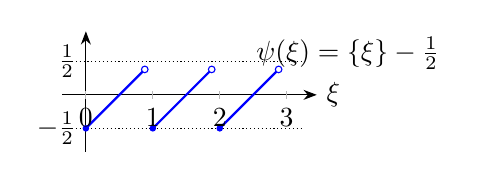
\begin{tikzpicture}[scale=0.85, >=Stealth]
		\draw[->] (-0.35,0) -- (3.45,0) node[right] {$\xi$};
		\draw[->] (0,-0.85) -- (0,0.95);
		\draw[densely dotted] (-0.15,0.5) -- (3.25,0.5);
		\draw[densely dotted] (-0.15,-0.5) -- (3.25,-0.5);
		\node[left] at (0,0.5) {$\frac12$};
		\node[left] at (0,-0.5) {$-\frac12$};
		\foreach \k in {0,1,2} {
			\draw[blue, thick] (\k,-0.5) -- ({\k+0.88},0.38);
			\fill[blue] (\k,-0.5) circle (1.4pt);
			\draw[blue, fill=white] ({\k+0.88},0.38) circle (1.4pt);
			\draw[gray!55] (\k,-0.06) -- (\k,0.06) node[below=3pt, black] {$\k$};
		}
		\draw[gray!55] (3,-0.06) -- (3,0.06) node[below=3pt, black] {$3$};
		\node[right] at (2.4,0.62) {$\psi(\xi)=\{\xi\}-\frac12$};
	\end{tikzpicture}
	\]
	观察到
	\[
		\int_{[x]}^x f(\xi)\,d\xi
		+
		\int_{[x]}^x\psi(\xi)f'(\xi)\,d\xi
		=
		\psi(x)f(x)+\frac12 f([x]).
	\]
	类似地，
	\[
		\int_y^{[y]+1} f(\xi)\,d\xi
		+
		\int_y^{[y]+1}\psi(\xi)f'(\xi)\,d\xi
		=
		-\psi(y)f(y)+\frac12 f([y]+1).
	\]
	最终得到
	\[
		\sum_{y<n\leq x}f(n)
		=
		\int_y^x f(\xi)\,d\xi
		+
		\int_y^x \psi(\xi)f'(\xi)\,d\xi
		+
		\psi(y)f(y)-\psi(x)f(x).
	\]
\end{proof}

\begin{corollary}[原文 Corollary 1]
	有
	\[
		\sum_{n\leq x}\frac1n
		=
		\log x+\gamma+O\left(\frac1x\right),
	\]
	其中
	\[
		\gamma
		=
		1-\int_1^\infty\frac{\{\xi\}}{\xi^2}\,d\xi
	\]
	是 Euler 常数（Euler constant）。
\end{corollary}

\begin{proof}
	由 Euler--Maclaurin 公式，
	\[
	\begin{aligned}
		\sum_{n\leq x}\frac1n
		&=
		1+\sum_{1<n\leq x}\frac1n \\
		&=
		1+\int_1^x\frac1\xi\,d\xi
		-\int_1^x\frac{\psi(\xi)}{\xi^2}\,d\xi
		+\psi(1)-\psi(x)\frac1x \\
		&=
		1+\log x-\int_1^\infty\frac{\psi(\xi)}{\xi^2}\,d\xi
		+\int_x^\infty\frac{\psi(\xi)}{\xi^2}\,d\xi
		-\frac12+O\left(\frac1x\right) \\
		&=
		\frac12+\log x
		-\int_1^\infty\frac{\{\xi\}}{\xi^2}\,d\xi
		+\frac12\int_1^\infty\frac{d\xi}{\xi^2}
		+O\left(\frac1x\right) \\
		&=
		\log x+1-\int_1^\infty\frac{\{\xi\}}{\xi^2}\,d\xi
		+O\left(\frac1x\right) \\
		&=
		\log x+\gamma+O\left(\frac1x\right).
	\end{aligned}
	\]
\end{proof}

\begin{remark}
	我们也可以直接从这个推论看出
	\[
		\gamma
		=
		\lim_{x\to\infty}\left(\sum_{n\leq x}\frac1n-\log x\right).
	\]
	Euler--Maclaurin 公式不允许我们直接估计算术函数的部分和，例如 $\tau(n)$ 和 $\varphi(n)$。
\end{remark}

\section{卷积方法}

\weekmarker{第 2 周}

若
\[
	h=f*g,
\]
并且如果我们可以估计 $g$ 的部分和，那么
\[
\begin{aligned}
	\sum_{n\leq x}h(n)
	&=
	\sum_{n\leq x}\sum_{dm=n}f(d)g(m) \\
	&=
	\sum_{d\leq x}f(d)\sum_{m\leq x/d}g(m).
\end{aligned}
\]

\begin{theorem}[原文 Theorem 3]
	有
	\[
		\sum_{n\leq x}\varphi(n)
		=
		Cx^2+O(x\log x),
		\qquad
		C=\frac{3}{\pi^2}.
	\]
\end{theorem}

\begin{proof}
	回忆
	\[
		\varphi=\operatorname{id}*\mu,
		\qquad
		\varphi(n)=\sum_{d\mid n}\mu(d)\frac nd.
	\]
	于是
	\[
	\begin{aligned}
		\sum_{n\leq x}\varphi(n)
		&=
		\sum_{d\leq x}\mu(d)\sum_{m\leq x/d}m \\
		&=
		\sum_{d\leq x}\mu(d)
		\left(\frac12\left(\frac xd\right)^2+O\left(\frac xd\right)\right) \\
		&=
		\frac{x^2}{2}\sum_{d\leq x}\frac{\mu(d)}{d^2}
		+
		O\left(x\sum_{d\leq x}\frac1d\right) \\
		&=
		\frac{x^2}{2}
		\left(\sum_{d=1}^\infty\frac{\mu(d)}{d^2}
		-\sum_{d>x}\frac{\mu(d)}{d^2}\right)
		+O(x\log x) \\
		&=
		\frac{x^2}{2}\sum_{d=1}^\infty\frac{\mu(d)}{d^2}
		+O\left(x^2\sum_{d>x}\frac1{d^2}+x\log x\right) \\
		&=
		\frac{x^2}{2\zeta(2)}+O(x\log x).
	\end{aligned}
	\]
	由于 $\zeta(2)=\pi^2/6$，所以 $C=3/\pi^2$。
\end{proof}

\begin{remark}
	为了看出
	\[
		\sum_{d=1}^\infty\frac{\mu(d)}{d^2}
		=
		\frac1{\zeta(2)},
	\]
	回忆
	\[
		\zeta(s):=\sum_{n=1}^\infty\frac1{n^s},
		\qquad
		\Re(s)>1.
	\]
	并且
	\[
		\mu=u^{-1},
		\qquad \text{即}\qquad
		\mu*u=I.
	\]
	于是
	\[
		\sum_{n=1}^\infty\frac{(\mu*u)(n)}{n^s}
		=
		\sum_{n=1}^\infty\frac{I(n)}{n^s}
		=
		1.
	\]
	另一方面，由绝对收敛，
	\[
		\sum_{n=1}^\infty\frac{(\mu*u)(n)}{n^s}
		=
		\left(\sum_{d=1}^\infty\frac{\mu(d)}{d^s}\right)
		\left(\sum_{m=1}^\infty\frac1{m^s}\right).
	\]
	因此
	\[
		\sum_{d=1}^\infty\frac{\mu(d)}{d^s}
		=
		\frac1{\zeta(s)}.
	\]
\end{remark}

\begin{theorem}[原文 Theorem，basic case]
	有
	\[
		\sum_{n\leq x}\tau(n)
		=
		x\log x+O(x).
	\]
\end{theorem}

\begin{proof}
	回忆
	\[
		\tau=u*u.
	\]
	于是
	\[
	\begin{aligned}
		\sum_{n\leq x}\tau(n)
		&=
		\sum_{dm\leq x}1 \\
		&=
		\sum_{d\leq x}\left[\frac xd\right] \\
		&=
		\sum_{d\leq x}\left(\frac xd-\left\{\frac xd\right\}\right) \\
		&=
		x\sum_{d\leq x}\frac1d+O\left(\sum_{d\leq x}1\right) \\
		&=
		x\left(\log x+\gamma+O\left(\frac1x\right)\right)+O(x) \\
		&=
		x\log x+O(x).
	\end{aligned}
	\]
\end{proof}

\begin{remark}
	这个定理说 $\tau(n)$ 的平均阶（average order）是 $\log n$，虽然对于单个的 $n$，$\tau(n)$ 可以很大。
\end{remark}

\begin{proposition}[原文 Proposition 1]
	对任意正整数 $A$，存在无穷多个 $n\in\N$，使得
	\[
		(\log n)^A<\tau(n).
	\]
\end{proposition}

\begin{proof}
	取固定互异的素数 $p_1,p_2,\ldots,p_{A+1}$，并考虑
	\[
		n=(p_1p_2\cdots p_{A+1})^r,
	\]
	其中 $r\geq 1$ 是任意整数。则
	\[
		\tau(n)
		=
		\tau(p_1^r)\cdots \tau(p_{A+1}^r)
		=
		(r+1)^{A+1}.
	\]
	另一方面，
	\[
		(\log n)^A
		=
		r^A(\log p_1+\cdots+\log p_{A+1})^A.
	\]
	由于 $r$ 可以任意大，所以存在无穷多个这样的 $n$ 使
	\[
		(\log n)^A\leq \tau(n).
	\]
\end{proof}

\begin{proposition}[原文 Proposition 2]
	对任意给定的 $\varepsilon>0$，存在 $C_\varepsilon>0$，使得对所有 $n\in\N$，
	\[
		\tau(n)\leq C_\varepsilon n^\varepsilon.
	\]
	换句话说，
	\[
		\tau(n)\ll n^\varepsilon
		\qquad\text{或}\qquad
		\tau(n)=O(n^\varepsilon).
	\]
\end{proposition}

\begin{proof}
	原文写作：exercise。
\end{proof}

误差项 $O(x)$ 对
\[
	\sum_{n\leq x}\tau(n)
\]
而言并不令人满意。为了改进它，我们引入 Dirichlet 双曲线方法（Dirichlet hyperbola method）。

\section{Dirichlet 双曲线方法}

\weekmarker{第 2 周}

\begin{theorem}
	设
	\[
		h=f*g.
	\]
	那么对任意 $y\leq x$，有
	\[
	\begin{aligned}
		\sum_{n\leq x}h(n)
		={}&
		\sum_{d\leq y}f(d)\sum_{m\leq x/d}g(m)
		+
		\sum_{m\leq x/y}g(m)\sum_{d\leq x/m}f(d) \\
		&-
		\left(\sum_{d\leq y}f(d)\right)
		\left(\sum_{m\leq x/y}g(m)\right).
	\end{aligned}
	\]
\end{theorem}

\begin{proof}
	我们要计算
	\[
		\sum_{n\leq x}h(n)
		=
		\sum_{dm\leq x}f(d)g(m).
	\]
	手稿图示为双曲线 $dm=x$ 下方的格点区域；先取 $d\leq y$ 的竖条，再取 $m\leq x/y$ 的横条，最后减去被重复计算的矩形。
	\[
	\begin{tikzpicture}[scale=0.85, >=Stealth]
		\draw[->] (0,0) -- (5.7,0) node[right] {$d$};
		\draw[->] (0,0) -- (0,4.7) node[above] {$m$};
		\fill[blue!10] (0.35,0.25) rectangle (1.9,4.25);
		\fill[green!12] (0.35,0.25) rectangle (5.25,2.15);
		\fill[red!16] (0.35,0.25) rectangle (1.9,2.15);
		\draw[thick, domain=0.85:5.25, smooth, variable=\t]
			plot ({\t},{3.95/\t}) node[right] {$dm=x$};
		\draw[dashed] (1.9,0) -- (1.9,4.35) node[above] {$d=y$};
		\draw[dashed] (0,2.15) -- (5.35,2.15) node[right] {$m=x/y$};
		\node at (1.1,3.45) {$d\leq y$};
		\node at (4.0,1.15) {$m\leq x/y$};
		\node at (1.1,1.15) {\scriptsize 重复};
		\fill (1.9,2.15) circle (1.5pt);
	\end{tikzpicture}
	\]
	于是
	\[
	\begin{aligned}
		\sum_{n\leq x}h(n)
		={}&
		\sum_{d\leq y}f(d)\sum_{m\leq x/d}g(m)
		+
		\sum_{m\leq x/y}g(m)\sum_{d\leq x/m}f(d) \\
		&-
		\sum_{d\leq y}f(d)\sum_{m\leq x/y}g(m).
	\end{aligned}
	\]
\end{proof}

\begin{theorem}[原文 Theorem 4]
	有
	\[
		\sum_{n\leq x}\tau(n)
		=
		x\log x+(2\gamma-1)x+O(x^{1/2}).
	\]
\end{theorem}

\begin{proof}
	取 $y=\sqrt{x}$。由于
	\[
		\tau=u*u,
	\]
	由 Dirichlet 双曲线方法得到
	\[
	\begin{aligned}
		\sum_{n\leq x}\tau(n)
		&=
		2\sum_{d\leq \sqrt{x}}\left[\frac xd\right]-[\sqrt{x}]^2 \\
		&=
		2\sum_{d\leq \sqrt{x}}\left(\frac xd+O(1)\right)
		-\bigl(\sqrt{x}+O(1)\bigr)^2 \\
		&=
		2x\sum_{d\leq \sqrt{x}}\frac1d
		+O\left(\sum_{d\leq \sqrt{x}}1\right)
		-x+O(x^{1/2}) \\
		&=
		2x\left(\log\sqrt{x}+\gamma+O(x^{-1/2})\right)
		-x+O(x^{1/2}) \\
		&=
		x\log x+(2\gamma-1)x+O(x^{1/2}).
	\end{aligned}
	\]
\end{proof}

\begin{remark}
	\begin{enumerate}[label=(\alph*)]
		\item 这是 Chen 在 Goldbach 问题（Goldbach problem）证明中的一种“除数交换技巧”（divisor-switching trick）。
		\item 猜想
		\[
			\sum_{n\leq x}\tau(n)
			=
			x\log x+(2\gamma-1)x+O(x^{1/4+\varepsilon}).
		\]
		Voronoi 用 Poisson 求和（Poisson summation）证明了误差项为 $O(x^{1/3}\log x)$。利用指数和（exponential sums）的方法，可以证明误差项为 $O(x^{1/3-\delta})$，其中某个 $\delta>0$。
		\item 在类似方向上，令
		\[
			r_2(n)=\#\{(a,b)\in\mathbb Z^2:a^2+b^2=n\}.
		\]
		那么
		\[
			\sum_{n\leq x}r_2(n)
		\]
		计算以原点为中心、半径为 $\sqrt{x}$ 的圆内格点（lattice point）的个数。
		\[
		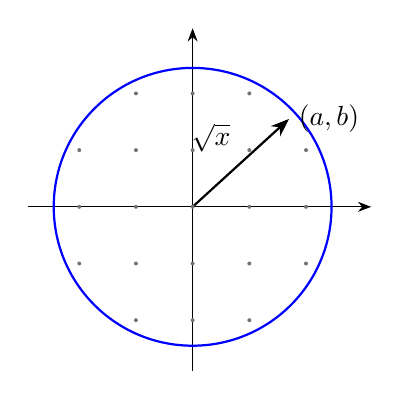
\begin{tikzpicture}[scale=0.72, >=Stealth]
			\draw[->] (-2.9,0) -- (3.15,0);
			\draw[->] (0,-2.9) -- (0,3.15);
			\draw[blue, thick] (0,0) circle (2.45);
			\draw[->, thick] (0,0) -- (1.7,1.55) node[midway, above left] {$\sqrt{x}$};
			\node[right] at (1.7,1.55) {$(a,b)$};
			\foreach \i in {-2,-1,0,1,2} {
				\foreach \j in {-2,-1,0,1,2} {
					\pgfmathsetmacro{\rr}{\i*\i+\j*\j}
					\ifdim \rr pt<6.01pt
						\fill[black!55] (\i,\j) circle (1pt);
					\fi
				}
			}
		\end{tikzpicture}
		\]
		Gauss 证明
		\[
			\sum_{n\leq x}r_2(n)=\pi x+O(x^{1/2}).
		\]
		原文旁注：proof: exercise；conjecture；$O(x^{1/4+\varepsilon})$；Gauss lattice point problem。
	\end{enumerate}
\end{remark}

只有有限的一类算术函数 $h\in A$ 可以写成 Dirichlet 卷积
\[
	h=f*g.
\]
问题是：如果我们知道 $f(n)$ 的部分和
\[
	\sum_{m\leq y}f(m),
\]
那么如何估计乘积
\[
	h(n)=f(n)g(n),
\]
其中 $g$ 是一个比较好的函数？这由 Abel 求和提供。

\section{Abel 求和公式}

\weekmarker{第 2 周}

\begin{theorem}[Abel 求和公式；原文 Theorem 5]
	设 $f$ 是一个算术函数，且 $g:[y,x]\to\CC$ 连续可微。则
	\[
	\begin{aligned}
		\sum_{y<n\leq x}f(n)g(n)
		={}&
		\left(\sum_{n\leq x}f(n)\right)g(x)
		-
		\left(\sum_{n\leq y}f(n)\right)g(y) \\
		&-
		\int_y^x
		\left(\sum_{n\leq \xi}f(n)\right)g'(\xi)\,d\xi.
	\end{aligned}
	\]
\end{theorem}

\begin{proof}
	另一种写法是
	\[
		\sum_{y<n\leq x}f(n)g(n)
		=
		\int_y^x g(\xi)\,d\sum_{y<n\leq \xi}f(n).
	\]
	下面证明手稿中的离散版本。我们可以假设
	\[
		[y]+1\leq [x].
	\]
	记
	\[
		F(x):=\sum_{n\leq x}f(n).
	\]
	则
	\[
	\begin{aligned}
		\text{LHS}
		&=
		\sum_{y<n\leq x}\bigl(F(n)-F(n-1)\bigr)g(n) \\
		&=
		\sum_{y<n\leq x}F(n)g(n)
		-
		\sum_{y+1<n\leq x}F(n-1)g(n) \\
		&=
		\sum_{y<n\leq x-1}F(n)\bigl(g(n)-g(n+1)\bigr)
		+
		F([x])g([x])-F([y])g([y]+1) \\
		&=
		-\sum_{y<n\leq x-1}F(n)\int_n^{n+1}g'(\xi)\,d\xi
		+
		F([x])g([x])-F([y])g([y]+1) \\
		&=
		-\int_{[y]+1}^{[x]}F(\xi)g'(\xi)\,d\xi
		+
		F([x])g([x])-F([y])g([y]+1).
	\end{aligned}
	\]
	最后注意到
	\[
		F(x)g([x])
		=
		F(x)g(x)-\int_{[x]}^xF(\xi)g'(\xi)\,d\xi,
	\]
	以及
	\[
		F(y)g([y]+1)
		=
		F(y)g(y)+\int_y^{[y]+1}F(\xi)g'(\xi)\,d\xi.
	\]
	于是得到
	\[
		\text{LHS}
		=
		-\int_y^x F(\xi)g'(\xi)\,d\xi+F(x)g(x)-F(y)g(y),
	\]
	这正是右边。
\end{proof}

\begin{example}
	回忆在 Theorem 3 中已经证明
	\[
		\sum_{n\leq x}\varphi(n)=Cx^2+O(x\log x),
		\qquad
		C=\frac3{\pi^2}.
	\]
	利用它可以证明下面的结论。
\end{example}

\begin{theorem}[原文 Theorem 6]
	有
	\[
		\sum_{n\leq x}\frac{\varphi(n)}n
		=
		2Cx+O(\log^2 x).
	\]
\end{theorem}

\begin{proof}
	由 Abel 求和，取 $g(\xi)=1/\xi$，得到
	\[
	\begin{aligned}
		\sum_{n\leq x}\varphi(n)\frac1n
		&=
		1+
		\left(\sum_{n\leq x}\varphi(n)\right)\frac1x
		-
		\left(\sum_{n\leq 1}\varphi(n)\right)\cdot 1
		-\int_1^x
		\left(\sum_{n\leq \xi}\varphi(n)\right)
		\left(\frac1\xi\right)'\,d\xi \\
		&=
		\frac1x\bigl(Cx^2+O(x\log x)\bigr)
		+
		\int_1^x
		\bigl(C\xi^2+O(\xi\log \xi)\bigr)\frac1{\xi^2}\,d\xi \\
		&=
		Cx+O(\log x)
		+
		C\int_1^x d\xi
		+
		O\left(\int_1^x\frac{\log \xi}{\xi}\,d\xi\right) \\
		&=
		2Cx+O(\log x)+O(\log^2 x) \\
		&=
		2Cx+O(\log^2 x).
	\end{aligned}
	\]
\end{proof}

至于单个的 $\varphi(n)$，有下面的尖锐下界。

\begin{theorem}[原文 Theorem 7]
	有
	\[
		\varphi(n)\gg \frac{n}{\log\log n}.
	\]
\end{theorem}

\begin{proof}
	回忆
	\[
		\varphi(p^\alpha)=p^\alpha\left(1-\frac1p\right).
	\]
	于是
	\[
		\frac{\varphi(n)}n
		=
		\prod_{p\mid n}\left(1-\frac1p\right).
	\]

	于是
	\begin{equation}
	\begin{aligned}
		\log\frac{\varphi(n)}n
		&=
		\sum_{p\mid n}\log\left(1-\frac1p\right) \\
		&=
		-\sum_{p\mid n}\frac1p
		+
		\sum_{p\mid n}
		\left(\log\left(1-\frac1p\right)+\frac1p\right).
	\end{aligned}
	\tag{*1}
	\end{equation}
	回忆 Taylor 展开
	\[
		\log(1-x)=-x-\frac{x^2}{2}-\cdots.
	\]
	因此
	\[
		\sum_{p\mid n}
		\left(\log\left(1-\frac1p\right)+\frac1p\right)
		\ll
		\sum_{p\mid n}\frac1{p^2}
		\ll
		\sum_{m=1}^\infty\frac1{m^2}
		\ll 1.
	\]
	对于第一项，我们写
	\begin{equation}
		\sum_{p\mid n}\frac1p
		=
		\sum_{\substack{p\mid n\\ p<\log n}}\frac1p
		+
		\sum_{\substack{p\mid n\\ p\geq \log n}}\frac1p.
	\tag{*2}
	\end{equation}
	若记 $p_1,p_2,\ldots,p_{r-\ell}$ 为整除 $n$ 且小于 $\log n$ 的不同素数，并记
	\[
		p_{r-\ell+1},\ldots,p_r
	\]
	为整除 $n$ 且大于 $\log n$ 的素数，其中有 $\ell$ 个，则
	\[
		(\log n)^\ell
		\leq
		\prod_{k=r-\ell+1}^r p_k
		\leq n.
	\]
	从而
	\[
		\ell\leq \frac{\log n}{\log\log n}.
	\]
	把这个用于 $(*2)$ 的第二项，可得
	\[
		\sum_{\substack{p\mid n\\ p>\log n}}\frac1p
		\leq
		\frac1{\log n}\cdot \frac{\log n}{\log\log n}
		=
		O(1).
	\]
	现在考虑第一项。如果我们使用 Mertens 定理（Mertens' theorem）之一：
	\[
		\sum_{p\leq x}\frac1p
		=
		\log\log x+C+O\left(\frac1{\log x}\right),
	\]
	原文旁注：to be proved later，则回到 $(*2)$ 有
	\[
		\sum_{p\mid n}\frac1p
		\leq
		\log\log\log n+O(1).
	\]
	代入 $(*1)$，得到
	\[
		\log\frac{\varphi(n)}n
		\geq
		-\log\log\log n+O(1),
	\]
	因此
	\[
		\frac{\varphi(n)}n\gg \frac1{\log\log n},
	\]
	也就是
	\[
		\varphi(n)\gg \frac{n}{\log\log n}.
	\]
\end{proof}

\begin{remark}
	\begin{enumerate}[label=(\alph*)]
		\item 如果避免使用 Mertens 定理，那么我们会有
		\[
			\sum_{\substack{p\mid n\\ p<\log n}}\frac1p
			\leq
			\sum_{m\leq \log n}\frac1m
			\ll
			\log\log n.
		\]
		这只会推出
		\[
			\frac{\varphi(n)}n\gg \frac1{\log n}.
		\]
		\item 作为练习，可以证明存在一个递增序列 $n_k$，使得
		\[
			\varphi(n_k)\ll \frac{n_k}{\log\log n_k}.
		\]
		因此 Theorem 7 中的下界是 sharp。
	\end{enumerate}
\end{remark}

\chapter{素数分布的初等结果}

\section{素数定理的等价形式}

\weekmarker{第 3 周}

回忆素数定理（Prime Number Theorem）断言：当 $x\to\infty$ 时，
\[
	\pi(x):=\sum_{p\leq x}1\sim \frac{x}{\log x},
\]
或者等价地，
\[
	\lim_{x\to\infty}\frac{\pi(x)}{x/\log x}=1.
\]
Legendre 和 Gauss 曾独立猜想该结论。有时用权重来数素数更有用。为此我们引入两个函数：
\[
	\theta(x)=\sum_{p\leq x}\log p
\]
以及
\[
	\psi(x)=\sum_{n\leq x}\Lambda(n),
\]
其中
\[
	\Lambda(n)=
	\begin{cases}
		\log p, & n=p^k,\ k\geq 1,\\
		0, & \text{otherwise},
	\end{cases}
\]
是 von Mangoldt 函数（von Mangoldt function）。$\psi(x)$ 通常称为 Chebyshev 函数（Chebyshev function）。

回忆
\[
	\log n=\sum_{d\mid n}\Lambda(d),
\]
也即
\[
	\log=\Lambda*u.
\]
由 Möbius 反演（Möbius inversion），这等价于
\[
	\Lambda=\log*\mu.
\]

\begin{lemma}[原文 Lemma 3.1]
	有
	\[
		\psi(x)=\theta(x)+O(x^{1/2}\log x).
	\]
\end{lemma}

\begin{proof}
	由定义，
	\[
	\begin{aligned}
		\psi(x)
		&=
		\sum_{n\leq x}\Lambda(n)
		=
		\sum_{p^m\leq x}\log p \\
		&=
		\sum_{p\leq x}\log p
		+
		\sum_{\substack{p^m\leq x\\ m\geq 2}}\log p \\
		&=
		\theta(x)+
		\sum_{p\leq x^{1/2}}\log p
		\sum_{2\leq m\leq \log x/\log p}1 \\
		&=
		\theta(x)+
		O\left(
			\sum_{p\leq x^{1/2}}\log p\cdot \frac{\log x}{\log p}
		\right) \\
		&=
		\theta(x)+O(x^{1/2}\log x).
	\end{aligned}
	\]
\end{proof}

\begin{theorem}[原文 Theorem 3.2]
	以下三个命题等价：
	\begin{enumerate}[label=(\roman*)]
		\item $\pi(x)\sim \dfrac{x}{\log x}$；
		\item $\theta(x)\sim x$；
		\item $\psi(x)\sim x$。
	\end{enumerate}
\end{theorem}

\begin{proof}
	由 Lemma 3.1，只需要证明 $(i)\Longleftrightarrow(ii)$。

	先证明 $(i)\Rightarrow(ii)$。假设
	\[
		\pi(x)\sim \frac{x}{\log x}.
	\]
	由 Abel 求和，
	\[
	\begin{aligned}
		\theta(x)
		&=
		\sum_{p\leq x}\log p \\
		&=
		\sum_{1<n\leq x}\mathbf 1_{n\in\mathbb P}\log n \\
		&=
		\left(\sum_{p\leq x}1\right)\log x
		-
		\int_1^x
		\frac{\sum_{p\leq y}1}{y}\,dy \\
		&=
		\pi(x)\log x-\int_1^x\frac{\pi(y)}y\,dy \\
		&=
		x+o(x)+
		O\left(\int_1^x\frac{dy}{\log y}\right).
	\end{aligned}
	\]
	由于
	\[
		\int_1^x\frac{dy}{\log y}
		=
		\int_1^{\sqrt{x}}\frac{dy}{\log y}
		+
		\int_{\sqrt{x}}^x\frac{dy}{\log y}
		\ll
		\sqrt{x}+\frac{x}{\log x}
		\ll
		\frac{x}{\log x},
	\]
	所以
	\[
		\theta(x)=x+o(x).
	\]

	反过来，假设
	\[
		\theta(x)\sim x.
	\]
	再次由 Abel 求和，
	\[
	\begin{aligned}
		\pi(x)
		&=
		\sum_{3/2<n\leq x}\log n\,\mathbf 1_{n\in\mathbb P}\cdot \frac1{\log n} \\
		&=
		\left(\sum_{p\leq x}\log p\right)\frac1{\log x}
		+
		\int_{3/2}^{x}
		\frac{\sum_{p\leq y}\log p}{y\log^2 y}\,dy \\
		&=
		\frac{x+o(x)}{\log x}
		+
		\int_{3/2}^{x}\frac{y+o(y)}{y\log^2 y}\,dy \\
		&=
		\frac{x}{\log x}+o\left(\frac{x}{\log x}\right)
		+
		O\left(\int_{3/2}^{x}\frac{dy}{\log^2 y}\right).
	\end{aligned}
	\]
	利用类似的估计，
	\[
		\int_{3/2}^{x}\frac{dy}{\log^2 y}
		\ll
		\frac{x}{\log^2 x}
		=
		o\left(\frac{x}{\log x}\right).
	\]
	因此
	\[
		\pi(x)\sim \frac{x}{\log x}.
	\]
\end{proof}

Chebyshev 对素数定理作出了第一个重要贡献。

\section{Chebyshev 定理}

\begin{theorem}[原文 Theorem 3.3]
	有
	\[
		\pi(x)\asymp \frac{x}{\log x},
		\qquad
		\theta(x)\asymp x,
		\qquad
		\psi(x)\asymp x.
	\]
\end{theorem}

\begin{proof}
	我们先建立
	\[
		\psi(x)\ll x.
	\]
	记
	\[
		S(x):=\sum_{n\leq x}\log n-2\sum_{n\leq x/2}\log n.
	\]
	回忆
	\[
		\sum_{n\leq y}\log n=y\log y-y+O(\log y).
	\]
	因此
	\begin{equation}
	\begin{aligned}
		S(x)
		&=
		x\log x-x
		-2\left(\frac x2\log\frac x2-\frac x2\right)
		+O(\log x) \\
		&=
		(\log 2)x+O(\log x).
	\end{aligned}
	\tag{*1}
	\end{equation}
	又回忆
	\[
		\log=\Lambda*u.
	\]
	那么
	\[
		\sum_{n\leq y}\log n
		=
		\sum_{d\leq y}\Lambda(d)\left[\frac yd\right].
	\]
	于是
	\begin{equation}
	\begin{aligned}
		S(x)
		&=
		\sum_{d\leq x}\Lambda(d)\left[\frac xd\right]
		-
		2\sum_{d\leq x/2}\Lambda(d)\left[\frac{x}{2d}\right] \\
		&=
		\sum_{d\leq x}\Lambda(d)
		\left(\left[\frac xd\right]-2\left[\frac{x}{2d}\right]\right).
	\end{aligned}
	\tag{*2}
	\end{equation}
	注意到对所有 $\alpha\geq 1$，
	\[
		[\alpha]-2\left[\frac\alpha2\right]\in\{0,1\},
	\]
	并且当 $1\leq \alpha<2$ 时，
	\[
		[\alpha]-2\left[\frac\alpha2\right]=1.
	\]
	由 $(*2)$ 得
	\[
		\psi(x)-\psi\left(\frac x2\right)
		=
		\sum_{x/2<d\leq x}\Lambda(d)
		\leq
		S(x)
		\leq
		\sum_{d\leq x}\Lambda(d)=\psi(x).
	\]
	从 $(*1)$ 可见
	\[
		S(x)\sim (\log 2)x,
	\]
	所以
	\[
		\psi(x)\geq S(x)\gg x.
	\]
	另一方面，对每个 $x/2^j$，有
	\[
		\psi\left(\frac{x}{2^j}\right)
		-
		\psi\left(\frac{x}{2^{j+1}}\right)
		\leq
		S\left(\frac{x}{2^j}\right)
		\ll
		\frac{x}{2^j}.
	\]
	对所有 $j\geq 0$ 求和，得到
	\[
		\psi(x)
		=
		\sum_{j=0}^\infty
		\left(
			\psi\left(\frac{x}{2^j}\right)
			-
			\psi\left(\frac{x}{2^{j+1}}\right)
		\right)
		\ll
		x\sum_{j=0}^\infty\frac1{2^j}
		\ll x.
	\]
	因此
	\[
		\psi(x)\asymp x,
	\]
	并且由 Lemma 3.1 也有
	\[
		\theta(x)\asymp x.
	\]

	最后证明
	\[
		\pi(x)\asymp \frac{x}{\log x}.
	\]
	注意
	\[
		\pi(x)=\sum_{p\leq x}1
		\geq
		\frac1{\log x}\sum_{p\leq x}\log p
		\gg
		\frac{x}{\log x}.
	\]
	另一方面，
	\[
		\pi(x)
		\leq
		\sum_{p\leq \sqrt{x}}1
		+
		\sum_{\sqrt{x}<p\leq x}\frac{\log p}{\log\sqrt{x}}
		\leq
		\sqrt{x}+\frac1{\log\sqrt{x}}\theta(x)
		\ll
		\frac{x}{\log x}.
	\]
	定理得证。
\end{proof}

\begin{corollary}[原文 Corollary 3.4]
	令 $p_r$ 为第 $r$ 个素数。则
	\[
		p_r\asymp r\log r.
	\]
\end{corollary}

\begin{proof}
	在上面的定理中取 $x=p_r$，则
	\[
		r=\pi(p_r)\asymp \frac{p_r}{\log p_r}.
	\]
	这推出
	\[
		p_r\asymp r\log p_r\gg r\log r.
	\]
	另一方面，当 $p_r$ 足够大时，
	\[
		\log p_r<p_r^{1/2}.
	\]
	于是
	\[
		p_r\ll r\log p_r\ll r p_r^{1/2},
	\]
	从而
	\[
		p_r\ll r^2.
	\]
	因此
	\[
		p_r\asymp r\log p_r\ll r\log r.
	\]
\end{proof}

\section{Mertens 定理}

\begin{lemma}[原文 Lemma 3.5]
	有
	\[
		\sum_{d\leq x}\frac{\Lambda(d)}d
		=
		\log x+O(1).
	\]
\end{lemma}

\begin{proof}
	从
	\[
		\log=\Lambda*u
	\]
	出发，有
	\[
	\begin{aligned}
		\sum_{n\leq x}\log n
		&=
		\sum_{n\leq x}\sum_{d\mid n}\Lambda(d)
		=
		\sum_{d\leq x}\Lambda(d)\left[\frac xd\right] \\
		&=
		x\sum_{d\leq x}\frac{\Lambda(d)}d+O(x),
	\end{aligned}
	\]
	其中用到了 $\psi(x)\ll x$。另一方面，
	\[
		\sum_{n\leq x}\log n=x\log x-x+O(\log x).
	\]
	两边除以 $x$，得到
	\[
		\sum_{d\leq x}\frac{\Lambda(d)}d=\log x+O(1).
	\]
\end{proof}

\begin{theorem}[原文 Theorem 3.6]
	有
	\[
		\sum_{p\leq x}\frac{\log p}{p}
		=
		\log x+O(1).
	\]
\end{theorem}

\begin{proof}
	比较二者的差：
	\[
	\begin{aligned}
		\left|
			\sum_{d\leq x}\frac{\Lambda(d)}d
			-
			\sum_{p\leq x}\frac{\log p}{p}
		\right|
		&\leq
		\sum_{\substack{p^k\leq x\\ k\geq 2}}\frac{\log p}{p^k} \\
		&\leq
		\sum_{p\leq \sqrt{x}}\log p
		\sum_{k=2}^{\log x/\log p}\frac1{p^k} \\
		&\leq
		\sum_{p\leq \sqrt{x}}
		\log p\cdot
		\frac{1/p^2}{1-1/p} \\
		&\leq
		\sum_p\frac{\log p}{p(p-1)}
		\ll 1.
	\end{aligned}
	\]
	于是由 Lemma 3.5 得到结论。
\end{proof}

\begin{theorem}[原文 Theorem 3.7]
	存在常数 $C$，使得
	\[
		\sum_{p\leq x}\frac1p
		=
		\log\log x+C+O\left(\frac1{\log x}\right).
	\]
\end{theorem}

\begin{proof}
	记
	\[
		E(x):=\sum_{p\leq x}\frac{\log p}{p}-\log x.
	\]
	由 Theorem 3.6 可知
	\[
		E(x)\ll 1.
	\]
	使用 Abel 求和，
	\[
		\begin{aligned}
			\sum_{p\leq x}\frac1p
			&=
			\sum_{3/2<n\leq x}
			\delta_{\mathbb P}(n)\frac{\log n}{n}\cdot\frac1{\log n} \\
			&=
			\left(\sum_{n\leq x}\delta_{\mathbb P}(n)\frac{\log n}{n}\right)\frac1{\log x}
			+
			\int_{3/2}^x
			\frac{\sum_{n\leq y}\delta_{\mathbb P}(n)\frac{\log n}{n}}{y\log^2 y}\,dy \\
		&=
		\frac{\log x+O(1)}{\log x}
		+
		\int_{3/2}^x\frac{\log y+E(y)}{y\log^2 y}\,dy \\
		&=
		\int_{3/2}^x\frac{dy}{y\log y}
		+
		\int_{3/2}^x\frac{E(y)}{y\log^2 y}\,dy
		+
		1+O\left(\frac1{\log x}\right) \\
		&=
		\log\log x-\log\log\frac32
		+
		\int_{3/2}^{\infty}\frac{E(y)}{y\log^2 y}\,dy
		-
		\int_x^\infty\frac{E(y)}{y\log^2 y}\,dy
		+
		1+O\left(\frac1{\log x}\right).
	\end{aligned}
	\]
	其中
	\[
		\int_x^\infty\frac{E(y)}{y\log^2 y}\,dy
		\ll
		\int_x^\infty\frac{dy}{y\log^2 y}
		\ll
		\frac1{\log x},
	\]
	并且
	\[
		\int_{3/2}^{\infty}\frac{E(y)}{y\log^2 y}\,dy
	\]
	是某个常数。于是
	\[
		\sum_{p\leq x}\frac1p
		=
		\log\log x+C+O\left(\frac1{\log x}\right).
	\]
\end{proof}

\begin{theorem}[原文 Theorem 3.8]
	存在某个常数 $A$，使得
	\[
		\prod_{p\leq x}\left(1-\frac1p\right)
		=
		\frac{A}{\log x}
		\left(1+O\left(\frac1{\log x}\right)\right).
	\]
\end{theorem}

\begin{proof}
	我们先考虑
	\[
		\sum_{p\leq x}\log\left(1-\frac1p\right).
	\]
	使用 Taylor 展开，
	\[
	\begin{aligned}
		\sum_{p\leq x}\log\left(1-\frac1p\right)
		&=
		-\sum_{p\leq x}\frac1p
		+
		\sum_{p\leq x}
		\left(\log\left(1-\frac1p\right)+\frac1p\right) \\
		&=
		-\log\log x-C+O\left(\frac1{\log x}\right)
		+
		\sum_p
		\left(\log\left(1-\frac1p\right)+\frac1p\right) \\
		&\qquad
		-
		\sum_{p>x}
		\left(\log\left(1-\frac1p\right)+\frac1p\right).
	\end{aligned}
	\]
	其中
	\[
		\sum_p
		\left(\log\left(1-\frac1p\right)+\frac1p\right)=B
	\]
	是某个常数，因为
	\[
		\sum_p
		\left(\log\left(1-\frac1p\right)+\frac1p\right)
		=
		-\sum_p\sum_{\ell\geq 2}\frac1{\ell p^\ell}
		\ll
		\sum_p\frac1{p^2}
		\ll
		\sum_{n\geq 1}\frac1{n^2}
		\ll 1.
	\]
	并且
	\[
		\sum_{p>x}
		\left(\log\left(1-\frac1p\right)+\frac1p\right)
		\ll
		\sum_{p>x}\frac1{p^2}
		\ll
		\sum_{n>x}\frac1{n^2}
		\ll
		\frac1x.
	\]
	因此
	\[
		\sum_{p\leq x}\log\left(1-\frac1p\right)
		=
		-\log\log x+A'
		+
		O\left(\frac1{\log x}\right).
	\]
	注意由 Taylor 展开，
	\[
		\exp\left(O\left(\frac1{\log x}\right)\right)
		=
		1+O\left(\frac1{\log x}\right).
	\]
	所以
	\[
	\begin{aligned}
		\prod_{p\leq x}\left(1-\frac1p\right)
		&=
		\exp\left(\sum_{p\leq x}\log\left(1-\frac1p\right)\right) \\
		&=
		\exp\left(
			-\log\log x+A'
			+
			O\left(\frac1{\log x}\right)
		\right) \\
		&=
		\frac{A}{\log x}
		\left(1+O\left(\frac1{\log x}\right)\right).
	\end{aligned}
	\]
\end{proof}

接下来会介绍 Mertens 定理的一些应用。

\weekmarker{第 3 周}

\section{\texorpdfstring{\(\omega(n)\) 与 \(\Omega(n)\) 的平均值}{omega(n) 与 Omega(n) 的平均值}}

回忆，$\omega(n)$ 表示 $n$ 的不同素因子的个数，而 $\Omega(n)$ 表示 $n$ 的素因子的总个数，也就是说按重数计算。

对于单个的 $n$，$\omega(n)$ 与 $\Omega(n)$ 的行为可能相当不规则。但是在平均意义下，我们有下面的结果。

\begin{theorem}[原文 Theorem 3.9]
	有
	\[
		\sum_{n\leq x}\omega(n)
		=
		x\log\log x+Cx+O\left(\frac{x}{\log x}\right),
	\]
	并且
	\[
		\sum_{n\leq x}\Omega(n)
		=
		x\log\log x+C'x+O\left(\frac{x}{\log x}\right).
	\]
\end{theorem}

\begin{proof}
	先考虑 $\omega(n)$。有
	\[
	\begin{aligned}
		\sum_{n\leq x}\omega(n)
		&=
		\sum_{n\leq x}\sum_{p\mid n}1
		=
		\sum_{p\leq x}\sum_{\substack{n\leq x\\ p\mid n}}1 \\
		&=
		\sum_{p\leq x}\left[\frac xp\right]
		=
		x\sum_{p\leq x}\frac1p+O\left(\sum_{p\leq x}1\right) \\
		&=
		x\left(\log\log x+C+O\left(\frac1{\log x}\right)\right)
		+O\left(\frac{x}{\log x}\right) \\
		&=
		x\log\log x+Cx+O\left(\frac{x}{\log x}\right),
	\end{aligned}
	\]
	其中使用了 Mertens 定理以及 Chebyshev 定理给出的 $\pi(x)\ll x/\log x$。

	再考虑 $\Omega(n)$。有
	\[
	\begin{aligned}
		\sum_{n\leq x}\Omega(n)
		&=
		\sum_{n\leq x}\sum_{p^k\mid n}1
		=
		\sum_{p^k\leq x}\sum_{\substack{n\leq x\\ p^k\mid n}}1 \\
		&=
		\sum_{p^k\leq x}\left[\frac{x}{p^k}\right] \\
		&=
		\sum_{p\leq x}\left[\frac xp\right]
		+
		\sum_{\substack{p^k\leq x\\ k\geq 2}}
		\left[\frac{x}{p^k}\right] \\
		&=
		x\log\log x+Cx+O\left(\frac{x}{\log x}\right)
		+
		x\sum_{\substack{p^k\leq x\\ k\geq 2}}\frac1{p^k}
		+
		O\left(\sum_{\substack{p^k\leq x\\ k\geq 2}}1\right).
	\end{aligned}
	\]
	原文在边栏证明下面这个估计：
	\[
		\sum_{\substack{p^k>x\\ k\geq 2}}\frac1{p^k}
		=
		O\left(x^{-1/2}\right).
	\]
	证明如下。若 $p\leq x^{1/2}$，则 $\log x/\log p\geq 2$，所以
	\[
		\sum_{\substack{k\geq 2\\ p^k>x}}\frac1{p^k}
		\leq
		\frac{1}{p^{\log x/\log p}}\cdot\frac1{1-1/p}
		\ll
		\frac1x\cdot\frac1{1-1/p}.
	\]
	若 $p>x^{1/2}$，则从 $k=2$ 起估计即可。因此
	\[
	\begin{aligned}
		\sum_{\substack{p^k>x\\ k\geq 2}}\frac1{p^k}
		&\ll
		\frac1x\sum_{p\leq x^{1/2}}\frac1{1-1/p}
		+
		\sum_{p>x^{1/2}}\frac1{p^2}\frac1{1-1/p} \\
		&\ll
		\frac1x\sum_{p\leq x^{1/2}}1
		+
		\sum_{n>x^{1/2}}\frac1{n^2}
		\ll
		x^{-1/2}.
	\end{aligned}
	\]
	于是
	\[
		\sum_{\substack{p^k\leq x\\ k\geq 2}}\frac1{p^k}
		=
		\sum_{\substack{p,k\\ k\geq 2}}\frac1{p^k}
		+
		O\left(x^{-1/2}\right)
		=
		C_1+O\left(x^{-1/2}\right).
	\]
	此外
	\[
		\sum_{\substack{p^k\leq x\\ k\geq 2}}1
		\ll
		\sum_{p\leq x^{1/2}}\frac{\log x}{\log p}
		\ll
		x^{1/2}\log x.
	\]
	因此
	\[
	\begin{aligned}
		\sum_{n\leq x}\Omega(n)
		&=
		x\log\log x+Cx+O\left(\frac{x}{\log x}\right)
		+
		C_1x+O\left(x^{1/2}\right)
		+
		O\left(x^{1/2}\log x\right) \\
		&=
		x\log\log x+C'x+O\left(\frac{x}{\log x}\right).
	\end{aligned}
	\]
\end{proof}

\begin{theorem}[原文 Theorem 3.10]
	有
	\[
		\sum_{n\leq x}\omega^2(n)
		=
		x(\log\log x)^2+O(x\log\log x).
	\]
\end{theorem}

\begin{proof}
	考虑 $n$ 的不同素因子组成的有序对 $(p,q)$ 的个数，其中约定 $(p,q)$ 与 $(q,p)$ 作为两个不同的有序对来计算。于是有 $\omega(n)$ 种选择 $p$，当 $p$ 固定后有 $\omega(n)-1$ 种选择 $q$。因此
	\[
		\omega(n)(\omega(n)-1)
		=
		\sum_{\substack{p\mid n,\ q\mid n\\ p\neq q}}1.
	\]
	对 $n\leq x$ 求和，得到
	\[
	\begin{aligned}
		\sum_{n\leq x}\omega(n)(\omega(n)-1)
		&=
		\sum_{n\leq x}
		\sum_{\substack{p\mid n,\ q\mid n\\ p\neq q}}1 \\
		&=
		\sum_{\substack{pq\leq x\\ p\neq q}}
		\sum_{\substack{n\leq x\\ pq\mid n}}1
		=
		\sum_{\substack{pq\leq x\\ p\neq q}}
		\left[\frac{x}{pq}\right] \\
		&=
		x\sum_{\substack{pq\leq x\\ p\neq q}}\frac1{pq}
		+
		O\left(
			\sum_{p\leq x}\sum_{q\leq x/p}1
		\right).
	\end{aligned}
	\]
	其中
	\[
		\sum_{p\leq x}\sum_{q\leq x/p}1
		\ll
		x\sum_{p\leq x}\frac1p
		\ll
		x\log\log x,
	\]
	这里再次使用 Mertens 定理。

	注意
	\[
		\left(\sum_{p\leq x^{1/2}}\frac1p\right)^2
		-
		\sum_{p\leq x^{1/2}}\frac1{p^2}
		\leq
		\sum_{\substack{pq\leq x\\ p\neq q}}\frac1{pq}
		\leq
		\left(\sum_{p\leq x}\frac1p\right)^2.
	\]
	并且
	\[
		\left(\sum_{p\leq x}\frac1p\right)^2
		=
		(\log\log x+O(1))^2
		=
		(\log\log x)^2+O(\log\log x),
	\]
	以及
	\[
		\left(\sum_{p\leq x^{1/2}}\frac1p\right)^2
		=
		(\log\log x^{1/2}+O(1))^2
		=
		(\log\log x)^2+O(\log\log x).
	\]
	因此
	\[
		\sum_{\substack{pq\leq x\\ p\neq q}}\frac1{pq}
		=
		(\log\log x)^2+O(\log\log x).
	\]
	于是
	\[
		\sum_{n\leq x}\omega(n)(\omega(n)-1)
		=
		x(\log\log x)^2+O(x\log\log x).
	\]
	最后，
	\[
	\begin{aligned}
		\sum_{n\leq x}\omega^2(n)
		&=
		\sum_{n\leq x}\omega(n)(\omega(n)-1)
		+
		\sum_{n\leq x}\omega(n) \\
		&=
		x(\log\log x)^2+O(x\log\log x).
	\end{aligned}
	\]
\end{proof}

由 Theorem 3.9 和 Theorem 3.10，我们有充分理由相信，对大多数 $n$，$\omega(n)$ 的行为像
\[
	\omega(n)\sim \log\log n.
\]
这一点可以进一步说明如下。

\weekmarker{第 4 周}

\begin{theorem}[原文 Theorem 3.11]
	给定任意 $\varepsilon>0$。满足
	\[
		\left|\omega(n)-\log\log n\right|
		>
		(\log\log n)^{1/2+\varepsilon}
	\]
	的 $n\in[1,x]$ 的个数至多是 $o(x)$。
\end{theorem}

\begin{proof}
	我们回忆 Chebyshev 不等式（Chebyshev inequality）的一个版本。设 $(X,\Sigma,\mu)$ 是一个测度空间（measure space），且 $f$ 可测。对 $0<p<\infty$，有
	\[
		\mu\left(\left\{x\in X:|f(x)|>t\right\}\right)
		\leq
		\frac1{t^p}\int_{\{|f|>t\}}|f|^p\,d\mu.
	\]
	取 $p=2$，则
	\[
	\begin{aligned}
		&\#\left\{n\in[1,x]:
		\left|\omega(n)-\log\log x\right|
		>
		(\log\log x)^{1/2+\varepsilon}
		\right\} \\
		&\qquad\leq
		\frac1{(\log\log x)^{1+2\varepsilon}}
		\sum_{n\leq x}\left(\omega(n)-\log\log x\right)^2.
	\end{aligned}
	\]
	\begin{remark}
		原文红色旁注写有 “open square \& apply Abel”，指向上面的平方和估计。
	\end{remark}

	将区间分成
	\[
		[1,x]=[1,x^{1/e}]\cup (x^{1/e},x].
	\]
	其中 $[1,x^{1/e}]$ 中的整数个数是 $o(x)$。对于 $n\in(x^{1/e},x]$，有
	\[
		\log\log x-1=\log\log x^{1/e}<\log\log n\leq \log\log x.
	\]
	因此只需证明满足
	\[
		\left|\omega(n)-\log\log x\right|
		>
		(\log\log x)^{1/2+\varepsilon}
	\]
	的 $n\in[1,x]$ 的个数 $M$ 是 $o(x)$。

	展开平方：
	\[
	\begin{aligned}
		\sum_{n\leq x}\left(\omega(n)-\log\log x\right)^2
		&=
		\sum_{n\leq x}\omega^2(n)
		-
		2\log\log x\sum_{n\leq x}\omega(n)\\
		&\qquad+
		[x](\log\log x)^2.
	\end{aligned}
	\]
	由 Theorem 3.9 和 Theorem 3.10，
	\[
	\begin{aligned}
		\sum_{n\leq x}\left(\omega(n)-\log\log x\right)^2
		&=
		x(\log\log x)^2+O(x\log\log x)\\
		&\quad
		-2\log\log x\left(x\log\log x+O(x)\right)\\
		&\quad
		+x(\log\log x)^2+O\left((\log\log x)^2\right)\\
		&=
		O(x\log\log x).
	\end{aligned}
	\]
	因此
	\[
		M
		\ll
		\frac{x\log\log x}{(\log\log x)^{1+2\varepsilon}}
		\ll
		\frac{x}{(\log\log x)^{2\varepsilon}}
		=
		o(x).
	\]
\end{proof}

\begin{remark}
	另一种做法是直接展开上面标记的平方项，并用 Abel 求和来估计
	\[
		\sum_{n\leq x}\log\log n\cdot \omega(n),
	\]
	从而得到同样的结果。
\end{remark}

\begin{remark}
	\begin{enumerate}[label=(\alph*)]
		\item 同样的结论对 $\Omega(n)$ 也成立。
		\item Theorem 3.11 说明，对几乎所有 $n\in[1,x]$，都有
		\[
			\omega(n),\ \Omega(n)\sim \log\log n.
		\]
		\item Erdős--Kac 定理（Erdős--Kac theorem, 1940）说明变量
		\[
			\frac{\omega(n)-\log\log n}{\sqrt{\log\log n}}
		\]
		服从正态分布（normal distribution）。这是概率数论（Probabilistic Number Theory）的一个基本定理。
	\end{enumerate}
\end{remark}

\section{Bertrand 公设}

Bertrand 在 1845 年猜想：对每个 $n\geq 2$，总存在一个素数 $p$，使得
\[
	n<p\leq 2n.
\]
这个猜想由 Chebyshev 在 1852 年证明。

\begin{theorem}[Bertrand 公设；原文 Theorem 3.12]
	对任意 $n\geq 2$，至少存在一个素数
	\[
		p\in(n,2n].
	\]
\end{theorem}

\begin{remark}
	可以从 Mertens 定理推出一个弱一些的版本。由
	\[
		\sum_{p\leq x}\frac{\log p}{p}=\log x+O(1)
	\]
	可知，存在某个 $A>0$，使得
	\[
		\log n-A
		<
		\sum_{p\leq n}\frac{\log p}{p}
		\leq
		\log n+A.
	\]
	于是
	\[
	\begin{aligned}
		\sum_{n<p\leq e^{2A}n}\frac{\log p}{p}
		&=
		\sum_{p\leq e^{2A}n}\frac{\log p}{p}
		-
		\sum_{p\leq n}\frac{\log p}{p}\\
		&>
		\log(e^{2A}n)-A-\log n-A
		=
		0.
	\end{aligned}
	\]
	因此存在素数 $p\in(n,e^{2A}n]$。
\end{remark}

为了证明 Theorem 3.12，我们先回忆下面的事实。

\begin{lemma}[原文 Lemma 3.13]
	令 $n\in\N$。记
	\[
		n!:=\prod_{p\leq n}p^{h(p,n)}.
	\]
	则
	\[
		h(p,n)=\sum_{r=1}^{\infty}\left[\frac{n}{p^r}\right].
	\]
\end{lemma}

\begin{proof}
	记 $p^r\Vert a$ 表示 $p^r\mid a$ 但是 $p^{r+1}\nmid a$。在 $[1,n]$ 中被 $p^r$ 整除的整数个数为
	\[
		\left[\frac n{p^r}\right].
	\]
	在 $[1,n]$ 中被 $p^r$ 整除但不被 $p^{r+1}$ 整除的整数个数为
	\[
		\left[\frac n{p^r}\right]
		-
		\left[\frac n{p^{r+1}}\right].
	\]
	于是
	\[
		n!=1\cdot 2\cdots n=\prod_{p\leq n}p^{h(p,n)},
	\]
	其中
	\[
	\begin{aligned}
		h(p,n)
		&=
		1\left(\left[\frac np\right]-\left[\frac n{p^2}\right]\right)
		+
		2\left(\left[\frac n{p^2}\right]-\left[\frac n{p^3}\right]\right)\\
		&\quad+
		3\left(\left[\frac n{p^3}\right]-\left[\frac n{p^4}\right]\right)
		+\cdots\\
		&=
		\left[\frac np\right]
		+
		\left[\frac n{p^2}\right]
		+
		\left[\frac n{p^3}\right]
		+\cdots
		=
		\sum_{r=1}^{\infty}\left[\frac{n}{p^r}\right].
	\end{aligned}
	\]
\end{proof}

\begin{lemma}[原文 Lemma 3.14]
	对每个正整数 $n$，有
	\[
		\prod_{p\leq n}p<4^n.
	\]
\end{lemma}

\begin{proof}
	对 $n$ 归纳。$n=1$ 或 $n=2$ 时显然成立。假设结论对 $1,2,\ldots,n-1$ 都成立，其中 $n\geq 3$，我们要证明结论对 $n$ 成立。

	只需考虑 $n$ 为奇数的情形。因为若 $n$ 为偶数，则
	\[
		\prod_{p\leq n}p
		=
		\prod_{p\leq n-1}p
		<
		4^{n-1}<4^n.
	\]
	写 $n=2m+1$。注意二项式系数
	\[
		\binom{2m+1}{m+1}
		=
		\frac{(2m+1)!}{m!(m+1)!}
	\]
	被每一个素数 $p\in[m+2,2m+1]$ 整除，从而被这些素数的乘积整除。因此
	\[
		\prod_{p\leq 2m+1}p
		\leq
		\prod_{p\leq m+1}p\binom{2m+1}{m+1}
		\leq
		4^{m+1}\binom{2m+1}{m+1}.
	\]
	注意 $\binom{2m+1}{m+1}$ 与 $\binom{2m+1}{m}$ 都出现在
	\[
		(1+1)^{2m+1}=2^{2m+1}
	\]
	的展开中，并且二者相等。因此
	\[
		2\binom{2m+1}{m+1}\leq 2^{2m+1},
	\]
	从而
	\[
		\prod_{p\leq 2m+1}p
		\leq
		2^{2m}\cdot 4^{m+1}
		=
		4^m\cdot 4^{m+1}
		=
		4^{2m+1}.
	\]
\end{proof}

\begin{remark}
	若使用 Chebyshev 定理，则可得到
	\[
		\prod_{p\leq n}p
		\leq
		n^{\pi(n)}
		\leq
		n^{1.11\, n/\log n}
		=
		(e^{1.11})^n
		<
		3.04^n,
	\]
	这比上面的估计略好。
\end{remark}

\begin{lemma}[原文 Lemma 3.15]
	若 $n\geq 3$ 且
	\[
		\frac23 n<p\leq n,
	\]
	则 $p\nmid \binom{2n}{n}$。
\end{lemma}

\begin{proof}
	由
	\[
		\binom{2n}{n}=\frac{(2n)!}{(n!)^2}
	\]
	和 Lemma 3.13 可知，如果
	\[
		p^{e(p,n)}\Vert \binom{2n}{n},
	\]
	则
	\[
		e(p,n)=\sum_{r\geq 1}\left(\left[\frac{2n}{p^r}\right]-2\left[\frac n{p^r}\right]\right).
	\]
	因为 $n\geq 3$ 且 $p>2n/3$，所以 $p\geq 3$，并且
	\[
		p^2>p\cdot \frac{2n}{3}>2n.
	\]
	于是对 $r\geq 2$，
	\[
		\left[\frac{2n}{p^r}\right]-2\left[\frac n{p^r}\right]=0.
	\]
	又由 $2n/3<p\leq n$，得到
	\[
		2<\frac{2n}{p}<3,
		\qquad
		1\leq \frac np<\frac32.
	\]
	因此只剩下 $r=1$ 的项：
	\[
		e(p,n)
		=
		\left[\frac{2n}{p}\right]
		-
		2\left[\frac np\right]
		=
		2-2=0.
	\]
	所以这样的 $p$ 在 $\binom{2n}{n}$ 中的指数为 $0$，即不整除 $\binom{2n}{n}$。
\end{proof}

\begin{proof}[Theorem 3.12 的证明]
	若 $n$ 较小，例如 $n\leq 500$，可以手动检验。下面设 $n>500$。反设结论不成立，即不存在素数
	\[
		p\in(n,2n].
	\]
	于是
	\[
		\binom{2n}{n}
		=
		\frac{(2n)!}{(n!)^2}
		=
		\prod_{p\leq 2n}p^{e(p,n)}
		=
		\prod_{p\leq n}p^{e(p,n)}
	\]
	由反设得到，其中
	\[
		e(p,n)=\sum_{r\geq 1}\left(\left[\frac{2n}{p^r}\right]-2\left[\frac n{p^r}\right]\right).
	\]
	对所有 $a$，有
	\[
		[2a]-2[a]\leq 1.
	\]
	若 $p^r\leq 2n$，则
	\[
		r\leq \frac{\log(2n)}{\log p},
	\]
	所以
	\[
		p^{e(p,n)}
		\leq
		p^{\log(2n)/\log p}
		\leq
		2n.
	\]
	特别地，对所有 $p\leq \sqrt{2n}$，有 $p^{e(p,n)}\leq 2n$。

	若 $2n/3<p\leq n$，由 Lemma 3.15 得 $e(p,n)=0$，也就是 $p^{e(p,n)}=1$。若 $\sqrt{2n}\leq p\leq 2n/3$，则 $p^2>2n$，并且
	\[
		e(p,n)
		=
		\sum_{r\geq 1}\left(\left[\frac{2n}{p^r}\right]-2\left[\frac n{p^r}\right]\right)
		=
		\left[\frac{2n}{p}\right]-2\left[\frac np\right]
		\leq 1.
	\]
	因此
	\[
	\begin{aligned}
		\binom{2n}{n}
		&=
		\prod_{p\leq n}p^{e(p,n)}\\
		&\leq
		\prod_{p\leq \sqrt{2n}}p^{e(p,n)}
		\prod_{\sqrt{2n}<p\leq (2/3)n}p\\
		&\leq
		(2n)^{\pi(\sqrt{2n})}
		\prod_{p\leq (2/3)n}p\\
		&\leq
		(2n)^{\sqrt{2n}-1}4^{(2/3)n}.
	\end{aligned}
	\]
	另一方面，$\binom{2n}{n}$ 是
	\[
		(1+1)^{2n}=4^n
	\]
	展开中 $2n+1$ 个项里最大的项。因此原文写道
	\[
		2n\binom{2n}{n}>4^n.
	\]
	于是
	\[
		\frac{4^n}{2n}
		<
		\binom{2n}{n}
		<
		(2n)^{\sqrt{2n}-1}4^{(2/3)n}.
	\]
	从而
	\[
		4^{n/3}<(2n)^{\sqrt{2n}},
	\]
	即
	\[
		\frac n3\log 4<\sqrt{2n}\log(2n).
	\]
	所以
	\[
		\sqrt n<\frac{3\sqrt2}{\log 4}\log(2n).
	\]
	原文说明这个不等式在 $n\geq 427$ 时不成立。由于我们已假设 $n>500$，矛盾。
\end{proof}

\section{\texorpdfstring{\(\mu(n)\) 的部分和}{mu(n) 的部分和}}

回忆，在 Theorem 3.2 中我们已经证明素数定理（Prime Number Theorem, PNT）等价于
\[
	\theta(x)=\sum_{p\leq x}\log p\sim x
\]
以及
\[
	\psi(x)=\sum_{n\leq x}\Lambda(n)\sim x.
\]
现在我们想说明 $\mu(n)$ 的部分和（partial sum）
\[
	M(x):=\sum_{n\leq x}\mu(n)
\]
也与 PNT 密切相关。

\begin{lemma}[原文 Lemma 3.16]
	对任意 $x\geq 1$，有
	\[
		\left|\sum_{n\leq x}\frac{\mu(n)}n\right|\leq 1.
	\]
\end{lemma}

\begin{proof}
	我们可以假设 $x\in\N$。回忆 $\mu=u^{-1}$，也就是说
	\[
		(\mu*u)(n)=\sum_{d\mid n}\mu(d)=I(n)
		=
		\begin{cases}
			1, & n=1,\\
			0, & \text{else}.
		\end{cases}
	\]
	于是
	\[
	\begin{aligned}
		1
		&=
		\sum_{n\leq x}I(n)
		=
		\sum_{n\leq x}\sum_{d\mid n}\mu(d)
		=
		\sum_{d\leq x}\mu(d)\sum_{\substack{n\leq x\\ d\mid n}}1\\
		&=
		\sum_{d\leq x}\mu(d)\left[\frac xd\right]
		=
		x\sum_{d\leq x}\frac{\mu(d)}d
		-
		\sum_{d\leq x}\mu(d)\left\{\frac xd\right\}.
	\end{aligned}
	\]
	因此
	\[
		x\left|\sum_{d\leq x}\frac{\mu(d)}d\right|
		\leq
		1+\sum_{d\leq x-1}\left|\mu(d)\left\{\frac xd\right\}\right|
		\leq
		x,
	\]
	其中用到 $\{x/x\}=0$。从而得到结论。
\end{proof}

定义
\[
	H(x):=\sum_{n\leq x}\mu(n)\log n.
\]

\begin{lemma}[原文 Lemma 3.17]
	有
	\[
		\frac{M(x)}x
		=
		\frac{H(x)}{x\log x}+o(1).
	\]
\end{lemma}

\begin{proof}
	由 Abel 求和，
	\[
		H(x)
		=
		\sum_{1<n\leq x}\mu(n)\log n
		=
		M(x)\log x-\int_1^x\frac{M(y)}y\,dy.
	\]
	因此
	\[
		\frac{M(x)}x
		=
		\frac{H(x)}{x\log x}
		+
		\frac1{x\log x}\int_1^x\frac{M(y)}y\,dy
		=
		\frac{H(x)}{x\log x}
		+
		O\left(\frac1{\log x}\right),
	\]
	因为 $|M(y)|\leq y$。
\end{proof}

\begin{theorem}[原文 Theorem 3.18]
	素数定理蕴含
	\[
		\lim_{x\to\infty}\frac{M(x)}x=0.
	\]
	也就是说，
	\[
		\sum_{n\leq x}\mu(n)=o(x).
	\]
\end{theorem}

\begin{proof}
	我们以如下形式使用 PNT：
	\begin{equation}
		\psi(x)=\sum_{n\leq x}\Lambda(n)\sim x. \tag{*1}
	\end{equation}
	由 Lemma 3.17，要证明 $\sum_{n\leq x}\mu(n)=o(x)$，只需证明
	\[
		\lim_{x\to\infty}\frac{H(x)}{x\log x}=0,
	\]
	其中
	\[
		H(x)=\sum_{n\leq x}\mu(n)\log n.
	\]
	为此回忆
	\[
		\Lambda(n)
		=
		\sum_{d\mid n}\mu(d)\log\frac nd
		=
		\log n\sum_{d\mid n}\mu(d)
		-
		\sum_{d\mid n}\mu(d)\log d.
	\]
	由 Möbius 反演（Möbius inversion），
	\[
		\mu(n)\log n=-(\mu*\Lambda)(n).
	\]
	所以
	\[
	\begin{aligned}
		H(x)
		&=
		\sum_{n\leq x}\mu(n)\log n
		=
		-\sum_{n\leq x}(\mu*\Lambda)(n)\\
		&=
		-\sum_{n\leq x}\sum_{d\mid n}\mu(d)\Lambda\left(\frac nd\right)
		=
		-\sum_{d\leq x}\mu(d)\sum_{m\leq x/d}\Lambda(m)\\
		&=
		-\sum_{d\leq x}\mu(d)\psi\left(\frac xd\right).
	\end{aligned}
	\]
	式 (*1) 蕴含
	\[
		\psi(x)-x=o(x),
	\]
	也就是说，对任意 $\varepsilon>0$，存在 $x_0$，使得当 $x\geq x_0$ 时，
	\[
		|\psi(x)-x|\leq \varepsilon x.
	\]
	记 $R(y):=\psi(y)-y$。将上式分解为
	\[
	\begin{aligned}
		H(x)
		&=
		-\sum_{d\leq x/x_0}\mu(d)\left(\frac xd+R\left(\frac xd\right)\right)
		-\sum_{x/x_0<d<x}\mu(d)\psi\left(\frac xd\right).
	\end{aligned}
	\]
	于是
	\[
	\begin{aligned}
		|H(x)|
		&\leq
		x\left|\sum_{d\leq x/x_0}\frac{\mu(d)}d\right|
		+
		\sum_{d\leq x/x_0}\left|R\left(\frac xd\right)\right|
		+
		\sum_{x/x_0<d<x}\psi\left(\frac xd\right)\\
		&\leq
		x+\varepsilon x\sum_{d\leq x/x_0}\frac1d
		+
		O\left(x\sum_{x/x_0<d<x}\frac1d\right)\\
		&\leq
		x+\varepsilon x\log x+O(x)+O(x\log x_0).
	\end{aligned}
	\]
	因此
	\[
		\limsup_{x\to\infty}
		\left|\frac{H(x)}{x\log x}\right|
		\leq
		\varepsilon.
	\]
	由于 $\varepsilon$ 任意，得到
	\[
		\lim_{x\to\infty}\frac{H(x)}{x\log x}=0.
	\]
\end{proof}

\begin{theorem}[原文 Theorem 3.19]
	关系
	\begin{equation}
		M(x)=\sum_{n\leq x}\mu(n)=o(x)\qquad (x\to\infty). \tag{*2}
	\end{equation}
	蕴含素数定理。
\end{theorem}

\begin{proof}
	我们要证明 $M(x)=o(x)$ 蕴含
	\[
		\psi(x)=\sum_{n\leq x}\Lambda(n)\sim x.
	\]
	证明依赖恒等式
	\[
		\Lambda=\log *\mu.
	\]
	原文先给出一个 “first unsuccessful attempt”。直接写
	\[
	\begin{aligned}
		\sum_{n\leq x}\Lambda(n)
		&=
		\sum_{n\leq x}\sum_{d\mid n}\log d\,\mu\left(\frac nd\right)
		=
		\sum_{d\leq x}\log d\sum_{m\leq x/d}\mu(m).
	\end{aligned}
	\]
	由 (*2)，对任意 $\varepsilon>0$，仅能推出
	\[
		|\psi(x)|
		\leq
		\varepsilon\sum_{d\leq x}\log d\cdot \frac xd
		\ll
		\varepsilon x\log^2 x,
	\]
	这还不足以推出 $\psi(x)\sim x$。

	思路是：在
	\[
		\Lambda(n):=\sum_{md=n}\log m\,\mu(d)
	\]
	中，用某个“好的函数” $f(n)$ 逼近 $\log n$。我们选择的 $f(n)$ 具有如下形状：
	\[
		f(n):=\tau(n)-2\gamma,
	\]
	其中
	\[
		\tau(n)=(u*u)(n)=\sum_{d\mid n}1
	\]
	是除数函数。选择它的动机是：$f(n)$ 的部分和可以很好地逼近 $\log n$ 的部分和。确实，
	\[
	\begin{aligned}
		\sum_{n\leq x}f(n)
		&=
		\sum_{n\leq x}\tau(n)-2\gamma\sum_{n\leq x}1\\
		&=
		x\log x+(2\gamma-1)x+O(\sqrt{x})
		-2\gamma x+O(1)\\
		&=
		x\log x-x+O(\sqrt{x}),
	\end{aligned}
	\]
	而
	\[
		\sum_{n\leq x}\log n
		=
		x\log x-x+O(\log x).
	\]
	因此，如果定义余项 $r(n)$ 为
	\[
		\log=f+r=u*u-2\gamma+r,
	\]
	则
	\begin{equation}
		\sum_{n\leq x}r(n)=O(\sqrt{x}). \tag{*3}
	\end{equation}

	现在把 $\log$ 替换为 $f+r$，得到
	\[
	\begin{aligned}
		\Lambda
		&=
		\mu*\log
		=
		\mu*(u*u-2\gamma+r)\\
		&=
		(\mu*u)*u-2\gamma(\mu*u)+\mu*r\\
		&=
		I*u-2\gamma I+\mu*r
		=
		u-2\gamma I+\mu*r,
	\end{aligned}
	\]
	其中 $u(n)=1$ 对所有 $n\in\N$，而
	\[
		I(n)=
		\begin{cases}
			1, & n=1,\\
			0, & \text{else}.
		\end{cases}
	\]
	于是
	\[
		\sum_{n\leq x}\Lambda(n)
		=
		\sum_{n\leq x}1-2\gamma+\sum_{n\leq x}(\mu*r)(n)
		=
		x+O(1)+E(x),
	\]
	其中
	\[
		E(x):=\sum_{n\leq x}(\mu*r)(n).
	\]
	要证明 $\sum_{n\leq x}\Lambda(n)\sim x$，只需证明
	\[
		E(x)=o(x).
	\]

	我们使用 Dirichlet 双曲线方法（Dirichlet hyperbola method）。回忆对任意 $\varepsilon y\leq x$，有
	\[
	\begin{aligned}
		\sum_{n\leq x}(f*g)(n)
		&=
		\sum_{d\leq y}f(d)\sum_{m\leq x/d}g(m)
		+
		\sum_{m\leq x/y}g(m)\sum_{d\leq x/m}f(d)\\
		&\qquad
		-
		\left(\sum_{d\leq y}f(d)\right)
		\left(\sum_{m\leq x/y}g(m)\right).
	\end{aligned}
	\]
	将其应用到 $r*\mu$。记
	\[
		R(y):=\sum_{d\leq y}r(d).
	\]
	由 (*3)，存在常数 $C>0$，使得
	\[
		|R(y)|\leq C\sqrt y.
	\]
	于是
	\[
		E(x)=\Sigma_1+\Sigma_2-\Sigma_3,
	\]
	其中
	\[
		\Sigma_1=\sum_{d\leq y}r(d)M\left(\frac xd\right),
	\]
	\[
		\Sigma_2=\sum_{m\leq x/y}\mu(m)R\left(\frac xm\right),
	\]
	并且
	\[
		\Sigma_3=R(y)M\left(\frac xy\right).
	\]
	只需证明：对任意 $\varepsilon>0$，存在 $x_0$，使得当 $x>x_0$ 时，
	\[
		|E(x)|\leq \varepsilon x.
	\]
	由 (*3)，存在 $C>0$，使得 $|R(x)|\leq C\sqrt x$。对 $\Sigma_2$，取
	\[
		y=\frac{36C^2}{\varepsilon^2},
	\]
	则
	\[
	\begin{aligned}
		|\Sigma_2|
		&\leq
		\sum_{m\leq x/y}\left|R\left(\frac xm\right)\right|
		\leq
		C\sum_{m\leq x/y}\sqrt{\frac xm}\\
		&\leq
		2C\sqrt x\sqrt{\frac xy}
		=
		\frac{2Cx}{\sqrt y}
		\leq
		\frac13\varepsilon x.
	\end{aligned}
	\]
	由于
	\[
		r(n)=\log n-\tau(n)+2\gamma,
	\]
	存在 $A>0$，使得
	\[
		|r(n)|\leq A\sqrt n.
	\]
	由假设 (*2)，对任意 $\varepsilon>0$，存在 $x_0$，使得当 $x>x_0$ 时，
	\[
		|M(x)|\leq \frac{\varepsilon^2}{36AC}x.
	\]
	对于 $\Sigma_1$，当 $x>yx_0$ 时，
	\[
	\begin{aligned}
		|\Sigma_1|
		&\leq
		\sum_{d\leq y}|r(d)|\left|M\left(\frac xd\right)\right|\\
		&\leq
		A\frac{\varepsilon^2}{36AC}x
		\sum_{d\leq y}\frac1{\sqrt d}
		\leq
		2A\sqrt y\frac{\varepsilon^2}{36AC}x
		\leq
		\frac13\varepsilon x.
	\end{aligned}
	\]
	最后，对 $\Sigma_3$，若 $x>yx_0$，则
	\[
	\begin{aligned}
		|\Sigma_3|
		&\leq
		|R(y)|\left|M\left(\frac xy\right)\right|\\
		&\leq
		C\sqrt y\cdot \frac{\varepsilon^2}{36AC}\cdot \frac xy
		\leq
		\frac13\varepsilon x.
	\end{aligned}
	\]
	合并三项，
	\[
		|E(x)|
		\leq
		\frac13\varepsilon x+\frac13\varepsilon x+\frac13\varepsilon x
		\leq
		\varepsilon x.
	\]
	所以
	\[
		\limsup_{x\to\infty}\left|\frac{E(x)}x\right|\leq \varepsilon.
	\]
	由于 $\varepsilon$ 任意，得到
	\[
		\lim_{x\to\infty}\frac{E(x)}x=0.
	\]
\end{proof}

\section{\texorpdfstring{Liouville 函数 \(\lambda(n)\) 的部分和}{Liouville 函数 lambda(n) 的部分和}}

回忆
\[
	\lambda(n)=(-1)^{\Omega(n)},
\]
其中 $\Omega(n)$ 是 $n$ 的素因子的总个数。定义
\[
	L(x):=\sum_{n\leq x}\lambda(n).
\]

\begin{theorem}[原文 Theorem 3.20]
	关系
	\[
		L(x)=o(x)
	\]
	等价于 PNT。
\end{theorem}

\begin{proof}
	只需证明
	\[
		L(x)=o(x)\Longrightarrow M(x)=\sum_{n\leq x}\mu(n)=o(x).
	\]
	回忆前面已经证明
	\[
		\sum_{d\mid n}\lambda(d)
		=
		\begin{cases}
			1, & n \text{ 是平方数},\\
			0, & \text{otherwise}.
		\end{cases}
	\]
	也就是说
	\[
		\lambda*u=\mathbf 1_{\square}.
	\]
	由 Möbius 反演，
	\[
		\lambda=\mathbf 1_{\square}*\mu.
	\]
	应用 Dirichlet 双曲线方法，得到
	\[
	\begin{aligned}
		L(x)
		&=
		\sum_{n\leq x}\lambda(n)\\
		&=
		\sum_{d\leq y}\mathbf 1_{\square}(d)
		\sum_{m\leq x/d}\mu(m)
		+
		\sum_{m\leq x/y}\mu(m)
		\sum_{d\leq x/m}\mathbf 1_{\square}(d)\\
		&\qquad
		-
		\left(\sum_{d\leq y}\mathbf 1_{\square}(d)\right)
		\left(\sum_{m\leq x/y}\mu(m)\right).
	\end{aligned}
	\]
	记
	\[
		G(y):=\sum_{d\leq y}\mathbf 1_{\square}(d).
	\]
	则
	\[
		G(y)=\sum_{n\leq y^{1/2}}1\ll y^{1/2}.
	\]
	假设
	\[
		M(x)=\sum_{n\leq x}\mu(n)=o(x).
	\]
	那么
	\[
	\begin{aligned}
		L(x)
		&=
		o\left(\sum_{d\leq y}\frac{x}{d}\mathbf 1_{\square}(d)\right)
		+
		O\left(\sum_{m\leq x/y}\sqrt{\frac{x}{m}}\right)
		+
		o\left(y^{1/2}\cdot\frac{x}{y}\right)\\
		&=
		o\left(x\sum_{n\leq y^{1/2}}\frac1{n^2}\right)
		+
		O\left(\frac{x}{y^{1/2}}\right)
		+
		o\left(\frac{x}{y^{1/2}}\right)\\
		&=o(x),
	\end{aligned}
	\]
	其中最后一步取 $y$ 满足 $y\to x^\varepsilon$。

	反过来，假设
	\[
		L(x)=o(x).
	\]
	由
	\[
		\lambda=\mathbf 1_{\square}*\mu
	\]
	可得
	\[
		\mu=\lambda*(\mathbf 1_{\square})^{-1}.
	\]
	为了看出这一点，回忆 $\mathbf 1_{\square}(n)$ 对应的 Dirichlet 级数为
	\[
		\sum_{n\geq 1}\frac{\mathbf 1_{\square}(n)}{n^s}
		=
		\sum_{k\geq 1}\frac1{k^{2s}}
		=
		\zeta(2s),
	\]
	并且我们知道
	\[
		\zeta(2s)\cdot\sum_{\ell\geq 1}\frac{\mu(\ell)}{\ell^{2s}}=1.
	\]
	现在写成
	\[
		\sum_{\ell\geq 1}\frac{\mu(\ell)}{\ell^{2s}}
		=
		\sum_{m\geq 1}
		\frac{\mu(\sqrt m)\mathbf 1_{\square}(m)}{m^s}.
	\]
	也就是说
	\[
		(\mathbf 1_{\square})^{-1}
		=
		\mu(\sqrt{\cdot})\mathbf 1_{\square}(\cdot).
	\]
	再次由 Dirichlet 双曲线方法，
	\[
	\begin{aligned}
		M(x)
		&=\sum_{n\leq x}\mu(n)\\
		&=
		\sum_{d\leq y}\lambda(d)
		\left(\sum_{m\leq x/d}\mu(\sqrt m)\mathbf 1_{\square}(m)\right)\\
		&\qquad+
		\sum_{m\leq x/y}\mu(\sqrt m)\mathbf 1_{\square}(m)
		\sum_{d\leq x/m}\lambda(d)\\
		&\qquad-
		\left(\sum_{d\leq y}\lambda(d)\right)
		\left(\sum_{m\leq x/y}\mu(\sqrt m)\mathbf 1_{\square}(m)\right).
	\end{aligned}
	\]
	记
	\[
		S(y):=\sum_{m\leq y}\mu(\sqrt m)\mathbf 1_{\square}(m).
	\]
	那么
	\[
		S(y)\ll y^{1/2}.
	\]
	在假设 $L(x)=o(x)$ 下，我们有
	\[
	\begin{aligned}
		M(x)
		&=
		O\left(\sum_{d\leq y}\left(\frac{x}{d}\right)^{1/2}\right)
		+
		o\left(\sum_{m\leq x/y}\mathbf 1_{\square}(m)\frac{x}{m}\right)
		+
		o\left(y\cdot\left(\frac{x}{y}\right)^{1/2}\right)\\
		&=
		O(x^{1/2}y^{1/2})
		+
		o\left(x\sum_{k\leq \sqrt{x/y}}\frac1{k^2}
		+
		x^{1/2}y^{1/2}\right)\\
		&=
		O(x^{1/2}y^{1/2})+o(x)\\
		&=o(x),
	\end{aligned}
	\]
	其中最后一步取 $y$ 使得 $y\ll x^{1-\varepsilon}$。
\end{proof}

\chapter{Dirichlet 级数}
\label{chap:dirichlet-series}

\weekmarker{第 5 周}

\section{算术函数对应的 Dirichlet 级数}

现在我们希望把复分析（complex analysis）引入研究算术函数的工具列表中。一种方法是使用 Dirichlet 级数（Dirichlet series）。

\begin{definition}
	设 $f\in\mathcal A$ 是一个算术函数。与 $f$ 对应的 Dirichlet 级数定义为
	\[
		L_f(s):=\sum_{n\geq 1}\frac{f(n)}{n^s},
		\qquad s\in\mathbb C.
	\]
\end{definition}

记号约定：按照惯例，记
\[
	\sigma=\Re(s),\qquad t=\Im(s).
\]

\begin{theorem}[原文 Theorem 4.1]
	设 $f\in\mathcal A$。存在 $\sigma_a\in\mathbb R\cup\{\pm\infty\}$，使得当 $s\in\mathbb C$ 满足 $\Re(s)>\sigma_a$ 时，$L_f(s)$ 绝对收敛；当 $s\in\mathbb C$ 满足 $\Re(s)<\sigma_a$ 时，$L_f(s)$ 不绝对收敛。
\end{theorem}

\begin{proof}
	令
	\[
		D:=\{s\in\mathbb C:L_f(s)\text{ 绝对收敛}\}.
	\]
	如果 $D=\varnothing$，则取 $\sigma_a=+\infty$。如果 $D=\mathbb C$，则取 $\sigma_a=-\infty$。其余情形令
	\[
		\sigma_a:=\inf\{\Re(s):s\in D\}.
	\]
	若 $\Re(s)<\sigma_a$，则由 $\sigma_a$ 的定义，$L_f(s)$ 不绝对收敛。

	设 $s=\sigma+it$，$s'=\sigma'+it'$，且 $\sigma'\geq\sigma$。那么
	\[
		\sum_{n\geq 1}\left|\frac{f(n)}{n^{s'}}\right|
		=
		\sum_{n\geq 1}\frac{|f(n)|}{n^{\sigma'}}
		\leq
		\sum_{n\geq 1}\frac{|f(n)|}{n^\sigma}
		=
		\sum_{n\geq 1}\left|\frac{f(n)}{n^s}\right|.
	\]
	因此，如果 $L_f(s)$ 在 $s$ 处绝对收敛，那么对任意满足 $\Re(s')\geq\Re(s)$ 的 $s'$，$L_f(s')$ 也绝对收敛。特别地，让 $\sigma=\Re(s)\to\sigma_a$，可知 $L_f(s')$ 在所有满足 $\Re(s')>\sigma_a$ 的点 $s'$ 处绝对收敛。
\end{proof}

这个数 $\sigma_a$ 称为绝对收敛横坐标（abscissa of absolute convergence）。

\begin{remark}
	如果 $\sigma=\sigma_a$，则 $L_f(s)$ 在 $s=\sigma_a+it$ 处可能绝对收敛，也可能不绝对收敛。
\end{remark}

\begin{example}
	Riemann zeta 函数（Riemann zeta function）
	\[
		\zeta(s)=\sum_{n\geq 1}\frac1{n^s}
	\]
	满足 $\sigma_a=1$，并且 $\zeta(s)$ 在 $s=1$ 处不收敛。
\end{example}

\begin{theorem}[原文 Theorem 4.2]
	设 $f\in\mathcal A$。存在 $\sigma_c\in\mathbb R\cup\{\pm\infty\}$，使得 $L_f(s)$ 在 $\Re(s)=\sigma>\sigma_c$ 时收敛，而在 $\Re(s)<\sigma_c$ 时发散。并且，收敛在所有包含于半平面 $\Re(s)>\sigma_c$ 的紧子集上一致，而且
	\[
		\sigma_a-1\leq \sigma_c\leq \sigma_a.
	\]
\end{theorem}

\begin{proof}
	(i) 假设 $L_f(s)$ 在 $s_0\in\mathbb C$ 处收敛。我们要证明 $L_f(s')$ 在所有满足 $\sigma'=\Re(s')>\sigma_0=\Re(s_0)$ 的点 $s'$ 处收敛。

	令
	\[
		K=[A,B]\times[C,D]
	\]
	为区域 $\Re(s)>\sigma_0$ 中的紧集。于是下面两个数存在：
	\[
		m:=\min\{\Re(s)-\Re(s_0):s\in K\}>0,
		\qquad
		M:=\max\{|s-s_0|:s\in K\}.
	\]
	定义
	\[
		S(x,y):=\sum_{x<n\leq y}\frac{f(n)}{n^s},
		\qquad
		S_0(x,y):=\sum_{x<n\leq y}\frac{f(n)}{n^{s_0}}.
	\]
	给定 $\varepsilon>0$，由 Cauchy 准则（Cauchy criterion），存在 $x_0=x_0(\varepsilon)\geq 1$，使得对所有 $y>x\geq x_0$，
	\[
		|S_0(x,y)|\leq \varepsilon.
	\]
	由 Abel 求和（Abel summation），
	\[
	\begin{aligned}
		S(x,y)
		&=
		\sum_{x<n\leq y}\frac{f(n)}{n^{s_0}}n^{s_0-s}\\
		&=
		S_0(x,y)y^{s_0-s}
		-
		(s_0-s)\int_x^y S_0(x,\xi)\xi^{s_0-s-1}\,d\xi.
	\end{aligned}
	\]
	因此
	\[
	\begin{aligned}
		|S(x,y)|
		&\leq
		\varepsilon y^{-(\sigma-\sigma_0)}
		+
		\varepsilon |s-s_0|\int_x^y \xi^{-(\sigma-\sigma_0)-1}\,d\xi\\
		&\leq
		\varepsilon\cdot 1
		+
		\varepsilon |s-s_0|\int_1^\infty \xi^{-(\sigma-\sigma_0)-1}\,d\xi\\
		&\leq
		\varepsilon\left(1+\frac{|s-s_0|}{\sigma-\sigma_0}\right)\\
		&\leq
		\varepsilon\left(1+\frac{M}{m}\right)
		=:\varepsilon'.
	\end{aligned}
	\]
	由于 $\varepsilon'$ 与 $x,y$ 无关，并且对 $K$ 中所有点一致成立，Cauchy 准则成立。因此 $L_f(s)$ 在半平面 $\Re(s)>\sigma_0$ 的所有紧子集上一致收敛。

	(ii) 令
	\[
		D:=\{s\in\mathbb C:L_f(s)\text{ 收敛}\}.
	\]
	如果 $D=\varnothing$，取 $\sigma_c=+\infty$；如果 $D=\mathbb C$，取 $\sigma_c=-\infty$；其余情形取
	\[
		\sigma_c:=\inf\{\Re(s):s\in D\}.
	\]
	若 $\Re(s)<\sigma_c$，则由定义 $L_f(s)$ 发散。假设存在 $s_0=\sigma_0+it_0\in D$。由 (i) 可知，$L_f(s)$ 在 $\Re(s)>\sigma_0$ 中收敛，并且在该半平面的紧子集上一致收敛。令 $\sigma_0\to\sigma_c$，得到 $L_f(s)$ 在 $\Re(s)>\sigma_c$ 中收敛，并且在该半平面的紧子集上一致收敛。

	(iii) 下面证明两个不等式。首先显然有
	\[
		\sigma_c\leq\sigma_a.
	\]
	假设 $L_f(s)$ 在 $s_0$ 处收敛。于是
	\[
		\lim_{n\to\infty}\frac{f(n)}{n^{s_0}}=0.
	\]
	特别地，存在 $n_0\in\mathbb N$，使得
	\[
		\left|\frac{f(n)}{n^{s_0}}\right|\leq 1,
		\qquad \forall n\geq n_0.
	\]
	于是对所有 $s\in\mathbb C$，
	\[
		\left|\frac{f(n)}{n^s}\right|
		=
		\left|\frac{f(n)}{n^{s_0}}\right|
		\frac1{n^{\sigma-\sigma_0}}
		\leq
		\frac1{n^{\sigma-\sigma_0}},
		\qquad \forall n\geq n_0.
	\]
	因此当 $\sigma>\sigma_0+1$ 时，
	\[
		\sum_{n\geq n_0}\left|\frac{f(n)}{n^s}\right|
		\leq
		\sum_{n\geq n_0}\frac1{n^{\sigma-\sigma_0}}
		<\infty.
	\]
	也就是说，$L_f(s)$ 在满足 $\Re(s)=\sigma>\sigma_0+1$ 的点 $s$ 处绝对收敛。令 $\sigma_0\to\sigma_c$，得到
	\[
		\sigma_a\leq\sigma_c+1.
	\]
	所以
	\[
		\sigma_c\leq\sigma_a\leq\sigma_c+1,
	\]
	也即
	\[
		\sigma_a-1\leq\sigma_c\leq\sigma_a.
	\]
\end{proof}

记号：$\sigma_c$ 称为普通收敛横坐标（abscissa of simple convergence）。

\begin{center}
\begin{tikzpicture}[>=Latex, x=1.1cm, y=0.85cm]
	\draw[->] (-1.0,0) -- (5.2,0) node[right] {$\Re(s)$};
	\draw[->] (0,-1.25) -- (0,1.55) node[above] {$\Im(s)$};
	\fill[gray!12] (1.4,-1.15) rectangle (4.8,1.35);
	\fill[gray!24] (3.0,-1.15) rectangle (4.8,1.35);
	\draw[dashed, thick] (1.4,-1.15) -- (1.4,1.35);
	\draw[dashed, thick] (3.0,-1.15) -- (3.0,1.35);
	\node[below] at (1.4,0) {$\sigma_c$};
	\node[below] at (3.0,0) {$\sigma_a$};
	\draw[<->] (1.4,1.05) -- node[above] {$\leq 1$} (3.0,1.05);
	\node[align=center] at (2.15,-0.72) {收敛};
	\node[align=center] at (3.9,-0.72) {绝对收敛};
\end{tikzpicture}
\end{center}

为了做复分析，我们需要确保所处理的函数是全纯的（holomorphic）。

\begin{theorem}[原文 Theorem 4.3]
	设 $F_N:S\to\mathbb C$ 是定义在开集 $S\subset\mathbb C$ 上的一列全纯函数。假设 $F_N$ 在 $S$ 的所有紧子集上一致收敛到函数 $F$。那么 $F$ 也是全纯函数。导函数 $F_N'$ 也在 $S$ 的所有紧子集上一致收敛到 $F'$。
\end{theorem}

\begin{theorem}[原文 Theorem 4.4：Dirichlet 级数的解析性质]
	设 $f\in\mathcal A$ 是一个算术函数。那么 $L_f(s)$ 在普通收敛半平面 $\Re(s)>\sigma_c$ 上定义了一个全纯函数，并且它的导数为
	\[
		L_f'(s)=-\sum_{n\geq 1}\frac{f(n)\log n}{n^s},
		\qquad \Re(s)>\sigma_c.
	\]
\end{theorem}

\begin{proof}
	令
	\[
		F_N(s)=\sum_{n=1}^N\frac{f(n)}{n^s}.
	\]
	因为每一项
	\[
		\frac{f(n)}{n^s}=f(n)e^{-s\log n}
	\]
	都是整函数（entire function），所以 $F_N(s)$ 是整函数。又因为 $F_N(s)\to L_f(s)$ 在半平面 $\Re(s)>\sigma_c$ 的紧子集上一致收敛，结论由 Theorem 4.3 得出。

	并且
	\[
		F_N'(s)=\sum_{n=1}^N-\frac{f(n)\log n}{n^s}
	\]
	在紧子集上一致收敛到 $L_f'(s)$，故
	\[
		L_f'(s)=-\sum_{n\geq 1}\frac{f(n)\log n}{n^s}.
	\]
\end{proof}

\section{Dirichlet 级数的代数性质}

设 $f\in\mathcal A$。假设
\[
	\sum_{n\geq 1}\frac{f(n)}{n^s}
\]
在 $\sigma>\sigma_a$ 时绝对收敛。记其和函数为
\[
	L_f(s)=\sum_{n\geq 1}\frac{f(n)}{n^s},
	\qquad \sigma>\sigma_a.
\]

\begin{theorem}[原文 Theorem 4.5]
	设 $f,g\in\mathcal A$。设 $L_f(s)$ 和 $L_g(s)$ 是两个在 $\sigma>\sigma_a$ 时绝对收敛的 Dirichlet 级数。假设对某个无穷序列 $\{s_k\}$ 中每一个 $s_k$ 都有
	\[
		L_f(s_k)=L_g(s_k),
	\]
	并且 $\sigma_k=\Re(s_k)\to+\infty$ 当 $k\to+\infty$。那么
	\[
		f(n)=g(n),\qquad \forall n\geq 1.
	\]
\end{theorem}

\begin{proof}
	令 $h=f-g$。我们要证明对所有 $n$ 都有 $h(n)=0$。

	设
	\[
		L_h(s)=\sum_{n\geq 1}\frac{h(n)}{n^s}
	\]
	为 $h$ 对应的 Dirichlet 级数。那么 $L_h$ 在 $\Re(s)>\sigma_a$ 时绝对收敛，并且对所有满足 $\Re(s_k)>\sigma_a$ 的 $k$，有
	\[
		L_h(s_k)=0.
	\]
	反设 $h$ 不恒等于零。令 $n_0$ 为满足 $h(n_0)\neq 0$ 的最小正整数。对 $\sigma>\sigma_a$，
	\[
		L_h(s)
		=
		\sum_{n\geq n_0}\frac{h(n)}{n^s}
		=
		\frac{h(n_0)}{n_0^s}
		+
		\sum_{n>n_0}\frac{h(n)}{n^s}.
	\]
	取 $s=s_k$。因为 $L_h(s_k)=0$，所以
	\[
		\frac{h(n_0)}{n_0^{s_k}}
		=
		-
		\sum_{n>n_0}\frac{h(n)}{n^{s_k}}.
	\]
	于是当 $\sigma_k=\Re(s_k)>\sigma_a$ 且存在 $\varepsilon>0$ 使 $\sigma_k>\sigma_a+\varepsilon$ 时，
	\[
	\begin{aligned}
		|h(n_0)|
		&\leq
		\sum_{n>n_0}|h(n)|\left(\frac{n_0}{n}\right)^{\sigma_k}\\
		&=
		\sum_{n>n_0}|h(n)|
		\left(\frac{n_0}{n}\right)^{\sigma_a+\varepsilon}
		\left(\frac{n_0}{n}\right)^{\sigma_k-\sigma_a-\varepsilon}\\
		&\leq
		\sum_{n>n_0}|h(n)|
		\left(\frac{n_0}{n}\right)^{\sigma_a+\varepsilon}
		\left(\frac{n_0}{n_0+1}\right)^{\sigma_k-\sigma_a-\varepsilon}\\
		&=
		n_0^{\sigma_a+\varepsilon}
		\left(\frac{n_0}{n_0+1}\right)^{\sigma_k-\sigma_a-\varepsilon}
		\sum_{n>n_0}\frac{|h(n)|}{n^{\sigma_a+\varepsilon}}\\
		&=
		C\left(\frac{n_0}{n_0+1}\right)^{\sigma_k-\sigma_a-\varepsilon}
		\longrightarrow 0
	\end{aligned}
	\]
	当 $k\to+\infty$。这与 $|h(n_0)|>0$ 矛盾。因此 $h(n)=0$ 对所有 $n$ 成立。
\end{proof}

\begin{theorem}[原文 Theorem 4.6]
	设 $f,g\in\mathcal A$。假设 $L_f(s)$ 和 $L_g(s)$ 在 $s\in\mathbb C$ 处绝对收敛。那么与
	\[
		(f*g)(n)=\sum_{d\mid n}f(d)g(n/d)
	\]
	对应的 Dirichlet 级数 $L_{f*g}(s)$ 也在 $s$ 处绝对收敛，并且
	\[
		L_{f*g}(s)=L_f(s)L_g(s).
	\]
	反过来，如果
	\[
		L_f(s)L_g(s)=\sum_{n\geq 1}h(n)n^{-s}
	\]
	对某个满足 $\sigma_k\to+\infty$ 的序列 $\{s_k\}$ 中所有点成立，那么
	\[
		h(n)=(f*g)(n).
	\]
\end{theorem}

\begin{proof}
	有
	\[
		L_{f*g}(s)=\sum_{n\geq 1}\frac{(f*g)(n)}{n^s}.
	\]
	如果 $L_f$ 和 $L_g$ 都绝对收敛，则
	\[
	\begin{aligned}
		\sum_{n\geq 1}\left|\frac{(f*g)(n)}{n^s}\right|
		&=
		\sum_{n\geq 1}
		\frac{\left|\sum_{km=n}f(k)g(m)\right|}{|n^s|}\\
		&\leq
		\sum_{k\geq 1}\frac{|f(k)|}{|k^s|}
		\sum_{m\geq 1}\frac{|g(m)|}{|m^s|}
		<\infty.
	\end{aligned}
	\]
	对任意使二者都绝对收敛的 $s$，有
	\[
	\begin{aligned}
		L_f(s)L_g(s)
		&=
		\left(\sum_{k\geq 1}\frac{f(k)}{k^s}\right)
		\left(\sum_{m\geq 1}\frac{g(m)}{m^s}\right)\\
		&=
		\sum_{n\geq 1}\frac1{n^s}\sum_{km=n}f(k)g(m)\\
		&=
		\sum_{n\geq 1}\frac{(f*g)(n)}{n^s}
		=
		L_{f*g}(s).
	\end{aligned}
	\]
	最后一个断言由 Theorem 4.5 得到。
\end{proof}

\subsection*{Dirichlet 级数的例子}

\begin{example}
	Dirichlet 卷积的单位元为
	\[
		I(n)=
		\begin{cases}
			1, & n=1,\\
			0, & n>1.
		\end{cases}
	\]
	它的 Dirichlet 级数为
	\[
		L_I(s)=\sum_{n\geq 1}\frac{I(n)}{n^s}=1.
	\]
\end{example}

\begin{example}
	令 $u(n)=1$ 对所有 $n\geq 1$ 成立。那么
	\[
		\zeta(s)=\sum_{n\geq 1}\frac{u(n)}{n^s}
		=
		\sum_{n\geq 1}\frac1{n^s},
		\qquad \Re(s)>1,
	\]
	这就是 Riemann zeta 函数。
\end{example}

\begin{example}
	除数函数 $\tau(n)=(u*u)(n)$ 满足
	\[
	\begin{aligned}
		L_\tau(s)
		&=
		\sum_{n\geq 1}\frac{\tau(n)}{n^s}
		=
		\sum_{n\geq 1}\frac{\sum_{km=n}1}{n^s}\\
		&=
		\left(\sum_{k\geq 1}\frac1{k^s}\right)
		\left(\sum_{m\geq 1}\frac1{m^s}\right)
		=
		\zeta(s)^2,
		\qquad \Re(s)>1.
	\end{aligned}
	\]
	类似地，若
	\[
		\tau_k(n)=\sum_{d_1d_2\cdots d_k=n}1=(u*\cdots*u)(n),
	\]
	其中右侧有 $k$ 个 $u$，则
	\[
		L_{\tau_k}(s)=\zeta(s)^k,
		\qquad \Re(s)>1.
	\]
\end{example}

\begin{example}
	Möbius 函数满足
	\[
		\mu*u=I.
	\]
	于是当 $\Re(s)>1$ 时，
	\[
		1=L_I(s)=L_{\mu*u}(s)=L_\mu(s)L_u(s)
		=
		\left(\sum_{n\geq 1}\frac{\mu(n)}{n^s}\right)\zeta(s).
	\]
	所以
	\[
		\sum_{n\geq 1}\frac{\mu(n)}{n^s}
		=
		\frac1{\zeta(s)},
		\qquad \Re(s)>1.
	\]
\end{example}

\begin{remark}
	这也给出
	\[
		Q_2(x):=\#\{n\leq x:n\text{ is square-free}\}
		=
		Cx+O(\sqrt x),
	\]
	其中
	\[
		C=\sum_{n\geq 1}\frac{\mu(n)}{n^2}
		=
		\frac1{\zeta(2)}
		=
		\frac6{\pi^2}.
	\]
	课堂笔记旁注还写到
	\[
		\sum_{n\leq x}\varphi(n)
		=
		Cx^2+O(x\log x)
		=
		\frac6{\pi^2}x^2+O(x\log x).
	\]
\end{remark}

更一般地，假设
\[
	L_f(s)=\sum_{n\geq 1}\frac{f(n)}{n^s}
\]
在 $\Re(s)>\sigma_a$ 时绝对收敛。如果 $f(n)$ 是完全乘法函数（completely multiplicative function），则我们知道
\[
	f^{-1}(n)=\mu(n)f(n).
\]
所以
\[
	\sum_{n\geq 1}\frac{\mu(n)f(n)}{n^s}
	=
	\frac1{L_f(s)},
	\qquad \Re(s)>\sigma_a.
\]

\begin{example}
	令 $f(n)=\log n$。那么
	\[
		L_f(s)=\sum_{n\geq 1}\frac{\log n}{n^s}
		=
		-\zeta'(s),
		\qquad \Re(s)>1.
	\]
	为看出这一点，回忆 $\zeta(s)=\sum 1/n^s$ 在 $\Re(s)>1$ 时绝对收敛。于是
	\[
		\zeta'(s)=-\sum_{n\geq 1}\frac{\log n}{n^s}
	\]
	也在 $\Re(s)>1$ 时绝对收敛。
\end{example}

\begin{example}
	von Mangoldt 函数（von Mangoldt function）$\Lambda(n)$ 满足
	\[
		\Lambda=\mu*\log,
	\]
	也即
	\[
		\log=\Lambda*u.
	\]
	于是
	\[
	\begin{aligned}
		\sum_{n\geq 1}\frac{\Lambda(n)}{n^s}
		&=
		L_\Lambda(s)
		=
		L_{\mu*\log}(s)
		=
		L_\mu(s)L_{\log}(s)\\
		&=
		\left(\sum_{n\geq 1}\frac{\mu(n)}{n^s}\right)
		\left(\sum_{n\geq 1}\frac{\log n}{n^s}\right)
		=
		-\frac{\zeta'(s)}{\zeta(s)},
		\qquad \Re(s)>1.
	\end{aligned}
	\]
	旁注：这与 PNT 的解析证明密切相关。
\end{example}

\begin{example}
	Liouville 函数满足 $\lambda*u=\mathbf 1_{\square}$，即
	\[
		\sum_{d\mid n}\lambda(d)
		=
		\begin{cases}
			1, & n\text{ 是平方数},\\
			0, & \text{otherwise}.
		\end{cases}
	\]
	于是
	\[
		L_{\lambda*u}(s)=L_\lambda(s)L_u(s)
		=
		\left(\sum_{n\geq 1}\frac{\lambda(n)}{n^s}\right)\zeta(s),
	\]
	而
	\[
		L_{\mathbf 1_{\square}}(s)
		=
		\sum_{n\geq 1}\frac{\mathbf 1_{\square}(n)}{n^s}
		=
		\sum_{k\geq 1}\frac1{k^{2s}}
		=
		\zeta(2s).
	\]
	所以
	\[
		\sum_{n\geq 1}\frac{\lambda(n)}{n^s}
		=
		\frac{\zeta(2s)}{\zeta(s)},
		\qquad \Re(s)>1.
	\]
\end{example}

\begin{example}
	Euler $\varphi$-函数（Euler phi function）满足
	\[
		\varphi=\operatorname{id}*\mu,
	\]
	也即
	\[
		\varphi(n)=\sum_{d\mid n}\mu(d)\frac{n}{d}.
	\]
	因此
	\[
	\begin{aligned}
		L_\varphi(s)
		&=
		L_{\operatorname{id}}(s)L_\mu(s)\\
		&=
		\left(\sum_{n\geq 1}\frac{n}{n^s}\right)
		\sum_{n\geq 1}\frac{\mu(n)}{n^s}\\
		&=
		\left(\sum_{n\geq 1}\frac1{n^{s-1}}\right)
		\frac1{\zeta(s)}
		=
		\frac{\zeta(s-1)}{\zeta(s)},
		\qquad \Re(s)>2.
	\end{aligned}
	\]
\end{example}

\begin{example}
	令
	\[
		f(n):=\sum_{d\mid n}\frac{\varphi(d)}{d},
		\qquad
		g(n):=\sum_{d\mid n}\frac{\mu(d)}{d}\tau(n/d).
	\]
	断言：
	\[
		f(n)=g(n).
	\]
	证明这一点只需证明
	\[
		L_f(s)=L_g(s).
	\]
	对 $L_f$，有
	\[
	\begin{aligned}
		L_f(s)
		&=
		\sum_{n\geq 1}
		\frac{\sum_{d\mid n}\varphi(d)/d}{n^s}\\
		&=
		\sum_{n\geq 1}
		\frac{(\varphi\cdot\operatorname{id}^{-1}*u)(n)}{n^s}\\
		&=
		L_{\varphi\cdot\operatorname{id}^{-1}}(s)L_u(s)\\
		&=
		L_\varphi(s+1)\zeta(s)
		=
		\frac{\zeta(s)}{\zeta(s+1)}\cdot\zeta(s)
		=
		\frac{\zeta(s)^2}{\zeta(s+1)}.
	\end{aligned}
	\]
	对 $L_g$，有
	\[
	\begin{aligned}
		L_g(s)
		&=
		\sum_{n\geq 1}
		\frac{\sum_{d\mid n}\frac{\mu(d)}d\tau(n/d)}{n^s}\\
		&=
		\left(\sum_{d\geq 1}\frac{\mu(d)}{d^{s+1}}\right)
		\left(\sum_{m\geq 1}\frac{\tau(m)}{m^s}\right)\\
		&=
		\frac1{\zeta(s+1)}\zeta(s)^2.
	\end{aligned}
	\]
	因此 $f(n)=g(n)$。
\end{example}

\begin{example}
	上一讲由 $\lambda=\mathbf 1_{\square}*\mu$ 证明了
	\[
		\mu
		=
		\lambda*(\mathbf 1_{\square})^{-1}
		=
		\lambda*\mu(\sqrt{\cdot})\mathbf 1_{\square}.
	\]
	也就是说
	\[
		\mathbf 1_{\square}^{-1}
		=
		\mu(\sqrt{\cdot})\mathbf 1_{\square}.
	\]
	这等价于
	\[
		\mathbf 1_{\square}*
		\mu(\sqrt{\cdot})\mathbf 1_{\square}
		=
		I(n).
	\]
	也就是说
	\[
		L_{\mathbf 1_{\square}*\mu(\sqrt{\cdot})\mathbf 1_{\square}}(s)=1.
	\]
	事实上
	\[
	\begin{aligned}
		&\left(\sum_{n\geq 1}\frac{\mathbf 1_{\square}(n)}{n^s}\right)
		\left(\sum_{m\geq 1}
		\frac{\mu(\sqrt m)\mathbf 1_{\square}(m)}{m^s}\right)\\
		&\qquad=
		\left(\sum_{k\geq 1}\frac1{k^{2s}}\right)
		\left(\sum_{m\geq 1}\frac{\mu(m)}{m^{2s}}\right)
		=
		\zeta(2s)\frac1{\zeta(2s)}
		=
		1.
	\end{aligned}
	\]
\end{example}

\section{Euler 乘积}

与乘法函数 $f$ 对应的 Dirichlet 级数 $L_f(s)$ 具有很好的性质。

\begin{theorem}[原文 Theorem 4.7]
	设 $f\in\mathcal A$ 是乘法函数。假设 $L_f(s)$ 在 $s$ 处绝对收敛。那么
	\[
		L_f(s)
		=
		\prod_p\left(1+\sum_{\ell\geq 1}\frac{f(p^\ell)}{p^{\ell s}}\right),
	\]
	其中无穷乘积绝对收敛。

	进一步，若 $f$ 是完全乘法函数，则
	\[
		L_f(s)
		=
		\prod_p\frac1{1-f(p)p^{-s}}
		=
		\prod_p(1-f(p)p^{-s})^{-1}.
	\]
\end{theorem}

\begin{proof}
	我们首先证明无穷乘积
	\[
		\prod_p\left(1+\sum_{\ell\geq 1}\frac{f(p^\ell)}{p^{\ell s}}\right)
	\]
	绝对收敛。回忆
	\[
		\sum_{n\geq 1}a_n\text{ 绝对收敛}
		\Longrightarrow
		\prod_{n\geq 1}(1+a_n)\text{ 绝对收敛}.
	\]
	因此只需证明
	\[
		\sum_p\left|\sum_{\ell\geq 1}\frac{f(p^\ell)}{p^{\ell s}}\right|<\infty.
	\]
	确实，
	\[
		\sum_p\left|\sum_{\ell\geq 1}\frac{f(p^\ell)}{p^{\ell s}}\right|
		\leq
		\sum_p\sum_{\ell\geq 1}\left|\frac{f(p^\ell)}{p^{\ell s}}\right|
		\leq
		\sum_n\left|\frac{f(n)}{n^s}\right|
		<\infty,
	\]
	因为 $L_f(s)$ 绝对收敛。

	现在只需证明
	\[
		\prod_p\left(1+\sum_{\ell\geq 1}\frac{f(p^\ell)}{p^{\ell s}}\right)
		=
		L_f(s).
	\]
	考虑
	\[
		P(s,x):=
		\prod_{p\leq x}\left(1+\sum_{\ell\geq 1}\frac{f(p^\ell)}{p^{\ell s}}\right).
	\]
	我们要证明 $P(s,x)\to L_f(s)$ 当 $x\to\infty$。

	令 $p_1,p_2,\ldots,p_r$ 为所有不超过 $x$ 的素数。则
	\[
	\begin{aligned}
		P(s,x)
		&=
		\prod_{i\leq r}
		\left(1+\sum_{\ell_i\geq 1}
		\frac{f(p_i^{\ell_i})}{p_i^{\ell_i s}}\right)\\
		&=
		\sum_{\ell_1\geq 0}\cdots\sum_{\ell_r\geq 0}
		\frac{f(p_1^{\ell_1}\cdots p_r^{\ell_r})}
		{(p_1^{\ell_1}\cdots p_r^{\ell_r})^s}.
	\end{aligned}
	\]
	由算术基本定理，
	\[
		P(s,x)=\sum_{n\in N(x)}\frac{f(n)}{n^s},
	\]
	其中
	\[
		N(x)=\{n\in\mathbb N:\text{若 }p\mid n,\text{ 则 }p\leq x\}.
	\]
	于是
	\[
		|P(s,x)-L_f(s)|
		=
		\left|
		\sum_{n\in\mathbb N\setminus N(x)}
		\frac{f(n)}{n^s}
		\right|
		\leq
		\sum_{n>x}\left|\frac{f(n)}{n^s}\right|
		\to 0
	\]
	当 $x\to\infty$，因为 $L_f(s)$ 绝对收敛。因此 $P(s,x)\to L_f(s)$。

	最后，如果 $f$ 是完全乘法函数，则
	\[
		1+\sum_{\ell\geq 1}\frac{f(p^\ell)}{p^{\ell s}}
		=
		\sum_{\ell\geq 0}\frac{f(p)^\ell}{p^{\ell s}}
		=
		\frac1{1-f(p)/p^s}
		=
		(1-f(p)p^{-s})^{-1}.
	\]
\end{proof}

\begin{example}
	令 $f(n)=1$。则 $f$ 是完全乘法函数，并且
	\[
		\zeta(s)
		=
		\sum_{n\geq 1}\frac1{n^s}
		=
		\prod_p(1-p^{-s})^{-1},
		\qquad \Re(s)>1.
	\]
\end{example}

\begin{corollary}[原文 Corollary 4.8]
	当 $\Re(s)>1$ 时，
	\[
		\zeta(s)\neq 0.
	\]
\end{corollary}

\begin{proof}
	由 Euler 乘积，
	\[
	\begin{aligned}
		\left|\frac1{\zeta(s)}\right|
		&=
		\prod_p|1-p^{-s}|\\
		&\leq
		\prod_p\left(1+\frac1{p^\sigma}\right)
		\leq
		\sum_{n\geq 1}\frac1{n^\sigma}\\
		&\leq
		1+\int_1^\infty u^{-\sigma}\,du
		=
		\frac{\sigma}{\sigma-1}.
	\end{aligned}
	\]
	所以
	\[
		|\zeta(s)|\geq\frac{\sigma-1}{\sigma}>0
	\]
	只要 $\sigma>1$。
\end{proof}

\begin{example}
	刚才用 $\varphi=\operatorname{id}*\mu$ 证明了
	\[
		\sum_{n\geq 1}\frac{\varphi(n)}{n^s}
		=
		\frac{\zeta(s-1)}{\zeta(s)},
		\qquad \Re(s)>2.
	\]
\end{example}

\weekmarker{第 6 周}

这一点也可以用 Euler 乘积来验证。事实上，由于
\[
	\varphi(p^\ell)=p^{\ell-1}(p-1),
\]
所以当 $\Re(s)>2$ 时，
\[
\begin{aligned}
	\sum_{n\geq 1}\frac{\varphi(n)}{n^s}
	&=
	\prod_p\left(1+\sum_{\ell\geq 1}
	\frac{\varphi(p^\ell)}{p^{\ell s}}\right)\\
	&=
	\prod_p\left(1+\sum_{\ell\geq 1}
	\frac{p^{\ell-1}(p-1)}{p^{\ell s}}\right)\\
	&=
	\prod_p\left(1+\sum_{\ell\geq 1}
	\frac1{p^{\ell(s-1)}}-
	p^{-1}\sum_{\ell\geq 1}\frac1{p^{\ell(s-1)}}\right)\\
	&=
	\prod_p\left(1+\frac{p^{1-s}}{1-p^{1-s}}
	-\frac{p^{-s}}{1-p^{1-s}}\right)\\
	&=
	\prod_p(1-p^{-s})\prod_p(1-p^{1-s})^{-1}\\
	&=
	\frac{\zeta(s-1)}{\zeta(s)}.
\end{aligned}
\]
最后一步是和
\[
	\zeta(s)=\prod_p(1-p^{-s})^{-1}
\]
作比较得到的。

\begin{example}
	对 Möbius 函数，
	\[
		\sum_{n\geq 1}\frac{\mu(n)}{n^s}
		=
		\prod_p\left(1+\sum_{\ell\geq 1}
		\frac{\mu(p^\ell)}{p^{\ell s}}\right)
		=
		\prod_p(1-p^{-s})
		=
		\zeta(s)^{-1},
		\qquad \Re(s)>1.
	\]
\end{example}

\begin{example}
	对 Liouville 函数，由于 $\lambda$ 是完全乘法函数，且 $\lambda(p)=-1$，有
	\[
	\begin{aligned}
		\sum_{n\geq 1}\frac{\lambda(n)}{n^s}
		&=
		\prod_p\left(1-\frac{\lambda(p)}{p^s}\right)^{-1}
		=
		\prod_p\left(1+\frac1{p^s}\right)^{-1}\\
		&=
		\prod_p
		\frac{1-p^{-s}}{(1-p^{-s})(1+p^{-s})}\\
		&=
		\prod_p(1-p^{-s})\prod_p(1-p^{-2s})^{-1}\\
		&=
		\frac{\zeta(2s)}{\zeta(s)}.
	\end{aligned}
	\]
	这和前面用 $\lambda*u=\mathbf 1_{\square}$ 得到的结果相同。
\end{example}

\section{Perron 公式}

我们已经研究了 Dirichlet 级数
\[
	L_f(s)=\sum_{n\geq 1}\frac{f(n)}{n^s}
\]
的一些性质。如何使用 $L_f(s)$ 来研究数论中的问题？一个工具是 Perron 公式（Perron's formula）。Perron 公式把部分和
\[
	\sum_{n\leq x}f(n)
\]
表达为含有 $L_f(s)$ 的轮廓积分（contour integral）。

粗略地说，
\[
	\sum_{n\leq x}f(n)
	\quad\text{经过变换}\quad
	\frac1{2\pi i}\int_{(c)}L_f(s)x^s\frac{ds}{s}.
\]

定义
\[
	I_c(y,T):=
	\frac1{2\pi i}\int_{c-iT}^{c+iT}y^s\frac{ds}{s},
\]
并定义
\[
	\delta(y):=
	\begin{cases}
		0, & 0<y<1,\\
		\frac12, & y=1,\\
		1, & y>1.
	\end{cases}
\]
那么 $\delta(y)$ 可以被 $I_c(y,T)$ 很好地逼近。

\begin{lemma}[原文 Lemma 4.9]
	设 $c,y,T>0$ 为实数。那么
	\[
		|I_c(y,T)-\delta(y)|
		\leq
		\begin{cases}
			\displaystyle
			\min\left\{y^c,\frac{y^c}{\pi T|\log y|}\right\}
			\leq \displaystyle\frac{2y^c}{1+T|\log y|},
			& y\neq 1,\\[1.2em]
			\displaystyle
			\min\left\{\frac{c}{\pi T},\frac12\right\}
			\leq \displaystyle\frac{c}{c+T},
			& y=1.
		\end{cases}
	\]
\end{lemma}

\begin{proof}
	先假设 $y=1$。那么
	\[
		I_c(1,T)=\frac1{2\pi i}\int_{c-iT}^{c+iT}\frac{ds}{s}.
	\]
	令 $s=c+it$，则
	\[
	\begin{aligned}
		I_c(1,T)
		&=
		\frac1{2\pi}\int_{-T}^T\frac{dt}{c+it}\\
		&=
		\frac1{2\pi}\int_{-T}^0\frac{dt}{c+it}
		+
		\frac1{2\pi}\int_0^T\frac{dt}{c+it}\\
		&=
		\frac1{2\pi}\left(\int_0^T\frac{dt}{c-it}
		+
		\int_0^T\frac{dt}{c+it}\right)\\
		&=
		\frac1{2\pi}\int_0^T\frac{2c\,dt}{c^2+t^2}\\
		&=
		\frac1\pi\int_0^{T/c}\frac{dt}{1+t^2}\\
		&=
		\frac1\pi\arctan t\bigg|_0^{T/c}
		=
		\frac1\pi\arctan\frac{T}{c}\\
		&=
		\frac1\pi\left(\frac\pi2-\arctan\frac{c}{T}\right)
		=
		\frac12-\frac1\pi\arctan\frac{c}{T}.
	\end{aligned}
	\]
	因此
	\[
		\left|I_c(1,T)-\frac12\right|
		\leq
		\frac1\pi\left|\arctan\frac{c}{T}\right|.
	\]
	回忆 $y=\arctan x$ 的图像：
	\[
	\begin{tikzpicture}[baseline={(current bounding box.center)}, >=Latex, x=1cm, y=1cm]
		\draw[->] (-2.6,0) -- (2.8,0) node[right] {$x$};
		\draw[->] (0,-1.8) -- (0,1.8) node[above] {$y$};
		\draw[dashed] (-2.5,1.35) -- (2.5,1.35) node[right] {$\frac\pi2$};
		\draw[dashed] (-2.5,-1.35) -- (2.5,-1.35) node[right] {$-\frac\pi2$};
		\draw[thick, domain=-2.5:2.5, samples=100] plot (\x,{1.35*atan(\x)/90});
	\end{tikzpicture}
	\]
	特别地，
	\[
		|\arctan x|\leq \min\{|x|,\pi/2\}.
	\]
	于是
	\[
		\left|I_c(1,T)-\frac12\right|
		\leq
		\frac1\pi\min\left\{\frac{c}{T},\frac\pi2\right\}
		\leq
		\frac{c}{c+T}.
	\]

	现在假设 $y\neq 1$。

	\emph{情形 1：$0<y<1$。} 我们用两种方式估计 $I_c(y,T)$。

	(a) 取 $r>\max\{1,c\}$，并考虑如下矩形轮廓：
	\[
	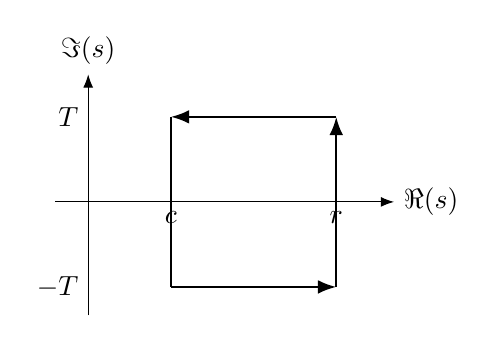
\begin{tikzpicture}[baseline={(current bounding box.center)}, >=Latex, x=1.05cm, y=0.9cm]
		\draw[->] (-0.4,0) -- (3.7,0) node[right] {$\Re(s)$};
		\draw[->] (0,-1.6) -- (0,1.8) node[above] {$\Im(s)$};
		\draw[thick, ->] (1,-1.2) -- (3,-1.2);
		\draw[thick, ->] (3,-1.2) -- (3,1.2);
		\draw[thick, ->] (3,1.2) -- (1,1.2);
		\draw[thick] (1,1.2) -- (1,-1.2);
		\node[below] at (1,0) {$c$};
		\node[below] at (3,0) {$r$};
		\node[left] at (0,1.2) {$T$};
		\node[left] at (0,-1.2) {$-T$};
	\end{tikzpicture}
	\]
	由 Cauchy 积分定理（Cauchy's integral theorem），由于 $y^s/s$ 在这个矩形内部没有极点，
	\[
		I_c(y,T)=
		\frac1{2\pi i}
		\left(
		\int_{c-iT}^{r-iT}
		+
		\int_{r-iT}^{r+iT}
		+
		\int_{r+iT}^{c+iT}
		\right)y^s\frac{ds}{s}.
	\]
	于是
	\[
	\begin{aligned}
		|I_c(y,T)|
		&\leq
		\frac1{2\pi}
		\left(
		\int_c^r\frac{y^\sigma}{T}\,d\sigma
		+
		\int_{-T}^T\frac{y^r}{r}\,dt
		+
		\int_c^r\frac{y^\sigma}{T}\,d\sigma
		\right)\\
		&=
		\frac1{2\pi}
		\left(
		\frac2T\left.\frac{y^\sigma}{\log y}\right|_{\sigma=c}^r
		+
		2T\frac{y^r}{r}
		\right).
	\end{aligned}
	\]
	因为 $0<y<1$，所以
	\[
		\frac{y^r}{r}\to 0,
		\qquad
		\frac{y^r}{|\log y|}\to 0
	\]
	当 $r\to+\infty$。因此
	\[
		|I_c(y,T)|
		\leq
		\frac1{\pi T}\frac{y^c}{|\log y|}.
	\]

	(b) 另一方面，我们要证明
	\[
		|I_c(y,T)|\leq y^c.
	\]
	令
	\[
		R=\sqrt{c^2+T^2},
	\]
	并令 $C$ 为以原点为圆心、半径为 $R$ 的圆。令 $\gamma^+$ 为 $C$ 上从 $c-iT$ 出发到 $c+iT$ 结束的逆时针路径：
	\[
	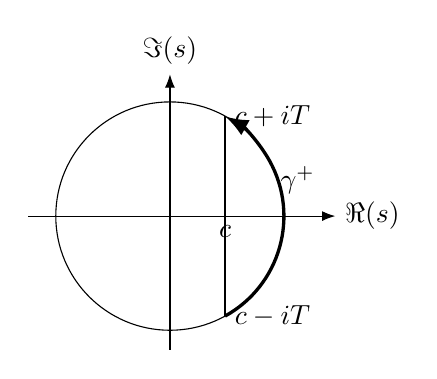
\begin{tikzpicture}[baseline={(current bounding box.center)}, >=Latex, x=1cm, y=1cm]
		\draw[->] (-1.8,0) -- (2.1,0) node[right] {$\Re(s)$};
		\draw[->] (0,-1.7) -- (0,1.8) node[above] {$\Im(s)$};
		\draw[thin] (0,0) circle (1.45);
		\draw[thick] (0.7,-1.27) -- (0.7,1.27);
		\draw[very thick, ->] (0.7,-1.27) arc[start angle=-61,end angle=61,radius=1.45];
		\node[right] at (0.7,1.27) {$c+iT$};
		\node[right] at (0.7,-1.27) {$c-iT$};
		\node[right] at (1.28,0.45) {$\gamma^+$};
		\node[below] at (0.7,0) {$c$};
	\end{tikzpicture}
	\]
	由 Cauchy 留数定理（Cauchy residue theorem），
	\[
		I_c(y,T)
		=
		\frac1{2\pi i}\int_{c-iT}^{c+iT}y^s\frac{ds}{s}
		=
		\frac1{2\pi i}\int_{\gamma^+}y^s\frac{ds}{s}.
	\]
	特别地，
	\[
		|I_c(y,T)|
		\leq
		\frac1{2\pi}\int_{\gamma^+}\frac{y^{\Re(s)}}{|s|}\,|ds|
		\leq
		\frac1{2\pi}\cdot \frac{y^c}{R}\cdot 2\pi R
		\leq y^c,
	\]
	这里用到了 $y<1$。

	\emph{情形 2：$y>1$。} 这时考虑如下矩形：
	\[
	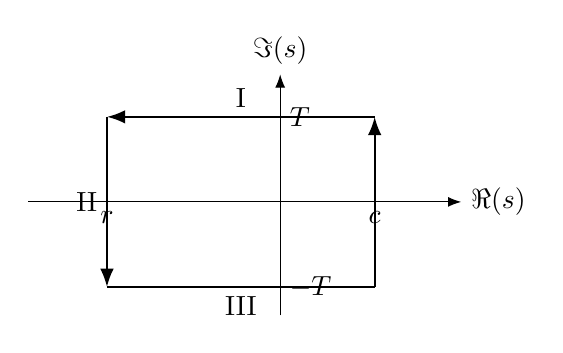
\begin{tikzpicture}[baseline={(current bounding box.center)}, >=Latex, x=1cm, y=0.9cm]
		\draw[->] (-3.2,0) -- (2.3,0) node[right] {$\Re(s)$};
		\draw[->] (0,-1.6) -- (0,1.8) node[above] {$\Im(s)$};
		\draw[thick, ->] (1.2,-1.2) -- (1.2,1.2);
		\draw[thick, ->] (1.2,1.2) -- (-2.2,1.2);
		\draw[thick, ->] (-2.2,1.2) -- (-2.2,-1.2);
		\draw[thick] (-2.2,-1.2) -- (1.2,-1.2);
		\node[below] at (1.2,0) {$c$};
		\node[below] at (-2.2,0) {$r$};
		\node[right] at (0,1.2) {$T$};
		\node[right] at (0,-1.2) {$-T$};
		\node[above] at (-0.5,1.2) {I};
		\node[left] at (-2.2,0) {II};
		\node[below] at (-0.5,-1.2) {III};
	\end{tikzpicture}
	\]
	由 Cauchy 留数定理，
	\[
		I_c(y,T)
		=
		\frac1{2\pi i}
		\left(
		\int_{\mathrm I}
		+
		\int_{\mathrm{II}}
		+
		\int_{\mathrm{III}}
		\right)y^s\frac{ds}{s}
		+
		\operatorname{Res}_{s=0}\frac{y^s}{s}.
	\]
	也就是说
	\[
		I_c(y,T)
		=
		1+
		\frac1{2\pi i}
		\left(
		\int_{\mathrm I}
		+
		\int_{\mathrm{II}}
		+
		\int_{\mathrm{III}}
		\right)y^s\frac{ds}{s}.
	\]
	和前面做同样的估计，并令 $r\to-\infty$，得到
	\[
		|I_c(y,T)-1|
		\leq
		\frac{2y^c}{1+T|\log y|}.
	\]
	结合两种估计，即得引理。
\end{proof}

\begin{theorem}[原文 Theorem 4.10，Perron 公式]
	设 $c>0$，$x,T\geq 1$ 为实数。设 $f\in\mathcal A$，且 $L_f(s)$ 在 $s=c$ 处绝对收敛。那么对所有 $x\notin\mathbb Z$，有
	\[
		\sum_{n\leq x}f(n)
		=
		\frac1{2\pi i}\int_{c-iT}^{c+iT}
		L_f(s)\frac{x^s}{s}\,ds
		+
		E(T),
	\]
	其中 $E(T)\to 0$ 当 $T\to\infty$。如果 $x\in\mathbb Z$，则公式也成立，只需把最后一项 $f(x)$ 替换为 $f(x)/2$。
\end{theorem}

\begin{proof}
	设 $x\notin\mathbb Z$。因为 $L_f(s)$ 在 $\Re(s)=c$ 上绝对收敛，所以可以交换求和与积分的次序：
	\[
	\begin{aligned}
		&\frac1{2\pi i}\int_{c-iT}^{c+iT}
		L_f(s)\frac{x^s}{s}\,ds\\
		&\qquad=
		\sum_{n\geq 1}f(n)
		\frac1{2\pi i}
		\int_{c-iT}^{c+iT}\left(\frac{x}{n}\right)^s\frac{ds}{s}.
	\end{aligned}
	\]
	由 Lemma 4.9，
	\[
		\frac1{2\pi i}\int_{c-iT}^{c+iT}
		L_f(s)\frac{x^s}{s}\,ds
		=
		\sum_{n\geq 1}f(n)\delta\left(\frac{x}{n}\right)
		+
		E(T),
	\]
	其中
	\[
	\begin{aligned}
		|E(T)|
		&\leq
		2\sum_{n\geq 1}
		\frac{|f(n)|(x/n)^c}
		{1+T|\log(x/n)|}\\
		&=
		2x^c\sum_{n\geq 1}
		\frac{|f(n)|}{n^c(1+T|\log(x/n)|)}.
	\end{aligned}
	\]
	由于 $\log(x/n)\neq 0$，所以 $|E(T)|\to 0$ 当 $T\to\infty$。因此
	\[
		\sum_{n\geq 1}f(n)\delta\left(\frac{x}{n}\right)
		=
		\sum_{n\leq x}f(n).
	\]
	$x\in\mathbb Z$ 的情形类似。
\end{proof}

\begin{remark}
	积分
	\[
		\frac1{2\pi i}\int_{c-i\infty}^{c+i\infty}
		L_f(s)\frac{x^s}{s}\,ds
	\]
	通常不是绝对收敛的，这会带来问题。在实践中，我们需要一个更实用的版本。
\end{remark}

\begin{theorem}[原文 Theorem 4.11，Perron 公式的截断版本]
	设 $c>0$，$x,T\geq 1$ 为实数。设 $f\in\mathcal A$，且 $L_f(s)$ 在 $s=c$ 处绝对收敛。那么对所有 $x\notin\mathbb Z$，有
	\[
		\sum_{n\leq x}f(n)
		=
		\frac1{2\pi i}\int_{c-iT}^{c+iT}
		L_f(s)\frac{x^s}{s}\,ds
		+
		O\left(
		x^c\sum_{n\geq 1}
		\frac{|f(n)|}{n^c(1+T|\log(x/n)|)}
		\right),
	\]
	其中误差项还满足
	\[
	\begin{aligned}
		x^c\sum_{n\geq 1}
		\frac{|f(n)|}{n^c(1+T|\log(x/n)|)}
		&\ll
		\frac{x^c}{T}\sum_{n\geq 1}\frac{|f(n)|}{n^c}\\
		&\quad+
		\left(1+\frac{x\log T}{T}\right)
		\max_{3x/4\leq n\leq 5x/4}|f(n)|.
	\end{aligned}
	\]
	如果 $x\in\mathbb Z$，则公式也成立，只需把最后一项 $f(x)$ 替换为 $f(x)/2$。
\end{theorem}

\begin{proof}
	Dirichlet 级数 $L_f(s)$ 在紧区间 $[c-iT,c+iT]$ 上绝对且一致收敛。因此
	\[
	\begin{aligned}
		\frac1{2\pi i}\int_{c-iT}^{c+iT}
		L_f(s)\frac{x^s}{s}\,ds
		&=
		\frac1{2\pi i}\int_{c-iT}^{c+iT}
		\sum_{n\geq 1}\frac{f(n)}{n^s}\frac{x^s}{s}\,ds\\
		&=
		\sum_{n\geq 1}f(n)
		\frac1{2\pi i}\int_{c-iT}^{c+iT}
		\left(\frac{x}{n}\right)^s\frac{ds}{s}\\
		&=
		\sum_{n\geq 1}f(n)I_c\left(\frac{x}{n},T\right)\\
		&=
		\sum_{n\geq 1}f(n)\delta\left(\frac{x}{n}\right)
		+
		\sum_{n\geq 1}f(n)
		\left(I_c\left(\frac{x}{n},T\right)
		-
		\delta\left(\frac{x}{n}\right)\right)\\
		&=
		\sum_{n\leq x}^{*}f(n)+E_c(x,T).
	\end{aligned}
	\]
	这里 $\sum_{n\leq x}^{*}$ 表示如果 $x\in\mathbb Z$，最后一项 $f(x)$ 替换为 $f(x)/2$。

	由 Lemma 4.9，
	\[
		|E_c(x,T)|
		\leq
		2\sum_{\substack{n\geq 1\\ n\neq x}}
		|f(n)|\frac{(x/n)^c}{1+T|\log(x/n)|}
		+
		\frac{c}{c+T}|f(x)|,
	\]
	其中最后一项只在 $x\in\mathbb Z$ 时出现。因此
	\[
		|E_c(x,T)|
		\leq
		2x^c\sum_{\substack{n\geq 1\\ n\neq x}}
		\frac{|f(n)|}{n^c(1+T|\log(x/n)|)}
		+
		\frac{c}{c+T}|f(x)|.
	\]
	特别地，
	\[
		|E_c(x,T)|\to 0
		\qquad (T\to\infty),
	\]
	于是得到 Theorem 4.10。

	现在把关于 $n$ 的和分成三部分：
	\[
		\sum_{|n-x|\geq x/4}(\cdots)
		+
		\sum_{2\leq |n-x|\leq x/4}(\cdots)
		+
		\sum_{|n-x|<2}(\cdots)
		=
		E_c^{(1)}(x,T)+E_c^{(2)}(x,T)+E_c^{(3)}(x,T).
	\]
	对满足 $|n-x|\geq x/4$ 的项，我们使用
	\[
		|\log(x/n)|\gg 1,
	\]
	它给出
	\[
		E_c^{(1)}(x,T)
		\ll
		\sum_{|n-x|\geq x/4}
		\frac{x^c|f(n)|}{n^cT|\log(x/n)|}
		\ll
		\frac{x^c}{T}\sum_{n\geq 1}\frac{|f(n)|}{n^c}.
	\]
	对满足 $2\leq |n-x|\leq x/4$ 的项，我们有
	\[
		|\log(x/n)|
		=
		\left|\log\left(1+\frac{n-x}{x}\right)\right|
		\gg
		\frac{|n-x|}{x}.
	\]
	所以
	\[
	\begin{aligned}
		E_c^{(2)}(x,T)
		&\ll
		\frac{x^c}{T}
		\sum_{2\leq |n-x|\leq x/4}
		\frac{|f(n)|x}{n^c|n-x|}\\
		&\ll
		\frac{x}{T}
		\left(\max_{2\leq |n-x|\leq x/4}|f(n)|\right)
		\sum_{2\leq |n-x|\leq x/4}\frac1{|n-x|}\\
		&\ll
		\frac{x\log x}{T}
		\max_{2\leq |n-x|\leq x/4}|f(n)|.
	\end{aligned}
	\]
	最后，剩下的项可以平凡地估计为
	\[
		E_c^{(3)}(x,T)
		\ll
		\sum_{|n-x|<2}\frac{x^c|f(n)|}{n^c}
		\ll
		\max_{|n-x|<2}|f(n)|.
	\]
	把这些估计相加即得定理。
\end{proof}

\chapter{指数、原根和指标}
\label{chap:indices-primitive-roots}

\weekmarker{第 7--8 周}

\section{指数和原根}

设 $n>1$，$(a,n)=1$，则由 Euler 定理知道
\[
	a^{\varphi(n)}\equiv 1\pmod n.
\]
所以，可能存在自然数 $d<\varphi(n)$，使得
\[
	a^d\equiv 1\pmod n.
\]

\begin{definition}[原文 定义 1]
	使得上式成立的最小正整数 $d$，称为 $a$ 模 $n$ 的次数（order），并称 $a$ 是属于指数 $d\pmod n$。我们把这个最小正整数 $d$ 记作 $\delta_n(a)$。为方便起见，当 $(a,n)\neq 1$ 时，令 $\delta_n(a)=0$。由 Euler 定理看出，
	\[
		\delta_n(a)\leq \varphi(n).
	\]
\end{definition}

\begin{definition}[原文 定义 2]
	若
	\[
		\delta_n(a)=\varphi(n),
	\]
	则 $a$ 称为模 $n$ 的原根（primitive root modulo $n$）。
\end{definition}

由定义知，对任意的 $\lambda<\delta_n(a)$，$a$ 不是同余方程
\[
	x^\lambda-1\equiv 0\pmod n
\]
的解。若 $a$ 是同余方程
\[
	x^d-1\equiv 0\pmod n
\]
的解，而对任一 $\lambda<d$，$a$ 不是同余方程
\[
	x^\lambda-1\equiv 0\pmod n
\]
的解，则称 $a$ 是方程
\[
	x^d-1\equiv 0\pmod n
\]
的原根。显然，这个方程的原根 $a$ 对模 $n$ 的次数为
\[
	\delta_n(a)=d.
\]
若 $a$ 是模 $n$ 的原根，则 $a$ 是
\[
	x^{\varphi(n)}-1\equiv 0\pmod n
\]
的原根。

我们现在可以从上述方程出发，而直接讨论指数、原根的性质。先来看几个例子。

\begin{example}[原文 例 1]
	求模 $7$ 的原根。

	此时 $n=7$，$\varphi(n)=6$，模 $7$ 的简化剩余系为
	\[
		1,2,3,4,5,6.
	\]
	列表如下：
	\[
	\begin{array}{c|cccccc}
		a & 1 & 2 & 3 & 4 & 5 & 6\\ \hline
		\delta_n(a) & 1 & 3 & 6 & 3 & 6 & 2
	\end{array}
	\]
	由此看出，$3,5$ 为模 $7$ 的全部原根。
\end{example}

\begin{example}[原文 例 2]
	求模 $15$ 的原根。

	此时 $n=15$，$\varphi(n)=8$，模 $15$ 的简化系为
	\[
		1,2,4,7,8,11,13,14.
	\]
	列表如下：
	\[
	\begin{array}{c|cccccccc}
		a & 1 & 2 & 4 & 7 & 8 & 11 & 13 & 14\\ \hline
		\delta_n(a) & 1 & 4 & 2 & 4 & 4 & 2 & 4 & 2
	\end{array}
	\]
	所以模 $15$ 无原根存在。
\end{example}

\begin{example}[原文 例 3]
	求模 $9$ 的原根。

	$n=9=3^2$，$\varphi(n)=6$，模 $9$ 的简化系为
	\[
		1,2,4,5,7,8.
	\]
	列表如下：
	\[
	\begin{array}{c|cccccc}
		a & 1 & 2 & 4 & 5 & 7 & 8\\ \hline
		\delta_n(a) & 1 & 6 & 3 & 6 & 3 & 2
	\end{array}
	\]
	所以 $2,5$ 为模 $9$ 的全部原根。
\end{example}

\begin{example}[原文 例 4]
	求模 $8$ 的原根。

	$n=8=2^3$，$\varphi(n)=4$，模 $8$ 的简化系为
	\[
		1,3,5,7.
	\]
	列表如下：
	\[
	\begin{array}{c|cccc}
		a & 1 & 3 & 5 & 7\\ \hline
		\delta_n(a) & 1 & 2 & 2 & 2
	\end{array}
	\]
	所以模 $8$ 不存在原根。
\end{example}

\begin{example}[原文 例 5]
	试证模 $n=2^k$，$k\geq 3$，必无原根。

	因为当 $n=2^k$ 时，
	\[
		\varphi(n)=2^{k-1},
	\]
	所以只需证明对于 $(a,2)=1$，必有
	\[
		a^{2^{k-2}}\equiv 1\pmod{2^k},
		\qquad k\geq 3.
	\]
	我们用归纳法证明。当 $k=3$，设 $a=2m+1$，则
	\[
		a^2=(2m+1)^2=4m(m+1)+1\equiv 1\pmod 8.
	\]
	若上述同余式对 $k_0\geq 3$ 成立，则当 $k=k_0+1$ 时，有
	\[
		a^{2^{k_0-1}}-1
		=
		\left(a^{2^{k_0-2}}-1\right)
		\left(a^{2^{k_0-2}}+1\right)
		\equiv 0\pmod{2^{k_0+1}}.
	\]
	证毕。
\end{example}

当 $n=2$ 时原根为 $1$，当 $n=4$ 时原根为 $3$。

下面来证明有关指数的一些基本性质。

\begin{theorem}[原文 定理 1]
	设
	\[
		a\equiv b\pmod n,
	\]
	则
	\[
		\delta_n(a)=\delta_n(b).
	\]
\end{theorem}

\begin{proof}
	证明是显然的。
\end{proof}

\begin{theorem}[原文 定理 2]
	同余式
	\[
		a^k\equiv 1\pmod n
	\]
	与
	\[
		\delta_n(a)\mid k
	\]
	等价。
\end{theorem}

\begin{proof}
	由 $\delta_n(a)\mid k$ 推出 $a^k\equiv 1\pmod n$ 是显然的。现假设 $a^k\equiv 1\pmod n$ 成立，令
	\[
		k=q\delta_n(a)+r,\qquad 0\leq r<\delta_n(a).
	\]
	若 $r\neq 0$，则得到
	\[
		a^k=a^{q\delta_n(a)}a^r,
	\]
	所以
	\[
		a^r\equiv a^k\equiv 1\pmod n.
	\]
	这与 $\delta_n(a)$ 为次数的定义矛盾，故必有 $r=0$。
\end{proof}

由上面两个定理可得到下面几个推论。

\begin{corollary}[原文 推论 1]
	\[
		\delta_n(a)\mid \varphi(n).
	\]
\end{corollary}

\begin{corollary}[原文 推论 2]
	设 $(a,n)=1$，则
	\[
		a^{k_1}\equiv a^{k_2}\pmod n
	\]
	与
	\[
		\delta_n(a)\mid (k_1-k_2)
	\]
	等价。
\end{corollary}

\begin{corollary}[原文 推论 3]
	设 $(a,n)=1$，则
	\[
		a^0,a^1,\ldots,a^{\delta_n(a)-1}
	\]
	模 $n$ 两两不同余。当 $a$ 为模 $n$ 的原根时，
	\[
		a^0,a^1,\ldots,a^{\delta_n(a)-1}
	\]
	组成模 $n$ 的简化系。
\end{corollary}

\begin{theorem}[原文 定理 3]
	设 $\lambda\mid \delta_n(a)$，则
	\[
		\delta_n(a^\lambda)=\frac{\delta_n(a)}{\lambda}.
	\]
\end{theorem}

\begin{proof}
	设 $\delta_n(a^\lambda)=d$。由于
	\[
		(a^\lambda)^{\delta_n(a)/\lambda}\equiv 1\pmod n,
	\]
	由定理 2 知
	\[
		d\mid \frac{\delta_n(a)}{\lambda}.
	\]
	若
	\[
		d<\frac{\delta_n(a)}{\lambda},
	\]
	则 $\lambda d<\delta_n(a)$，但
	\[
		a^{\lambda d}\equiv 1\pmod n,
	\]
	这与 $\delta_n(a)$ 的定义矛盾。所以 $\lambda d\geq \delta_n(a)$，因此必有
	\[
		d=\frac{\delta_n(a)}{\lambda}.
	\]
\end{proof}

\begin{theorem}[原文 定理 4]
	若 $(c,\delta_n(a))=1$，则
	\[
		\delta_n(a^c)=\delta_n(a).
	\]
\end{theorem}

\begin{proof}
	设 $\delta_n(a^c)=d$。由定理 2 知
	\[
		\delta_n(a)\mid cd.
	\]
	因为 $(\delta_n(a),c)=1$，所以
	\[
		\delta_n(a)\mid d.
	\]
	另一方面，又有
	\[
		(a^c)^{\delta_n(a)}\equiv 1\pmod n,
	\]
	由定理 2 知
	\[
		d\mid \delta_n(a).
	\]
	因此必有
	\[
		\delta_n(a)=d.
	\]
\end{proof}

\begin{theorem}[原文 定理 5]
	\[
		\delta_n(a^c)=\frac{\delta_n(a)}{(\delta_n(a),c)}.
	\]
\end{theorem}

\begin{proof}
	写
	\[
		a^c=a^{(c,\delta_n(a))\cdot c/(c,\delta_n(a))}.
	\]
	令
	\[
		b=a^{(c,\delta_n(a))}.
	\]
	由定理 3 知，$b$ 的次数为
	\[
		\frac{\delta_n(a)}{(c,\delta_n(a))}.
	\]
	又因为
	\[
		\left(\frac{c}{(c,\delta_n(a))},
		\frac{\delta_n(a)}{(c,\delta_n(a))}\right)=1,
	\]
	由定理 4 知 $a^c=b^{c/(c,\delta_n(a))}$ 的次数为
	\[
		\frac{\delta_n(a)}{(c,\delta_n(a))}.
	\]
\end{proof}

\begin{theorem}[原文 定理 6]
	若
	\[
		(\delta_n(a),\delta_n(b))=1,
	\]
	则
	\[
		\delta_n(ab)=\delta_n(a)\delta_n(b).
	\]
\end{theorem}

\begin{proof}
	设 $\delta_n(ab)=d$，则
	\[
		(ab)^d\equiv 1\pmod n.
	\]
	所以
	\[
		1\equiv (ab)^{d\delta_n(b)}\equiv a^{d\delta_n(b)}\pmod n.
	\]
	由此推出
	\[
		\delta_n(a)\mid d\delta_n(b).
	\]
	因为 $(\delta_n(a),\delta_n(b))=1$，故
	\[
		\delta_n(a)\mid d.
	\]
	同理，
	\[
		1\equiv (ab)^{d\delta_n(a)}\equiv b^{d\delta_n(a)}\pmod n,
	\]
	所以
	\[
		\delta_n(b)\mid d.
	\]
	因此
	\[
		\delta_n(a)\delta_n(b)\mid d.
	\]
	但显然有
	\[
		(ab)^{\delta_n(a)\delta_n(b)}\equiv 1\pmod n,
	\]
	所以
	\[
		d\mid \delta_n(a)\delta_n(b).
	\]
	必有
	\[
		d=\delta_n(a)\delta_n(b).
	\]
\end{proof}

条件 $(\delta_n(a),\delta_n(b))=1$ 不满足时，在一般情形下，并不能推出
\[
	\delta_n(ab)=[\delta_n(a),\delta_n(b)].
\]
现举例说明如下。设 $n=10$，简化系为
\[
	1,3,7,9.
\]
列表如下：
\[
\begin{array}{c|cccc}
	a & 1 & 3 & 7 & 9\\ \hline
	\delta_n(a) & 1 & 4 & 4 & 2
\end{array}
\]
得到
\[
\begin{aligned}
	\delta_n(3\times 3)
	&=\delta_n(9)=2\neq [\delta_n(3),\delta_n(3)]=4,\\
	\delta_n(3\times 7)
	&=\delta_n(1)=1\neq [\delta_n(3),\delta_n(7)]=4,\\
	\delta_n(3\times 9)
	&=\delta_n(7)=4=[\delta_n(3),\delta_n(9)]=4,\\
	\delta_n(7\times 9)
	&=\delta_n(3)=4=[\delta_n(7),\delta_n(9)]=4.
\end{aligned}
\]

\begin{theorem}[原文 定理 7]
	给定 $a,b$，存在 $c$，使得
	\[
		\delta_n(c)=[\delta_n(a),\delta_n(b)].
	\]
\end{theorem}

\begin{proof}
	显然只要证明 $(a,n)=(b,n)=1$ 的情形。

	令
	\[
		\delta=[\delta_n(a),\delta_n(b)]
		=
		q_1^{\alpha_1}q_2^{\alpha_2}\cdots q_s^{\alpha_s},
	\]
	这里 $q_i$，$1\leq i\leq s$，为素数。已知，对每个 $i$，有
	\[
		q_i^{\alpha_i}\mid \delta_n(a)
		\quad\text{或}\quad
		q_i^{\alpha_i}\mid \delta_n(b).
	\]
	设
	\[
		q_i^{\alpha_i}\mid \delta_n(a)
	\]
	成立，则有
	\[
		\delta_n(a)=q_i^{\alpha_i}\gamma_i.
	\]
	令
	\[
		c_i=a^{\gamma_i}.
	\]
	由定理 3 知
	\[
		\delta_n(c_i)=q_i^{\alpha_i}.
	\]
	这样我们证明了有
	\[
		c_1,c_2,\ldots,c_s
	\]
	存在，使得
	\[
		\delta_n(c_i)=q_i^{\alpha_i},
		\qquad 1\leq i\leq s.
	\]
	令
	\[
		c=c_1c_2\cdots c_s.
	\]
	由定理 6，得到
	\[
		\delta_n(c)=\delta_n(c_1)\delta_n(c_2)\cdots\delta_n(c_s)
		=
		q_1^{\alpha_1}q_2^{\alpha_2}\cdots q_s^{\alpha_s}
		=
		[\delta_n(a),\delta_n(b)].
	\]
\end{proof}

这个存在性定理的用处，可由下面情形看出。

\begin{theorem}[原文 定理 8]
	设 $(n_1,n_2)=1$，则
	\[
		\delta_{n_1n_2}(a)=[\delta_{n_1}(a),\delta_{n_2}(a)].
	\]
\end{theorem}

\begin{proof}
	设 $\delta_{n_1n_2}(a)=d$。显然
	\[
		a^d\equiv 1\pmod {n_1n_2}
	\]
	与
	\[
	\begin{cases}
		a^d\equiv 1\pmod {n_1},\\
		a^d\equiv 1\pmod {n_2}
	\end{cases}
	\]
	等价，所以
	\[
		\delta_{n_1}(a)\mid d,\qquad \delta_{n_2}(a)\mid d.
	\]
	由此推出
	\[
		[\delta_{n_1}(a),\delta_{n_2}(a)]\mid d.
	\]
	另一方面，
	\[
		a^{[\delta_{n_1}(a),\delta_{n_2}(a)]}\equiv 1\pmod {n_1},
	\]
	且
	\[
		a^{[\delta_{n_1}(a),\delta_{n_2}(a)]}\equiv 1\pmod {n_2}.
	\]
	所以
	\[
		a^{[\delta_{n_1}(a),\delta_{n_2}(a)]}\equiv 1\pmod {n_1n_2}.
	\]
	因此
	\[
		d\mid [\delta_{n_1}(a),\delta_{n_2}(a)].
	\]
	于是
	\[
		d=[\delta_{n_1}(a),\delta_{n_2}(a)].
	\]
\end{proof}

\begin{theorem}[原文 定理 9]
	设 $(n_1,n_2)=1$，则对给定的 $a_1,a_2$，必存在 $a$，使得
	\[
		\delta_{n_1n_2}(a)=[\delta_{n_1}(a_1),\delta_{n_2}(a_2)].
	\]
\end{theorem}

\begin{proof}
	考虑同余式组
	\[
	\begin{cases}
		x\equiv a_1\pmod {n_1},\\
		x\equiv a_2\pmod {n_2}.
	\end{cases}
	\]
	其解为
	\[
		x\equiv a\pmod {n_1n_2}.
	\]
	由定理 1 知
	\[
		\delta_{n_1}(a)=\delta_{n_1}(a_1),
		\qquad
		\delta_{n_2}(a)=\delta_{n_2}(a_2).
	\]
	由定理 8 得到
	\[
		\delta_{n_1n_2}(a)=[\delta_{n_1}(a_1),\delta_{n_2}(a_2)].
	\]
\end{proof}

\section{原根存在定理}

\begin{theorem}[原文 定理 10]
	设
	\[
		n=2^{\alpha_0}p_1^{\alpha_1}p_2^{\alpha_2}\cdots p_s^{\alpha_s},
	\]
	并令
	\[
		\varepsilon(n)
		=
		[\Phi(2^{\alpha_0}),\varphi(p_1^{\alpha_1}),\ldots,\varphi(p_s^{\alpha_s})],
	\]
	其中
	\[
		\Phi(2^{\alpha_0})
		=
		\begin{cases}
			\varphi(2^{\alpha_0}), & \alpha_0\leq 2,\\
			\varphi(2^{\alpha_0})/2, & \alpha_0\geq 3.
		\end{cases}
	\]
	则对任一 $a$，$(a,n)=1$，必有
	\[
		\delta_n(a)\mid \varepsilon(n).
	\]
\end{theorem}

\begin{proof}
	由定理 8 知
	\[
		\delta_n(a)
		=
		[\delta_{2^{\alpha_0}}(a),\delta_{p_1^{\alpha_1}}(a),\ldots,
		\delta_{p_s^{\alpha_s}}(a)].
	\]
	由定理 2 和例 5 知
	\[
		\delta_n(a)\mid \varepsilon(n).
	\]
\end{proof}

\begin{corollary}[原文 推论 4]
	当
	\[
		n\neq 2,4,p^\alpha,2p^\alpha\qquad (p>2)
	\]
	时，模 $n$ 不存在原根。
\end{corollary}

\begin{proof}
	因为由 $\varepsilon(n)$ 已知必有
	\[
		\varepsilon(n)\mid \varphi(n).
	\]
	当 $n$ 不是上述四种情形时，必有
	\[
		\varepsilon(n)\leq \frac12\varphi(n).
	\]
	因此这种 $n$，对任意 $(a,n)=1$，都有
	\[
		\delta_n(a)<\varphi(n).
	\]
	所以模 $n$ 无原根。
\end{proof}

当 $n=2,4,p^\alpha,2p^\alpha$ 时，原根存在。下面证明这一点。

\begin{lemma}[原文 引理 1]
	设素数 $p>2$。模 $p$ 存在原根。
\end{lemma}

\begin{proof}
	设 $1,2,\ldots,p-1$ 模 $p$ 的指数为
	\[
		\delta_p(1),\delta_p(2),\ldots,\delta_p(p-1).
	\]
	由定理 7 知，必有 $g$，使得
	\[
		\delta_p(g)=[\delta_p(1),\delta_p(2),\ldots,\delta_p(p-1)].
	\]
	因为
	\[
		g^{p-1}\equiv 1\pmod p,
	\]
	所以
	\[
		\delta_p(g)\mid (p-1).
	\]
	方程
	\[
		x^{\delta_p(g)}\equiv 1\pmod p
	\]
	有 $p-1$ 个解
	\[
		1,2,\ldots,p-1.
	\]
	于是 $p-1\leq \delta_p(g)$，必有
	\[
		\delta_p(g)=p-1.
	\]
	即 $g$ 为模 $p$ 的原根。
\end{proof}

\begin{lemma}[原文 引理 2]
	设 $\alpha\geq 2$。若 $g$ 是模 $p^\alpha$ 的原根，则 $g$ 也是模 $p^{\alpha-1}$ 的原根。
\end{lemma}

\begin{proof}
	设
	\[
		d=\delta_{p^{\alpha-1}}(g).
	\]
	要证
	\[
		d=\varphi(p^{\alpha-1}).
	\]
	因为
	\[
		g^d\equiv 1\pmod {p^{\alpha-1}},
	\]
	所以
	\[
		g^d=1+kp^{\alpha-1}.
	\]
	于是
	\[
		g^{dp}=(1+kp^{\alpha-1})^p=1+k'p^\alpha,
	\]
	所以
	\[
		g^{dp}\equiv 1\pmod {p^\alpha}.
	\]
	因为 $g$ 是模 $p^\alpha$ 的原根，所以
	\[
		\varphi(p^\alpha)\mid dp.
	\]
	因此
	\[
		\varphi(p^{\alpha-1})\mid d.
	\]
	另一方面，由 $d$ 的定义知
	\[
		d\mid \varphi(p^{\alpha-1}).
	\]
	所以必有
	\[
		d=\varphi(p^{\alpha-1}).
	\]
	这样，要找 $p^\alpha$ 的原根可以在 $p$ 中去找。
\end{proof}

\begin{lemma}[原文 引理 3]
	设 $g$ 为模 $p$ 的原根。存在 $t_0$，使得 $g+t_0p$ 是所有 $p^\alpha$，$\alpha\geq 1$，的原根。
\end{lemma}

\begin{proof}
	考虑 $g+tp$ 模 $p^2$ 的次数为 $\delta$。所以
	\[
		\delta\mid \varphi(p^2)=p(p-1).
	\]
	由于
	\[
		(g+tp)^\delta\equiv 1\pmod {p^2},
	\]
	所以
	\[
		(g+tp)^\delta\equiv 1\pmod p.
	\]
	但 $g$ 是模 $p$ 的原根，因此
	\[
		(p-1)\mid \delta.
	\]
	所以
	\[
		\delta=(p-1)p^r,
	\]
	这里 $r=0$ 或 $1$。我们只需取 $t_0$，使得 $r\neq 0$，即
	\[
		\delta=(p-1)p=\varphi(p^2).
	\]
	此时 $g+t_0p$ 为模 $p^2$ 的原根。下面来指出这种 $t_0$ 的存在性。

	有
	\[
		(g+tp)^{p-1}
		=
		g^{p-1}+(p-1)g^{p-2}tp+p^2T.
	\]
	因为
	\[
		g^{p-1}=1+T_1p,
	\]
	所以
	\[
		(g+tp)^{p-1}
		=
		1+p(T_1-g^{p-2}t)+p^2T_2.
	\]
	由上式看出，只要选取 $t_0$，使得
	\[
		g^{p-2}t_0\not\equiv T_1\pmod p,
	\]
	就有
	\[
		(g+t_0p)^{p-1}\not\equiv 1\pmod {p^2}.
	\]
	这推出 $g+t_0p$ 模 $p^2$ 的次数
	\[
		\delta=p(p-1).
	\]
	容易看出满足
	\[
		g^{p-2}t\equiv T_1\pmod p
	\]
	的 $t$ 只有一个，所以在其余 $p-1$ 个 $t\pmod p$ 中，上述条件都成立。

	所以我们可以用 $g$ 或 $g+p$ 去试算，取其中为模 $p^2$ 的原根者，则它是所有 $p^\alpha$，$\alpha\geq 1$，的原根。从上面的展开式容易看出，对于这样的 $t_0$，
	\[
		(g+t_0p)^{p-1}\not\equiv 1\pmod {p^2},
	\]
	所以它为模 $p^2$ 的原根；
	\[
		(g+t_0p)^{p(p-1)}\not\equiv 1\pmod {p^3},
	\]
	所以它为模 $p^3$ 的原根；依此类推，
	\[
		(g+t_0p)^{p^{\alpha-2}(p-1)}
		\not\equiv 1\pmod {p^\alpha},
	\]
	所以它为模 $p^\alpha$ 的原根。
\end{proof}

\begin{lemma}[原文 引理 4]
	设 $\alpha\geq 1$。若 $g$ 为模 $p^\alpha$，$p>2$，的原根，则 $g$ 和 $g+p^\alpha$ 中为奇数者是模 $2p^\alpha$ 的原根。
\end{lemma}

\begin{proof}
	因为 $g$ 和 $g+p^\alpha$ 均为模 $p^\alpha$ 的原根，设 $g$ 为奇数，则
	\[
		(g,2p^\alpha)=1.
	\]
	设 $g$ 对模 $2p^\alpha$ 的次数为 $d$。所以
	\[
		d\mid \varphi(2p^\alpha)=\varphi(p^\alpha).
	\]
	另一方面，从
	\[
		g^d\equiv 1\pmod {2p^\alpha}
	\]
	推出
	\[
		g^d\equiv 1\pmod {p^\alpha}.
	\]
	于是
	\[
		\varphi(p^\alpha)\mid d.
	\]
	因此必有
	\[
		d=\varphi(p^\alpha)=\varphi(2p^\alpha),
	\]
	即 $g$ 为模 $2p^\alpha$ 的原根。
\end{proof}

\begin{theorem}[原文 定理 11]
	当
	\[
		n=2,4,p^\alpha,2p^\alpha\qquad (p>2)
	\]
	时，模 $n$ 存在原根。
\end{theorem}

\begin{theorem}[原文 定理 12]
	若模 $n$ 存在原根，则模 $n$ 中次数为 $d$ 的数有 $\varphi(d)$ 个。特别地，模 $n$ 有
	\[
		\varphi(\varphi(n))
	\]
	个原根。
\end{theorem}

\begin{proof}
	因为 $g$ 为模 $n$ 的原根，所以
	\[
		g^0,g^1,\ldots,g^{\varphi(n)-1}
	\]
	为模 $n$ 的简化系。我们要在这 $\varphi(n)$ 个数中找出次数为 $d$ 的数。

	在
	\[
		g^\lambda,\qquad 0\leq \lambda\leq \varphi(n)-1,
	\]
	中，$g^\lambda$ 的次数为 $d$。由定理 5，得到
	\[
		\delta_n(g^\lambda)
		=
		\frac{\delta_n(g)}{(\delta_n(g),\lambda)}
		=
		\frac{\varphi(n)}{(\varphi(n),\lambda)}.
	\]
	所以 $\delta_n(g^\lambda)=d$ 的个数，等于满足
	\[
		(\varphi(n),\lambda)=\frac{\varphi(n)}{d}
	\]
	且 $0\leq \lambda\leq \varphi(n)-1$ 的 $\lambda$ 的个数。由上式看出，$\lambda$ 必有形式
	\[
		\lambda=\frac{\varphi(n)}{d}k,\qquad 0\leq k\leq d-1.
	\]
	于是
	\[
		\frac{\varphi(n)}{d}
		=
		\left(\varphi(n),\frac{\varphi(n)}{d}k\right)
		=
		\frac{\varphi(n)}{d}(d,k).
	\]
	因此 $k$ 必须满足
	\[
		(d,k)=1,\qquad 0\leq k\leq d-1.
	\]
	由此推出这样的 $k$ 有 $\varphi(d)$ 个，即这样的 $\lambda$ 有 $\varphi(d)$ 个。
\end{proof}

\section{\texorpdfstring{模 \(p^\alpha\)（\(p\geq 2\)）简化系的改造}{模 p alpha 简化系的改造}}

由前面知道，如果模 $n$ 有原根 $g$，则
\[
	g^0,g^1,\ldots,g^{\varphi(n)-1}
\]
为模 $n$ 的简化系。寻找模 $p$ 的原根通常称为一种“筛法”，事实如下：若 $a$ 模 $p$ 的次数为 $d$，且 $d<\varphi(p)$，则
\[
	a^1,a^2,\ldots,a^d
\]
都不可能为模 $p$ 的原根。

设模 $p$ 的简化系为
\[
	1,2,3,\ldots,p-1.
\]
首先取 $a=2$，其次数为 $d$。若 $d=p-1$，则 $2$ 为原根；若 $d<p-1$，则在上面的模 $p$ 数中将
\[
	2^1,2^2,\ldots,2^d
\]
删去。剩下 $\varphi(p-1)$ 个数为止，这些数全部为模 $p$ 的原根。

\begin{example}[原文 例 6]
	试求模 $41$ 的原根。

	模 $41$ 的简化系为
	\[
		1,2,3,\ldots,39,40.
	\]
	得 $2$ 的次数为 $20$，所以应消去与
	\[
		2^1,2^2,\ldots,2^{20}
	\]
	模 $41$ 同余的数。这些数为
	\[
	\begin{gathered}
		2,4,8,16,32,23,5,10,20,40,\\
		39,37,33,25,9,18,36,31,21,1.
	\end{gathered}
	\]
	因此，在模 $41$ 下剩下 $20$ 个数。但
	\[
		\varphi(40)=16<20,
	\]
	所以再来考虑 $3$。模 $41$ 下 $3$ 的次数为 $8$，所以应消去与
	\[
		3^1,3^2,\ldots,3^8
	\]
	模 $41$ 同余的数。这些数为
	\[
		3,9,27,40,38,32,14,1.
	\]
	其中 $1,9,32,40$ 这 $4$ 个数已被消去，这次只消去了 $4$ 个数。剩下的 $\varphi(40)$ 个数
	\[
	\begin{gathered}
		6,7,11,12,13,15,17,19,\\
		22,24,26,28,29,30,34,35
	\end{gathered}
	\]
	为模 $41$ 的原根。
\end{example}

模 $p$ 的原根找到以后，那么模 $p^\alpha$ 的原根都可以从
\[
	g^0,g^1,\ldots,g^{\varphi(n)-1}
\]
得到。至于 $n=2^\alpha$，$\alpha>2$，原根不存在时，其简化系应如何描述？

\begin{theorem}[原文 定理 13]
	设 $\alpha\geq 3$，则 $5$ 及 $3$ 对模 $2^\alpha$ 的次数为 $2^{\alpha-2}$，并且
	\[
		\pm 5^0,\pm 5^1,\ldots,\pm 5^{2^{\alpha-2}-1}
	\]
	及
	\[
		\pm 3^0,\pm 3^1,\ldots,\pm 3^{2^{\alpha-2}-1}
	\]
	均成模 $2^\alpha$ 的简化系。
\end{theorem}

\begin{proof}
	由例 5 知，当 $\alpha\geq 3$ 时，任一 $a$，$(a,2)=1$，有
	\[
		a^{2^{\alpha-2}}\equiv 1\pmod {2^\alpha}.
	\]
	所以任一 $a$ 的次数
	\[
		\delta_{2^\alpha}(a)\mid 2^{\alpha-2},
	\]
	为 $2^\lambda$ 的形式。下面来证明 $5$ 对模 $2^\alpha$ 的次数为 $2^{\alpha-2}$。

	当 $\alpha\geq 3$ 时，证明
	\[
		5^{2^{\alpha-3}}\not\equiv 1\pmod {2^\alpha}.
	\]
	当 $\alpha=3$ 时，由于
	\[
		5^{2^0}\not\equiv 1\pmod 8,
	\]
	所以结论成立。若结论对 $\alpha=k\geq 3$ 成立，则当 $\alpha=k+1$ 时也成立。事实上，当 $k\geq 3$ 时，有
	\[
		5^{2^{k-3}}\equiv 1\pmod {2^{k-1}}.
	\]
	设
	\[
		5^{2^{k-3}}=1+(2L+1)2^{k-1}.
	\]
	所以
	\[
		5^{2^{k-2}}
		=
		1+(2L+1)2^k+(2L+1)^2 2^{2k-2}.
	\]
	当 $k\geq 3$ 时，$2k-2\geq k+1$，所以由上式推出
	\[
		5^{2^{k-2}}\not\equiv 1\pmod {2^{k+1}}.
	\]
	这证明了上式当 $\alpha=k+1$ 时也成立。因此
	\[
		\delta_{2^\alpha}(5)=2^{\alpha-2},
		\qquad \alpha\geq 3.
	\]

	当 $\alpha\geq 3$ 时，
	\[
		\pm 5^0,\pm 5^1,\ldots,\pm 5^{2^{\alpha-2}-1}
	\]
	为模 $2^\alpha$ 的简化系。首先由 $\delta_{2^\alpha}(5)=2^{\alpha-2}$ 知
	\[
		5^0,5^1,5^2,\ldots,5^{2^{\alpha-2}-1}
	\]
	模 $2^\alpha$ 两两不同余；同样
	\[
		-5^0,-5^1,-5^2,\ldots,-5^{2^{\alpha-2}-1}
	\]
	模 $2^\alpha$ 两两不同余。其次，显然有
	\[
		5^{\alpha_1}\equiv 1\pmod 4,
		\qquad
		-5^{\alpha_2}\equiv -1\pmod 4.
	\]
	所以
	\[
		5^{\alpha_1}\not\equiv -5^{\alpha_2}\pmod 4.
	\]
	这证明了上面的数构成模 $2^\alpha$ 的简化系。同样，
	\[
		\pm 3^0,\pm 3^1,\ldots,\pm 3^{2^{\alpha-2}-1}
	\]
	也构成模 $2^\alpha$ 的简化系。
\end{proof}

\begin{theorem}[原文 定理 14]
	设 $n=2^\alpha$，$\alpha\geq 3$，则在模 $n$ 简化系中次数为 $d$ 的数的个数 $\psi(d)$ 为
	\[
		\psi(d)=
		\begin{cases}
			1, & d=1,\\
			3, & d=2,\\
			2\varphi(d), & d>2.
		\end{cases}
	\]
\end{theorem}

\begin{proof}
	由定理 13 知，当 $\alpha\geq 3$ 时，$1\leq a\leq 2^\alpha$ 且 $(a,2)=1$ 的简化系可由
	\[
		5^0,5^1,\ldots,5^{2^{\alpha-2}-1},
		-5^0,-5^1,\ldots,-5^{2^{\alpha-2}-1}
	\]
	表示。由定理 5 和定理 13 知
	\[
		\delta_{2^\alpha}(5^k)
		=
		\frac{\delta_{2^\alpha}(5)}{(\delta_{2^\alpha}(5),k)}
		=
		\frac{2^{\alpha-2}}{(2^{\alpha-2},k)}.
	\]
	和定理 12 相同，在
	\[
		5^0,5^1,\ldots,5^{2^{\alpha-2}-1}
	\]
	中次数为 $d$ 的数有 $\varphi(d)$ 个。在
	\[
		-5^0,-5^1,\ldots,-5^{2^{\alpha-2}-1}
	\]
	中，除了 $-5^0$ 的次数为 $2$ 外，$-5^k$，$1\leq k\leq 2^{\alpha-2}-1$，和 $5^k$ 的次数相同。所以有
	\[
		\psi(1)=1,\qquad
		\psi(2)=1+2\varphi(2),\qquad
		\psi(d)=2\varphi(d)\quad (d>2).
	\]
	并且容易验证
	\[
		\sum_{d\mid 2^{\alpha-2}}\psi(d)
		=
		1+1+2\sum_{\substack{d\mid 2^{\alpha-2}\\ d\geq 2}}\varphi(d)
		=
		2\sum_{d\mid 2^{\alpha-2}}\varphi(d)
		=
		2^{\alpha-1}.
	\]
\end{proof}

\begin{theorem}[原文 定理 15]
	设
	\[
		n=2^{\alpha_0}p_1^{\alpha_1}\cdots p_s^{\alpha_s},
	\]
	其中 $\varepsilon(n)$ 如定理 10 所给。存在 $a$，使得
	\[
		\delta_n(a)=\varepsilon(n).
	\]
\end{theorem}

\begin{proof}
	因为模 $p^\alpha$ 存在原根，次数为 $\varphi(p^\alpha)$；当 $\alpha_0\geq 3$ 时，$5$ 的次数为
	\[
		\Phi(2^{\alpha_0}),
	\]
	其中
	\[
		\Phi(2^{\alpha_0})
		=
		\begin{cases}
			\varphi(2^{\alpha_0}), & \alpha_0\leq 2,\\
			\frac12\varphi(2^{\alpha_0}), & \alpha_0>2.
		\end{cases}
	\]
	由定理 9 即得结论。
\end{proof}

为了解决任意模 $n$ 中这类问题，引入指标与指标组的概念。

\section{指标与指标组}

\begin{definition}[原文 定义 3]
	设 $n>1$，且模 $n$ 存在原根 $g$。对任一 $a$，$(a,n)=1$，存在 $r$，使得
	\[
		g^r\equiv a\pmod n,
		\qquad
		0\leq r\leq \varphi(n)-1.
	\]
	$r$ 称为以 $g$ 为底 $a$ 模 $n$ 的指标（index），记作
	\[
		\operatorname{ind}_{n,g}a
		=
		\operatorname{ind}_g a
		=
		\operatorname{ind} a.
	\]
\end{definition}

由定义看出，指标与原根 $g$ 有关。

下面列出基本性质。为方便起见，令
\[
	c=\varphi(n).
\]

\begin{theorem}[原文 定理 16]
	同余式
	\[
		g^{r'}\equiv a\pmod n
	\]
	与
	\[
		r'\equiv \operatorname{ind}a\pmod{\varphi(n)}
	\]
	等价。
\end{theorem}

\begin{proof}
	这是因为 $g$ 的次数为 $\varphi(n)$，由推论 2 即得。
\end{proof}

\begin{theorem}[原文 定理 17]
	\[
		\operatorname{ind}(a_1a_2)
		\equiv
		\operatorname{ind}a_1+\operatorname{ind}a_2
		\pmod c.
	\]
\end{theorem}

\begin{proof}
	由 $g$ 的定义和推论 2 得到上式。
\end{proof}

\begin{theorem}[原文 定理 18]
	\[
		\operatorname{ind}_{g_1}g_2\cdot \operatorname{ind}_{g_2}g_1
		\equiv 1\pmod c.
	\]
\end{theorem}

\begin{proof}
	设
	\[
		r_1=\operatorname{ind}_{g_1}g_2,
		\qquad
		r_2=\operatorname{ind}_{g_2}g_1.
	\]
	即
	\[
		g_1^{r_1}\equiv g_2\pmod n,
		\qquad
		g_2^{r_2}\equiv g_1\pmod n.
	\]
	所以
	\[
		g_2^{r_1r_2}\equiv g_2\pmod n.
	\]
	由推论 2 得到
	\[
		r_1r_2\equiv 1\pmod c.
	\]
	由此显然可推出
	\[
		(\operatorname{ind}_{g_1}g_2,c)=1.
	\]
\end{proof}

\begin{theorem}[原文 定理 19]
	\[
		\operatorname{ind}_{g_1}a
		\equiv
		\operatorname{ind}_{g_1}g_2\cdot\operatorname{ind}_{g_2}a
		\pmod c.
	\]
\end{theorem}

\begin{proof}
	有
	\[
		a\equiv g_2^{\operatorname{ind}_{g_2}a}
		\equiv
		g_1^{\operatorname{ind}_{g_1}g_2\cdot\operatorname{ind}_{g_2}a}
		\pmod n.
	\]
	由定理 16 得到结论。
\end{proof}

\begin{theorem}[原文 定理 20]
	设模 $n$ 的原根为 $g$，则
	\[
		\delta_n(a)=\frac{c}{(\operatorname{ind}_g a,c)}.
	\]
\end{theorem}

\begin{proof}
	因为
	\[
		\delta_n(g)=c,
		\qquad
		a\equiv g^{\operatorname{ind}_g a}\pmod n,
	\]
	由定理 5 得到
	\[
		\delta_n(a)=\frac{c}{(\operatorname{ind}_g a,c)}.
	\]
\end{proof}

公式 (35) 很方便。模 $p^\alpha$，$p>2$，存在原根；问题是，对于 $2^\alpha$，$\alpha\geq 3$，没有原根时，应如何处理？

\begin{definition}[原文 定义 4]
	设 $n=2^\alpha$，$\alpha\geq 3$。对任一 $a$，$(a,2)=1$，存在一对 $r_{-1}$ 和 $r_0$，满足
	\[
		0\leq r_{-1}<2,\qquad 0\leq r_0<2^{\alpha-2},
	\]
	使得
	\[
		a\equiv (-1)^{r_{-1}}5^{r_0}\pmod {2^\alpha}.
	\]
	$(r_{-1},r_0)$ 称为以 $-1,5$ 为底 $a$ 模 $2^\alpha$ 的指标组。
\end{definition}

当包含 $\alpha\leq 2$ 的情形时，为了记号方便，令
\[
	C_{-1}=
	\begin{cases}
		1, & \alpha=1,\\
		2, & \alpha\geq 2,
	\end{cases}
	\qquad
	C_0=
	\begin{cases}
		1, & \alpha=1,\\
		2^{\alpha-2}, & \alpha\geq 2.
	\end{cases}
\]

\begin{definition}[原文 定义 5]
	设 $n=2^\alpha$，$\alpha\geq 1$。对任一 $a$，$(a,2)=1$，存在一对 $r_{-1}$ 和 $r_0$，满足
	\[
		0\leq r_{-1}<C_{-1},
		\qquad
		0\leq r_0<C_0,
	\]
	使得
	\[
		a\equiv (-1)^{r_{-1}}5^{r_0}\pmod {2^\alpha}.
	\]
	$(r_{-1},r_0)$ 称为以 $-1,5$ 为底 $a$ 模 $2^\alpha$ 的指标组。
\end{definition}

下面列出基本性质。

\begin{theorem}[原文 定理 21]
	\[
		r_{-1}\equiv \frac{a-1}{2}\pmod {C_{-1}}.
	\]
\end{theorem}

\begin{proof}
	当 $\alpha\geq 3$ 时，$C_{-1}=2$。由前面同余可知，当
	\[
		a\equiv 1\pmod 4
	\]
	时，$r_{-1}=0$；当
	\[
		a\equiv -1\pmod 4
	\]
	时，$r_{-1}=1$。所以当 $\alpha\geq 3$ 时结论成立。当 $\alpha=1$ 时，$C_{-1}=1$，$C_0=1$；当 $\alpha=2$ 时，$C_0=1$，$C_{-1}=2$，验证即得。
\end{proof}

\begin{theorem}[原文 定理 22]
	同余式
	\[
		(-1)^{r'_{-1}}5^{r'_0}\equiv a\pmod {2^\alpha}
	\]
	与
	\[
		r'_{-1}\equiv r_{-1}\pmod {C_{-1}},
		\qquad
		r'_0\equiv r_0\pmod {C_0}
	\]
	等价。
\end{theorem}

\begin{proof}
	假定 $\alpha\geq 2$。此时 $C_{-1}=2$，由定理 21 知
	\[
		r'_{-1}\equiv r_{-1}\equiv \frac{a-1}{2}\pmod {C_{-1}}.
	\]
	所以只需证明第二个同余。由
	\[
		(-1)^{r'_{-1}}5^{r'_0}
		\equiv
		(-1)^{r_{-1}}5^{r_0}
		\pmod {2^\alpha}
	\]
	得到
	\[
		5^{r'_0}\equiv 5^{r_0}\pmod {2^\alpha}.
	\]
	由于
	\[
		\delta_{2^\alpha}(5)=C_0,
	\]
	因此由推论 2 得到
	\[
		r'_0\equiv r_0\pmod {C_0}.
	\]
\end{proof}

\begin{theorem}[原文 定理 23]
	设 $(a_1a_2,2)=1$，则
	\[
		r_{-1}(a_1a_2)
		\equiv
		r_{-1}(a_1)+r_{-1}(a_2)
		\pmod {C_{-1}},
	\]
	\[
		r_0(a_1a_2)
		\equiv
		r_0(a_1)+r_0(a_2)
		\pmod {C_0}.
	\]
\end{theorem}

\begin{proof}
	假定 $\alpha\geq 2$，此时 $C_{-1}=2$。第一个同余成立，因为
	\[
	\begin{aligned}
		\frac{a_1a_2-1}{2}
		&=
		\frac12\left(
		\left(1+2\cdot\frac{a_1-1}{2}\right)
		\left(1+2\cdot\frac{a_2-1}{2}\right)-1
		\right)\\
		&=
		\frac{a_1-1}{2}
		+
		\frac{a_2-1}{2}
		+
		\frac12(a_1-1)(a_2-1)\\
		&\equiv
		\frac{a_1-1}{2}
		+
		\frac{a_2-1}{2}
		\pmod 2.
	\end{aligned}
	\]
	由定理 21 得到第一个同余式。

	又由
	\[
		a_1a_2\equiv (-1)^{r_{-1}(a_1a_2)}5^{r_0(a_1a_2)}\pmod {2^\alpha},
	\]
	\[
		a_1\equiv (-1)^{r_{-1}(a_1)}5^{r_0(a_1)}\pmod {2^\alpha},
	\]
	\[
		a_2\equiv (-1)^{r_{-1}(a_2)}5^{r_0(a_2)}\pmod {2^\alpha},
	\]
	并注意 $C_{-1}=2$，可得
	\[
		5^{r_0(a_1a_2)}
		\equiv
		5^{r_0(a_1)}5^{r_0(a_2)}
		\pmod {2^\alpha}.
	\]
	由推论 2 并注意
	\[
		\delta_{2^\alpha}(5)=C_0,
	\]
	得到第二个同余式。
\end{proof}

模 $2^\alpha$ 选取的底不一定是 $-1$ 和 $5$。显然，只要任一 $g_0$ 模 $2^\alpha$ 的次数为 $2^{\alpha-2}$，则 $-1,g_0$ 构成模 $2^\alpha$ 的基。其他一些性质不在这里讨论。

\begin{theorem}[原文 定理 24]
	设
	\[
		n=2^{\alpha_0}p_1^{\alpha_1}\cdots p_s^{\alpha_s},
	\]
	并设 $g_1,\ldots,g_s$ 分别为模
	\[
		p_1^{\alpha_1},\ldots,p_s^{\alpha_s}
	\]
	的原根。给定一组数
	\[
		(r_{-1},r_0,r_1,\ldots,r_s),
	\]
	满足
	\[
		0\leq r_{-1}<C_{-1},\qquad
		0\leq r_0<C_0,
	\]
	以及
	\[
		0\leq r_i<C_i=\varphi(p_i^{\alpha_i}),
		\qquad 1\leq i\leq s.
	\]
	则存在一个 $a$，$(a,n)=1$，使得 $a$ 对 $2^{\alpha_0}$ 的指标组为 $(r_{-1},r_0)$，对 $p_i^{\alpha_i}$ 的指标为 $r_i$。当 $r_{-1},r_0,r_1,\ldots,r_s$ 遍历 $C_{-1},C_0,C_1,\ldots,C_s$ 的完全系时，$a$ 遍历模 $n$ 的简化系。
\end{theorem}

\begin{proof}
	考虑同余式组
	\[
	\begin{cases}
		x\equiv (-1)^{r_{-1}}5^{r_0}\pmod {2^{\alpha_0}},\\
		x\equiv g_1^{r_1}\pmod {p_1^{\alpha_1}},\\
		\cdots\\
		x\equiv g_s^{r_s}\pmod {p_s^{\alpha_s}}.
	\end{cases}
	\]
	它模 $n$ 的解为
	\[
		x\equiv a\pmod n.
	\]
	这就是所求。

	首先，$(a,n)=1$，已知 $a$ 满足要求。其次，只要
	\[
		r_{-1},r_0,r_1,\ldots,r_s
	\]
	和
	\[
		r'_{-1},r'_0,r'_1,\ldots,r'_s
	\]
	模 $C_{-1},C_0,C_1,\ldots,C_s$ 同余，则对应的解 $a,a'$ 模 $n$ 同余。当 $r_{-1},r_0,r_1,\ldots,r_s$ 遍历
	\[
		C_{-1},C_0,C_1,\ldots,C_s
	\]
	的完全系时，共得到
	\[
		C_{-1}C_0C_1\cdots C_s=\varphi(n)
	\]
	个 $a$，它们模 $n$ 两两不同余，且都与 $n$ 互素。反过来，若 $a$ 遍历模 $n$ 的简化系，则对应的
	\[
		r_{-1},r_0,r_1,\ldots,r_s
	\]
	也分别遍历相应的完全系。
\end{proof}

\section{二项同余方程}

设
\[
	n=2^{\alpha_0}p_1^{\alpha_1}\cdots p_s^{\alpha_s},
	\qquad
	k\geq 1,
	\qquad
	(a,n)=1.
\]
方程
\[
	x^k\equiv a\pmod n
\]
与方程组
\[
\begin{cases}
	x^k\equiv a\pmod {2^{\alpha_0}},\\
	x^k\equiv a\pmod {p_1^{\alpha_1}},\\
	\cdots\\
	x^k\equiv a\pmod {p_s^{\alpha_s}}
\end{cases}
\]
等价。

这类方程中，当 $n=p$，$k=2$ 时，前面已经讨论过。

\begin{theorem}[原文 定理 25]
	设 $n\geq 1$，模 $n$ 有原根 $g$，$(a,n)=1$，$k\geq 1$。则
	\[
		x^k\equiv a\pmod n
	\]
	有解，当且仅当
	\[
		(k,\varphi(n))\mid \operatorname{ind}a.
	\]
	若有解，则恰有 $(k,\varphi(n))$ 个解。
\end{theorem}

\begin{proof}
	设
	\[
		x=g^y,\qquad a=g^{\operatorname{ind}a}.
	\]
	则
	\[
		x^k\equiv a\pmod n
	\]
	与
	\[
		g^{ky}\equiv g^{\operatorname{ind}a}\pmod n
	\]
	等价。由推论 2 知，这又与
	\[
		ky\equiv \operatorname{ind}a\pmod{\varphi(n)}
	\]
	等价。而这个线性同余式有解，当且仅当
	\[
		(k,\varphi(n))\mid \operatorname{ind}a.
	\]
	若有解，则它有 $(k,\varphi(n))$ 个解。
\end{proof}

\begin{definition}[原文 定义 6]
	设 $k\geq 1$，$n>1$，$(a,n)=1$。若
	\[
		x^k\equiv a\pmod n
	\]
	有解，则称 $a$ 为模 $n$ 的 $k$ 次剩余。
\end{definition}

\begin{theorem}[原文 定理 26]
	设 $k\geq 1$，$n>1$，$(a,n)=1$，且模 $n$ 有原根。则 $a$ 是模 $n$ 的 $k$ 次剩余，当且仅当
	\[
		a^{\varphi(n)/(\varphi(n),k)}\equiv 1\pmod n,
	\]
	并且模 $n$ 的 $k$ 次剩余个数为
	\[
		\frac{\varphi(n)}{(\varphi(n),k)}.
	\]
\end{theorem}

\begin{proof}
	由定理 25 知，$a$ 是 $k$ 次剩余，当且仅当
	\[
		(k,\varphi(n))\mid \operatorname{ind}a.
	\]
	在
	\[
		g^0,g^1,\ldots,g^{\varphi(n)-1}
	\]
	中，指标能被 $(k,\varphi(n))$ 整除的数恰有
	\[
		\frac{\varphi(n)}{(k,\varphi(n))}
	\]
	个。

	下面证明同余判别式。因为
	\[
		a^{\varphi(n)/(k,\varphi(n))}\equiv 1\pmod n
	\]
	与
	\[
		\delta_n(a)\mid \frac{\varphi(n)}{(k,\varphi(n))}
	\]
	等价，而
	\[
		\delta_n(a)=\frac{\varphi(n)}{(\operatorname{ind}a,\varphi(n))}.
	\]
	所以它又与
	\[
		\frac{\varphi(n)}{(\operatorname{ind}a,\varphi(n))}
		\mid
		\frac{\varphi(n)}{(k,\varphi(n))}
	\]
	等价，即
	\[
		\frac{\varphi(n)}{(k,\varphi(n))}
		=
		\lambda\,
		\frac{\varphi(n)}{(\operatorname{ind}a,\varphi(n))}.
	\]
	这等价于
	\[
		(k,\varphi(n))\mid(\operatorname{ind}a,\varphi(n)),
	\]
	也等价于
	\[
		(k,\varphi(n))\mid \operatorname{ind}a.
	\]
\end{proof}

\begin{theorem}[原文 定理 27]
	设 $n=2^\alpha$，$\alpha\geq 3$，$2\nmid a$，并且
	\[
		a\equiv (-1)^{r_{-1}}5^{r_0}\pmod {2^\alpha}.
	\]
	对于二项同余方程
	\[
		x^k\equiv a\pmod {2^\alpha},
	\]
	当 $2\nmid k$ 时方程总有一个解；当 $2\mid k$ 时，方程有解的充要条件是
	\[
		r_{-1}=0,\qquad (k,2^{\alpha-2})\mid r_0.
	\]
	此时它有
	\[
		2(k,2^{\alpha-2})
	\]
	个解。
\end{theorem}

\begin{proof}
	设
	\[
		x\equiv (-1)^u5^v\pmod {2^\alpha}.
	\]
	则方程
	\[
		x^k\equiv a\pmod {2^\alpha}
	\]
	与
	\[
		(-1)^{ku}5^{kv}\equiv (-1)^{r_{-1}}5^{r_0}\pmod {2^\alpha}
	\]
	等价，而后者与方程组
	\[
		ku\equiv r_{-1}\pmod 2,\qquad
		kv\equiv r_0\pmod {2^{\alpha-2}}
	\]
	等价。

	当 $(k,2)=1$ 时，$u,v$ 都有唯一解。当 $2\mid k$ 时，首先必须有
	\[
		r_{-1}=0,
	\]
	所以此时 $u$ 有两个解
	\[
		u=0,1.
	\]
	而
	\[
		kv\equiv r_0\pmod {2^{\alpha-2}}
	\]
	有解，当且仅当
	\[
		(k,2^{\alpha-2})\mid r_0,
	\]
	且此时有 $(k,2^{\alpha-2})$ 个解。因此总共有
	\[
		2(k,2^{\alpha-2})
	\]
	个解。
\end{proof}

\begin{example}[原文 例 7]
	解方程
	\[
		x^9\equiv 6\pmod 7.
	\]
	设 $n=7$，$\varphi(n)=6$，原根 $g=3$。列表如下：
	\[
	\begin{array}{c|cccccc}
		a & 1 & 2 & 3 & 4 & 5 & 6\\ \hline
		\operatorname{ind}a & 6 & 2 & 1 & 4 & 5 & 3
	\end{array}
	\]
	令 $x=3^y$，则方程等价于
	\[
		3^{9y}\equiv 3^3\pmod 7.
	\]
	于是
	\[
		9y\equiv 3\pmod 6.
	\]
	故
	\[
		y=1,3,5.
	\]
	因此方程的解为
	\[
		x\equiv 3,6,5\pmod 7.
	\]
\end{example}

% Source: /Users/wangweiqiao/Downloads/数论基础, 潘承洞/数论基础, 潘承洞_170-192.pdf
% 原 PDF 页码 167--189。按原文顺序转写；少量衔接词与定理环境为排版需要加入。

\chapter{Dirichlet 特征}
\label{chap:dirichlet-characters}

类似于自然数列中的素数分布问题，我们可以讨论在算术（等差）数列中的素数分布。这个问题之所以重要，不仅由于它是经典的素数分布问题的推广，更由于它在许多著名的数论问题的研究中起着重要作用。研究这一问题的主要工具是 Dirichlet 所引进的一类称之为特征的完全可乘函数 $\chi(n)$，通常称为 Dirichlet 特征（Dirichlet character）。本章所讨论的特征均为 Dirichlet 特征。

\section{模为素数幂的特征的定义及其性质}

首先我们来定义以素数幂为模的特征。

设 $k=p^\alpha$，$p>2$，$\alpha\geq 1$，设 $g$ 是所有模 $p^\alpha$（即 $p$ 给定，$\alpha$ 任意）的最小正原根。若 $(n,k)=1$，令 $r=\operatorname{ind} n$，即
\[
	n\equiv g^r\pmod k.
\]
此处为方便起见，令
\[
	e(x)=e^{2\pi i x}.
\]

\begin{definition}[原文 定义 1]
	设 $k=p^\alpha$，$p>2$，$\alpha\geq 1$。定义在全体自然数 $n$ 上的函数
	\begin{equation}
		\chi(n)=\chi(n;k)=\chi(n;k,m)=
		\begin{cases}
			0, & (n,k)>1,\\
			e\left(\dfrac{m\operatorname{ind}n}{\varphi(k)}\right), & (n,k)=1
		\end{cases}
		\tag{1}
	\end{equation}
	称为模 $k$ 的特征，这里参数 $m$ 为整数。
\end{definition}

由定义可看出，对同一个 $k$，特征关于 $m$ 是周期函数，周期为 $\varphi(k)$，所以对应于模 $k$ 的全部特征可由
\[
	m=0,1,\ldots,\varphi(k)-1
\]
得到。

再设 $k=2^\alpha$。当 $\alpha\geq 3$ 时，模 $k$ 没有原根。但对任一奇数 $n$，可引进指标组，即
\[
	n\equiv (-1)^{r_{-1}}5^{r_0}\pmod {2^\alpha}.
\]

\begin{definition}[原文 定义 2]
	设 $k=2^\alpha$，$\alpha\geq 1$。由下列公式给出定义在全体自然数 $n$ 上的函数，称为模 $k$ 的特征：
	\begin{equation}
		\chi(n)=\chi(n;2)=\chi(n;2,0,0)=
		\begin{cases}
			0, & (n,2)>1,\\
			1, & (n,2)=1;
		\end{cases}
		\tag{2}
	\end{equation}
	\begin{equation}
		\chi(n)=\chi(n;4)=\chi(n;4,m_{-1},0)=
		\begin{cases}
			0, & (n,2)>1,\\
			(-1)^{m_{-1}r_{-1}}, & (n,2)=1,
		\end{cases}
		\tag{3}
	\end{equation}
	这里 $n\equiv (-1)^{r_{-1}}\pmod 4$，参数 $m_{-1}$ 为整数；当 $\alpha\geq 3$ 时，
	\begin{equation}
		\chi(n)=\chi(n;2^\alpha)=\chi(n;2^\alpha,m_{-1},m_0)=
		\begin{cases}
			0, & (n,2)>1,\\
			(-1)^{m_{-1}r_{-1}}e\left(\dfrac{m_0r_0}{2^{\alpha-2}}\right), & (n,2)=1,
		\end{cases}
		\tag{4}
	\end{equation}
	这里参数 $m_{-1},m_0$ 为整数。
\end{definition}

由定义及指标的性质可得到下面的定理。

\begin{theorem}[原文 定理 1]
	设 $k=p^\alpha$，$p\geq 2$，$\alpha\geq 1$，则有
	\[
	\begin{cases}
		\chi(n;p^\alpha)=0, & (n,p)>1,\\
		|\chi(n;p^\alpha)|=1, & (n,p)=1,\\
		\chi(1;p^\alpha)=1;
	\end{cases}
	\]
	$\chi(n;p^\alpha)$ 是 $n$ 的周期函数，周期为 $p^\alpha$；并且 $\chi(n;p^\alpha)$ 是 $n$ 的完全可乘函数，即
	\[
		\chi(n_1n_2;p^\alpha)=\chi(n_1;p^\alpha)\chi(n_2;p^\alpha).
	\]
\end{theorem}

\begin{theorem}[原文 定理 2]
	对每一个模 $k=p^\alpha$，$p\geq 2$，$\alpha\geq 1$，恰好有 $\varphi(k)$ 个不同的特征。
\end{theorem}

\begin{proof}
	首先设 $k=p^\alpha$，$p>2$，$\alpha\geq 1$。由定义 1 知，模 $k$ 的所有特征由
	\[
		m=0,1,2,\ldots,\varphi(k)-1
	\]
	得到，故只要证明这 $\varphi(k)$ 个特征两两不相同。

	设 $0\leq m,m'<\varphi(k)$，$m\neq m'$。若
	\[
		\chi(n;k,m)=\chi(n;k,m'),
	\]
	则由定理 1 的第一部分及当 $n$ 遍历模 $k$ 的简化系时其指标 $r$ 遍历模 $\varphi(k)$ 的完全系，得到
	\[
	\begin{aligned}
		\varphi(k)
		&=
		\sum_{\substack{1\leq n\leq k\\ (n,k)=1}}
		\chi(n;k,m)\overline{\chi(n;k,m')}  \\
		&=
		\sum_{r=0}^{\varphi(k)-1}
		e\left(\frac{(m-m')r}{\varphi(k)}\right)
		=0.
	\end{aligned}
	\]
	这矛盾。因此对 $k=p^\alpha$，$p>2$ 的情形已经证明。

	现在设 $k=2^\alpha$，$\alpha\geq 3$。由定义 2 知，$m_{-1},m_0$ 和 $m_{-1}+2,m_0+2^{\alpha-2}$ 对应同一个特征，所以模 $k$ 的所有特征由
	\[
		m_{-1}=0,1,\qquad m_0=0,1,\ldots,2^{\alpha-2}-1
	\]
	给出，共有 $2\cdot 2^{\alpha-2}=\varphi(2^\alpha)$ 个。因此只要证明这些特征两两不相同。

	用反证法。设
	\[
		0\leq m_{-1},m'_{-1}<2,\qquad
		0\leq m_0,m'_0<2^{\alpha-2},
	\]
	且 $m_{-1}=m'_{-1}$、$m_0=m'_0$ 不能同时成立。若
	\[
		\chi(n;k,m_{-1},m_0)=\chi(n;k,m'_{-1},m'_0),
	\]
	则由定理 1 的第一部分及当 $n$ 遍历模 $k$ 的简化系时其指标组 $r_{-1},r_0$ 分别遍历模 $2$ 及 $2^{\alpha-2}$ 的完全系，得到
	\[
	\begin{aligned}
		\varphi(2^\alpha)
		&=
		\sum_{\substack{1\leq n\leq 2^\alpha\\ (n,2)=1}}
		\chi(n;k,m_{-1},m_0)\overline{\chi(n;k,m'_{-1},m'_0)}  \\
		&=
		\sum_{r_{-1}=0}^{1}(-1)^{r_{-1}(m_{-1}-m'_{-1})}
		\sum_{r_0=0}^{2^{\alpha-2}-1}
		e\left(\frac{(m_0-m'_0)r_0}{2^{\alpha-2}}\right)
		=0.
	\end{aligned}
	\]
	上式最后一步用到了对参数的限制。矛盾，于是 $k=2^\alpha$，$\alpha\geq 3$ 的情形也得证。

	最后，当 $k=2$ 时只有 $1$ 个特征；当 $k=4$ 时有 $2$ 个不同特征。因此定理全部得证。
\end{proof}

我们把下面的特征称为主特征（principal character）：
\begin{equation}
	\chi_0(n;k)=
	\begin{cases}
		0, & (n,k)>1,\\
		1, & (n,k)=1.
	\end{cases}
	\tag{5}
\end{equation}
主特征可简记为 $\chi_0(n;k)=\chi_0(n)=\chi_0$。

\begin{theorem}[原文 定理 3，正交性]
	设 $k=p^\alpha$，$p\geq 2$，$\alpha\geq 1$，则有
	\begin{equation}
		\frac{1}{\varphi(k)}\sum_{\chi\bmod k}\chi(n)
		=
		\begin{cases}
			1, & n\equiv 1\pmod k,\\
			0, & n\not\equiv 1\pmod k,
		\end{cases}
		\tag{6}
	\end{equation}
	这里的求和号表示对模 $k$ 的所有 $\varphi(k)$ 个特征求和，并且
	\begin{equation}
		\frac{1}{\varphi(k)}\sum_{n=1}^{k}\chi(n)
		=
		\begin{cases}
			1, & \chi=\chi_0,\\
			0, & \chi\neq\chi_0.
		\end{cases}
		\tag{6'}
	\end{equation}
\end{theorem}

\begin{proof}
	我们只证明式 \((6)\) 的第二个式子。以 $p>2$ 的情形为例，当 $n\not\equiv1\pmod k$ 时，$\operatorname{ind}n\not\equiv0\pmod{\varphi(k)}$，故
	\[
		\sum_{\chi\bmod k}\chi(n)
		=
		\sum_{m=0}^{\varphi(k)-1}
		e\left(\frac{m\operatorname{ind}n}{\varphi(k)}\right)
		=0.
	\]
	模 $2^\alpha$ 的情形同理使用指标组，其他几个式子可从定义直接推出。
\end{proof}

特征 $\chi(n)$ 的一个重要性质是周期性。对模 $k$ 的特征来说，$k$ 当然是它的周期，但是特征可以有小于 $k$ 的周期。例如对模 $k=p^\alpha$、$\alpha>1$ 来说，显有
\[
	\chi_0(n;p^\alpha)=\chi_0(n;p),
\]
因此
\[
	\chi_0(n+p;p^\alpha)=\chi_0(n;p^\alpha).
\]
所以，对每一个模 $k$ 的特征 $\chi(n;k)$，一定有一个最小正周期 $e$；利用带余数除法很容易证明 $e\mid k$。我们把非主特征中最小正周期恰好等于其模的特征称为原特征（primitive character），其他的称为非原特征（imprimitive character）。这样模 $k$ 的特征就被分为原特征、非原特征两类，而最重要的是原特征。显然，模 $p$（$p>2$）的非主特征均为原特征，模 $2$ 没有原特征，模 $4$ 的原特征为 $\chi(n;4,1,0)$。

\begin{theorem}[原文 定理 4]
	设 $k=p^\alpha$，$p>2$，则 $\chi(n;p^\alpha,m)$ 是原特征的充要条件为
	\[
		(m,p)=1.
	\]
	当 $k=2^\alpha$，$\alpha\geq 3$ 时，$\chi(n;2^\alpha,m_{-1},m_0)$ 为原特征的充要条件为
	\[
		(m_0,2)=1.
	\]
\end{theorem}

\begin{proof}
	设 $k=p^\alpha$，$p>2$。先证必要性。设
	\[
		\chi(n;p^\alpha,m)
		=
		e\left(\frac{m\operatorname{ind}n}{\varphi(p^\alpha)}\right),
		\qquad 0<m<\varphi(p^\alpha),
	\]
	为非主特征。若 $(m,p)>1$，则可写
	\[
		m=m'p^\beta,\qquad (m',p)=1,\qquad 1\leq\beta<\alpha.
	\]
	于是
	\[
		\chi(n;p^\alpha,m)
		=
		e\left(\frac{m'\operatorname{ind}n}{\varphi(p^{\alpha-\beta})}\right)
		=
		\chi(n;p^{\alpha-\beta},m').
	\]
	这与原特征的定义矛盾，所以必有 $(m,p)=1$。

	再证充分性。因为对模 $k=p$ 来说，$(n,p)=1$ 时的非主特征均为原特征。现设 $k=p^\alpha$，$\alpha>1$。由于最小正周期 $e\mid k$，我们只要证明当 $(m,p)=1$ 时，模 $k$ 的非主特征对任意 $1\leq\lambda<\alpha$ 不可能以模 $p^\lambda$ 为其周期。取 $n=1+p^\lambda$。显然 $n\equiv1\pmod {p^\lambda}$，但 $n\not\equiv1\pmod {p^{\lambda+1}}$。若 $r=\operatorname{ind}n$，则指标的性质给出
	\[
		r\equiv0\pmod {\varphi(p^\lambda)},\qquad
		r\not\equiv0\pmod {\varphi(p^{\lambda+1})}.
	\]
	于是可写
	\[
		r=a\varphi(p^\lambda),\qquad p\nmid a.
	\]
	因为 $(m,p)=1$，所以
	\[
		\frac{m\operatorname{ind}n}{\varphi(p^\alpha)}
		=
		\frac{ma}{p^{\alpha-\lambda}}
	\]
	不是整数，从而
	\[
		\chi(n;p^\alpha,m)\neq1=\chi(1;p^\alpha,m).
	\]
	因此 $p^\lambda$ 不是周期，故该特征为原特征。

	下面证明 $k=2^\alpha$ 的情形。当 $k=2$ 时，仅有一个主特征 $\chi_0(n;2)$；当 $k=4$ 时，非主特征为 $\chi(n;4,1,0)$，因为 $\chi(3;4,1,0)=-1$，所以它是原特征。

	当 $\alpha\geq 3$ 时，非主特征为
	\[
		\chi(n;2^\alpha,m_{-1},m_0)
		=
		(-1)^{m_{-1}r_{-1}}
		e\left(\frac{m_0r_0}{2^{\alpha-2}}\right),
		\qquad (n,2)=1,
	\]
	这里参数 $m_{-1},m_0$ 满足
	\[
		0\leq m_{-1}<2,\qquad 0\leq m_0<2^{\alpha-2},
	\]
	且 $m_{-1},m_0$ 不同时为 $0$。

	先证必要性。若 $(m_0,2)>1$，当 $m_0=0$ 时必有 $m_{-1}=1$，此时
	\[
		\chi(n;2^\alpha,m_{-1},m_0)=\chi(n;4,1,0),
	\]
	因为 $\alpha\geq3$，这和 $\chi$ 为原特征矛盾。若 $m_0>0$，则可写
	\[
		m_0=m'_0\,2^\beta,\qquad 1\leq\beta<\alpha-2,\qquad (m'_0,2)=1.
	\]
	由指标组性质知，当 $n\equiv n'\pmod {2^{\alpha-\beta}}$ 且 $(n,2)=1$ 时，
	\[
		r_{-1}(n)\equiv r_{-1}(n')\pmod 2,\qquad
		r_0(n)\equiv r_0(n')\pmod {2^{\alpha-\beta-2}}.
	\]
	于是 $\chi$ 有小于 $2^\alpha$ 的周期，矛盾。因此必有 $(m_0,2)=1$。

	再证充分性。若 $(m_0,2)=1$，则对任意 $2\leq\lambda<\alpha$，取 $n=1+2^\lambda$。显然 $n\not\equiv1\pmod {2^\alpha}$，且由指标组性质可得
	\[
		r_{-1}(n)=0,\qquad r_0(n)\not\equiv0\pmod {2^{\alpha-2}}.
	\]
	于是
	\[
		\chi(n;2^\alpha,m_{-1},m_0)\neq1.
	\]
	故任意 $2^\lambda$（$\lambda<\alpha$）均不为其周期，所以它是原特征。
\end{proof}

\begin{theorem}[原文 定理 5]
	设 $k=p^\alpha$，$p\geq 2$。对模 $k$ 的每一个非主特征，必有唯一的一个模 $k^*=p^\lambda$（$\lambda\leq\alpha$）及唯一的一个模 $k^*$ 的原特征与它恒等。反过来，对模 $k^*=p^\lambda$ 的每一个原特征，对每一个模 $k=p^\alpha$（$\alpha\geq\lambda$），必有唯一的一个模 $k$ 的非主特征与它恒等。
\end{theorem}

\begin{proof}
	先证 $k=p^\alpha$，$p>2$ 的情形。若 $\chi(n;p^\alpha,m)$ 是原特征，则取 $k^*=p^\alpha$，所得原特征就是它自身。若它是非原特征，则必有 $\alpha\geq2$，$0<m<\varphi(p^\alpha)$，且 $(m,p)>1$。于是可写
	\[
		m=m'p^\beta,\qquad 1\leq\beta<\alpha,\qquad (m',p)=1.
	\]
	由式 \((1)\) 得
	\[
		\chi(n;p^\alpha,m)=\chi(n;p^{\alpha-\beta},m'),
	\]
	而由定理 4 知右边为模 $p^{\alpha-\beta}$ 的原特征。唯一性由原特征的定义推出。反过来，当 $\alpha=\lambda$ 时取原特征自身；当 $\alpha>\lambda$ 时，只要取 $m$ 为相应参数乘以 $p^{\alpha-\lambda}$ 即可。

	下面证明 $k=2^\alpha$ 的情形。若 $\chi(n;2^\alpha,m_{-1},m_0)$ 为原特征，则取 $k^*=2^\alpha$，所得原特征就是它自身。若它为非原特征，则必有 $\alpha\geq3$ 且 $(m_0,2)>1$。当 $m_0=0$ 时，必有 $m_{-1}=1$，而
	\[
		\chi(n;2^\alpha,1,0)=\chi(n;4,1,0),
	\]
	即为对应模 $4$ 的原特征。当 $m_0>0$ 时，可写
	\[
		m_0=m'_0\,2^\beta,\qquad 1\leq\beta<\alpha-2,\qquad (m'_0,2)=1.
	\]
	由特征定义及指标组性质知
	\[
		\chi(n;2^\alpha,m_{-1},m_0)
		=
		\chi(n;2^{\alpha-\beta},m_{-1},m'_0),
	\]
	而右边为模 $2^{\alpha-\beta}$ 的原特征。反过来，当 $\alpha=\lambda$ 时取原特征自身；当 $\alpha>\lambda$ 时，模 $4$ 的原特征对应于模 $2^\alpha$（$\alpha\geq3$）的非原特征 $\chi(n;2^\alpha,1,0)$；模 $2^\lambda$（$\lambda>2$）的原特征 $\chi(n;2^\lambda,m_{-1},m_0)$ 对应于模 $2^\alpha$ 的非原特征
	\[
		\chi(n;2^\alpha,m_{-1},m_0\,2^{\alpha-\lambda}).
	\]
	定理得证。
\end{proof}

仅取实值的特征称为实特征（real character），其他称为复特征（complex character），主特征显然为实特征。

\begin{theorem}[原文 定理 6]
	设 $k=p^\alpha$，$p>2$，则 $\chi(n;p^\alpha,m)$ 为实特征的充要条件是
	\[
		m\equiv0,\ \frac{1}{2}\varphi(p^\alpha)\pmod{\varphi(p^\alpha)}.
	\]
	模 $2$、模 $4$ 的特征均为实特征。当 $k=2^\alpha$（$\alpha\geq3$）时，$\chi(n;2^\alpha,m_{-1},m_0)$ 为实特征的充要条件为
	\[
		m_0\equiv0,\ 2^{\alpha-3}\pmod {2^{\alpha-2}}.
	\]
\end{theorem}

\begin{proof}
	由特征的定义可直接推出定理的论断。
\end{proof}

\begin{theorem}[原文 定理 7]
	设 $k=p^\alpha$，那么当且仅当模 $k=4,8$ 及 $p$（$p>2$）时，才有实原特征存在。
\end{theorem}

\begin{proof}
	当 $k=2$ 时无原特征。$k=4$ 时其非主特征为
	\[
		\chi(n;4,1,0)=
		\begin{cases}
			0, & (n,2)>1,\\
			(-1)^{(n-1)/2}, & (n,2)=1,
		\end{cases}
	\]
	显然为实原特征。

	当 $k=2^\alpha$，$\alpha\geq3$ 时，由定理 6 知，仅当 $m_0=2^{\alpha-3}$ 时才是实的非主特征；由定理 4 又知，仅当 $(m_0,2)=1$ 时才为原特征，所以一定有 $\alpha=3$，即 $k=8$。此时有两个实原特征：
	\[
		\chi(n;8,0,1),\qquad \chi(n;8,1,1),
	\]
	且
	\[
		\chi(n;8,0,1)=
		\begin{cases}
			0, & (n,2)>1,\\
			(-1)^{r_0}, & (n,2)=1,
		\end{cases}
	\]
	其中 $n\equiv5^{r_0}\pmod 8$，并且
	\[
		\chi(n;8,1,1)=\chi(n;4,1,0)\chi(n;8,0,1).
	\]

	当 $k=p^\alpha$，$p>2$ 时，由定理 6 知，仅当 $m=\frac{1}{2}\varphi(p^\alpha)$ 时才是实的非主特征；由定理 4 知，只有当 $(m,p)=1$ 时才是原特征，故必有 $\alpha=1$。于是实原特征为
	\[
		\chi\left(n;p,\frac{p-1}{2}\right)
		=
		(-1)^{\operatorname{ind}n}
		=
		\left(\frac{n}{p}\right),
	\]
	这里 $\left(\frac{n}{p}\right)$ 为 Legendre 符号（Legendre symbol）。因为原根一定是二次非剩余，所以若 $n\equiv g^r\pmod p$，则
	\[
		\left(\frac{n}{p}\right)
		=
		\left(\frac{g^r}{p}\right)
		=
		\left(\frac{g}{p}\right)^r
		=
		(-1)^r.
	\]
	定理得证。
\end{proof}

以上我们定义了以素数幂为模的特征，并讨论了它们的基本性质。下面我们来定义任意正整数 $k$（$k\geq2$）为模的特征，并把以上的定理推广到任意模的情形。

\section{任意模的特征的定义及其性质}

\begin{definition}[原文 定义 3]
	设 $k\geq2$，其标准分解式为
	\[
		k=p_1^{\alpha_1}p_2^{\alpha_2}\cdots p_s^{\alpha_s}.
	\]
	由等式
	\begin{equation}
		\chi(n)=\chi(n;k)=\prod_{j=1}^{s}\chi(n;p_j^{\alpha_j})
		\tag{7}
	\end{equation}
	所确定的函数 $\chi(n)$ 称为模 $k$ 的特征。这里 $\chi(n;p_j^{\alpha_j})$ 为以素数幂 $p_j^{\alpha_j}$ 为模的特征。
\end{definition}

不难看出，定理 1 对一般模的特征也是成立的。

\begin{theorem}[原文 定理 \(1'\)]
	设 $\chi(n;k)$ 为模 $k$ 的特征，则有
	\[
	\begin{cases}
		\chi(n;k)=0, & (n,k)>1,\\
		|\chi(n;k)|=1, & (n,k)=1,\\
		\chi(1;k)=1;
	\end{cases}
	\]
	并且
	\[
		\chi(n+k;k)=\chi(n;k),\qquad
		\chi(n_1n_2;k)=\chi(n_1;k)\chi(n_2;k).
	\]
\end{theorem}

\begin{theorem}[原文 定理 8]
	对每一个模 $k$，恰好有 $\varphi(k)$ 个不同的特征。
\end{theorem}

\begin{proof}
	由于对每一个模 $p_j^{\alpha_j}$ 恰好有 $\varphi(p_j^{\alpha_j})$ 个不同的特征，所以对模 $k$ 来说至多有
	\[
		\varphi(p_1^{\alpha_1})\varphi(p_2^{\alpha_2})\cdots\varphi(p_s^{\alpha_s})
		=
		\varphi(k)
	\]
	个两两不同的特征。

	设
	\begin{equation}
		\chi(n;k)=\prod_{j=1}^{s}\chi(n;p_j^{\alpha_j}),
		\qquad
		\chi'(n;k)=\prod_{j=1}^{s}\chi'(n;p_j^{\alpha_j}).
		\tag{8}
	\end{equation}
	我们要证明 $\chi(n;k)=\chi'(n;k)$ 的充要条件是
	\begin{equation}
		\chi(n;p_j^{\alpha_j})=\chi'(n;p_j^{\alpha_j}),
		\qquad 1\leq j\leq s.
		\tag{9}
	\end{equation}
	充分性是显然的。下面证明必要性。

	设
	\begin{equation}
		K_j=\frac{k}{p_j^{\alpha_j}},\qquad
		K'_jK_j\equiv1\pmod {p_j^{\alpha_j}},
		\qquad 1\leq j\leq s,
	\tag{10}
	\end{equation}
	并令
	\begin{equation}
		n=K'_1K_1n_1+K'_2K_2n_2+\cdots+K'_sK_sn_s.
	\tag{11}
	\end{equation}
	由中国剩余定理可知，当 $n_1,n_2,\ldots,n_s$ 分别遍历模
	\[
		p_1^{\alpha_1},p_2^{\alpha_2},\ldots,p_s^{\alpha_s}
	\]
	的完全（简化）系时，$n$ 亦遍历模 $k$ 的完全（简化）系。由 \((10)\)、\((11)\) 知，对 $1\leq j\leq s$ 有
	\begin{equation}
		n\equiv n_j\pmod {p_j^{\alpha_j}}.
		\tag{12}
	\end{equation}
	所以由定理 \(1'\) 得到
	\begin{equation}
		\chi(n;k)=\prod_{j=1}^{s}\chi(n;p_j^{\alpha_j})
		=
		\prod_{j=1}^{s}\chi(n_j;p_j^{\alpha_j}),
		\tag{13}
	\end{equation}
	以及
	\begin{equation}
		\chi'(n;k)=\prod_{j=1}^{s}\chi'(n;p_j^{\alpha_j})
		=
		\prod_{j=1}^{s}\chi'(n_j;p_j^{\alpha_j}).
		\tag{14}
	\end{equation}
	由 \((13)\)、\((14)\) 可以证明对任一 $j_0$，$1\leq j_0\leq s$，恒有
	\begin{equation}
		\chi(n_{j_0};p_{j_0}^{\alpha_{j_0}})
		=
		\chi'(n_{j_0};p_{j_0}^{\alpha_{j_0}}).
		\tag{15}
	\end{equation}
	为此取 $n_j=1$（$j\neq j_0$）。这样由假定 $\chi(n;k)=\chi'(n;k)$ 以及 \((13)\)、\((14)\) 推出 \((15)\)，证明了必要性，定理得证。
\end{proof}

我们把下面的特征称为主特征：
\begin{equation}
	\chi_0(n;k)=
	\begin{cases}
		0, & (n,k)>1,\\
		1, & (n,k)=1.
	\end{cases}
	\tag{16}
\end{equation}
主特征可简记为 $\chi_0(n;k)=\chi_0(n)=\chi_0$。

\begin{theorem}[原文 定理 9，正交性]
	设 $k\geq2$，则有
	\begin{equation}
		\frac{1}{\varphi(k)}
		\sum_{\chi\bmod k}\chi(n)
		=
		\begin{cases}
			1, & n\equiv1\pmod k,\\
			0, & n\not\equiv1\pmod k,
		\end{cases}
		\tag{17}
	\end{equation}
	这里的求和号表示对模 $k$ 的所有 $\varphi(k)$ 个特征求和，并且
	\begin{equation}
		\frac{1}{\varphi(k)}
		\sum_{n=1}^{k}\chi(n)
		=
		\begin{cases}
			1, & \chi=\chi_0,\\
			0, & \chi\neq\chi_0.
		\end{cases}
		\tag{18}
	\end{equation}
\end{theorem}

\begin{proof}
	设
	\[
		k=2^{\alpha_0}p_1^{\alpha_1}p_2^{\alpha_2}\cdots p_s^{\alpha_s}.
	\]
	记
	\begin{equation}
		C_{-1}=
		\begin{cases}
			1, & \alpha_0=1,\\
			2, & \alpha_0\geq2,
		\end{cases}
		\qquad
		C_0=
		\begin{cases}
			1, & \alpha_0=1,\\
			2^{\alpha_0-2}, & \alpha_0\geq2,
		\end{cases}
		\tag{19}
	\end{equation}
	并令
	\[
		C_i=\varphi(p_i^{\alpha_i}),\qquad 1\leq i\leq s.
	\]
	当 $(n,k)=1$ 时，
	\begin{equation}
		\chi(n;k)=
		e\left(\frac{m_{-1}r_{-1}}{C_{-1}}\right)
		e\left(\frac{m_0r_0}{C_0}\right)
		e\left(\frac{m_1r_1}{C_1}\right)\cdots
		e\left(\frac{m_sr_s}{C_s}\right),
		\tag{20}
	\end{equation}
	这里 $r_{-1},r_0$ 为 $n$ 对模 $2^{\alpha_0}$ 的指标组，$r_i$ 为 $n$ 对模 $p_i^{\alpha_i}$ 的指标，并且
	\[
		0\leq r_i<C_i,\qquad 0\leq m_i<C_i,\qquad -1\leq i\leq s.
	\]
	于是
	\[
	\begin{aligned}
		\sum_{\chi\bmod k}\chi(n)
		&=
		\sum_{m_{-1}=0}^{C_{-1}-1}
		\sum_{m_0=0}^{C_0-1}
		\sum_{m_1=0}^{C_1-1}
		\cdots
		\sum_{m_s=0}^{C_s-1}
		\prod_{i=-1}^{s}e\left(\frac{m_ir_i}{C_i}\right)  \\
		&=
		\prod_{i=-1}^{s}
		\sum_{m_i=0}^{C_i-1}
		e\left(\frac{m_ir_i}{C_i}\right).
	\end{aligned}
	\]
	当且仅当 $n\equiv1\pmod k$ 时，才有 $r_i=0$（$-1\leq i\leq s$），此时各个和分别等于对应的 $C_i$，乘积等于 $\varphi(k)$。而当 $n\not\equiv1\pmod k$ 时，至少存在一个 $i$ 使 $r_i\neq0$，此时相应的和式为零。这就证明了 \((17)\)。

	为了证明 \((18)\)，有类似的公式
	\[
	\begin{aligned}
		\sum_{n=1}^{k}\chi(n)
		&=
		\sum_{r_{-1}=0}^{C_{-1}-1}
		\sum_{r_0=0}^{C_0-1}
		\sum_{r_1=0}^{C_1-1}
		\cdots
		\sum_{r_s=0}^{C_s-1}
		\prod_{i=-1}^{s}e\left(\frac{m_ir_i}{C_i}\right).
	\end{aligned}
	\]
	当且仅当 $\chi=\chi_0$ 时，才有 $m_i=0$（$-1\leq i\leq s$），这时上式等于 $\varphi(k)$；而当 $\chi\neq\chi_0$ 时，至少存在一个 $m_i\neq0$，此时相应的和式为零。至此定理证毕。
\end{proof}

从定理的证明中可以看出，式 \((17)\) 可写成下面更为一般的形式：
\begin{equation}
	\frac{1}{\varphi(k)}
	\sum_{\chi\bmod k}\overline{\chi}(n)\chi(l)
	=
	\begin{cases}
		1, & n\equiv l\pmod k,\\
		0, & n\not\equiv l\pmod k.
	\end{cases}
	\tag{17'}
\end{equation}
这里的求和号表示对模 $k$ 的所有 $\varphi(k)$ 个特征求和。

特征和模 $k$ 的简化系之间有一种对偶关系，可解释如下：显然，由 \((20)\) 式知，模 $k$ 的特征由数组
\[
	m_{-1},m_0,m_1,\ldots,m_s,\qquad 0\leq m_i<C_i,\quad -1\leq i\leq s
\]
所完全确定。我们以 $\chi(n;k,h)$、$(h,k)=1$ 表示模 $k$ 的这样一个特征，即它所对应的数组 $m_{-1},m_0,m_1,\ldots,m_s$ 恰好是 $h$ 对模
\[
	2^{\alpha_0},p_1^{\alpha_1},\ldots,p_s^{\alpha_s}
\]
的指标组和指标。这样，当 $h$ 过模 $k$ 的简化系时，$\chi(n;k,h)$ 就给出了模 $k$ 的全部特征。

对于模 $k$ 的特征亦可分为实特征与复特征。又 $\overline{\chi}(n)$ 亦为一个特征，称为 $\chi(n)$ 的共轭复特征。在定理 8 的证明中我们很容易看出下面的定理成立。

\begin{theorem}[原文 定理 10]
	$\chi(n;k)$ 为主（实）特征的充要条件是所有的 $\chi(n;p_j^{\alpha_j})$（$1\leq j\leq s$）均为主（实）特征。
\end{theorem}

对模 $k$ 我们同样可引进原特征的概念。但是由于在 \((7)\) 式中可能有主特征出现，所以我们不采用以前模为素数幂的原特征定义，而引进下面的定义。

\begin{definition}[原文 定义 4]
	设 $k\geq2$，$\chi(n;k)$ 是模 $k$ 的一个非主特征。如果在条件 $(n,k)=1$ 下，不存在 $k_1<k$，使得当
	\[
		n\equiv n'\pmod {k_1}
	\]
	时恒有
	\[
		\chi(n;k)=\chi(n';k),
	\]
	则 $\chi(n;k)$ 称为模 $k$ 的原特征。
\end{definition}

显然当 $k$ 为素数幂时，这里的定义和原来的定义是一致的。由定义看出，原特征是这样的特征：它在条件 $(n,k)=1$ 之下，不存在比 $k$ 更小的正周期；若存在比 $k$ 更小的正周期，则称为非原特征。设 $e$ 是最小的正周期，则容易证明 $e\mid k$。

\begin{theorem}[原文 定理 11]
	$\chi(n;k)$ 是模 $k$ 的原特征的充要条件是所有的 $\chi(n;p_j^{\alpha_j})$（$1\leq j\leq s$）均为原特征。
\end{theorem}

\begin{proof}
	仍记
	\[
		K_j=\frac{k}{p_j^{\alpha_j}},\qquad
		K'_jK_j\equiv1\pmod {p_j^{\alpha_j}}
	\]
	（$1\leq j\leq s$）。由定理 8 的证明知
	\begin{equation}
		\chi(n;k)=\prod_{j=1}^{s}\chi(n_j;p_j^{\alpha_j}),
	\tag{21}
	\end{equation}
	这里
	\[
		n=K'_1K_1n_1+\cdots+K'_sK_sn_s.
	\]

	先证充分性，用反证法。若 $\chi(n;k)$ 不是原特征，则必有 $e\mid k$，$e<k$，使对任意
	\begin{equation}
		n\equiv n'\pmod e,\qquad (n,k)=(n',k)=1
		\tag{22}
	\end{equation}
	都有
	\begin{equation}
		\chi(n;k)=\chi(n';k).
		\tag{23}
	\end{equation}
	设
	\[
		e=p_1^{\beta_1}\cdots p_s^{\beta_s}.
	\]
	因为 $e\mid k$ 且 $e<k$，故至少有一个 $j$ 使 $\beta_j<\alpha_j$。取任意
	\[
		n_j\equiv n'_j\pmod {p_j^{\beta_j}},\qquad
		(n_j,p_j)=(n'_j,p_j)=1,
	\]
	并令 $n_i=n'_i=1$（$i\neq j$），所对应的 $n,n'$ 必满足 \((22)\)。再由 \((21)\)、\((23)\) 得到
	\[
		\chi(n_j;p_j^{\alpha_j})=\chi(n'_j;p_j^{\alpha_j}),
	\]
	所以 $\chi(n;p_j^{\alpha_j})$ 不是原特征，矛盾。

	再证必要性。若对某一个 $j$，$\chi(n;p_j^{\alpha_j})$ 不是原特征，则必有 $\beta_j<\alpha_j$，使得对任意
	\[
		n_j\equiv n'_j\pmod {p_j^{\beta_j}},\qquad
		(n_j,p_j)=(n'_j,p_j)=1
	\]
	都有
	\[
		\chi(n_j;p_j^{\alpha_j})=\chi(n'_j;p_j^{\alpha_j}).
	\]
	取
	\[
		n=K'_1K_1n_1+\cdots+K'_sK_sn_s,\qquad
		n'=K'_1K_1n'_1+\cdots+K'_sK_sn'_s,
	\]
	其中 $n_i\equiv n'_i\pmod {p_i^{\alpha_i}}$（$i\neq j$），而
	\[
		n_j\equiv n'_j\pmod {p_j^{\beta_j}}.
	\]
	则
	\[
		n\equiv n'\pmod e,\qquad (n,k)=(n',k)=1,
	\]
	其中
	\[
		e=\frac{k}{p_j^{\alpha_j-\beta_j}}<k.
	\]
	对满足上面条件的 $n,n'$ 显然有
	\[
		\chi(n;k)=\chi(n';k),
	\]
	所以 $\chi(n;k)$ 不是原特征，矛盾。定理证毕。
\end{proof}

\begin{theorem}[原文 定理 12]
	$\chi(n;k)$ 是模 $k$ 的实原特征的充要条件是所有的 $\chi(n;p_j^{\alpha_j})$（$1\leq j\leq s$）均为实原特征；其模 $k$ 必为
	\[
		k=2^{\alpha}p_1p_2\cdots p_s
	\]
	的形式，其中 $\alpha=0,2,3$。
\end{theorem}

\begin{proof}
	可由定理 10、定理 11 及定理 7 推出结论。
\end{proof}

由定理 11 及定理 5 可得到下面的定理。

\begin{theorem}[原文 定理 13]
	对模 $k$ 的每一个非主特征 $\chi(n;k)$，必存在唯一的一个模 $k^*$、$k^*\mid k$，及唯一的一个模 $k^*$ 的原特征 $\chi^*(n;k^*)$，使对所有满足 $(n,k)=1$ 的 $n$ 成立
	\[
		\chi(n;k)=\chi^*(n;k^*).
	\]
	反过来，对模 $k^*$ 的一个原特征 $\chi^*(n;k^*)$，对每一个模 $k$、$k^*\mid k$，必存在唯一的一个模 $k$ 的非主特征 $\chi(n;k)$，使对所有满足 $(n,k)=1$ 的 $n$ 成立
	\[
		\chi^*(n;k^*)=\chi(n;k).
	\]
\end{theorem}

我们把上述性质所刻画的一一对应关系称为 $\chi^*$ 是 $\chi$ 所对应的原特征，而 $\chi$ 是由 $\chi^*$ 导出的特征，记作
\[
	\chi\sim\chi^*
	\qquad\text{或}\qquad
	\chi(n;k)\sim \chi^*(n;k^*).
\]

由原特征的定义知，模 $k$（$k\geq2$）的主特征是非原特征。有时为了方便起见，我们把模 $k=1$ 的特征定义为 $\chi(n;1)\equiv1$，它是主特征，但显然满足原特征的定义，所以亦是一个原特征。这时就把它看作所有模 $k$ 的主特征所对应的原特征。反过来，任意模 $k$ 的主特征都是由 $\chi(n;1)$ 导出的特征。

下面的定理说明了定理 \(1'\) 中刻画的特征的三个性质是它的最基本的特性。

\begin{theorem}[原文 定理 14]
	设 $k$ 为自然数，$f(n)$ 是一个不恒为零的数论函数，满足下面三个条件：
	\[
	\begin{aligned}
		&f(n)=0,\qquad (n,k)>1,\\
		&f(n+k)=f(n),\\
		&f(mn)=f(m)f(n).
	\end{aligned}
	\]
	则必有一个模 $k$ 的特征 $\chi(n;k)$ 存在，使得
	\[
		\chi(n;k)=f(n).
	\]
\end{theorem}

\begin{proof}
	设 $(a,k)=1$，$\chi$ 为模 $k$ 的任一特征，令
	\[
		T=\sum_{n=1}^{k} f(n)\chi(n).
	\]
	则由 $f$ 的周期性、完全可乘性及 $\chi$ 的周期性可得
	\[
		T
		=
		\sum_{n=1}^{k}f(an)\chi(an)
		=
		f(a)\chi(a)T.
	\]
	亦即
	\[
		T(1-f(a)\chi(a))=0.
	\]
	由上式推知，要么存在一个特征 $\chi$ 使得 $T\neq0$，那么对这个特征就有
	\[
		f(a)\chi(a)=1,
	\]
	也就是
	\[
		f(a)=\overline{\chi}(a);
	\]
	要么对所有的特征 $\chi$ 均有 $T=0$。下面证明后一种情形不可能成立。

	假设对所有 $\chi$ 都有 $T=0$，则对任意 $l$、$(l,k)=1$，有
	\[
		\sum_{\chi\bmod k}\overline{\chi}(l)
		\sum_{n=1}^{k}f(n)\chi(n)
		=0.
	\]
	但由 \((17')\) 知上式左边等于
	\[
		\sum_{n=1}^{k}f(n)\sum_{\chi\bmod k}\overline{\chi}(l)\chi(n)
		=
		f(l)\varphi(k).
	\]
	因为 $f(n)$ 不恒为零，所以一定存在一个 $l$ 使得 $f(l)\neq0$，矛盾。至此定理证毕。
\end{proof}

由定理 14 可推出下面的定理。

\begin{theorem}[原文 定理 15]
	设 $\chi(n;k_1)$、$\chi(n;k_2)$ 分别为模 $k_1,k_2$ 的特征，则
	\[
		\chi(n;k_1)\chi(n;k_2)
	\]
	为模 $[k_1,k_2]$ 的特征。
\end{theorem}

上面的定理当然亦可从特征的定义来直接证明。

\section{特征和}

设 $k\geq2$，$\chi(n)$ 为模 $k$ 的特征，$m$ 为整数，我们称
\begin{equation}
	G(m;\chi)=\sum_{l=1}^{k}\chi(l)e\left(\frac{ml}{k}\right)
	\tag{24}
\end{equation}
为 Gauss 和（Gauss sum）。当 $m=1$ 时，我们记
\begin{equation}
	G(1;\chi)=\tau(\chi).
	\tag{25}
\end{equation}
当 $\chi=\chi^0$ 时，我们记
\begin{equation}
	G(m;\chi^0)=C(m;k),
	\tag{26}
\end{equation}
即
\begin{equation}
	C(m;k)=\sum_{\substack{1\leq l\leq k\\ (l,k)=1}}e\left(\frac{ml}{k}\right),
	\tag{27}
\end{equation}
通常 $C(m;k)$ 称为 Ramanujan 和（Ramanujan sum）。

由 Gauss 和的定义不难得到下面的定理。

\begin{theorem}[原文 定理 16]
	有以下性质：
	\[
	\begin{aligned}
		& G(m_1;\chi)=G(m_2;\chi),\qquad m_1\equiv m_2\pmod k;\\
		& G(-m;\chi)=\overline{\chi}(-1)G(m;\chi);\\
		& G(m;\overline{\chi})=\chi(-1)\overline{G(m;\chi)};\\
		& G(0;\chi^0)=\varphi(k),\qquad G(0;\chi)=0,\quad \chi\neq\chi^0;\\
		& G(m;\chi)=\overline{\chi}(m)\tau(\chi),\qquad (m,k)=1.
	\end{aligned}
	\]
\end{theorem}

\begin{theorem}[原文 定理 17]
	设 $k=k_1k_2$，$(k_1,k_2)=1$，$\chi_1,\chi_2$ 分别是模 $k_1,k_2$ 的特征，令 $\chi=\chi_1\chi_2$，则有
	\begin{equation}
		G(m;\chi)=\chi_1(k_2)\chi_2(k_1)G(m;\chi_1)G(m;\chi_2).
		\tag{28}
	\end{equation}
\end{theorem}

\begin{proof}
	由定理 15 知 $\chi$ 为模 $k$ 的特征。令 $l=k_2l_1+k_1l_2$，则当 $l_1,l_2$ 分别通过模 $k_1,k_2$ 的完全系时，$l$ 通过模 $k$ 的完全系。所以
	\[
	\begin{aligned}
		G(m;\chi)
		&=
		\sum_{l=1}^{k}\chi(l)e\left(\frac{ml}{k}\right)  \\
		&=
		\sum_{l_1=1}^{k_1}\sum_{l_2=1}^{k_2}
		\chi(k_2l_1+k_1l_2)
		e\left(\frac{m(l_1k_2+l_2k_1)}{k}\right)  \\
		&=
		\sum_{l_1=1}^{k_1}\chi_1(k_2l_1)e\left(\frac{ml_1}{k_1}\right)
		\sum_{l_2=1}^{k_2}\chi_2(k_1l_2)e\left(\frac{ml_2}{k_2}\right)  \\
		&=
		\chi_1(k_2)\chi_2(k_1)G(m;\chi_1)G(m;\chi_2).
	\end{aligned}
	\]
\end{proof}

\begin{corollary}
	设 $k=k_1k_2$，$(k_1,k_2)=1$，则有
	\begin{equation}
		C(m;k)=C(m;k_1)C(m;k_2),
		\tag{29}
	\end{equation}
	即 $C(m;k)$ 为 $k$ 的可乘函数。
\end{corollary}

\begin{theorem}[原文 定理 18]
	有
	\begin{equation}
		C(m;k)=\mu\left(\frac{k}{(m,k)}\right)
		\frac{\varphi(k)}{\varphi\left(\frac{k}{(m,k)}\right)}.
		\tag{30}
	\end{equation}
	特别地，当 $(m,k)=1$ 时，有
	\begin{equation}
		C(m;k)=C(1;k)=\mu(k).
		\tag{31}
	\end{equation}
\end{theorem}

\begin{proof}
	因为 $C(m;k)$ 为 $k$ 的可乘函数，所以只要对 $k=p^\alpha$ 的情形来证明 \((30)\) 即可。此时
	\[
	\begin{aligned}
		C(m;p^\alpha)
		&=
		\sum_{\substack{1\leq l\leq p^\alpha\\ (l,p)=1}}
		e\left(\frac{ml}{p^\alpha}\right)  \\
		&=
		\sum_{l=1}^{p^\alpha}e\left(\frac{ml}{p^\alpha}\right)
		-
		\sum_{l=1}^{p^{\alpha-1}}e\left(\frac{ml}{p^{\alpha-1}}\right)  \\
		&=
		\begin{cases}
			p^\alpha-p^{\alpha-1}, & p^\alpha\mid m,\\
			-p^{\alpha-1}, & p^{\alpha-1}\parallel m,\\
			0, & p^{\alpha-1}\nmid m.
		\end{cases}
	\end{aligned}
	\]
	所以
	\[
		C(m;p^\alpha)=
		\mu\left(\frac{p^\alpha}{(p^\alpha,m)}\right)
		\frac{\varphi(p^\alpha)}
		{\varphi\left(\frac{p^\alpha}{(p^\alpha,m)}\right)}.
	\]
	定理得证。
\end{proof}

定理 17 说明了对一般 Gauss 和的讨论可以归结为对模为素数幂的特征的 Gauss 和的讨论。而定理 16 的第五条表明，当 $(m,k)=1$ 时，$G(m;\chi)$ 可以归结为较简单的 $\tau(\chi)$。下面我们要证明，当 $\chi$ 为原特征时，定理 16 的第五条在 $(m,k)>1$ 时亦是成立的，这是 Gauss 和的一个极为重要的性质。

\begin{theorem}[原文 定理 19]
	设 $\chi$ 为模 $k$ 的原特征，则有
	\[
		G(m;\chi)=0,\qquad (m,k)>1.
	\]
\end{theorem}

\begin{proof}
	我们只要对模 $k=p^\alpha$，$p\geq2$ 的情形证明即可。当 $k=2$ 时无原特征；当 $k=2^2$ 时，原特征为
	\[
		\chi(n)=(-1)^{(n-1)/2},\qquad (n,2)=1.
	\]
	设 $m=2m'$，则
	\[
	\begin{aligned}
		G(m;\chi)
		&=
		\chi(1)e\left(\frac{2m'}{4}\right)
		+\chi(3)e\left(\frac{2m'\cdot3}{4}\right)  \\
		&=
		e\left(\frac{m'}{2}\right)(\chi(1)+\chi(3))=0.
	\end{aligned}
	\]

	现设 $k=2^\alpha$，$\alpha\geq3$，$m=2m'$，$\chi$ 为模 $2^\alpha$ 的原特征。由定理 4 的证明知
	\[
		\chi(l)=(-1)^{m_{-1}r_{-1}}
		e\left(\frac{m_0r_0}{2^{\alpha-2}}\right),
		\qquad (m_0,2)=1,\quad (l,k)=1,
	\]
	这里 $r_{-1},r_0$ 为 $l$ 的指标组。因此
	\[
	\begin{aligned}
		G(m;\chi)
		&=
		\sum_{l=1}^{2^\alpha}\chi(l)e\left(\frac{lm}{2^\alpha}\right)
		=
		\sum_{l=1}^{2^\alpha}\chi(l)e\left(\frac{lm'}{2^{\alpha-1}}\right).
	\end{aligned}
	\]
	令 $l=v+u2^{\alpha-1}$，得
	\begin{equation}
		G(m;\chi)=
		\sum_{v=1}^{2^{\alpha-1}}
		e\left(\frac{vm'}{2^{\alpha-1}}\right)
		\sum_{u=0}^{1}\chi(u2^{\alpha-1}+v).
		\tag{32}
	\end{equation}
	对 $(v,2)=1$，我们要证明
	\begin{equation}
		\sum_{u=0}^{1}\chi(u2^{\alpha-1}+v)=0.
		\tag{33}
	\end{equation}
	因为 $(v,2)=1$，可取 $v^{-1}$ 使 $vv^{-1}\equiv1\pmod {2^\alpha}$，必有 $(v^{-1},2)=1$，因此
	\begin{equation}
		\chi(v^{-1})
		\sum_{u=0}^{1}\chi(u2^{\alpha-1}+v)
		=
		\sum_{u=0}^{1}\chi(u2^{\alpha-1}+1)
		=
		\chi(1)+\chi(1+2^{\alpha-1}).
		\tag{34}
	\end{equation}
	只要证明 $\chi(1+2^{\alpha-1})=-1$ 即可。设 $r_{-1},r_0$ 为 $1+2^{\alpha-1}$ 对模 $2^\alpha$ 的指标组，则
	\[
		r_{-1}=0,\qquad r_0=2^{\alpha-3}.
	\]
	因为 $(m_0,2)=1$，所以
	\[
		\chi(1+2^{\alpha-1})
		=
		e\left(\frac{m_0\,2^{\alpha-3}}{2^{\alpha-2}}\right)
		=
		(-1)^{m_0}
		=-1.
	\]
	因此 \((33)\) 成立。

	下面讨论 $k=p^\alpha$，$p>2$ 的情形。首先当 $\alpha=1$ 时，由 $p\mid m$ 及 $\chi\neq\chi_0$ 立即推出
	\[
		G(m;\chi)=\sum_{l=1}^{k}\chi(l)=0.
	\]
	所以剩下的只要证明 $\alpha\geq2$ 的情形。令 $l=v+up^{\alpha-1}$，则有
	\begin{equation}
	\begin{aligned}
		G(m;\chi)
		&=
		\sum_{\substack{1\leq v\leq p^{\alpha-1}\\ (v,p)=1}}
		\sum_{u=0}^{p-1}
		\chi(up^{\alpha-1}+v)
		e\left(\frac{m(up^{\alpha-1}+v)}{p^\alpha}\right)  \\
		&=
		\sum_{\substack{1\leq v\leq p^{\alpha-1}\\ (v,p)=1}}
		e\left(\frac{m'v}{p^{\alpha-1}}\right)
		\sum_{u=0}^{p-1}\chi(up^{\alpha-1}+v),
	\end{aligned}
	\tag{35}
	\end{equation}
	这里 $m=m'p$。因为 $(v,p)=1$，所以由 \((35)\) 得到
	\begin{equation}
		G(m;\chi)=
		\sum_{\substack{1\leq v\leq p^{\alpha-1}\\ (v,p)=1}}
		e\left(\frac{m'v}{p^{\alpha-1}}\right)
		\chi(v)
		\sum_{u=0}^{p-1}\chi(up^{\alpha-1}+1).
		\tag{36}
	\end{equation}
	现在证明
	\begin{equation}
		\sum_{u=0}^{p-1}\chi(up^{\alpha-1}+1)=0.
		\tag{37}
	\end{equation}
	设 $g$ 为所有模 $p^\beta$（$\beta\geq1$）的原根，以 $r=r(u)$、$r'=r'(u)$ 分别表示 $up^{\alpha-1}+1$ 对模 $p^\alpha$、$p^{\alpha-1}$ 的指标。由指标性质知必有
	\[
		r'\equiv0\pmod{\varphi(p^{\alpha-1})},\qquad
		r\equiv r'\pmod{\varphi(p^{\alpha-1})}.
	\]
	因此
	\[
		r=r(u)=b(u)p^{\alpha-2}(p-1),\qquad 0\leq b(u)<p.
	\]
	由于当 $0\leq u\leq p-1$ 时，$up^{\alpha-1}+1$ 对模 $p^\alpha$ 两两不同余，所以它们的指标对模 $\varphi(p^\alpha)$ 亦两两不同余。因此 $b(u)$ 对模 $p$ 两两不同余；所以当 $u$ 遍历模 $p$ 的完全系时，$b=b(u)$ 亦遍历模 $p$ 的完全系。若 $\chi(l)=e(a\operatorname{ind}l/\varphi(p^\alpha))$，则由原特征性知 $(a,p)=1$，于是
	\[
	\begin{aligned}
		\sum_{u=0}^{p-1}\chi(up^{\alpha-1}+1)
		&=
		\sum_{u=0}^{p-1}
		e\left(\frac{a r(u)}{\varphi(p^\alpha)}\right)  \\
		&=
		\sum_{u=0}^{p-1}
		e\left(\frac{a b(u)p^{\alpha-2}(p-1)}{\varphi(p^\alpha)}\right)  \\
		&=
		\sum_{b=0}^{p-1}e\left(\frac{ab}{p}\right)=0.
	\end{aligned}
	\]
	定理全部证毕。
\end{proof}

由定理 19 及定理 16 的第五条得到下面的定理。

\begin{theorem}[原文 定理 20]
	设 $\chi$ 为模 $k$ 的原特征，则有
	\begin{equation}
		G(m;\chi)=\overline{\chi}(m)\tau(\chi).
		\tag{38}
	\end{equation}
\end{theorem}

\begin{theorem}[原文 定理 21]
	设 $\chi$ 为模 $k$ 的原特征，则有
	\begin{equation}
		|\tau(\chi)|=\sqrt{k}.
		\tag{39}
	\end{equation}
\end{theorem}

\begin{proof}
	由 \((38)\) 得到
	\begin{equation}
		\sum_{m=1}^{k}|G(m;\chi)|^2
		=
		\sum_{m=1}^{k}|\chi(m)|^2|\tau(\chi)|^2
		=
		\varphi(k)|\tau(\chi)|^2.
		\tag{40}
	\end{equation}
	但另一方面，由 $G(m;\chi)$ 的定义得到
	\begin{equation}
	\begin{aligned}
		\sum_{m=1}^{k}|G(m;\chi)|^2
		&=
		\sum_{m=1}^{k}
		\sum_{l_1=1}^{k}\chi(l_1)e\left(\frac{ml_1}{k}\right)
		\sum_{l_2=1}^{k}\overline{\chi}(l_2)e\left(\frac{-ml_2}{k}\right)  \\
		&=
		\sum_{l_1=1}^{k}\sum_{l_2=1}^{k}
		\chi(l_1)\overline{\chi}(l_2)
		\sum_{m=1}^{k}e\left(\frac{m(l_1-l_2)}{k}\right)  \\
		&=
		k\sum_{l=1}^{k}\chi(l)\overline{\chi}(l)
		=
		k\varphi(k).
	\end{aligned}
	\tag{41}
	\end{equation}
	由 \((40)\)、\((41)\) 即得 \((39)\)。
\end{proof}

最后我们指出特征和的一个重要性质。设 $\chi$ 是模 $k$ 的非主特征，则由 \((18)\) 式知，对任意的 $M,N$ 有
\begin{equation}
	\left|
	\sum_{n=N+1}^{N+M}\chi(n)
	\right|
	<
	\frac{1}{2}\varphi(k).
	\tag{42}
\end{equation}
但这个估计是较粗糙的，我们有下面的定理。

\begin{theorem}[原文 定理 22]
	设 $\chi$ 是模 $k$ 的原特征，则对任意的 $M,N$ 有
	\begin{equation}
		\left|
		\sum_{n=N+1}^{N+M}\chi(n)
		\right|
		<
		\sqrt{k}\log k.
		\tag{43}
	\end{equation}
\end{theorem}

\begin{proof}
	不失一般性，可设 $M<k$。由 \((38)\) 式知
	\[
		\chi(n)=
		\frac{1}{\tau(\overline{\chi})}
		\sum_{l=1}^{k}\overline{\chi}(l)e\left(\frac{nl}{k}\right),
	\]
	所以
	\[
		\sum_{n=N+1}^{N+M}\chi(n)
		=
		\frac{1}{\tau(\overline{\chi})}
		\sum_{l=1}^{k}\overline{\chi}(l)
		\sum_{n=N+1}^{N+M}e\left(\frac{nl}{k}\right).
	\]
	若以 $S$ 记作上式右边的和式，则由上式得到
	\begin{equation}
		|S|
		\leq
		\frac{1}{\sqrt{k}}
		\sum_{l=1}^{k-1}
		\left|
		\sum_{n=0}^{M-1}e\left(\frac{nl}{k}\right)
		\right|.
		\tag{44}
	\end{equation}
	由于当 $1\leq l\leq k-1$ 时有
	\[
		\left|
		\sum_{n=0}^{M-1}e\left(\frac{nl}{k}\right)
		\right|
		\leq
		\frac{2}{|1-e(l/k)|}
		=
		\left(\sin\frac{\pi l}{k}\right)^{-1},
	\]
	所以
	\begin{equation}
		|S|
		\leq
		\frac{1}{\sqrt{k}}
		\sum_{l=1}^{k-1}
		\left(\sin\frac{\pi l}{k}\right)^{-1}.
		\tag{45}
	\end{equation}
	但当 $0\leq x\leq \pi/2$ 时，有
	\[
		\sin x\geq \frac{2}{\pi}x.
	\]
	所以当 $k$ 为奇数时，由上式得到
	\begin{equation}
		|S|
		\leq
		\frac{2}{\sqrt{k}}
		\sum_{l=1}^{(k-1)/2}
		\left(\sin\frac{\pi l}{k}\right)^{-1}
		<
		\sqrt{k}
		\sum_{l=1}^{(k-1)/2}\frac{1}{l}.
		\tag{46}
	\end{equation}
	当 $k$ 是偶数时得到
	\begin{equation}
		|S|
		<
		\frac{2}{\sqrt{k}}
		\sum_{l=1}^{(k-1)/2}
		\left(\sin\frac{\pi l}{k}\right)^{-1}
		+
		\frac{1}{\sqrt{k}}
		\leq
		\sqrt{k}\sum_{l=1}^{k/2-1}\frac{1}{l}
		+
		\frac{1}{\sqrt{k}}.
		\tag{47}
	\end{equation}
	再利用不等式
	\[
		\log\frac{2m+1}{2m-1}
		=
		\int_{2m-1}^{2m+1}\frac{dt}{t}
		>
		\frac{1}{m},
		\qquad m\geq1,
	\]
	可得，当 $k$ 为奇数时
	\begin{equation}
		\sum_{l=1}^{(k-1)/2}\frac{1}{l}<\log k;
		\tag{48}
	\end{equation}
	当 $k$ 为偶数时
	\begin{equation}
		\sum_{l=1}^{k/2-1}\frac{1}{l}
		<
		\log(k-1)
		\leq
		\log k-\frac{1}{\sqrt{k}}.
		\tag{49}
	\end{equation}
	由 \((45)\)--\((49)\) 即得 \((43)\)。
\end{proof}


\chapter{Dirichlet 定理的准备}
\label{chap:dirichlet-theorem-preparation}

\weekmarker{第 9 周}

\section{Perron 公式的一个应用动机}

\begin{remark}
	稍后我们会应用 Perron 公式，把 Chebyshev 函数
	\[
		\psi(x)=\sum_{n\leq x}\Lambda(n)
	\]
	联系到围道积分
	\[
		\frac{1}{2\pi i}\int_{c-iT}^{c+iT}
		-\frac{\zeta'}{\zeta}(s)x^s\frac{ds}{s}.
	\]
	通过应用
	\[
		-\frac{\zeta'}{\zeta}(s)
	\]
	的性质，也就是应用 $\zeta(s)$ 的性质，我们将能够说明
	\[
		\sum_{n\leq x}\Lambda(n)
		=
		x-\sum_{\substack{\zeta(\rho)=0\\ |\Im\rho|<T}}\frac{x^\rho}{\rho}
		+\text{``error term''}.
	\]
	由这个公式，如果我们知道对满足 $\zeta(\rho)=0$ 的 $\rho$ 有
	\[
		\Re(\rho)<1,
	\]
	也就是说
	\[
		\zeta(1+it)\neq 0,
	\]
	那么我们就能够推出
	\[
		\sum_{n\leq x}\Lambda(n)\sim x,
	\]
	这就是素数定理。
\end{remark}

不过在接下来的若干次课中，我们会证明：当 $\chi$ 是模 $k$ 的实 Dirichlet 特征（real Dirichlet character）时，
\[
	L(1,\chi)\neq 0.
\]
由此可以推出下面的定理。

\begin{theorem}[Dirichlet]
	设 $1\leq a\leq k$，并且 $(a,k)=1$。在算术级数
	\[
		a+k,\quad a+2k,\quad a+3k,\ldots
	\]
	中有无穷多个素数。
\end{theorem}

\section{\texorpdfstring{Dirichlet \(L\)-函数}{Dirichlet L-函数}}

现在设 $k\geq 1$，并设 $\chi(n)$ 是模 $k$ 的 Dirichlet 特征。

\begin{definition}[Dirichlet \(L\)-函数]
	Dirichlet \(L\)-函数定义为
	\[
		L(s,\chi)=\sum_{n\geq 1}\frac{\chi(n)}{n^s},
		\qquad \Re(s)>1.
	\]
\end{definition}

于是 $L(s,\chi)$ 是半平面 $\Re(s)>1$ 上的解析函数。

\begin{lemma}[Euler 乘积]
	当 $\Re(s)>1$ 时，
	\begin{equation}
		L(s,\chi)=\prod_p\left(1-\frac{\chi(p)}{p^s}\right)^{-1}.
		\tag{1}
	\end{equation}
\end{lemma}

\begin{proof}
	先说明，当 $\Re(s)>1$ 时，
	\[
		\frac{1}{L(s,\chi)}
		=
		\sum_{n\geq 1}\frac{\mu(n)\chi(n)}{n^s}.
	\]
	这是因为
	\[
		\left(\sum_{n\geq 1}\frac{\mu(n)\chi(n)}{n^s}\right)
		\left(\sum_{m\geq 1}\frac{\chi(m)}{m^s}\right)
		=
		\sum_{\ell\geq 1}\frac{\chi(\ell)}{\ell^s}
		\sum_{n\mid \ell}\mu(n)
		=1.
	\]
	这里用到
	\[
		\sum_{n\mid \ell}\mu(n)=
		\begin{cases}
			1, & \ell=1,\\
			0, & \ell>1.
		\end{cases}
	\]
	现在由 Euler 乘积得到
	\[
		\frac{1}{L(s,\chi)}
		=
		\sum_{n\geq 1}\frac{\mu(n)\chi(n)}{n^s}
		=
		\prod_p\left(1-\frac{\chi(p)}{p^s}\right).
	\]
	因此得到所需的 Euler 乘积。
\end{proof}

\begin{corollary}
	当 $\Re(s)>1$ 时，
	\[
		L(s,\chi)\neq 0.
	\]
\end{corollary}

\begin{proof}
	设 $\sigma=\Re(s)>1$。由上面的倒数公式，
	\[
		\left|\frac{1}{L(s,\chi)}\right|
		=
		\prod_p\left|1-\frac{\chi(p)}{p^s}\right|
		\leq
		\prod_p\left(1+\frac{1}{p^\sigma}\right).
	\]
	而
	\[
		\prod_p\left(1+\frac{1}{p^\sigma}\right)
		\leq
		\sum_{n\geq 1}\frac{1}{n^\sigma}
		<
		1+\int_1^\infty u^{-\sigma}\,du
		=
		\frac{\sigma}{\sigma-1}.
	\]
	所以
	\[
		|L(s,\chi)|>\frac{\sigma-1}{\sigma}>0,
	\]
	从而 $L(s,\chi)\neq 0$。
\end{proof}

\begin{corollary}
	当 $\Re(s)>1$ 时，
	\[
		\frac{L'}{L}(s,\chi)
		=
		-\sum_{n\geq 1}\frac{\Lambda(n)\chi(n)}{n^s}.
	\]
\end{corollary}

\begin{proof}
	对 Euler 乘积
	\[
		L(s,\chi)=\prod_p\left(1-\frac{\chi(p)}{p^s}\right)^{-1}
	\]
	取对数导数即可。
\end{proof}

\begin{lemma}
	设 $\chi=\chi_0$ 是模 $k$ 的主特征（principal character）。当 $\Re(s)>1$ 时，
	\[
		L(s,\chi_0)=\zeta(s)\prod_{p\mid k}\left(1-\frac{1}{p^s}\right).
	\]
	此外，$L(s,\chi_0)$ 在整个复平面上解析，除了在 $s=1$ 处有一个一阶极点，并且
	\[
		\operatorname{Res}_{s=1}L(s,\chi_0)
		=
		\prod_{p\mid k}\left(1-\frac{1}{p}\right)
		=
		\frac{\varphi(k)}{k}.
	\]
\end{lemma}

\begin{proof}
	由 Euler 乘积，
	\[
		L(s,\chi_0)
		=
		\prod_{(p,k)=1}\left(1-\frac{1}{p^s}\right)^{-1}
		=
		\zeta(s)\prod_{p\mid k}\left(1-\frac{1}{p^s}\right).
	\]
	于是
	\[
		\operatorname{Res}_{s=1}L(s,\chi_0)
		=
		\operatorname{Res}_{s=1}\zeta(s)
		\prod_{p\mid k}\left(1-\frac{1}{p}\right)
		=
		\prod_{p\mid k}\left(1-\frac{1}{p}\right)
		=
		\frac{\varphi(k)}{k}.
	\]
\end{proof}

设 $\chi$ 是模 $k$ 的非本原特征（imprimitive character），并且它由模 $k^*$ 的本原特征（primitive character）$\chi^*$ 诱导。则当 $\Re(s)>1$ 时，
\[
	L(s,\chi)
	=
	L(s,\chi^*)\prod_{\substack{p\mid k\\ p\nmid k^*}}
	\left(1-\frac{\chi^*(p)}{p^s}\right).
\]

事实上，
\[
	L(s,\chi^*)
	=
	\prod_{(p,k^*)=1}\left(1-\frac{\chi^*(p)}{p^s}\right)^{-1}.
\]
注意，如果 $p\nmid k$，则 $(p,k)=1$ 且 $(p,k^*)=1$。因此
\[
\begin{aligned}
	L(s,\chi^*)
	&=
	\prod_{(p,k)=1}\left(1-\frac{\chi^*(p)}{p^s}\right)^{-1}
	\prod_{\substack{p\mid k\\ p\nmid k^*}}
	\left(1-\frac{\chi^*(p)}{p^s}\right)^{-1}  \\
	&=
	L(s,\chi)
	\prod_{\substack{p\mid k\\ p\nmid k^*}}
	\left(1-\frac{\chi^*(p)}{p^s}\right)^{-1}.
\end{aligned}
\]
这就推出了上面的公式。

现在设 $\chi\neq \chi_0$。我们注意到
\[
	\left|\sum_{n\leq x}\chi(n)\right|\leq k.
\]
类比 $\zeta(s)$ 的解析延拓公式
\[
	\zeta(s)
	=
	\frac{1}{s-1}+1
	-s\int_1^\infty \frac{\{x\}}{x^{s+1}}\,dx,
\]
可以得到下面的结论。

\begin{exercise}
	函数 $L(s,\chi)$ 可以解析延拓到半平面 $\Re(s)>0$。
\end{exercise}

\begin{lemma}
	设 $\chi\neq\chi_0$。当 $\Re(s)>0$ 时，
	\[
		L(s,\chi)
		=
		s\int_1^\infty \frac{S(y)}{y^{s+1}}\,dy,
		\qquad
		S(y)=\sum_{n\leq y}\chi(n).
	\]
\end{lemma}

\begin{proof}
	由 Abel 求和，
	\[
		\sum_{n=1}^N\frac{\chi(n)}{n^s}
		=
		\frac{S(N)}{N^s}
		+
		s\int_1^N\frac{S(y)}{y^{s+1}}\,dy.
	\]
	因为 $S(y)$ 有界，事实上 $|S(y)|\leq k$，所以当 $\Re(s)>0$ 时，
	\[
		\frac{S(N)}{N^s}\longrightarrow 0
		\qquad (N\to\infty),
	\]
	并且积分收敛。因此
	\[
		L(s,\chi)
		=
		s\int_1^\infty\frac{S(y)}{y^{s+1}}\,dy.
	\]
	又因为 $|S(y)|\leq k$，这个积分在 $\Re(s)>0$ 中收敛，所以它定义了一个解析函数。
\end{proof}

\chapter{Dirichlet 定理与算术级数中的素数}
\label{chap:dirichlet-theorem-arithmetic-progressions}

我们想证明下面的结果。

\begin{theorem}[Dirichlet]
	对所有 $1\leq a\leq k$，若 $(a,k)=1$，则存在无穷多个素数
	\[
		p\equiv a\pmod k.
	\]
\end{theorem}

首先回忆 Euler 对素数无穷性的证明。对 $\Re(s)>1$，
\[
	\zeta(s)=\prod_p\left(1-\frac{1}{p^s}\right)^{-1}.
\]
于是对实数 $s>1$，
\[
\begin{aligned}
	\log\zeta(s)
	&=
	-\sum_p\log\left(1-\frac{1}{p^s}\right)  \\
	&=
	\sum_p\sum_{\ell\geq 1}\frac{1}{\ell p^{\ell s}}
	=
	\sum_p\frac{1}{p^s}
	+
	O\left(\sum_p\sum_{\ell\geq 2}\frac{1}{p^{\ell s}}\right).
\end{aligned}
\]
这里，当 $s>1$ 时，
\[
	\sum_p\sum_{\ell\geq 2}\frac{1}{p^{\ell s}}
	\leq
	\sum_p\sum_{\ell\geq 2}\frac{1}{p^\ell}
	\ll
	\sum_p\frac{1}{p(p-1)}
	\ll 1.
\]
所以
\[
	\log\zeta(s)=\sum_p\frac{1}{p^s}+O(1).
\]
因为 $\zeta(s)$ 在 $s=1$ 处有极点，所以当 $s\to 1^+$ 时，
\[
	\log\zeta(s)\to +\infty,
\]
从而
\[
	\sum_p\frac{1}{p^s}\to+\infty.
\]
这说明素数有无穷多个。

为了证明 Dirichlet 定理，我们使用类似的想法，并且想说明
\[
	\sum_{\substack{p\equiv a\pmod k}}\frac{1}{p^s}
	\longrightarrow +\infty
	\qquad (s\to 1^+).
\]
为了选出素数所在的既约剩余类
\[
	p\equiv a\pmod k,
\]
我们使用 Dirichlet 特征的正交性：
\[
	\frac{1}{\varphi(k)}
	\sum_{\chi\bmod k}\chi(\overline{a}p)
	=
	\begin{cases}
		1, & p\equiv a\pmod k,\\
		0, & \text{otherwise}.
	\end{cases}
\]
于是
\[
\begin{aligned}
	\sum_{\substack{p\equiv a\pmod k}}\frac{1}{p^s}
	&=
	\frac{1}{\varphi(k)}
	\sum_p\frac{1}{p^s}
	\sum_{\chi\bmod k}\chi(\overline{a})\chi(p)  \\
	&=
	\frac{1}{\varphi(k)}
	\sum_{\chi\bmod k}\overline{\chi}(a)
	\sum_p\frac{\chi(p)}{p^s}.
\end{aligned}
\]

当 $\Re(s)>1$ 时，
\[
	L(s,\chi)=\prod_p\left(1-\frac{\chi(p)}{p^s}\right)^{-1}.
\]
因此对实数 $s>1$，
\[
	\log L(s,\chi)
	=
	-\sum_p\log\left(1-\frac{\chi(p)}{p^s}\right)+2\pi i m.
\]
通过取实数 $s\to+\infty$，得到 $m=0$。于是
\[
\begin{aligned}
	\log L(s,\chi)
	&=
	-\sum_p\log\left(1-\frac{\chi(p)}{p^s}\right)  \\
	&=
	\sum_p\sum_{\ell\geq 1}\frac{\chi(p)^\ell}{\ell p^{\ell s}}
	=
	\sum_p\frac{\chi(p)}{p^s}+O(1).
\end{aligned}
\]
所以
\[
\begin{aligned}
	\sum_{\substack{p\equiv a\pmod k}}\frac{1}{p^s}
	&=
	\frac{1}{\varphi(k)}
	\sum_{\chi\bmod k}\overline{\chi}(a)
	\left(\log L(s,\chi)+O(1)\right)  \\
	&=
	\frac{1}{\varphi(k)}\log L(s,\chi_0)
	+
	\frac{1}{\varphi(k)}
	\sum_{\chi\neq\chi_0}\overline{\chi}(a)\log L(s,\chi)
	+
	O(1).
\end{aligned}
\]

回忆：当 $s\to 1^+$ 时，$L(s,\chi_0)$ 在 $s=1$ 处有极点，留数为 $\varphi(k)/k$。特别地，
\[
	\log L(s,\chi_0)\to+\infty
	\qquad (s\to 1^+).
\]
为了说明
\[
	\sum_{\substack{p\equiv a\pmod k}}\frac{1}{p^s}
	\to+\infty,
\]
因此只需证明：当 $\chi\neq\chi_0$ 时，$\log L(s,\chi)$ 在 $s\to1^+$ 时有界。

又因为当 $\chi\neq\chi_0$ 时，$L(s,\chi)$ 在 $\Re(s)>0$ 中解析，所以我们可以取极限 $s\to1^+$。因此这等价于证明
\[
	L(1,\chi)\neq 0.
\]

\begin{theorem}[Dirichlet \(L\)-函数的非零性]
	若 $\chi\neq\chi_0$，则
	\[
		L(1,\chi)\neq 0.
	\]
\end{theorem}

我们把证明分成两种情形：或者 $\chi\neq\overline{\chi}$，或者 $\chi$ 是实特征。

\begin{lemma}
	对所有实数 $s>1$，
	\[
		\prod_{\chi\bmod k}L(s,\chi)\geq 1.
	\]
\end{lemma}

\begin{proof}
	只需说明
	\[
		\log\prod_{\chi\bmod k}L(s,\chi)\geq 0.
	\]
	由 Euler 乘积，
	\[
\begin{aligned}
	\log\prod_{\chi\bmod k}L(s,\chi)
	&=
	\sum_{\chi\bmod k}\sum_p
	-\log\left(1-\frac{\chi(p)}{p^s}\right)  \\
	&=
	\sum_{\chi\bmod k}\sum_p\sum_{\ell\geq 1}
	\frac{\chi(p)^\ell}{\ell p^{\ell s}}  \\
	&=
	\sum_p\sum_{\ell\geq 1}\frac{1}{\ell p^{\ell s}}
	\sum_{\chi\bmod k}\chi(p^\ell).
\end{aligned}
	\]
	而
	\[
		\sum_{\chi\bmod k}\chi(p^\ell)
	\]
	要么等于 $0$，要么等于 $\varphi(k)$。因此
	\[
		\log\prod_{\chi\bmod k}L(s,\chi)
		=
		\varphi(k)
		\sum_p
		\sum_{\substack{\ell\geq 1\\ p^\ell\equiv 1\pmod k}}
		\frac{1}{\ell p^{\ell s}}
		\geq 0,
	\]
	这里 $s$ 是实数。于是
	\[
		\prod_{\chi\bmod k}L(s,\chi)\geq 1.
	\]
\end{proof}

\begin{lemma}
	至多存在一个非主特征 $\chi$ 使得
	\[
		L(1,\chi)=0.
	\]
\end{lemma}

\begin{proof}
	假设存在 $\chi_1\neq\chi_2$，使得
	\[
		L(1,\chi_1)=L(1,\chi_2)=0.
	\]
	则
	\[
		\prod_{\chi\bmod k}L(s,\chi)
		=
		L(s,\chi_0)L(s,\chi_1)L(s,\chi_2)
		\prod_{\chi\neq\chi_0,\chi_1,\chi_2}L(s,\chi).
	\]
	因为对 $\chi\neq\chi_0,\chi_1,\chi_2$，$L(s,\chi)$ 是 $\Re(s)>0$ 中的解析函数，所以当 $s\to1^+$ 时，
	\[
		\prod_{\chi\neq\chi_0,\chi_1,\chi_2}L(s,\chi)
	\]
	有界。又因为 $L(s,\chi_0)$ 在 $s=1$ 处有一阶极点，而
	\[
		L(s,\chi_1)L(s,\chi_2)
	\]
	至少有二阶零点，所以当 $s\to1^+$ 时，
	\[
		\prod_{\chi\bmod k}L(s,\chi)\to0.
	\]
	这与上一个引理矛盾。
\end{proof}

上一个引理推出下面的命题。

\begin{proposition}
	若 $\chi\neq\overline{\chi}$，则
	\[
		L(1,\chi)\neq0.
	\]
\end{proposition}

\begin{proof}
	如果 $\chi$ 满足
	\[
		L(1,\chi)=0,
	\]
	那么
	\[
		L(1,\overline{\chi})=0.
	\]
	这是因为当 $\Re(s)>1$ 时，
	\[
		\overline{L(s,\chi)}
		=
		\sum_{n\geq 1}\frac{\overline{\chi}(n)}{n^s}
		=
		L(s,\overline{\chi}),
	\]
	并且由解析延拓，这在 $\Re(s)>0$ 中也成立。令 $s\to1^+$，得到
	\[
		\overline{L(1,\chi)}=L(1,\overline{\chi})=0.
	\]
	如果 $\chi\neq\overline{\chi}$，则我们得到两个不同的特征 $\chi$ 和 $\overline{\chi}$，它们都满足 $L(1,\cdot)=0$，这与上一个引理矛盾。
\end{proof}

因此，Dirichlet 定理归结为证明下面的命题。

\begin{proposition}
	设 $\chi$ 是实特征。则
	\[
		L(1,\chi)\neq0.
	\]
\end{proposition}

\begin{proof}
	事实上，我们将证明
	\[
		L(1,\chi)>0.
	\]
	考虑
	\[
		\sigma_\chi(n)=(u*\chi)(n)
		=
		\sum_{d\mid n}\chi(d).
	\]
	我们将用两种不同方式估计部分和
	\[
		\sum_{n\leq x}\frac{\sigma_\chi(n)}{n^{1/2}}.
	\]

	第一种方法是 Dirichlet 双曲线法（Dirichlet hyperbola method）。有
	\[
		\sum_{n\leq x}\frac{\sigma_\chi(n)}{n^{1/2}}
		=
		\sum_{ab\leq x}\frac{\chi(a)}{(ab)^{1/2}}.
	\]
	于是
	\[
\begin{aligned}
	\sum_{ab\leq x}\frac{\chi(a)}{(ab)^{1/2}}
	&=
	\sum_{a\leq\sqrt{x}}\frac{\chi(a)}{\sqrt{a}}
	\sum_{b\leq x/a}\frac{1}{\sqrt{b}}  \\
	&\quad+
	\sum_{b\leq\sqrt{x}}\frac{1}{\sqrt{b}}
	\sum_{\sqrt{x}<a\leq x/b}\frac{\chi(a)}{\sqrt{a}}.
\end{aligned}
	\]
	下面估计第二项。由 Abel 求和，对 $y_1<a\leq y_2$ 有
	\[
\begin{aligned}
	\sum_{y_1<a\leq y_2}\frac{\chi(a)}{a^\sigma}
	&=
	\frac{1}{y_2^\sigma}\sum_{a\leq y_2}\chi(a)
	-
	\frac{1}{y_1^\sigma}\sum_{a\leq y_1}\chi(a)  \\
	&\quad+
	\sigma\int_{y_1}^{y_2}
	\frac{1}{\xi^{\sigma+1}}
	\left(\sum_{a\leq \xi}\chi(a)\right)\,d\xi.
\end{aligned}
	\]
	利用
	\[
		\left|\sum_{a\leq \xi}\chi(a)\right|\leq k,
	\]
	得到
	\[
		\sum_{y_1<a\leq y_2}\frac{\chi(a)}{a^\sigma}
		\ll
		\frac{1}{y_1^\sigma}+\frac{1}{y_2^\sigma}.
	\]
	特别地，
	\[
		\sum_{\sqrt{x}<a\leq x/b}\frac{\chi(a)}{\sqrt{a}}
		\ll
		\frac{1}{x^{1/4}}+\frac{b^{1/2}}{x^{1/2}}.
	\]
	因此第二项满足
	\[
		\sum_{b\leq\sqrt{x}}\frac{1}{\sqrt{b}}
		\sum_{\sqrt{x}<a\leq x/b}\frac{\chi(a)}{\sqrt{a}}
		\ll
		\sum_{b\leq\sqrt{x}}\frac{1}{\sqrt{b}}
		\left(\frac{1}{x^{1/4}}+\frac{b^{1/2}}{x^{1/2}}\right)
		\ll 1.
	\]

	另一方面，由 Euler--Maclaurin 公式，
	\[
		\sum_{b\leq y}\frac{1}{\sqrt{b}}
		=
		2y^{1/2}+c+O\left(\frac{1}{\sqrt y}\right).
	\]
	所以
	\[
		\sum_{b\leq x/a}\frac{1}{\sqrt b}
		=
		2\left(\frac{x}{a}\right)^{1/2}
		+c
		+O\left(\sqrt{\frac{a}{x}}\right).
	\]
	于是第一项等于
	\[
\begin{aligned}
	&\sum_{a\leq\sqrt{x}}\frac{\chi(a)}{\sqrt a}
	\left[
	2\left(\frac{x}{a}\right)^{1/2}
	+c
	+O\left(\sqrt{\frac{a}{x}}\right)
	\right]  \\
	&=
	2x^{1/2}\sum_{a\leq\sqrt{x}}\frac{\chi(a)}{a}
	+
	c\sum_{a\leq\sqrt{x}}\frac{\chi(a)}{\sqrt a}
	+O(1).
\end{aligned}
	\]
	由 Abel 求和和 $\sum_{a\leq \xi}\chi(a)$ 有界，得到
	\[
		\sum_{a\leq\sqrt{x}}\frac{\chi(a)}{\sqrt a}=O(1),
	\]
	并且
	\[
		\sum_{a\leq\sqrt{x}}\frac{\chi(a)}{a}
		=
		L(1,\chi)+O\left(\frac{1}{\sqrt{x}}\right).
	\]
	因此
	\[
		\sum_{n\leq x}\frac{\sigma_\chi(n)}{n^{1/2}}
		=
		2x^{1/2}L(1,\chi)+O(1).
	\]
	也就是说，我们已经证明
	\begin{equation}
		\sum_{n\leq x}\frac{\sigma_\chi(n)}{n^{1/2}}
		=
		2x^{1/2}L(1,\chi)+O(1).
		\tag{\(*2\)}
	\end{equation}
	这里还用到了
	\[
		\sum_{a>\sqrt{x}}\frac{\chi(a)}{a}\ll \frac{1}{\sqrt{x}},
	\]
	这仍由前面的 Abel 求和估计得到。

	\weekmarker{第 10--11 周}

	第二种方法是直接估计
	\[
		\sum_{n\leq x}\frac{\sigma_\chi(n)}{n^{1/2}}.
	\]
	若 $p\mid k$，则
	\[
		\sigma_\chi(p^\ell)
		=
		\sum_{d\mid p^\ell}\chi(d)
		=
		\chi(1)=1.
	\]
	若 $p\nmid k$，则
	\[
		\sigma_\chi(p^\ell)
		=
		\sum_{d\mid p^\ell}\chi(d)
		=
		\sum_{i=0}^{\ell}\chi(p)^i.
	\]
	因为 $\chi$ 是实特征，所以 $\chi(p)=\pm1$。于是
	\[
		\sigma_\chi(p^\ell)
		=
		\begin{cases}
			\ell+1, & \chi(p)=1,\\
			1, & \chi(p)=-1 \text{ 且 } \ell \text{ 为偶数},\\
			0, & \chi(p)=-1 \text{ 且 } \ell \text{ 为奇数}.
		\end{cases}
	\]
	特别地，
	\[
		\sigma_\chi(p^\ell)\geq 0,
		\qquad
		\sigma_\chi(p^\ell)\geq 1 \quad\text{若 } \ell \text{ 为偶数}.
	\]
	因此
	\[
		\sigma_\chi(m^2)\geq 1.
	\]
	这是因为若 $p^\ell\mid m^2$，则 $\ell$ 为偶数。于是
	\[
		\sum_{n\leq x}\frac{\sigma_\chi(n)}{n^{1/2}}
		\geq
		\sum_{m^2\leq x}\frac{\sigma_\chi(m^2)}{m}
		\geq
		\sum_{m\leq \sqrt{x}}\frac{1}{m}
		\gg \log x.
	\]
	这与 \((\ast2)\) 合在一起给出
	\[
		\log x
		\ll
		\sum_{n\leq x}\frac{\sigma_\chi(n)}{n^{1/2}}
		=
		2x^{1/2}L(1,\chi)+O(1).
	\]
	从而必有
	\[
		L(1,\chi)>0.
	\]
\end{proof}

\chapter{Gamma 函数}
\label{chap:gamma-function}

\begin{definition}[Gamma 函数（Gamma function）]
	Gamma 函数 $\Gamma(s)$ 定义为
	\[
		\frac{1}{\Gamma(s)}
		=
		s e^{\gamma s}
		\prod_{n=1}^\infty
		\left(1+\frac{s}{n}\right)e^{-s/n},
	\]
	其中 $\gamma$ 是 Euler 常数（Euler's constant）。
\end{definition}

\begin{remark}
	无穷乘积对所有 $s\in\mathbb C$ 绝对收敛。事实上
	\[
		\prod_{n=1}^\infty
		\left(1+\frac{s}{n}\right)
		\left(1-\frac{s}{n}+O\left(\frac{1}{n^2}\right)\right)
		=
		\prod_{n=1}^\infty
		\left(1+O\left(\frac{1}{n^2}\right)\right)<\infty.
	\]
	并且这个收敛在 $\mathbb C$ 的紧集上一致。因此右边定义了 $\mathbb C$ 上的全纯函数。
	由定义可以看出，$\Gamma(s)$ 在复平面上解析，除了在
	\[
		s=0,-1,-2,\ldots
	\]
	处有单极点。
\end{remark}

\begin{theorem}[Euler 公式；原文 Theorem 7.1]
	有
	\[
		\frac{1}{\Gamma(s)}
		=
		s\lim_{m\to\infty}
		m^{-s}\prod_{n=1}^{m}\left(1+\frac{s}{n}\right).
	\]
	等价地，
	\[
		\frac{1}{\Gamma(s)}
		=
		s\prod_{n=1}^{\infty}
		\left(1+\frac{1}{n}\right)^{-s}
		\left(1+\frac{s}{n}\right).
	\]
\end{theorem}

\begin{proof}
	由
	\[
		\gamma=\lim_{m\to\infty}
		\left(1+\frac12+\cdots+\frac1m-\log m\right),
	\]
	可得
	\[
	\begin{aligned}
		\frac{1}{\Gamma(s)}
		&=
		s\lim_{m\to\infty}
		e^{s(1+\frac12+\cdots+\frac1m-\log m)}
		\prod_{n=1}^{m}
		\left(1+\frac{s}{n}\right)e^{-s/n}  \\
		&=
		s\lim_{m\to\infty}
		m^{-s}\prod_{n=1}^{m}\left(1+\frac{s}{n}\right).
	\end{aligned}
	\]
	又因为
	\[
		m^{-s}
		=
		\prod_{n=1}^{m-1}
		\left(1+\frac1n\right)^{-s},
	\]
	所以
	\[
		\frac{1}{\Gamma(s)}
		=
		s\lim_{m\to\infty}
		\left(1+\frac{s}{m}\right)
		\prod_{n=1}^{m-1}
		\left(1+\frac1n\right)^{-s}
		\left(1+\frac{s}{n}\right),
	\]
	从而得到第二个乘积公式。
\end{proof}

由上式容易看出下面的推论。

\begin{corollary}[原文 Corollary 7.2]
	对 $s\notin\{0,-1,-2,\ldots\}$，有
	\[
		\Gamma(s)
		=
		\lim_{m\to\infty}
		\frac{m!\,m^s}{s(s+1)\cdots(s+m)}.
	\]
\end{corollary}

\begin{theorem}[函数方程；原文 Theorem 7.3]
	对所有 $s\in\mathbb C$，在等式两侧有定义处，
	\[
		\Gamma(s+1)=s\Gamma(s).
	\]
\end{theorem}

\begin{proof}
	由上一个推论，
	\[
		\frac{\Gamma(s+1)}{\Gamma(s)}
		=
		\lim_{m\to\infty}
		\frac{m^{s+1}m!}{(s+1)(s+2)\cdots(s+m+1)}
		\frac{s(s+1)\cdots(s+m)}{m^s m!}.
	\]
	因此
	\[
		\frac{\Gamma(s+1)}{\Gamma(s)}
		=
		s\lim_{m\to\infty}\frac{m}{s+m+1}
		=
		s.
	\]
	于是
	\[
		\Gamma(s+1)=s\Gamma(s).
	\]
\end{proof}

因为 $\Gamma(1)=1$，所以由函数方程得到
\[
	\Gamma(n+1)=n!,\qquad n\in\mathbb N.
\]

\begin{corollary}[倍元公式；原文 Corollary 7.4]
	对 $n\in\mathbb N$，有
	\[
		\Gamma(2n)\Gamma\left(\frac12\right)
		=
		2^{2n-1}\Gamma(n)\Gamma\left(n+\frac12\right).
	\]
\end{corollary}

\begin{theorem}[反射公式；原文 Theorem 7.5]
	对 $s\notin\mathbb Z$，有
	\[
		\Gamma(s)\Gamma(1-s)
		=
		\frac{\pi}{\sin \pi s}.
	\]
\end{theorem}

\begin{proof}[条件性证明]
	函数 $\sin \pi s$ 是整函数（entire function），并且在
	\[
		s=0,\pm1,\pm2,\ldots
	\]
	处有一阶零点。由 Hadamard 分解，有
	\[
		\sin\pi s
		=
		s e^{as+b}
		\prod_{n=1}^{\infty}
		\left(1-\frac{s^2}{n^2}\right).
	\]
	由此可得
	\[
		\frac{\pi}{\sin \pi s}
		=
		\frac{1}{s}
		\prod_{n=1}^{\infty}
		\left(1-\frac{s^2}{n^2}\right)^{-1}.
	\]
	另一方面，由 Euler 乘积公式可得
	\[
		\Gamma(s)\Gamma(1-s)
		=
		\frac{1}{s}
		\prod_{n=1}^{\infty}
		\left(1-\frac{s^2}{n^2}\right)^{-1}.
	\]
	因此
	\[
		\Gamma(s)\Gamma(1-s)=\frac{\pi}{\sin\pi s}.
	\]
\end{proof}

作为推论，有
\[
	\Gamma\left(\frac12\right)=\sqrt{\pi}.
\]

\begin{theorem}[积分公式；原文 Theorem 7.6]
	当 $\Re(s)>0$ 时，
	\[
		\Gamma(s)=\int_0^\infty e^{-t}t^{s-1}\,dt.
	\]
\end{theorem}

\begin{proof}
	积分
	\[
		\int_0^\infty e^{-t}t^{s-1}\,dt
	\]
	在 $\Re(s)>0$ 上一致收敛于紧集，因此它在半平面 $\Re(s)>0$ 中定义解析函数。

	考虑
	\[
		T(s,n)=\int_0^n\left(1-\frac{t}{n}\right)^n t^{s-1}\,dt.
	\]
	作变量替换 $t=nx$，得到
	\[
		T(s,n)
		=
		n^s\int_0^1(1-x)^n x^{s-1}\,dx.
	\]
	反复分部积分可得
	\[
		T(s,n)
		=
		n^s\frac{n!}{s(s+1)\cdots(s+n)}.
	\]
	由 Corollary 7.2 得到
	\[
		\lim_{n\to\infty}T(s,n)=\Gamma(s).
	\]

	现在只需说明
	\[
		\int_0^\infty e^{-t}t^{s-1}\,dt
		-
		\lim_{n\to\infty}\int_0^n\left(1-\frac{t}{n}\right)^n t^{s-1}\,dt
		=0.
	\]
	对 $t\geq0$ 和 $n\in\mathbb N$，有
	\[
		\left(1+\frac{t}{n}\right)^n\leq e^t,
		\qquad
		\left(1-\frac{t}{n}\right)^n\leq e^{-t}
		\quad(0\leq t\leq n).
	\]
	并且可写成
	\[
		0\leq 1-e^t\left(1-\frac{t}{n}\right)^n\leq \frac{t^2}{n}.
	\]
	由此可控制差值，并令 $n\to\infty$，便得到所需等式。
\end{proof}

\begin{theorem}[Stirling 公式；原文 Theorem 7.7]
	设 $\delta>0$。当 $|s|\to\infty$ 且
	\[
		|\arg s|\leq \pi-\delta
	\]
	时，有
	\[
		\log\Gamma(s)
		=
		\left(s-\frac12\right)\log s
		-s+\frac{\log 2\pi}{2}
		+O_\delta\left(\frac{1}{|s|}\right).
	\]
\end{theorem}

\begin{proof}
	由 Euler 乘积公式，在 $|\arg s|<\pi$ 时，
	\[
		\log\Gamma(s)
		=
		-\log s+
		\sum_{n=1}^\infty
		\left(
			s\log\frac{n+1}{n}
			-\log\left(1+\frac{s}{n}\right)
		\right).
	\]
	由 Abel 求和，
	\[
		\sum_{n=1}^{N}\log\left(1+\frac{s}{n}\right)
		=
		\log(1+s)
		+
		\int_1^N\log\left(1+\frac{s}{u}\right)\,d[u].
	\]
	记
	\[
		[u]=u-\frac12+\rho(u),
		\qquad
		\rho(u)=\frac12-\{u\}.
	\]
	则
	\[
	\begin{aligned}
		\sum_{n=1}^{N}\log\left(1+\frac{s}{n}\right)
		&=
		\log(1+s)
		+
		\int_1^N\log\left(1+\frac{s}{u}\right)\,du  \\
		&\quad
		-\frac12\int_1^N\log\left(1+\frac{s}{u}\right)\,du
		+
		\int_1^N\log\left(1+\frac{s}{u}\right)\,d\rho(u).
	\end{aligned}
	\]
	将这些项代回去，并对含有 $\rho(u)$ 的项分部积分。由于
	\[
		\int_1^x \rho(u)\,du\ll1,
	\]
	可得
	\[
		\int_1^\infty \frac{\rho(u)}{u+s}\,du
		=
		O_\delta\left(\frac1{|s|}\right)
	\]
	在区域 $|\arg s|\leq \pi-\delta$ 中成立。于是整理可得
	\[
		\log\Gamma(s)
		=
		\left(s-\frac12\right)\log s
		-s+C
		+O_\delta\left(\frac1{|s|}\right).
	\]
	最后，利用 $s=n,n+\frac12,2n$ 并结合倍元公式，可以看出常数为
	\[
		C=\frac{\log 2\pi}{2}.
	\]
	从而得到 Stirling 公式。
\end{proof}

\begin{corollary}[原文 Corollary 7.8]
	设 $\alpha\leq \sigma\leq \beta$。当 $|t|\to\infty$ 时，
	\[
		\Gamma(\sigma+it)
		=
		\sqrt{2\pi}\,
		|t|^{\sigma+it-\frac12}
		e^{-\frac{\pi}{2}|t|-it+\frac{\pi i}{2}(\sigma-\frac12)\operatorname{sgn}(t)}
		\left(1+O_{\alpha,\beta}\left(|t|^{-1}\right)\right).
	\]
	这里隐含常数依赖于 $\alpha,\beta$。
\end{corollary}

\begin{proof}
	由 Stirling 公式可得。写 $s=\sigma+it$，当 $|t|\to\infty$ 时，
	\[
		\log s=\log |t|+\log\left(1+\frac{\sigma}{it}\right)
		=
		\frac{\pi i}{2}\operatorname{sgn}(t)
		+\log |t|+\frac{\sigma}{it}
		+O\left(|t|^{-2}\right).
	\]
	代入 Stirling 公式后整理，即得所需渐近式。这里还用到
	\[
		e^{O(|t|^{-1})}=1+O(|t|^{-1}).
	\]
\end{proof}

\begin{corollary}[原文 Corollary 7.9]
	若 $s=\sigma+it$ 且 $|\arg s|\leq \pi-\delta$，则
	\[
		\frac{\Gamma'}{\Gamma}(s)
		=
		\log s-\frac{1}{2s}
		+
		O_\delta\left(\frac{1}{|s|^2}\right).
	\]
\end{corollary}

\begin{proof}
	练习。
\end{proof}

\chapter{\texorpdfstring{Riemann \(\zeta\)-函数}{Riemann zeta-函数}}
\label{chap:riemann-zeta-function}

\section{函数方程}

由 Euler--Maclaurin 公式，我们有
\[
	\zeta(s)
	=
	\frac{1}{s-1}+1
	-s\int_1^\infty \frac{\rho(\xi)}{\xi^{s+1}}\,d\xi,
\]
这给出了 $\zeta(s)$ 到半平面 $\Re(s)>0$ 的亚纯延拓。

\begin{theorem}[原文 Theorem 8.1]
	Riemann $\zeta$-函数可以亚纯延拓到整个复平面，并且满足函数方程
	\[
		\pi^{-s/2}\Gamma\left(\frac{s}{2}\right)\zeta(s)
		=
		\pi^{-(1-s)/2}
		\Gamma\left(\frac{1-s}{2}\right)\zeta(1-s).
	\]
	它唯一的极点在 $s=1$，且为留数等于 $1$ 的单极点。
\end{theorem}

\begin{remark}
	证明中的关键工具是 Poisson 求和公式（Poisson summation formula）。
	有时我们把整化的 Riemann $\zeta$-函数（completed Riemann zeta function）记为
	\[
		\zeta^*(s):=
		s(s-1)\pi^{-s/2}\Gamma\left(\frac{s}{2}\right)\zeta(s),
	\]
	那么 $\zeta^*(s)$ 是整个函数，并且满足函数方程
	\[
		\zeta^*(s)=\zeta^*(1-s).
	\]
\end{remark}

\begin{theorem}[Poisson 求和公式；原文 Theorem 8.2]
	设 $f:\mathbb R\to\mathbb C$ 满足：对所有 $A\in\mathbb N$，
	\[
		f(x)\ll |x|^{-A}.
	\]
	则
	\[
		\sum_{n\in\mathbb Z}f(n)
		=
		\sum_{n\in\mathbb Z}\widehat f(n),
	\]
	其中 Fourier 变换（Fourier transform）定义为
	\[
		\widehat f(y)
		=
		\int_{-\infty}^{\infty}
		f(\xi)e^{-2\pi i y\xi}\,d\xi.
	\]
\end{theorem}

\begin{proof}
	练习。
\end{proof}

为了证明 Theorem 8.1，我们首先考虑 $\theta$-函数（theta function）
\[
	\theta(x)=\sum_{n\in\mathbb Z}e^{-\pi n^2 x}.
\]
这个级数对所有 $x>0$ 收敛。更精确地：

\begin{enumerate}
	\item 对所有 $x>0$，有
	\[
		\theta(x)=1+O\left(\frac{1}{\sqrt{x}}\right).
	\]
	事实上
	\[
		|\theta(x)-1|
		=
		\sum_{n\neq0}e^{-\pi n^2x}
		\leq
		\int_{-\infty}^{\infty}e^{-\pi \xi^2 x}\,d\xi
		\ll \frac1{\sqrt x}.
	\]

	\item 对所有 $x\geq1$，有
	\[
		\theta(x)=1+O(e^{-\pi x}).
	\]
	这是因为
	\[
		|\theta(x)-1|
		=
		2\sum_{n\geq1}e^{-\pi n^2x}
		\ll e^{-\pi x}.
	\]
\end{enumerate}

\begin{lemma}[原文 Lemma 8.3]
	对所有 $x>0$，有
	\[
		\theta(x)=\frac{1}{\sqrt{x}}\theta\left(\frac1x\right).
	\]
\end{lemma}

\begin{proof}
	函数
	\[
		f(\xi)=e^{-\pi x\xi^2}
	\]
	满足 Poisson 求和公式的假设。因此
	\[
		\theta(x)=\sum_{n\in\mathbb Z}f(n)
		=
		\sum_{n\in\mathbb Z}\widehat f(n).
	\]
	下面计算 Fourier 变换：
	\[
		\widehat f(n)
		=
		\int_{\mathbb R}e^{-\pi x\xi^2-2\pi in\xi}\,d\xi
		=
		e^{-\pi n^2/x}
		\int_{\mathbb R+in/x}e^{-\pi x z^2}\,dz.
	\]
	为了把积分路径平移回实轴，考虑如下矩形围道：
	\[
	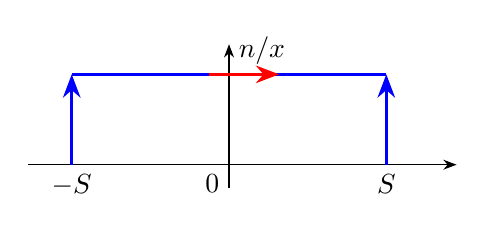
\begin{tikzpicture}[baseline=(current bounding box.center),scale=0.85,>=Stealth]
		\draw[->] (-3.0,0) -- (3.4,0);
		\draw[->] (0,-0.35) -- (0,1.8);
		\node[below] at (-2.35,0) {$-S$};
		\node[below] at (2.35,0) {$S$};
		\node[below left] at (0,0) {$0$};
		\node[above right] at (0,1.35) {$n/x$};
		\draw[blue,very thick,->] (-2.35,0) -- (-2.35,1.35);
		\draw[blue,very thick,->] (2.35,0) -- (2.35,1.35);
		\draw[blue,very thick] (-2.35,1.35) -- (2.35,1.35);
		\draw[red,very thick,->] (-0.3,1.35) -- (0.75,1.35);
	\end{tikzpicture}
	\]
	在两个竖直边上的积分满足估计
	\[
		i\int_0^{n/x}e^{-\pi x(-S+i\eta)^2}\,d\eta
		+
		i\int_{n/x}^{0}e^{-\pi x(S+i\eta)^2}\,d\eta
		\ll
		\frac{n}{x}e^{-\pi xS^2+\pi n^2/x}
		\longrightarrow0
		\qquad (S\to\infty).
	\]
	于是令 $S\to\infty$，得到
	\[
		\int_{\mathbb R+in/x}e^{-\pi xz^2}\,dz
		=
		\int_{\mathbb R}e^{-\pi x\xi^2}\,d\xi
		=
		\frac{1}{\sqrt{x}}.
	\]
	因此
	\[
		\widehat f(n)=\frac{1}{\sqrt{x}}e^{-\pi n^2/x}.
	\]
	代入 Poisson 求和公式，即得
	\[
		\theta(x)=\frac{1}{\sqrt{x}}\theta\left(\frac1x\right).
	\]
\end{proof}

\weekmarker{第 12 周}

\begin{proof}[Theorem 8.1 的证明]
	先设 $\Re(s)>1$。由 Gamma 函数的积分公式，
	\[
	\begin{aligned}
		\pi^{-s/2}\Gamma\left(\frac{s}{2}\right)\zeta(s)
		&=
		\int_0^\infty
		\sum_{n=1}^{\infty}e^{-\pi n^2\xi}
		\xi^{s/2}\frac{d\xi}{\xi} \\
		&=
		\int_0^\infty
		\frac{\theta(\xi)-1}{2}
		\xi^{s/2}\frac{d\xi}{\xi}.
	\end{aligned}
	\]
	这里可以交换求和与积分的次序，因为当 $\xi>0$ 时 $\theta(\xi)$ 绝对收敛。
	注意右端积分只有在 $\Re(s)>1$ 时收敛。事实上，当 $\xi$ 很小时，比如
	$0<\xi<1$，有
	\[
		\theta(\xi)-1\ll \xi^{-1/2},
	\]
	而
	\[
		\int_0^1 \xi^{-1/2}\xi^{s/2}\frac{d\xi}{\xi}
	\]
	只在 $\Re(s)>1$ 时收敛。

	现在把积分拆成两段：
	\[
	\begin{aligned}
		\int_0^\infty
		\frac{\theta(\xi)-1}{2}
		\xi^{s/2}\frac{d\xi}{\xi}
		&=
		\int_0^1
		\frac{\theta(\xi)-1}{2}
		\xi^{s/2}\frac{d\xi}{\xi}
		+
		\int_1^\infty
		\frac{\theta(\xi)-1}{2}
		\xi^{s/2}\frac{d\xi}{\xi}.
	\end{aligned}
	\]
	由 Lemma 8.3，第一项可以写成
	\[
	\begin{aligned}
		\int_0^1
		\frac{\theta(\xi)-1}{2}
		\xi^{s/2}\frac{d\xi}{\xi}
		&=
		\frac12
		\int_0^1
		\left(\xi^{-1/2}\theta\left(\frac1\xi\right)-1\right)
		\xi^{s/2}\frac{d\xi}{\xi} \\
		&=
		\frac12
		\int_0^1
		\xi^{-1/2}
		\left(\theta\left(\frac1\xi\right)-1\right)
		\xi^{s/2}\frac{d\xi}{\xi} \\
		&\qquad
		+
		\frac12
		\int_0^1
		(\xi^{-1/2}-1)\xi^{s/2}\frac{d\xi}{\xi}.
	\end{aligned}
	\]
	在第一项中作变量代换 $u=1/\xi$，得到
	\[
		\frac12
		\int_0^1
		\xi^{-1/2}
		\left(\theta\left(\frac1\xi\right)-1\right)
		\xi^{s/2}\frac{d\xi}{\xi}
		=
		\frac12
		\int_1^\infty
		(\theta(u)-1)u^{(1-s)/2}\frac{du}{u}.
	\]
	另一方面，
	\[
		\frac12
		\int_0^1
		(\xi^{-1/2}-1)\xi^{s/2}\frac{d\xi}{\xi}
		=
		\frac{1}{s-1}-\frac1s
		=
		-\frac1s-\frac{1}{1-s}.
	\]
	总之得到
	\begin{equation}
	\begin{aligned}
		\pi^{-s/2}\Gamma\left(\frac{s}{2}\right)\zeta(s)
		&=
		-\frac1s-\frac{1}{1-s} \\
		&\qquad
		+
		\int_1^\infty
		\frac{\theta(\xi)-1}{2}
		\left(\xi^{s/2}+\xi^{(1-s)/2}\right)
		\frac{d\xi}{\xi}.
	\end{aligned}
	\tag{8.2}
	\end{equation}
	这里注意，右端的积分对所有 $s\in\mathbb C$ 都收敛。因此右端定义了一个亚纯函数，从而给出了 $\zeta(s)$ 到整个复平面的亚纯延拓。并且，式 (8.2) 在把 $s$ 替换成 $1-s$ 时保持不变，于是得到函数方程
	\[
		\pi^{-s/2}\Gamma\left(\frac{s}{2}\right)\zeta(s)
		=
		\pi^{-(1-s)/2}
		\Gamma\left(\frac{1-s}{2}\right)\zeta(1-s).
	\]
	至于 $\zeta(s)$ 的极点，我们已经看出它在半平面 $\Re(s)>0$ 中的唯一极点是 $s=1$，而且这是一个单极点。再由函数方程以及 $\Gamma(s)$ 在 $s=0$ 有一个单极点这个事实，可以看出 $\zeta(s)$ 在 $\mathbb C$ 中除 $s=1$ 以外没有其他极点。
\end{proof}

\begin{remark}
	由 Gamma 函数的性质，函数方程也可以写成
	\[
		\zeta(1-s)=\chi(s)\zeta(s),
		\qquad
		\chi(s)=2(2\pi)^{-s}\Gamma(s)\cos\frac{\pi s}{2},
	\]
	或者等价地写成
	\[
		\zeta(s)
		=
		2^s\pi^{s-1}\sin\frac{\pi s}{2}\Gamma(1-s)\zeta(1-s).
	\]
	由于 $\Gamma(s)$ 与 $\zeta(s)$ 在 $\Re(s)>1$ 时都不为零，上面的恒等式说明 $\zeta(s)$ 在 $\Re(s)<0$ 中的零点恰好是
	\[
		s=-2,-4,-6,\ldots,
	\]
	这些称为平凡零点（trivial zeros）。所有其他零点都位于带状区域
	\[
		0\leq \Re(s)\leq 1,
	\]
	这个区域称为临界带（critical strip）。
\end{remark}

\section{一阶整函数}

本节的目标是把 $\zeta$-函数表达成由它的零点指标化的无穷乘积，这称为 Hadamard 分解（Hadamard factorization）。由于这种分解对一类更一般的全纯函数有效，我们先为一般全纯函数建立定理，然后再应用到特殊情形 $\zeta^*(s)$。

\subsection{复分析中的一个定理}

复分析中一个熟知的定理说，所有满足
\[
	f(s)\ll |s|^\alpha
\]
的整函数（entire function）其实都是多项式，而且次数至多为 $\alpha$。下面的引理给出我们需要的形式。

\begin{lemma}[原文 Lemma 9.1]
	设 $C,\alpha>0$ 为实常数。如果 $g$ 是一个整函数，并且对所有 $s\in\mathbb C$ 满足
	\begin{equation}
		\Re g(s)\leq C(1+|s|^\alpha),
		\tag{9.1}
	\end{equation}
	那么 $g$ 是次数至多为 $\alpha$ 的多项式。
\end{lemma}

\begin{proof}
	不妨假设 $g$ 在 $s=0$ 消失，否则把 $g(s)$ 换成 $g(s)-g(0)$。把 $g$ 写成 Taylor 级数
	\[
		g(s)=\sum_{n=1}^{\infty}(a_n+ib_n)s^n,
	\]
	其中 $a_n,b_n\in\mathbb R$。这个级数在整个复平面上收敛。使用极坐标
	$s=re^{2\pi i\theta}$，则实部有展开
	\[
		\Re g(re^{2\pi i\theta})
		=
		\sum_{n=1}^{\infty}a_n\cos(2\pi n\theta)r^n
		-
		\sum_{n=1}^{\infty}b_n\sin(2\pi n\theta)r^n.
	\]
	回忆正交关系
	\[
		\int_0^1
		\cos(2\pi n\theta)\cos(2\pi \ell\theta)\,d\theta
		=
		\begin{cases}
			\frac12, & n=\ell\neq0,\\
			0, & n\neq \ell,\\
			1, & n=\ell=0,
		\end{cases}
	\]
	以及相应的正弦正交关系。将上式乘以 $\cos(2\pi \ell\theta)$ 并在 $\theta\in[0,1]$ 上积分，可得
	\[
		a_\ell r^\ell
		=
		2\int_0^1
		\Re g(re^{2\pi i\theta})\cos(2\pi\ell\theta)\,d\theta.
	\]
	这里还用到 $g(0)=0$ 以及实部的平均值性质：
	\[
		\int_0^1 \Re g(re^{2\pi i\theta})\,d\theta=\Re g(0)=0.
	\]
	因此由上界 (9.1)，
	\[
		\int_0^1 |\Re g(re^{2\pi i\theta})|\,d\theta
		=
		2\int_0^1 \max\{0,\Re g(re^{2\pi i\theta})\}\,d\theta
		\ll
		1+r^\alpha.
	\]
	于是
	\[
	\begin{aligned}
		|a_\ell|
		&\leq
		\frac{2}{r^\ell}
		\int_0^1 |\Re g(re^{2\pi i\theta})|\,d\theta
		\ll
		r^{\alpha-\ell}.
	\end{aligned}
	\]
	令 $r\to\infty$，当 $\ell>\alpha$ 时得到 $a_\ell=0$。同样地，乘以 $\sin(2\pi\ell\theta)$ 并积分，可以得到 $b_\ell=0$。因此当 $\ell>\alpha$ 时所有系数都为零，故 $g$ 是次数至多为 $\alpha$ 的多项式。
\end{proof}

\begin{definition}[有限阶函数]
	设 $f:\mathbb C\to\mathbb C$ 为整函数。如果存在常数 $\alpha>0$，使得对所有 $s\in\mathbb C$ 都有
	\[
		f(s)=O\left(\exp(|s|^\alpha)\right),
	\]
	则称 $f$ 是有限阶（finite order）的。
\end{definition}

\begin{definition}[阶]
	如果整函数 $f$ 是有限阶的，则数
	\[
		\inf\left\{
		\alpha>0:
		f(s)\ll \exp(|s|^\alpha)
		\right\}
	\]
	称为 $f$ 的阶（order）。
\end{definition}

如果一个有限阶函数在 $\mathbb C$ 上没有零点，那么它有非常特殊的形式。

\begin{lemma}[原文 Lemma 9.2]
	设 $f$ 是有限阶整函数，并且在 $\mathbb C$ 上处处不为零。那么
	\[
		f(s)=\exp(g(s)),
	\]
	其中 $g$ 是一个多项式。更精确地，$g$ 的次数至多为 $f$ 的阶。
\end{lemma}

\begin{proof}
	因为 $f$ 在 $\mathbb C$ 上没有零点，所以可以选取一个全纯的 $\log f(s)$。设
	\[
		g(s)=\log f(s).
	\]
	若 $f$ 的阶为 $\alpha$，则对任意 $\varepsilon>0$，
	\[
		\Re g(s)=\log |f(s)|\ll |s|^{\alpha+\varepsilon}.
	\]
	由 Lemma 9.1 的证明同样可以推出 $g$ 是多项式；令 $\varepsilon\to0$，可知 $g$ 的次数至多为 $\alpha$。
\end{proof}

现在我们需要研究带有零点的有限阶函数。下面的定理给出阶与零点分布之间的关系。

\begin{theorem}[Jensen 公式；原文 Theorem 9.3]
	设 $R>0$。设 $f$ 在圆盘
	\[
		|s|\leq R
	\]
	的某个邻域中全纯，并且 $f$ 在 $s=0$ 处不为零，在圆周 $|s|=R$ 上也不为零。那么
	\[
		\frac{1}{2\pi}
		\int_0^{2\pi}\log |f(Re^{i\theta})|\,d\theta
		=
		\log |f(0)|
		+
		\sum_\rho \log\frac{R}{|\rho|},
	\]
	其中 $\rho$ 遍历 $f$ 在 $|\rho|<R$ 中的零点，并按重数计算。
\end{theorem}

\begin{proof}
	把 $f$ 分解为
	\[
		f(s)=\widetilde f(s)\prod_\rho (s-\rho),
	\]
	其中 $\rho$ 遍历圆盘 $|s|<R$ 中的零点，并按重数计算；而 $\widetilde f$ 在 $|s|\leq R$ 上全纯且不为零。于是
	\[
		\log |f(s)|
		=
		\log|\widetilde f(s)|
		+
		\sum_\rho \log|s-\rho|.
	\]
	因此只需处理下面两种情形。

	第一，如果 $f$ 在 $|s|\leq R$ 中没有零点，那么 $\log f(s)$ 是全纯函数。由 Cauchy 公式，
	\[
		\log |f(0)|
		=
		\Re \log f(0)
		=
		\frac{1}{2\pi}\int_0^{2\pi}
		\Re \log f(Re^{i\theta})\,d\theta
		=
		\frac{1}{2\pi}\int_0^{2\pi}
		\log |f(Re^{i\theta})|\,d\theta.
	\]

	第二，考虑 $f(s)=s-\xi$，其中 $|\xi|<R$。写
	\[
		f(s)=f_1(s)f_2(s),
		\qquad
		f_1(s)=\frac{s-\xi}{R^2-\overline{\xi}s},
		\qquad
		f_2(s)=R^2-\overline{\xi}s.
	\]
	当 $|s|=R$ 时，
	\[
		|f_1(s)|=\frac1R.
	\]
	另一方面，$f_2$ 在圆盘中没有零点，所以由第一种情形，
	\[
		\frac{1}{2\pi}\int_0^{2\pi}
		\log |f_2(Re^{i\theta})|\,d\theta
		=
		\log |f_2(0)|
		=
		\log R^2.
	\]
	合并起来得到
	\[
		\frac{1}{2\pi}\int_0^{2\pi}
		\log |Re^{i\theta}-\xi|\,d\theta
		=
		-\log R+\log R^2
		=
		\log R.
	\]
	把这两个情形代回上面的分解，即得 Jensen 公式。
\end{proof}

作为 Jensen 公式的推论，我们有下面的零点计数估计。

\begin{theorem}[原文 Theorem 9.4]
	设 $\alpha>0$，并设 $f$ 是阶为 $\alpha$ 的整函数。那么对所有 $R\geq1$ 以及任意 $\varepsilon>0$，有
	\[
		\sum_{|\rho|\leq R}1
		\ll
		R^{\alpha+\varepsilon},
	\]
	其中 $\rho$ 遍历 $f$ 在 $|z|<R$ 中的零点，并按重数计算。
\end{theorem}

\begin{proof}
	不妨假设 $f(0)\neq0$；如果不是这样，则把 $f(s)$ 换成 $f(s)s^{-m}$，其中 $m$ 是合适的整数。也可以假设 $f$ 在圆周 $|s|=3R$ 上没有零点；否则把 $R$ 换成 $R+\delta$，其中某个实数 $\delta\in(0,1)$ 可以避开零点。

	由 Theorem 9.3，并使用 $f$ 的阶为 $\alpha$，得到
	\[
	\begin{aligned}
		\sum_{|\rho|\leq R}1
		&\leq
		\sum_{|\rho|\leq R}\log\frac{3R}{|\rho|} \\
		&\leq
		\sum_{|\rho|\leq 3R}\log\frac{3R}{|\rho|} \\
		&=
		-\log|f(0)|
		+
		\frac{1}{2\pi}
		\int_0^{2\pi}
		\log|f(3Re^{i\theta})|\,d\theta
		\ll R^{\alpha+\varepsilon}.
	\end{aligned}
	\]
	这就证明了定理。
\end{proof}

\begin{remark}
	作为这个定理的一个推论，如果 $f$ 的阶为 $\alpha$，那么对任何 $\varepsilon>0$，
	\[
		\sum_\rho \frac{1}{|\rho|^{\alpha+\varepsilon}}<\infty,
	\]
	其中 $\rho$ 遍历 $f$ 的所有非零零点，并按重数计算。证明作为练习。
\end{remark}

现在我们准备证明本节的主要定理。

\begin{theorem}[Hadamard 分解；原文 Theorem 9.5]
	设 $f$ 是阶至多为 $1$ 的整函数。设 $k\geq0$ 为 $f$ 在 $s=0$ 处零点的阶数。那么存在常数 $A,B\in\mathbb C$，使得
	\[
		f(s)
		=
		e^{A+Bs}s^k
		\prod_\rho
		\left(1-\frac{s}{\rho}\right)e^{s/\rho},
	\]
	其中 $\rho$ 遍历 $f$ 的所有非零零点，并按重数计算；乘积在不含零点的有界区域上一致收敛。
\end{theorem}

\begin{proof}
	先说明乘积的收敛性。设 $K\subset\mathbb C$ 为紧集。$K$ 中的零点只有有限多个。对于 $s\in K$，并且对 $K$ 外的零点 $\rho$，有
	\[
		\left(1-\frac{s}{\rho}\right)e^{s/\rho}
		=
		1+O_K\left(\frac{1}{|\rho|^2}\right).
	\]
	回忆：如果 $\sum a_n$ 绝对收敛，那么 $\prod(1+a_n)$ 收敛。由于 $f$ 的阶至多为 $1$，Theorem 9.4 推出
	\[
		\sum_\rho\frac1{|\rho|^2}<\infty.
	\]
	于是乘积
	\[
		P(s):=
		\prod_\rho
		\left(1-\frac{s}{\rho}\right)e^{s/\rho}
	\]
	在有界区域上一致收敛，并定义一个整函数。并且 $P$ 的零点恰好就是 $f$ 的非零零点，重数也相同。

	因此，在先把 $s=0$ 处的零点因子 $s^k$ 分离出来以后，商
	\[
		\frac{f(s)}{s^kP(s)}
	\]
	是一个整函数，并且在 $\mathbb C$ 上处处不为零。下面证明这个商的阶至多为 $1$。由 Lemma 9.2，这将给出定理。

	因为 $f$ 本身按假设是阶至多为 $1$ 的，我们已经有 $f(s)$ 的上界。因此只需要给出 $P(s)$ 的下界。由于
	\[
		\sum_\rho\frac1{|\rho|^2}<\infty,
	\]
	所有区间
	\[
		\left(|\rho|-\frac1{|\rho|^2},\,|\rho|+\frac1{|\rho|^2}\right)
	\]
	的总长度是有限的。因此存在任意大的实数 $R$，使得
	\begin{equation}
		\bigl|R-|\rho|\bigr|>\frac1{|\rho|^2}
		\qquad
		\text{对所有零点 }\rho.
	\tag{9.2}
	\end{equation}
	下面估计 $P(s)$ 在圆周 $|s|=R$ 上的大小。写
	\[
		P(s)=P_1(s)P_2(s)P_3(s),
	\]
	其中
	\[
		P_1(s)=
		\prod_{|\rho|\leq R/2}
		\left(1-\frac{s}{\rho}\right)e^{s/\rho},
	\]
	\[
		P_2(s)=
		\prod_{R/2<|\rho|\leq 2R}
		\left(1-\frac{s}{\rho}\right)e^{s/\rho},
	\]
	以及
	\[
		P_3(s)=
		\prod_{|\rho|>2R}
		\left(1-\frac{s}{\rho}\right)e^{s/\rho}.
	\]

	先估计 $P_1(s)$。对于满足 $|\rho|\leq R/2$ 的零点 $\rho$，有
	\[
		\left|
		\left(1-\frac{s}{\rho}\right)e^{s/\rho}
		\right|
		\geq
		\left(\frac{|s|}{|\rho|}-1\right)e^{-|s|/|\rho|}
		>
		\exp\left(-\frac{R}{|\rho|}\right),
	\]
	当 $R$ 充分大时成立。因此
	\[
		|P_1(s)|
		>
		\exp\left(
		-\sum_{|\rho|\leq R/2}\frac{R}{|\rho|}
		\right).
	\]
	又因为
	\[
		\sum_{|\rho|\leq R/2}\frac1{|\rho|}
		\leq
		\left(\frac{R}{2}\right)^\varepsilon
		\sum_\rho \frac1{|\rho|^{1+\varepsilon}},
	\]
	所以
	\[
		|P_1(s)|>\exp(-R^{1+\varepsilon}).
	\]

	再估计 $P_2(s)$。对于满足 $R/2<|\rho|\leq2R$ 的零点，由 (9.2) 可得
	\[
	\begin{aligned}
		\left|
		\left(1-\frac{s}{\rho}\right)e^{s/\rho}
		\right|
		&\geq
		e^{-2}\left|1-\frac{s}{\rho}\right| \\
		&\geq
		e^{-2}\frac{\bigl||s|-|\rho|\bigr|}{|\rho|}
		\geq
		e^{-2}\frac{\bigl|R-|\rho|\bigr|}{2R}
		\geq
		\frac{c}{R^3}
	\end{aligned}
	\]
	其中 $c>0$ 为某个常数。由 Theorem 9.4，在区域 $R/2<|\rho|\leq2R$ 中至多有 $O(R^{1+\varepsilon})$ 个零点。因此
	\[
		|P_2(s)|
		\geq
		(cR^{-3})^{CR^{1+\varepsilon}}
		>
		\exp(-R^{1+2\varepsilon})
	\]
	当 $R$ 充分大时成立。

	最后估计 $P_3(s)$。如果 $|\rho|>2R$，则 $|s/\rho|<1/2$。利用不等式
	\[
		\left|\left(1-\frac{s}{\rho}\right)e^{s/\rho}\right|
		>
		\exp\left(-c\left|\frac{s}{\rho}\right|^2\right),
		\qquad |s/\rho|<\frac12,
	\]
	其中 $c$ 取充分小的常数，于是
	\[
		|P_3(s)|
		>
		\exp\left(
		-cR^2\sum_{|\rho|>2R}\frac1{|\rho|^2}
		\right).
	\]
	注意到
	\[
		\sum_{|\rho|>2R}\frac1{|\rho|^2}
		\leq
		(2R)^{-1+\varepsilon}
		\sum_\rho\frac1{|\rho|^{1+\varepsilon}},
	\]
	所以
	\[
		|P_3(s)|
		>
		\exp(-R^{1+2\varepsilon})
	\]
	当 $R$ 充分大时成立。

	把 $P_1,P_2,P_3$ 的下界相乘，得到
	\[
		|P(s)|>\exp(-3R^{1+2\varepsilon})
		>
		\exp(-R^{1+3\varepsilon})
		\qquad (|s|=R),
	\]
	其中 $R$ 充分大并满足 (9.2)。另一方面，由于 $f$ 的阶至多为 $1$，有
	\[
		f(s)\ll \exp(R^{1+\varepsilon})
		\qquad (|s|=R).
	\]
	于是
	\begin{equation}
		\frac{f(s)}{s^kP(s)}
		\ll
		\exp(R^{1+4\varepsilon})
		\qquad (|s|=R).
	\tag{9.3}
	\end{equation}
	最后，由于 $\sum_\rho 1/|\rho|^2$ 收敛，可以选取一列实数 $\{R_j\}_{j=1}^{\infty}$，使得
	\[
		\lim_{j\to\infty}R_j=\infty,
		\qquad
		|R_{j+1}-R_j|\leq1,
	\]
	并且每个 $R_j$ 都满足 (9.2)。把 (9.3) 用在 $|s|=R_j$ 上，再用最大模原理，得到
	\[
		\frac{f(s)}{s^kP(s)}
		\ll
		\exp\left((|s|+1)^{1+4\varepsilon}\right)
		\ll
		\exp(|s|^{1+5\varepsilon}).
	\]
	这说明 $f/(s^kP)$ 的阶至多为 $1$。由 Lemma 9.2，
	\[
		\frac{f(s)}{s^kP(s)}=e^{A+Bs}
	\]
	对某些常数 $A,B\in\mathbb C$ 成立。代回 $P(s)$ 的定义，即得所需分解。
\end{proof}

\begin{remark}
	如果 $f$ 是阶为 $1$ 的整函数，那么
	\[
		\sum_\rho \frac1{|\rho|}
	\]
	可能收敛，也可能不收敛。在收敛的情形中，可以得到没有 $1+\varepsilon$ 出现在指数里的估计，即
	\[
		f(s)\ll e^{c|s|}
	\]
	对某个常数 $c>0$ 成立。
\end{remark}

\begin{proof}
	由 Hadamard 分解，
	\[
		f(s)=s^k e^{A+Bs}
		\prod_\rho
		\left(1-\frac{s}{\rho}\right)e^{s/\rho}.
	\]
	若 $\sum_\rho 1/|\rho|<\infty$，则
	\[
	\begin{aligned}
		|f(s)|
		&\ll
		|s|^k e^{|B||s|}
		\prod_\rho
		\left(1+\frac{|s|}{|\rho|}\right)e^{|s|/|\rho|} \\
		&\ll
		e^{|s|}e^{|B||s|}
		\prod_\rho e^{2|s|/|\rho|}
		\ll
		e^{c|s|},
	\end{aligned}
	\]
	其中
	\[
		c=1+|B|+2\sum_\rho\frac1{|\rho|}
	\]
	是某个常数。
\end{proof}

\weekmarker{第 13 周}

下面记录两个 Hadamard 分解的例子。

\begin{example}[Hadamard 分解的例子]
	\[
		\frac{1}{\Gamma(s)}
		=
		se^{\gamma s}
		\prod_{\ell=1}^{\infty}
		\left(1+\frac{s}{\ell}\right)e^{-s/\ell}.
	\]
	另外，
	\[
		\sin \pi s
		=
		se^{A+Bs}
		\prod_{n=1}^{\infty}\left(1-\frac{s^2}{n^2}\right).
	\]
	回忆我们曾经用这个公式推出
	\[
		\frac{\sin \pi s}{\pi s}
		=
		\prod_{n\geq 1}\left(1-\frac{s^2}{n^2}\right),
	\]
	从而证明反射公式
	\[
		\Gamma(s)\Gamma(1-s)=\frac{\pi}{\sin \pi s}.
	\]
\end{example}

\subsection{\texorpdfstring{\(\zeta^*(s)\) 的 Hadamard 分解}{zeta*(s) 的 Hadamard 分解}}

现在把 Hadamard 分解，即 Theorem 9.5，应用到
$f(s)=\zeta^*(s)$，也就是整化的 Riemann $\zeta$-函数。

\begin{theorem}[原文 Theorem 9.6；\texorpdfstring{\(\zeta^*(s)\)}{zeta*(s)} 的 Hadamard 分解]
	$\zeta^*(s)$ 是一个阶为 $1$ 的整函数，并且满足
	\[
		\zeta^*(s)
			=
			e^{Bs}\prod_\rho
			\left(1-\frac{s}{\rho}\right)e^{s/\rho},
		\]
		其中 $B$ 是一个复常数，乘积遍历 $\zeta^*(s)$ 的零点；也就是说，
		$\rho$ 遍历 $\zeta(s)$ 的非平凡零点，并按重数计算。
\end{theorem}

\begin{proof}
	由于 $\zeta^*(s)$ 已经是整函数，为了应用 Theorem 9.5，我们只需要验证它的阶为 $1$。
	借助函数方程
	\[
		\zeta^*(s)=\zeta^*(1-s),
	\]
	只需在半平面 $\Re(s)\geq 1/2$ 中估计 $\zeta^*(s)$。
	由 Stirling 公式，
	\[
		\log\Gamma(s)
		=
		\left(s-\frac12\right)\log s-s+\frac{\log 2\pi}{2}
		+O_\delta\left(\frac1{|s|}\right),
	\]
	从而
	\[
		\log|\Gamma(s)|
		=
		\Re\log\Gamma(s)
		\leq |s|\log |s|.
	\]
	特别地，
	\[
		\Gamma\left(\frac{s}{2}\right)\ll e^{|s|\log |s|}.
	\]
	另一方面，对 $\zeta(s)$，由前面得到的表达式
	\[
		\zeta(s)
		=
		\frac{1}{s-1}
		+1
		-s\int_1^\infty \frac{\rho(\xi)}{\xi^{s+1}}\,d\xi
	\]
	可知
	\[
		\zeta(s)\ll |s|
		\qquad (|s|\to\infty)
	\]
	在这里所需的区域内成立。因此
	\[
		\zeta^*(s)
		=
		s(s-1)\pi^{-s/2}\Gamma\left(\frac{s}{2}\right)\zeta(s)
		\ll
		e^{2|s|\log |s|}.
	\]
	这说明 $\zeta^*(s)$ 的阶至多为 $1$。

	反过来，令 $s\to\infty$ 沿实数趋于无穷。由
	\[
		\Gamma(s)\sim e^{s\log s}
	\]
	可得，对实数 $s$，
	\[
		\zeta^*(s)\gg e^{|s/2|\log |s/2|}.
	\]
	所以 $\zeta^*(s)$ 的阶至少为 $1$。于是 $\zeta^*(s)$ 的阶恰好为 $1$。

	由 Hadamard 分解（Theorem 9.5），
	\[
		\zeta^*(s)
		=
		e^{A+Bs}\prod_\rho
		\left(1-\frac{s}{\rho}\right)e^{s/\rho}.
	\]
	这里 $A=0$，因为
	\[
		\zeta^*(0)=\zeta^*(1)
		=
		\lim_{s\to1}(s-1)\zeta(s)
		=
		1.
	\]
	因此得到所需公式。
\end{proof}

\begin{remark}
	$\zeta^*(s)$ 的零点恰好就是 $\zeta(s)$ 的非平凡零点（non-trivial zeros）。
	因此，下文在 $\zeta^*(s)$ 或 $\zeta(s)$ 的零点公式中出现的 $\sum_\rho$ 或 $\prod_\rho$，
	除非另有说明，都表示 $\rho$ 遍历这些非平凡零点，并按重数计算；
	若求和号附带 $|\Im\rho|<T$ 等条件，则是在这些非平凡零点中再加该条件。
\end{remark}

\begin{remark}
	$\zeta(s)$ 的零点关于直线 $\Re(s)=1/2$ 和直线 $\Im(s)=0$ 对称。
	事实上，若 $\zeta(\rho)=0$，则
	\[
		\zeta(\overline{\rho})
		=
		\overline{\zeta(\rho)}
		=
		0,
	\]
	而由函数方程可得相应的关于 $\Re(s)=1/2$ 的对称性。
\end{remark}

\begin{theorem}[原文 Theorem 9.7]
	$\zeta(s)$ 的非平凡零点集是无限的。更精确地说，
	\[
		\sum_\rho \frac{1}{|\rho|^\sigma}
	\]
	在 $\sigma=1$ 时发散，而对所有 $\sigma>1$ 收敛。
\end{theorem}

\begin{proof}
	当 $\sigma=1+\varepsilon$ 时，收敛性由 $\zeta^*(s)$ 是阶为 $1$ 的整函数以及 Theorem 9.4 得到。
	而
	\[
		\sum_\rho \frac1{|\rho|}
	\]
	的发散性则来自 Theorem 9.5 后面的备注。既然这个级数发散，$\zeta(s)$ 的非平凡零点必然有无穷多个。
\end{proof}

Theorem 9.7 还有下面的推论。由于若 $\rho$ 是 $\zeta(s)$ 的非平凡零点，则
$\overline{\rho}$ 也是 $\zeta(s)$ 的非平凡零点，并且
\[
	0\leq
	\frac1{\rho}+\frac1{\overline{\rho}}
	=
	\frac{2\Re(\rho)}{|\rho|^2}
	\leq
	\frac{2}{|\rho|^2},
\]
所以
\[
	\lim_{x\to\infty}\sum_{|\rho|\leq x}\frac1{\rho}
	=
	\sum_{\Im\rho>0}\left(\frac1{\rho}+\frac1{\overline{\rho}}\right)
\]
是收敛的。因此
\[
	\sum_\rho \frac1{\rho}<\infty.
\]
这里记号 $\sum_\rho 1/\rho$ 指的是在 $\zeta(s)$ 的非平凡零点上按 $|\rho|$ 截断的极限
\[
	\lim_{x\to\infty}\sum_{|\rho|\leq x}\frac1{\rho}.
\]
但是要记住，这个和并不是绝对收敛的；如果改变求和顺序，值可能发生变化。

稍后我们会推出整化 $\zeta$-函数的对数导数关于零点的表达式。为此先证明下面的引理。

\begin{lemma}[原文 Lemma 9.8]
	存在 $K>0$，使得
	\[
		\zeta(s)\ll |s|^K
	\]
	对区域 $\sigma\geq -5$ 且 $|t|\geq 1$ 中的所有 $s=\sigma+it$ 成立。
	例如 $K=5$ 可以取。
\end{lemma}

\begin{proof}
	当 $\sigma>1+\varepsilon$ 时，
	\[
		\zeta(s)\ll 1.
	\]
	前面已经看到，在相应的右半平面中，
	\[
		\zeta(s)\ll |s|.
	\]
	最后，对区域 $-5\leq \sigma\leq 1/2$，使用 $\zeta(s)$ 的函数方程以及 Stirling 公式
	\[
		\Gamma(\sigma+it)
		=
		\sqrt{2\pi}|t|^{\sigma-1/2}e^{-\frac{\pi}{2}|t|}
		\left(1+O\left(\frac1{|t|}\right)\right),
	\]
	即可得到
	\[
		\zeta(s)\ll |s|^K
	\]
	对某个 $K>0$ 成立。
\end{proof}

记
\[
	N(T)
	:=
	\sum_{\substack{\rho\\ |\Im\rho|\leq T}}1,
\]
其中 $\rho$ 遍历 $\zeta(s)$ 的非平凡零点；也就是说，$N(T)$ 是
$\zeta(s)$ 的虚部绝对值不超过 $T$ 的非平凡零点个数。

\begin{lemma}[原文 Lemma 9.9]
	对所有 $T\geq 2$，有
	\[
		N(T)-N(T-1)\ll \log T,
		\qquad
		N(T)\ll T\log T.
	\]
\end{lemma}

\begin{proof}
	令
	\[
		\tau=2+iT,
	\]
	并选取 $r\in[3,4]$，使得
	\[
		\zeta^*\left(\tau+re^{2\pi i\theta}\right)\neq 0
		\qquad
		(\theta\in\mathbb R).
	\]
	把 Jensen 公式（Theorem 9.3）应用到函数
	\[
		f(s)=\zeta^*(\tau+s),
	\]
	得到
	\[
		\sum_{\rho,\ |\rho-\tau|\leq r}
		\log\frac{r}{|\rho-\tau|}
		=
			\frac1{2\pi}
				\int_0^{2\pi}
				\log|\zeta^*(\tau+re^{i\theta})|\,d\theta
				-\log|\zeta^*(\tau)|.
	\]
		这里的 $\rho$ 是 $\zeta^*(s)$ 的零点，也就是 $\zeta(s)$ 的非平凡零点。
		由 Lemma 9.8，右端满足
	\[
		\ll \log T.
	\]
	对左端，每一项
	\[
		\log\frac{r}{|\rho-\tau|}
	\]
		都是非负的。限制在满足 $\Im\rho\in[T-1,T]$ 的非平凡零点上，由于非平凡零点满足
	$0\leq\Re\rho\leq 1$，且 $\tau=2+iT$，这些零点都落在以 $\tau$ 为圆心、半径 $r$ 的圆盘中所需的矩形范围内：
	\[
	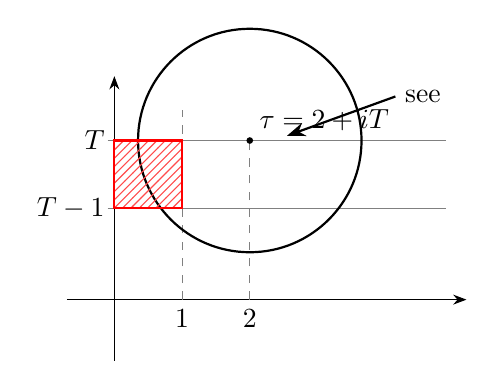
\begin{tikzpicture}[baseline=(current bounding box.center),scale=0.86,>=Stealth]
		\draw[->] (-0.7,0) -- (5.2,0);
		\draw[->] (0,-0.9) -- (0,3.3);
		\node[left] at (0,2.35) {$T$};
		\node[left] at (0,1.35) {$T-1$};
		\draw[gray] (-0.1,2.35) -- (4.9,2.35);
		\draw[gray] (-0.1,1.35) -- (4.9,1.35);
		\draw[gray,dashed] (1,0) -- (1,2.8);
		\draw[gray,dashed] (2,0) -- (2,2.35);
		\node[below] at (1,0) {$1$};
		\node[below] at (2,0) {$2$};
		\coordinate (tau) at (2,2.35);
		\fill (tau) circle (1.4pt);
		\node[above right] at (tau) {$\tau=2+iT$};
		\draw[thick] (tau) circle (1.65);
		\draw[red,pattern=north east lines,pattern color=red!70] (0,1.35) rectangle (1,2.35);
		\draw[red,thick] (0,1.35) rectangle (1,2.35);
		\draw[->,thick] (4.15,3.0) -- (2.55,2.42);
		\node[right] at (4.15,3.0) {see};
	\end{tikzpicture}
	\]
	于是
	\[
		\log\frac{3}{\sqrt5}\bigl(N(T)-N(T-1)\bigr)
		\leq
		\sum_{\substack{\rho\\ \Im\rho\in[T-1,T]}}
		\log\frac{r}{|\rho-\tau|}
		\ll
		\log T.
	\]
	所以
	\[
		N(T)-N(T-1)\ll \log T.
	\]
	进一步求和得
	\[
		N(T)\ll T\log T.
	\]
\end{proof}

\chapter{素数定理}
\label{chap:prime-number-theorem}

现在我们有了证明素数定理（prime number theorem）的工具。目标是证明
\[
	\psi(x)
	:=
	\sum_{n\leq x}\Lambda(n)
	=
	x+\text{``error term''}.
\]
由于
\[
	\sum_{n=1}^{\infty}\frac{\Lambda(n)}{n^s}
	=
	-\frac{\zeta'}{\zeta}(s),
\]
想法是使用 Perron 公式（Perron's formula），把 $\psi(x)$ 写成形如
\[
	\frac{1}{2\pi i}
	\int
	-\frac{\zeta'}{\zeta}(s)\frac{x^s}{s}\,ds
\]
的复积分，然后把积分直线移动到 $\Re(s)=1$ 的左边。在这个过程中，$s=1$ 处的留数会给出 $\psi(x)$ 渐近公式中的主项；剩下需要说明的是余下积分相对于主项是低阶项。

\section{\texorpdfstring{\(\zeta'/\zeta(s)\)}{zeta'/zeta(s)} 的性质}

因为与 $\Lambda(n)$ 关联的 Dirichlet 级数是
\[
	\sum_{n=1}^{\infty}\frac{\Lambda(n)}{n^s}
	=
	-\frac{\zeta'}{\zeta}(s),
\]
我们需要理解 $\zeta'/\zeta(s)$ 的性质。

首先考虑半平面 $\Re(s)\geq 2$。有
\[
	\left|\frac{\zeta'}{\zeta}(s)\right|
	\leq
	\sum_{n\geq1}\frac{\Lambda(n)}{n^\sigma}
	=
	-\frac{\zeta'}{\zeta}(\sigma).
\]
由于
\[
	-\frac{\zeta'}{\zeta}(\sigma)
	=
	\frac1{\sigma-1}+O(1),
\]
所以当 $\Re(s)\geq 2$ 时，
\begin{equation}
	\frac{\zeta'}{\zeta}(s)\ll 1.
	\tag{10.1}
\end{equation}

其次考虑区域 $\Re(s)\leq -1$，并假设
\[
	|s+2n|\geq \frac14
	\qquad (n\in\mathbb N).
\]
由函数方程
\[
	\zeta(s)
	=
	2^s\pi^{s-1}\sin\left(\frac{\pi s}{2}\right)\Gamma(1-s)\zeta(1-s),
\]
等价地，
\[
	\zeta(1-s)
	=
	2^{-s}\pi^{-s}\cos\left(\frac{\pi s}{2}\right)\Gamma(s)\zeta(s).
\]
取对数导数，得到
\[
	-\frac{\zeta'}{\zeta}(1-s)
	=
	-\log 2\pi
	-\frac{\pi}{2}\tan\left(\frac{\pi s}{2}\right)
	+\frac{\Gamma'}{\Gamma}(s)
	+\frac{\zeta'}{\zeta}(s).
\]
这里若 $s$ 远离相应的极点，例如满足上面的 $|s+2n|\geq 1/4$，则三角函数项有界。于是当 $\Re(s)\leq -1$ 且
$|s+2n|\geq 1/4$ 对所有 $n\in\mathbb N$ 成立时，
\[
	\frac{\zeta'}{\zeta}(s)\ll \log |s|.
\]

现在剩下要考虑的是带状区域
\[
	-1\leq \Re(s)\leq 2.
\]

\begin{lemma}[原文 Lemma 10.1]
	对所有 $s=\sigma+it\in\mathbb C$，若
	\[
		-1\leq \sigma\leq 2,
		\qquad
		|t|\geq 2,
	\]
	则
	\[
		\frac{\zeta'}{\zeta}(s)
		=
			\sum_{\substack{\rho\\ |\Im\rho-t|<1}}
			\frac1{s-\rho}
			+
			O(\log |t|).
		\]
		其中 $\rho$ 遍历 $\zeta(s)$ 的非平凡零点。
	\end{lemma}

	\begin{proof}
		对
	\[
		\zeta^*(s)
		=
		s(s-1)\pi^{-s/2}\Gamma\left(\frac{s}{2}\right)\zeta(s)
	\]
	以及 Hadamard 分解
	\[
			\zeta^*(s)
			=
			e^{Bs}\prod_\rho
			\left(1-\frac{s}{\rho}\right)e^{s/\rho}
		\]
		其中 $\rho$ 遍历 $\zeta(s)$ 的非平凡零点。
			取对数导数，得到
	\[
		\frac{(\zeta^*)'}{\zeta^*}(s)
		=
		\frac1s+\frac1{s-1}
		-\frac12\log\pi
		+\frac12\frac{\Gamma'}{\Gamma}\left(\frac{s}{2}\right)
		+
		\frac{\zeta'}{\zeta}(s),
	\]
	同时
	\[
		\frac{(\zeta^*)'}{\zeta^*}(s)
		=
		B+
		\sum_\rho
		\left(\frac1{s-\rho}+\frac1{\rho}\right).
	\]
	因此
	\[
		\frac{\zeta'}{\zeta}(s)
		=
		-\frac1s-\frac1{s-1}
		+\frac12\log\pi
		-\frac12\frac{\Gamma'}{\Gamma}\left(\frac{s}{2}\right)
		+
		\sum_\rho
		\left(\frac1{s-\rho}+\frac1{\rho}\right)
		+
		B.
	\]
	顺便记下，由 Gamma 函数的性质还可以进一步推出
	\[
		\frac{\zeta'}{\zeta}(s)
		=
		-\frac1{s-1}
		+
		\sum_\rho
		\left(\frac1{s-\rho}+\frac1{\rho}\right)
		+
		\sum_{m=1}^{\infty}
		\left(\frac1{s+2m}-\frac1{2m}\right)
		+
		\frac{\log\pi}{2}
		+
		B.
	\]
	由 Stirling 公式可知
	\[
		\frac{\Gamma'}{\Gamma}(s)
		=
		\log s+O_\varepsilon\left(\frac1{|s|}\right).
	\]
	所以当 $-1\leq\sigma\leq 2$ 且 $|t|\geq2$ 时，
	\begin{equation}
		\frac{\zeta'}{\zeta}(s)
		=
		\sum_\rho
		\left(\frac1{s-\rho}+\frac1{\rho}\right)
		+
		O(\log |t|).
		\tag{10.2}
	\end{equation}
	把 $s=2+it$ 代入，得到
	\begin{equation}
		\frac{\zeta'}{\zeta}(2+it)
		=
		\sum_\rho
		\left(\frac1{2+it-\rho}+\frac1{\rho}\right)
		+
		O(\log |t|).
		\tag{10.3}
	\end{equation}
	而由 (10.1)，左端是 $O(1)$。用 (10.2) 减去 (10.3)，得到
	\[
		\frac{\zeta'}{\zeta}(s)
		=
		\sum_\rho
		\left(
			\frac1{s-\rho}
			-
			\frac1{2+it-\rho}
		\right)
		+
		O(\log |t|).
	\]

		先看满足 $|\Im\rho-t|\leq1$ 的非平凡零点。由 Lemma 9.9，
	\[
		\sum_{|\Im\rho-t|\leq1}\frac1{|2+it-\rho|}
		\leq
		\sum_{|\Im\rho-t|\leq1}1
		\ll
		\log |t|.
	\]
		接着考虑满足 $|\Im\rho-t|>1$ 的非平凡零点。此时
	\[
		|s-\rho|\asymp |t-\Im\rho|.
	\]
	因此
	\[
		\frac1{s-\rho}
		-
		\frac1{2+it-\rho}
		=
		\frac{2-\sigma}{(s-\rho)(2+it-\rho)}
		\ll
		\frac1{|t-\Im\rho|^2}.
	\]
	于是
	\[
	\begin{aligned}
		&
		\sum_{|\Im\rho-t|>1}
		\left(
			\frac1{s-\rho}
			-
			\frac1{2+it-\rho}
		\right) \\
		&\qquad\ll
		\sum_{n\geq1}
		\sum_{\substack{\rho\\ n\leq |\Im\rho-t|\leq n+1}}
		\frac1{|t-\Im\rho|^2} \\
		&\qquad\ll
		\sum_{n\geq1}\frac{\log(|t|+n)}{n^2}
		\ll
		\sum_{n\geq1}\frac{\log |t|\log n}{n^2}
		\ll
		\log |t|.
	\end{aligned}
	\]
	综上，
	\[
		\frac{\zeta'}{\zeta}(s)
		=
		\sum_{\substack{\rho\\ |\Im\rho-t|<1}}
		\frac1{s-\rho}
		+
		O(\log |t|).
	\]
\end{proof}

\section{显式公式}

回忆
\[
	\psi(x)=\sum_{n\leq x}\Lambda(n).
\]
由于 $\psi(x)$ 在素数幂处有不连续点，我们定义
\[
	\psi_0(x)
	:=
	\begin{cases}
		\psi(x), & x\notin\mathbb Z,\\
		\psi(x)-\dfrac{\Lambda(x)}{2}, & x\in\mathbb Z.
	\end{cases}
\]

\begin{theorem}[显式公式；原文 Theorem 10.2]
	对 $x>2$，有
	\[
		\psi_0(x)
		=
		x
		-
		\sum_\rho \frac{x^\rho}{\rho}
		-
		\frac{\zeta'}{\zeta}(0)
		-
		\frac12\log(1-x^{-2}).
	\]
	其中 $\rho$ 遍历 $\zeta(s)$ 的非平凡零点。
\end{theorem}

这里
\[
	-\frac12\log(1-x^{-2})
	=
	\sum_{m=1}^{\infty}\frac{x^{-2m}}{2m}.
\]
就像 Perron 公式一样，这个公式由下面的定理令 $T\to\infty$ 得到。

\begin{theorem}[有效显式公式；原文 Theorem 10.3]
	对 $x,T>2$，有
	\begin{equation}
		\psi_0(x)
		=
		x
		-
		\sum_{\substack{\rho\\ |\Im\rho|<T}}\frac{x^\rho}{\rho}
		-
		\frac{\zeta'}{\zeta}(0)
		-
		\frac12\log(1-x^{-2})
		+
		R(x,T),
		\tag{10.4}
	\end{equation}
	这里 $\rho$ 遍历 $\zeta(s)$ 的非平凡零点，并且只取满足
	$|\Im\rho|<T$ 的那些零点；其中
	\[
		R(x,T)
		\ll
		\frac{x}{T}(\log xT)^2
		+
		\log x\min\left(1,\frac{x}{T\langle x\rangle}\right),
	\]
	并且
	\[
		\langle x\rangle
		:=
		\min\{|x-p^\ell|:\ p\in\mathbb P,\ \ell\in\mathbb N,\ x\neq p^\ell\}.
	\]
\end{theorem}

\begin{proof}
	回忆 Perron 公式说：若
	\[
		L_f(s)=\sum_{n=1}^{\infty}\frac{f(n)}{n^s}
	\]
	在 $s=c$ 处绝对收敛，则
	\[
		\sum_{n\leq x}^{*}f(n)
		=
		\frac1{2\pi i}
		\int_{c-iT}^{c+iT}
		L_f(s)\frac{x^s}{s}\,ds
		+
		O\left(
		\sum_{n=1}^{\infty}
		\frac{x^c|f(n)|}{n^c(1+T|\log(x/n)|)}
		+
		\frac{c}{T}|f(x)|
		\right).
	\]
	这里星号表示：如果 $x\in\mathbb Z$，那么最后一项 $f(x)$ 要替换成 $f(x)/2$。

	把公式应用到 $f(n)=\Lambda(n)$，并取
	\[
		c=1+\frac1{\log x},
	\]
	得到
	\[
		\psi_0(x)
		=
		\frac1{2\pi i}
		\int_{c-iT}^{c+iT}
		-\frac{\zeta'}{\zeta}(s)\frac{x^s}{s}\,ds
		+
		O(\Sigma),
	\]
	其中
	\[
		\Sigma
		=
		\sum_{\substack{n=1\\ n\neq x}}^{\infty}
		\frac{x^c\Lambda(n)}{n^c(1+T|\log(x/n)|)}
		+
		\frac{c}{T}\Lambda(x).
	\]
	我们需要证明
	\begin{equation}
		\Sigma
		\ll
		\frac{x(\log x)^2}{T}
		+
		\log x\min\left(1,\frac{x}{T\langle x\rangle}\right).
		\tag{10.5}
	\end{equation}
	此外还需要证明
	\begin{equation}
	\begin{aligned}
		&
		\frac1{2\pi i}
		\int_{c-iT}^{c+iT}
		-\frac{\zeta'}{\zeta}(s)\frac{x^s}{s}\,ds \\
		&\qquad=
		x
		-
		\sum_{\substack{\rho\\ |\Im\rho|<T}}\frac{x^\rho}{\rho}
		-
		\frac{\zeta'}{\zeta}(0)
		-
		\frac12\log(1-x^{-2})
		+
		O\left(\frac{x(\log xT)^2}{T}\right).
	\end{aligned}
		\tag{10.6}
	\end{equation}

	先证明 (10.5)。把
	\[
		\Sigma=\Sigma_1+\Sigma_2+\Sigma_3
	\]
	分成三段，其中 $\Sigma_1$ 对应 $n\leq x/2$，$\Sigma_2$ 对应
	$x/2<n<2x$ 且 $n\neq x$，$\Sigma_3$ 对应 $n\geq 2x$。

	在 $\Sigma_1$ 中有 $\log(x/n)\gg 1$，因此
	\[
		\Sigma_1
		\ll
		\frac{x}{T}\sum_{n\geq1}\frac{\Lambda(n)}{n^c}
		\ll
		\frac{x}{T}\left|\frac{\zeta'}{\zeta}(c)\right|
		\ll
		\frac{x\log x}{T}.
	\]
	这里用到了
	\[
		x^c=x^{1+1/\log x}=ex,
		\qquad
		\frac{\zeta'}{\zeta}(c)\sim \frac{1}{c-1}=\log x.
	\]

	为了估计 $\Sigma_2$，令
	\[
		x_0:=\max\{p^\ell:\ p\in\mathbb P,\ \ell\in\mathbb N,\ p^\ell<x\}.
	\]
	注意如果 $n>x_0$，那么在 $\Sigma_2$ 中有 $\Lambda(n)=0$。因此只需要考虑
	$x/2<n\leq x_0$。
	若 $x/2<n<x_0$，则
	\[
		\log\frac{x}{n}
		\geq
		\log\frac{x_0}{n}
		=
		-\log\left(1-\frac{x_0-n}{x_0}\right)
		\geq
		\frac{x_0-n}{x_0}.
	\]
	于是
	\[
	\begin{aligned}
		\sum_{x/2<n<x_0}
		\frac{x^c\Lambda(n)}{n^c(1+T|\log(x/n)|)}
		&\ll
		\sum_{x/2<n<x_0}
		\frac{x\Lambda(n)}{n(1+T(x_0-n)/x_0)} \\
		&\ll
		\log x
		\sum_{x/2<n<x_0}
		\frac1{1+T(x_0-n)/x_0}.
	\end{aligned}
	\]
	而 $n=x_0$ 的项满足
	\[
		\frac{x^c\Lambda(x_0)}{x_0^c(1+T|\log(x/x_0)|)}
		\ll
		\min\left\{\Lambda(x_0),\frac{\Lambda(x_0)}{T|\log(x/x_0)|}\right\}
	\]
	并且
	\[
		\ll
		\min\left\{
			\log x,
			\frac{x\log x}{T\langle x\rangle}
		\right\}.
	\]
	合在一起得到
	\[
		\Sigma_2
		\ll
		\frac{x(\log x)^2}{T}
		+
		\min\left\{
			\log x,
			\frac{x\log x}{T\langle x\rangle}
		\right\}.
	\]
	同样的估计也适用于 $\Sigma_3$。因此得到 (10.5)。

	接下来证明 (10.6)。回忆
	% 第 13 周原手稿此处的记号疑似写成整化 zeta 的对数导数；按前后文的积分核修正为 \zeta'/\zeta。
	\[
		-\frac{\zeta'}{\zeta}(s)
		=
		\frac1{s-1}
		-
		\sum_\rho
		\left(\frac1{s-\rho}+\frac1{\rho}\right)
		-
		\sum_{m=1}^{\infty}
		\left(\frac1{s+2m}-\frac1{2m}\right)
		-
		\frac{\gamma}{2}
		-
		\frac{\log\pi}{2}
		-
		B.
	\]
	这里 $\rho$ 遍历 $\zeta(s)$ 的非平凡零点。特别地，如果
	$\rho$ 是 $\zeta(s)$ 的非平凡零点，则
	\[
		\operatorname*{Res}_{s=\rho}
		\left(
			-\frac{\zeta'}{\zeta}(s)\frac{x^s}{s}
		\right)
		=
		-\frac{x^\rho}{\rho}.
	\]
	另外，
	\[
		\operatorname*{Res}_{s=0}
		\left(
			-\frac{\zeta'}{\zeta}(s)\frac{x^s}{s}
		\right)
		=
		-\frac{\zeta'}{\zeta}(0),
	\]
	并且
	\[
		\operatorname*{Res}_{s=1}
		\left(
			-\frac{\zeta'}{\zeta}(s)\frac{x^s}{s}
		\right)
		=
		x.
	\]

	不妨假设 $T$ 满足
	\[
		T\neq \Im\rho
	\]
	对所有非平凡零点 $\rho$ 成立。令 $U\in\mathbb N$ 为奇整数。由 Cauchy 留数定理（Cauchy's residue theorem），有
	\begin{equation}
	\begin{aligned}
		&
		\frac1{2\pi i}
		\int_{c-iT}^{c+iT}
		-\frac{\zeta'}{\zeta}(s)\frac{x^s}{s}\,ds \\
		&\qquad=
		x
		-
		\sum_{\substack{\rho\\ |\Im\rho|<T}}\frac{x^\rho}{\rho}
		-
		\frac{\zeta'}{\zeta}(0)
		+
		\sum_{m<U/2}\frac{x^{-2m}}{2m}
		+
		I_1+I_2+I_3,
	\end{aligned}
		\tag{10.7}
	\end{equation}
	其中
	\[
		I_j
		=
		\frac1{2\pi i}
		\int_{\gamma_j}
		-\frac{\zeta'}{\zeta}(s)\frac{x^s}{s}\,ds.
	\]
	这里 $\gamma_1$ 是从 $c-iT$ 到 $-U-iT$ 的线段，$\gamma_2$ 是从
	$-U-iT$ 到 $-U+iT$ 的线段，$\gamma_3$ 是从 $-U+iT$ 到 $c+iT$ 的线段。
	手稿中的围道如下：
	\[
	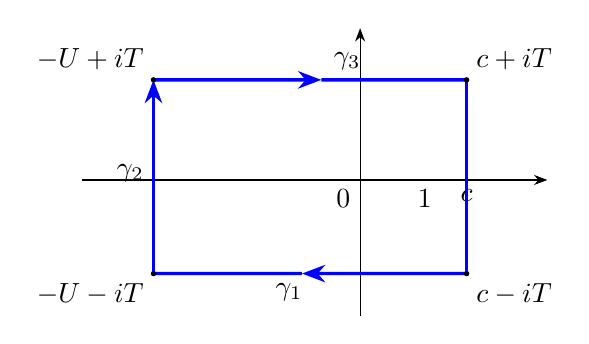
\begin{tikzpicture}[baseline=(current bounding box.center),scale=0.82,>=Stealth]
		\draw[->] (-4.3,0) -- (2.9,0);
		\draw[->] (0,-2.1) -- (0,2.35);
		\node[below left] at (0,0) {$0$};
		\node[below] at (1,0) {$1$};
		\node[below] at (1.65,0) {$c$};
		\coordinate (A) at (1.65,-1.45);
		\coordinate (B) at (-3.2,-1.45);
		\coordinate (C) at (-3.2,1.55);
		\coordinate (D) at (1.65,1.55);
		\draw[blue,very thick,->] (A) -- (-0.9,-1.45);
		\draw[blue,very thick] (-0.9,-1.45) -- (B);
		\node[below] at (-1.1,-1.45) {$\gamma_1$};
		\draw[blue,very thick,->] (B) -- (C);
		\node[left] at (-3.2,0.1) {$\gamma_2$};
		\draw[blue,very thick,->] (C) -- (-0.6,1.55);
		\draw[blue,very thick] (-0.6,1.55) -- (D);
		\node[above] at (-0.2,1.55) {$\gamma_3$};
		\draw[blue,very thick] (D) -- (A);
		\fill (A) circle (1.2pt) node[below right] {$c-iT$};
		\fill (D) circle (1.2pt) node[above right] {$c+iT$};
		\fill (B) circle (1.2pt) node[below left] {$-U-iT$};
		\fill (C) circle (1.2pt) node[above left] {$-U+iT$};
	\end{tikzpicture}
	\]

	先估计 $I_2$。由于在 $\Re(s)<-1$ 且 $|s+2n|\geq 1/4$ 时有
	\[
		\frac{\zeta'}{\zeta}(s)\ll \log|s|,
	\]
	所以
	\[
		I_2
		\ll
		\int_{-T}^{T}
		\log(U+|t|)\frac{x^{-U}}{U}\,dt
		\ll
		\frac{T\log T\log U}{Ux^U}
		\longrightarrow 0
		\qquad (U\to\infty).
	\]

	接着估计 $I_1+I_3$。由于区间 $[T-1,T+1]$ 中至多有 $O(\log T)$ 个非平凡零点 $\rho$，
	所以总可以选择
	\[
		\widetilde T\in[T-1,T+1]
	\]
	使得
	\[
		|\Im\rho-\widetilde T|\gg (\log T)^{-1}
	\]
	对所有非平凡零点 $\rho$ 成立。于是可以假设 (10.4) 中的参数 $T$ 满足
	\begin{equation}
		|\Im\rho-T|\gg \frac1{\log T}
		\qquad
		\text{对所有非平凡零点 }\rho\text{ 成立}.
		\tag{10.8}
	\end{equation}
	因为把 $T$ 换成 $\widetilde T$ 引入的误差至多为
	\[
		\sum_{\substack{\rho\\ T-1\leq|\Im\rho|\leq T+1}}
		\frac{x^\rho}{\rho}
		\ll
		x
		\sum_{\substack{\rho\\ T-1\leq|\Im\rho|\leq T+1}}
		\frac1{|\rho|}
		\ll
		\frac{x}{T}\log T,
	\]
	这可以吸收到 (10.4) 的误差项中。

	由 Lemma 10.1，对所有满足 $-1\leq\sigma\leq2$ 且 $|t|\geq2$ 的
	$s=\sigma+it$，有
	\[
		\frac{\zeta'}{\zeta}(s)
		=
		\sum_{\substack{\rho\\ |\Im\rho-t|<1}}
		\frac1{s-\rho}
		+
		O(\log |t|).
	\]
	再由 (10.8)，当 $s=\sigma+iT$ 且 $-1\leq\sigma\leq2$ 时，
	\[
		\left|\frac{\zeta'}{\zeta}(s)\right|
		\ll
		\log T
		+
		\sum_{\substack{\rho\\ |\Im\rho-T|<1}}
		\frac1{|s-\rho|}
		\ll
		(\log T)^2.
	\]
	因此
	\[
		I_1+I_3
		\ll
		\int_{-U}^{-1}
		\left|\frac{\zeta'}{\zeta}(s)\right|
		\left|\frac{x^s}{s}\right|\,d\sigma
		+
		\int_{-1}^{c}
		\left|\frac{\zeta'}{\zeta}(s)\right|
		\left|\frac{x^s}{s}\right|\,d\sigma.
	\]
	这里分别沿水平线 $\Im(s)=\pm T$ 积分。于是
	\[
	\begin{aligned}
		I_1+I_3
		&\ll
		\int_{-U}^{-1}
		\log T\,\frac{x^\sigma}{T}\,d\sigma
		+
		\int_{-1}^{c}
		\frac{(\log T)^2x^\sigma}{T}\,d\sigma \\
		&\ll
		\frac{\log T}{T}\cdot\frac{1}{x\log x}
		+
		\frac{(\log T)^2}{T}\cdot\frac{x}{\log x}.
	\end{aligned}
	\]
	把这些估计代入 (10.7)，得到
	\[
	\begin{aligned}
		&
		\frac1{2\pi i}
		\int_{c-iT}^{c+iT}
		-\frac{\zeta'}{\zeta}(s)\frac{x^s}{s}\,ds \\
		&\qquad=
		x
		-
		\sum_{\substack{\rho\\ |\Im\rho|<T}}\frac{x^\rho}{\rho}
		-
		\frac{\zeta'}{\zeta}(0)
		+
		\sum_{m<U/2}\frac{x^{-2m}}{2m}
		+
		O\left(
			\frac{T\log T\log U}{Ux^U}
			+
			\frac{x(\log T)^2}{T\log x}
		\right).
	\end{aligned}
	\]
	\weekmarker{第 14 周}

	注意，上面的误差项关于 $U$ 是一致的。令 $U\to\infty$，得到
	\[
	\begin{aligned}
		&
		\frac1{2\pi i}
		\int_{c-iT}^{c+iT}
		-\frac{\zeta'}{\zeta}(s)\frac{x^s}{s}\,ds \\
		&\qquad=
		x
		-
		\sum_{\substack{\rho\\ |\Im\rho|<T}}\frac{x^\rho}{\rho}
		-
		\frac{\zeta'}{\zeta}(0)
		+
		\sum_{m=1}^{\infty}\frac{x^{-2m}}{2m}
		+
		O\left(
			\frac{x(\log T)^2}{T\log x}
		\right),
	\end{aligned}
	\]
	这推出 (10.6)。结合 (10.5) 与 (10.6)，Theorem 10.3 得证。
\end{proof}

\section{\texorpdfstring{\(\zeta(s)\) 的无零区域}{zeta(s) 的无零区域}}

从显式公式（explicit formula），也就是 Theorem 10.3，推出 $\psi(x)$ 的渐近公式时，
必须知道 $\zeta(s)$ 的非平凡零点 $\rho$ 的位置。本节目标是在临界带（critical strip）
\[
	0\leq \Re(s)\leq 1
\]
中找出一块 $\zeta(s)\neq 0$ 的区域。

我们需要用到下面的初等恒等式：
\begin{equation*}
	3+4\cos\alpha+\cos 2\alpha
	=
	2(1+\cos\alpha)^2
	\geq 0
	\qquad
	(\alpha\in\mathbb R).
	\qquad\text{(10.9)}
\end{equation*}

\begin{theorem}[原文 Theorem 10.4]
	对所有 $t\in\mathbb R\setminus\{0\}$，有
	\[
		\zeta(1+it)\neq 0.
	\]
\end{theorem}

\begin{proof}
	对 $\sigma=\Re(s)>1$，由 Euler 乘积（Euler product）可得
	\[
		\zeta(s)
		=
		\prod_p (1-p^{-s})^{-1}.
	\]
	因此
	\[
	\begin{aligned}
		\log\zeta(s)
		&=
		\sum_p -\log(1-p^{-s}) \\
		&=
		\sum_p\sum_{\ell=1}^{\infty}\frac{1}{\ell p^{\ell s}} \\
		&=
		\sum_p\sum_{\ell=1}^{\infty}
		\frac{1}{\ell p^{\ell\sigma}}
		\exp(-i\ell t\log p).
	\end{aligned}
	\]
	于是
	\[
	\begin{aligned}
		\log|\zeta(s)|
		&=
		\Re\log\zeta(s) \\
		&=
		\sum_p\sum_{\ell=1}^{\infty}
		\frac{\cos(\ell t\log p)}{\ell p^{\ell\sigma}}.
	\end{aligned}
	\]
	从而
	\[
		|\zeta(s)|
		=
		\exp\left(
			\sum_p\sum_{\ell=1}^{\infty}
			\frac{\cos(\ell t\log p)}{\ell p^{\ell\sigma}}
		\right).
	\]
	由此得到
	\begin{equation*}
	\begin{aligned}
		&
		\zeta(\sigma)^3
		|\zeta(\sigma+it)|^4
		|\zeta(\sigma+2it)| \\
		&\qquad=
		\exp\left(
			\sum_p\sum_{\ell=1}^{\infty}
			\frac{
				3+4\cos(\ell t\log p)+\cos(2\ell t\log p)
			}{\ell p^{\ell\sigma}}
		\right)
		\geq 1.
		\qquad\text{(10.10)}
	\end{aligned}
	\end{equation*}
	这里最后一步用到了 (10.9)。

	反设存在 $t_0\in\mathbb R\setminus\{0\}$，使得
	\[
		\zeta(1+it_0)=0.
	\]
	当 $\sigma\to1^+$ 时，有
	\[
		|\zeta(\sigma+it_0)|^4
		\leq
		A(\sigma-1)^4
	\]
	对某个 $A>0$ 成立。同时
	\[
		\zeta(\sigma)\sim\frac1{\sigma-1}
		\qquad(\sigma\to1^+),
	\]
	并且 $|\zeta(\sigma+2it_0)|\leq B(t_0)$ 有界。因此
	\[
		\lim_{\sigma\to1^+}
		\zeta(\sigma)^3
		|\zeta(\sigma+it_0)|^4
		|\zeta(\sigma+2it_0)|
		=
		0,
	\]
	这与 (10.10) 矛盾。
\end{proof}

现在可以用 (10.9) 推出 $\zeta(s)$ 的无零区域。为此，我们处理
$-\zeta'/\zeta(s)$ 而不是 $\log\zeta(s)$，因为前者更容易解析延拓到
$\Re(s)>0$。

\begin{theorem}[原文 Theorem 10.5]
	存在常数 $c>0$，使得对 $\zeta(s)$ 的所有非平凡零点
	\[
		\rho=\beta+i\gamma
	\]
	都有
	\[
		\beta
		<
		1-\frac{c}{\log(|\gamma|+2)}.
	\]
\end{theorem}

\begin{proof}
	对 $\Re(s)>1$，有
	\[
		-\frac{\zeta'}{\zeta}(s)
		=
		\sum_{n=1}^{\infty}\frac{\Lambda(n)}{n^{\sigma+it}}
		=
		\sum_{n=1}^{\infty}
		\frac{\Lambda(n)}{n^\sigma}
		\bigl(\cos(t\log n)-i\sin(t\log n)\bigr).
	\]
	分别把这个公式应用到 $s=\sigma$、$s=\sigma+it$ 与
	$s=\sigma+2it$，并取实部的线性组合，得到
	\begin{equation*}
	\begin{aligned}
		&
		\Re\left(
			-3\frac{\zeta'}{\zeta}(\sigma)
			-4\frac{\zeta'}{\zeta}(\sigma+it)
			-\frac{\zeta'}{\zeta}(\sigma+2it)
		\right) \\
		&\qquad=
		\sum_{n=1}^{\infty}
		\frac{\Lambda(n)}{n^\sigma}
		\bigl(3+4\cos(t\log n)+\cos(2t\log n)\bigr)
		\geq 0.
		\qquad\text{(10.11)}
	\end{aligned}
	\end{equation*}
	其中 $\sigma>1$。

	令
	\[
		\rho_0=\beta_0+i\gamma_0
	\]
	为 $\zeta(s)$ 的一个非平凡零点。先假设 $|\gamma_0|$ 足够大；有限多个小
	$|\gamma_0|$ 的零点可以通过缩小最终的常数 $c$ 吸收。

	由 Lemma 10.1，当 $1<\sigma\leq2$ 时，
	\[
		-\frac{\zeta'}{\zeta}(s)
		=
		-\sum_\rho
		\left(
			\frac1{s-\rho}
			+\frac1{\rho}
		\right)
		+
		O(\log |t|)
	\]
	在 $s=\sigma+it$ 附近可用，其中 $\rho$ 遍历非平凡零点。注意对每个非平凡零点
	$\rho$，当 $\Re(s)>1$ 时，
	\[
		\Re\left(\frac1{s-\rho}\right)
		=
		\frac{\Re(s-\rho)}{|s-\rho|^2}
		\geq 0,
		\qquad
		\Re\left(\frac1{\rho}\right)
		=
		\frac{\Re\rho}{|\rho|^2}
		\geq 0.
	\]
	于是，对 $s=\sigma+i\gamma_0$，除 $\rho=\beta_0+i\gamma_0$ 外，
	把求和中的其他零点都舍去，得到
	\[
	\begin{aligned}
		\Re\left(
			-\frac{\zeta'}{\zeta}(\sigma+i\gamma_0)
		\right)
		&\leq
		-\Re\frac{1}{\sigma+i\gamma_0-(\beta_0+i\gamma_0)}
		+
		C\log(|\gamma_0|+2) \\
		&=
		-\frac1{\sigma-\beta_0}
		+
		C\log(|\gamma_0|+2),
	\end{aligned}
	\]
	其中 $1<\sigma\leq2$，而 $C>0$ 是足够大的常数。

	类似地，对 $s=\sigma+2i\gamma_0$，把求和中的所有零点都舍去，得到
	\[
		\Re\left(
			-\frac{\zeta'}{\zeta}(\sigma+2i\gamma_0)
		\right)
		\leq
		C\log(|\gamma_0|+2),
		\qquad
		1<\sigma\leq2.
	\]
	最后，由于
	\[
		-\frac{\zeta'}{\zeta}(s)\sim\frac1{s-1}
		\qquad(s\to1),
	\]
	所以
	\[
		-\frac{\zeta'}{\zeta}(\sigma)
		<
		\frac1{\sigma-1}+C,
		\qquad
		1<\sigma\leq2.
	\]
	把这三个估计代入 (10.11)，得到
	\[
		0
		\leq
		\Re\left(
			-3\frac{\zeta'}{\zeta}(\sigma)
			-4\frac{\zeta'}{\zeta}(\sigma+i\gamma_0)
			-\frac{\zeta'}{\zeta}(\sigma+2i\gamma_0)
		\right)
		<
		\frac3{\sigma-1}
		-
		\frac4{\sigma-\beta_0}
		+
		C\log(|\gamma_0|+2),
	\]
	其中 $C$ 可以取得足够大。

	现在取
	\[
		\sigma
		=
		1+\frac{\delta}{\log(|\gamma_0|+2)},
	\]
	其中 $\delta>0$ 是待定常数。经过简单变形，得到
	\[
		\beta_0
		\leq
		1
		-
		\left(
			\frac{4\delta}{3+C\delta}
			-
			\delta
		\right)
		\frac1{\log(|\gamma_0|+2)}
	\]
	例如取 $\delta=(3C)^{-1}$，就得到所需结论。
\end{proof}

\section{素数定理的证明}

在证明显式公式并掌握 $\zeta(s)$ 的一个无零区域之后，我们可以证明
\[
	\psi(x)=\sum_{n\leq x}\Lambda(n)
\]
的渐近公式。

\begin{theorem}[素数定理；原文 Theorem 10.6]
	存在常数 $c>0$，使得
	\[
		\psi(x)
		=
		x+O\left(xe^{-c\sqrt{\log x}}\right).
	\]
\end{theorem}

\begin{proof}
	由 Theorem 10.3，有
	\begin{equation*}
	\begin{aligned}
		\psi_0(x)
		&=
		x
		-
		\sum_{\substack{\rho\\ |\Im\rho|<T}}\frac{x^\rho}{\rho}
		-
		\frac{\zeta'}{\zeta}(0)
		-
		\frac12\log(1-x^{-2}) \\
		&\qquad+
		O\left(
			\frac{x}{T}(\log xT)^2
			+
			\log x\min\left(1,\frac{x}{T\langle x\rangle}\right)
		\right).
		\qquad\text{(10.12)}
	\end{aligned}
	\end{equation*}
	先估计零点和。由 Lemma 9.9，
	\[
		\sum_{\substack{\rho\\ |\Im\rho|<T}}\frac1{|\rho|}
		\ll
		\sum_{n\leq T}
		\frac1n
		\sum_{\substack{\rho\\ n<|\Im\rho|\leq n+1}}1
		\ll
		\sum_{n\leq T}\frac{\log n}{n}
		\ll
		\log^2 T.
	\]
	又由 Theorem 10.5，若 $\rho=\beta+i\gamma$ 且 $|\gamma|<T$，则
	\[
		\beta
		=
		\Re\rho
		<
		1-\frac{c}{\log(|\gamma|+2)}.
	\]
	因此
	\[
		|x^\rho|
		=
		x^\beta
		\ll
		x\exp\left(-c\frac{\log x}{\log T}\right).
	\]
	于是
	\[
		\sum_{\substack{\rho\\ |\Im\rho|<T}}
		\frac{x^\rho}{\rho}
		\ll
		x\exp\left(-c\frac{\log x}{\log T}\right)\log^2T.
	\]
	因为 $\psi(x)-\psi_0(x)\ll\log x$，将这些估计代入 (10.12)，得到
	\[
		\psi(x)
		=
		x
		+
		O\left(
			x\exp\left(-c\frac{\log x}{\log T}\right)\log^2T
			+
			\frac{x}{T}(\log xT)^2
			+
			\log x
		\right).
	\]
	取
	\[
		T=e^{\sqrt{\log x}}
	\]
	使两个主要误差项平衡，就得到
	\[
		\psi(x)
		=
		x+O\left(xe^{-c\sqrt{\log x}}\right),
	\]
	其中 $c>0$ 可能与上文不同。
\end{proof}

由 Abel 求和公式（Abel summation）还可以得到 $\pi(x)$ 的渐近公式。为此定义
\[
	\operatorname{Li}(x)
	:=
	\int_2^x\frac{du}{\log u}.
\]

\begin{theorem}[原文 Theorem 10.7]
	存在常数 $c>0$，使得
	\[
		\pi(x)
		=
		\operatorname{Li}(x)
		+
		O\left(xe^{-c\sqrt{\log x}}\right).
	\]
\end{theorem}

\begin{proof}
	回忆 Chebyshev 函数
	\[
		\theta(x)=\sum_{p\leq x}\log p.
	\]
	由
	\[
		\theta(x)=\psi(x)+O(\sqrt{x}\log x)
	\]
	以及 Theorem 10.6，可知
	\begin{equation*}
		\theta(x)
		=
		x+O\left(xe^{-c\sqrt{\log x}}\right).
		\qquad\text{(10.13)}
	\end{equation*}
	由 Abel 求和，
	\[
	\begin{aligned}
		\pi(x)
		&=
		\sum_{p\leq x}\frac1{\log p}\log p \\
		&=
		\int_{1.5}^{x}\frac1{\log u}\,d\sum_{p\leq u}\log p \\
		&=
		\frac{\theta(x)}{\log x}
		+
		\int_{1.5}^{x}\frac{\theta(u)}{u\log^2u}\,du.
	\end{aligned}
	\]
	将 (10.13) 代入，得到
	\[
		\pi(x)
		=
		\frac{x}{\log x}
		+
		\int_{1.5}^{x}\frac{du}{\log^2u}
		+
		O\left(
			xe^{-c\sqrt{\log x}}
			+
			\int_{1.5}^{x}\frac{u e^{-c\sqrt{\log u}}}{u\log^2u}\,du
		\right).
	\]
	对主项积分分部，有
	\[
	\begin{aligned}
		\frac{x}{\log x}
		+
		\int_{1.5}^{x}\frac{du}{\log^2u}
		&=
		\frac{x}{\log x}
		+
		\left(-\frac{u}{\log u}\right)_{1.5}^{x}
		+
		\int_{1.5}^{x}\frac{du}{\log u} \\
		&=
		\operatorname{Li}(x)+O(1).
	\end{aligned}
	\]
	对误差项，注意函数
	\[
		u\longmapsto u e^{-c\sqrt{\log u}}
	\]
	是递增的，因此
	\[
		\int_{1.5}^{x}
		\frac{u e^{-c\sqrt{\log u}}}{u\log^2u}\,du
		\ll
		xe^{-c\sqrt{\log x}}
		\int_{1.5}^{\infty}\frac{du}{u\log^2u}
		\ll
		xe^{-c\sqrt{\log x}}.
	\]
	综上，
	\[
		\pi(x)
		=
		\operatorname{Li}(x)
		+
		O\left(xe^{-c\sqrt{\log x}}\right).
	\]
\end{proof}

\begin{remark}[原文 Remark]
	对任意 $A\in\mathbb N$，反复使用分部积分，可得
	\[
		\operatorname{Li}(x)
		=
		\frac{x}{\log x}
		\sum_{n=0}^{A-1}\frac{n!}{(\log x)^n}
		+
		O\left(\frac{x}{(\log x)^{A+1}}\right).
	\]
\end{remark}

\begin{theorem}[原文 Theorem 10.8]
	设 $0\leq\theta<1$。若 $\zeta(s)$ 的所有零点 $\rho$ 都满足
	\[
		\Re\rho\leq\theta,
	\]
	则
	\[
		\psi(x)
		=
		x+O\left(x^\theta(\log x)^2\right).
	\]
	反过来，如果
	\[
		\psi(x)=x+O(x^\theta),
	\]
	则 $\zeta(s)$ 的所有零点 $\rho$ 都满足
	\[
		\Re\rho\leq\theta.
	\]
\end{theorem}

\begin{proof}
	先证明正向。若 $\Re\rho\leq\theta$，则
	\[
		|x^\rho|\leq x^\theta,
	\]
	所以
	\[
		\left|
		\sum_{\substack{\rho\\ |\Im\rho|<T}}
		\frac{x^\rho}{\rho}
		\right|
		\ll
		x^\theta\log^2T.
	\]
	由 $\psi_0(x)$ 的显式公式可得
	\[
		\psi(x)
		=
		x
		+
		O\left(
			x^\theta(\log T)^2
			+
			\frac{x}{T}(\log xT)^2
			+
			\log x
		\right).
	\]
	取 $T=x^{1-\theta}$，得到
	\[
		\psi(x)
		=
		x+O\left(x^\theta(\log x)^2\right).
	\]

	现在证明反向。设
	\[
		\psi(x)=x+O(x^\theta),
	\]
	并记
	\[
		R(x)=\psi(x)-x.
	\]
	当 $\Re(s)>1$ 时，由 Abel 求和可得
	\[
	\begin{aligned}
		-\frac{\zeta'}{\zeta}(s)
		&=
		\sum_{n=1}^{\infty}\frac{\Lambda(n)}{n^s} \\
		&=
		\lim_{x\to\infty}
		\int_1^x \frac1{\xi^s}\,d\sum_{n\leq\xi}\Lambda(n) \\
		&=
		s\int_1^\infty \psi(\xi)\xi^{-s-1}\,d\xi \\
		&=
		s\int_1^\infty \xi^{-s}\,d\xi
		+
		s\int_1^\infty R(\xi)\xi^{-s-1}\,d\xi \\
		&=
		\frac{s}{s-1}
		+
		s\int_1^\infty R(\xi)\xi^{-s-1}\,d\xi.
	\end{aligned}
	\]
	由于
	\[
		R(\xi)=O(\xi^\theta),
	\]
	积分
	\[
		\int_1^\infty R(\xi)\xi^{-s-1}\,d\xi
	\]
	在 $\Re(s)>\theta$ 绝对收敛。因此 $-\zeta'/\zeta(s)$ 在
	$\Re(s)>\theta$ 的唯一奇点是 $s=1$。所以 $\zeta(s)$ 没有满足
	$\Re\rho>\theta$ 的零点。
\end{proof}

回忆
\[
	\frac{\zeta'}{\zeta}(s)
	=
	-\frac1{s-1}
	+
	\sum_\rho\left(\frac1{s-\rho}+\frac1{\rho}\right)
	+
	\sum_{m=1}^{\infty}
	\left(\frac1{s+2m}-\frac1{2m}\right)
	+
	\frac{\gamma}{2}
	+
	\frac{\log\pi}{2}
	+
	B.
\]
因此一旦掌握相应工具，还可以得到下面这些进一步结果。

\medskip
\noindent\textbf{Theorem A.}
设 $\chi$ 是模 $q$ 的 Dirichlet character（Dirichlet 特征）。如果
$\chi\neq\chi_0$ 且
\[
	q\leq(\log x)^A,
\]
则存在 $c(A)>0$，使得
\[
	\sum_{n\leq x}\Lambda(n)\chi(n)
	\ll
	xe^{-c(A)\sqrt{\log x}}.
\]

\medskip
\noindent\textbf{Theorem B.}
设 $A>1$ 固定。存在 $C(A)>0$，使得如果 $q\leq(\log x)^A$，则
\[
	\psi(x;q,a)
	:=
	\sum_{\substack{n\leq x\\ n\equiv a\pmod q}}\Lambda(n)
	=
	\frac{x}{\varphi(q)}
	+
	O\left(xe^{-C(A)\sqrt{\log x}}\right).
\]

\medskip
\noindent\textbf{Theorem C.}
在对所有 $L(s,\chi)$ 的广义 Riemann 假设（generalized Riemann hypothesis）下，
\[
	\psi(x;q,a)
	=
	\frac{x}{\varphi(q)}
	+
	O\left(x^{1/2}\log^2 x\right).
\]


\backmatter
% 需要参考文献时，取消下一行注释。
% \printbibliography[heading=bibintoc]

\end{document}
